% Logic_Quantum.tex — Lecture Notes in Logic, with Applications to Quantum Foundations
%
% Compile: latexmk (uses latexmkrc at the repository root) or
%          pdflatex Logic_Quantum; bibtex Logic_Quantum; pdflatex ...; pdflatex ...
% Engine:  pdfLaTeX

\documentclass{scrartcl}

% ═════════════════════════════════════════════════════════════════════════════
% ┃ ALL \usepackage, macro, and environment declarations live in                ┃
% ┃ Logic_Quantum.sty (loaded below), which loads this document's packages,      ┃
% ┃ the vendored shared packages from _packages/, and then this document's       ┃
% ┃ additions. Do NOT add \usepackage / \newcommand / \newtheorem here. This     ┃
% ┃ preamble carries ONLY the document class, that one style package, and        ┃
% ┃ semantic metadata. See STYLE.md.                                             ┃
% ═════════════════════════════════════════════════════════════════════════════
% Where the vendored shared .sty files live (makes plain pdflatex work without TEXINPUTS).
\makeatletter\def\input@path{{../_packages/}{_packages/}}\makeatother
\usepackage{Logic_Quantum}

% ─── Document Metadata ──────────────────────────────────────────────────────
\title{ \normalsize \textsc{}
		\\ [2.0cm]
		\HRule{1.5pt} \\
		\LARGE \textbf{\uppercase{Lecture Notes in Logic,\\ with Applications to Quantum Foundations}
		\HRule{2.0pt} \\ [0.6cm] \LARGE{} \vspace*{10\baselineskip}}
		}
    \subtitle{The University of Texas at San Antonio, Summer-Fall  2025}
\date{Last edit: \today, \currenttime \ UTC }
\author{Lecture notes coordinated by Olivia Aubone\\
{Faculty advisors: Eduardo Dueñez, José Iovino}\\
}

\begin{document}

\maketitle
\newpage

\tableofcontents
\newpage

% ------------------------------------------------------------------------------



\setcounter{section}{-1}
\section{Preface: Propositional logic}

In this section, $\mathscr{S}$ will denote a fixed set of syntactic symbols that we will call \emph{sentence symbols}.

Starting with the set $\mathscr{S}$ of sentence symbols, we build a collection of ``words'' (i.e., finite strings of symbols) called the \emph{sentences of $\mathscr{S}$}; we will call these these simply ``sentences'' since $\mathscr{S}$ remains fixed throughout. The definition of sentence is recursive in the following sense; the symbols in $\mathscr{S}$ are defined as the sentences of lowest complexity, and then, assuming that we have already defined the sentences of up to a given level of complexity, we define the sentences of the next level of complexity. The formal definition is as follows:


\begin{definition}
A \emph{sentence (of $\mathscr{S}$)} is any finite string of symbols produced by any finite number of applications of the following formation rules:
\begin{enumerate}[i)]
\item Every sentence symbol $S\in\mathscr{S}$ is a sentence;
\item If $\alpha$ is a sentence of $\mathscr{S}$, then $\neg \alpha$ is a sentence of $\mathscr{S}$;

\item If $\alpha,\beta$ are sentences, then $(\alpha \lor \beta)$ is a sentence of $\mathscr{S}$.
\end{enumerate}
We denote the set of all sentences of $\mathscr{S}$ as $L_\mathscr{S}$. 
\end{definition}

Every sentence of $\mathscr{S}$ is a ``word'' of finite length in an alphabet consisting of the symbols in $\mathscr{S}$, the parenthesis symbols ``$($'', ``$)$'', and the connective symbols $\neg$, $\lor$. It is important to emphasize that the sentences of $\mathscr{S}$ are merely syntactic strings. We are not assigning any meaning to them.

By convention, for given sentences $\alpha,\beta$, we regard $(\alpha\land\beta)$ and $(\alpha\to\beta)$ as abbreviations of $\neg(\neg\alpha\lor\neg\beta)$ and $\neg\alpha\lor\beta$, respectively, and we regard $(\alpha\leftrightarrow\beta)$ as an abbreviation of $(\alpha\to\beta)\land (\beta\to\alpha)$.



\begin{definition}

If $S_0,\dots,S_n$ are sentence symbols, an \emph{assignment} for $S_0,\dots,S_n$ is a sequence $v_0,\dots,v_n$ such that $v_i$ is either $0$ or $1$ for each $i\in \{0,\dots,n\}$.

Let $\alpha$ be a sentence in $L_\mathscr{S}$ such that all of the sentence symbols that occur in $\alpha$ are among $S_0,\dots,S_n$.  Given an assignment $v_0,\dots,v_n$ for $S_0,\dots,S_n$, the \emph{value} of $\alpha$, denoted $v(\alpha)$, is defined recursively as follows:

\begin{enumerate}[i)]
\item If $\alpha$ is a sentence symbol $S_i$ where $i\in\{0,\dots,n\}$, then $v(\alpha) = v_i$;
\item If $\alpha$ is $\neg \beta$,  then $v(\alpha) = 1 - v(\beta)$;
\item If $\alpha$ is $(\beta \wedge \gamma)$, then $v(\alpha) = \min(v(\beta), v(\gamma))$.
\end{enumerate}
\end{definition}

\begin{definition}
\label{D:propositional tautology}
Let $\alpha$ be a sentence in $L_\mathscr{S}$ such that all of the sentence symbols that occur in $\alpha$ are among $S_0,\dots,S_n$. We call $\alpha$ a \emph{propositional tautology} if $v(\alpha) = 1$ for every assignment $v_0,\dots, v_n$.
\end{definition}


\section{First-Order Logic}
\label{S:Logic}


\subsection{Structures}




\begin{definition}
\label{D:structure}
A \emph{(one-sorted) structure}, denoted 
\[
\mathfrak{M} = (M,(c_i)_{i\in I}, (f_j)_{j\in J}, (P_k)_{k\in K}) \text{,}
\]
is a single set $M$, also called the \emph{universe} or \emph{domain} of  $\mathfrak{M}$, together with:
\begin{enumerate}[i)]
\item Certain specifically named (\say{distinguished}) elements of $M$ called the \emph{constants} of $\FM$,
\item Operations $f\colon M^n\to M$, each of some arity $n\in\mathbb{N}$, and
\item Relations, also called predicates, $P\colon M^n\to \{\top,\bot\}$, each of some arity $n\in\mathbb{N}$.

(The set $\{\top,\bot\}$ may be thought of as a set containing the logical values ``true" and ``false".)

\end{enumerate}

We will assume tacitly that all structures come with the binary predicate $\{(x,x):x\in M\}$ of equality, denoted $=$.


The \emph{elements} of a structure are the elements of the universe of the structure.

\end{definition}

Note that a structure need not have operations, predicates, and constants. For instance, a group $\mathscr{G}=( G, *, e)$ (where $*$ is the group operation and $e$ is the identity of $\mathscr{G}$) does not come with any predicates; similarly, classical algebraic structures such as rings and fields have only operations. On the other hand, a partial order $(\Sigma,\le)$ and a graph $G=(E,R)$ (where $E$ is the set of edges of $G$ and $R$ is the incidence relation) are examples of relational structures, i.e., structures that do not include any operations. An ordered group $G=( G, *, e, \le)$ has a binary operation~$*$, a constant $e$, and a binary predicate $\le$.


Note that the constants of a structure can be regarded as $0$-ary functions. For this reason, we often omit a separate list of the constants of a structure; that is, we assume that the constants are already included in the list of functions of the structure.

According to the preceding definition, each structure has only one domain. However, in standard mathematical practice, we encounter structures that have multiple domains. Such domains are called the \emph{sorts} of the structure. As an example, a vector space requires two sorts: a sort for vectors and a sort for scalars. The scalar multiplication operation takes in a scalar and a vector as input and produces a vector as output. This simple example illustrates the fact that, for multisorted structures, each of the operations and predicates of a given structure must equipped not only with an arity, but also a specified sort for each of its variables. In Definition~\ref{D:structure}, for generality, we could have included a definition of structure that includes multisorted structures. However, since the specification of a sort for each variable of each function or relation of a structure, as well as each constant of the structure,  often makes the notation cumbersome, we restrict our attention almost exclusively to one-sorted structures, i.e., structures with a single sort (called the \emph{domain} or \emph{universe} of the structure). It should be clear how our results extend to multisorted contexts.



\begin{notation}
In contexts where we speak of a structure $\mathfrak{M}$ and we need to emphasize that the universe of $\mathfrak{M}$ is $M$ in a context where it is not necessary to specify the operations, or predicates or $\mathfrak{M}$, we may write $\mathfrak{M}=(M,\dots)$.
\end{notation}

\subsection{Syntax: Vocabularies, terms, formulas, and sentences}



In this section, we introduce the basic definitions of \emph{language} and \emph{theory} that are standard in logic and that will be used throughout the notes. Readers familiar with these notions may skip this section and jump directly to Section~\ref{S:topology}.


\begin{definition}
A \emph{vocabulary} 
\[
V = \big(\,(\mathbb{c}_i)_{i\in I}, (\mathbb{f}_j)_{j\in J}, (\mathbb{P}_k)_{k\in K}\,\big)
\]
is a collection of:
\begin{enumerate}[i)]
\item \emph{Constant symbols} $(\mathbb{c}_i)_{i\in I}$,
\item \emph{Operation symbols} $(\mathbb{f}_j)_{j\in J}$, each with some arity $n_j\in\mathbb{N}$, and
\item \emph{Predicate symbols} $(\mathbb{P}_k)_{k\in K}$, each with some arity $n_k\in\mathbb{N}$.
\end{enumerate}
\end{definition}

Fix a vocabulary $V=((\mathbb{c}_i)_{i\in I}, (\mathbb{f}_j)_{j\in J}, (\mathbb{P}_k)_{k\in K})$ and a countable collection of formal symbols $x,y,z\dots$ called \emph{variable symbols}, or simply ``variables".

A \emph{term} of $V$ is a finite string of symbols built from the constant and function symbols in $V$, the variable symbols, the parenthesis symbols ``$($'', ``$)$'', and the comma symbol ``$,$'' as follows:

\begin{definition}
A \emph{term} of $V$ is any finite string of symbols produced by any finite number of applications of the following formation rules:
\begin{enumerate}[i)]
\item Each constant symbol is a term.
\item Each variable is a term.
\item If $\mathbb{f}$ is an $n$-ary operation and $\tau_1, \dots, \tau_n$ are terms, then $\mathbb{f}(\tau_1, \dots, \tau_n)$ is a term.
\end{enumerate}

A \emph{closed term} is a term in which no variables appear.
\end{definition}


A \emph{formula} of $V$ is a finite string of symbols built from the terms of $V$, the predicate symbols of $V$, the equality symbol $=$, the connective symbols $\land$ ,$\lor$, $\to$, $\neg$, the quantifier symbols $\exists,\forall$, and the parenthesis symbols $)$ and $($ as follows.

\begin{definition}
An \emph{atomic $V$-formula} is any syntactic expression either of the form 
\[
\mathbb{P}(\tau_1,\dots ,\tau_n),
\]
where $\mathbb{P}$ is a predicate symbol and $\tau_1,\dots ,\tau_n$ are terms, or of the form 
\[
\tau_1=\tau_2,
\]
where $=$ is a symbol for equality and $\tau_1,\tau_2$ are terms.

Other $V$-formulas are defined recursively as follows. If $\varphi, \psi $ are $V$-formulas, then:

\begin{enumerate}[i)]
\item $(\varphi\wedge\psi)$, $(\varphi\vee\psi)$, and $(\varphi\to\psi)$ are $V$-formulas,

\item $\neg\varphi$ is a $V$-formula,

\item For any variable $x$, $(\exists x)\varphi$ and $(\forall x)\varphi$ are $V$-formulas.
\end{enumerate}


\end{definition}


When a formal variable symbol $x$ is under the scope of a quantifier in a formula $\phi$ (by application of the last rule of formation), we say that $x$ occurs \emph{bound} in $\phi$.



\begin{definition}
A $V$-\emph{sentence} $\varphi$ is a $V$-formula in which no variables are free; that is, every occurrence of a variable symbol in $\varphi$ must be bound by a quantifier in $\phi$. A $V$-\emph{theory} is a set of sentences.
\end{definition}

\begin{definition}
The \emph{first-order language} $L_V$ is the set which consists of all $V$-formulas.
\end{definition}

\begin{definition}
A first-order $V$-formula $\phi$ is called a \emph{prime formula} if
\begin{enumerate}[i)]
\item $\phi$ is an atomic formula, or
\item $\phi$ is $(\exists v)\psi$ for some $\psi\in L_V$, or
\item $\phi$ is $(\forall v)\psi$ for some $\psi\in L_V$.
\end{enumerate}

\end{definition}

\begin{definition}
\label{D:Tautology}
A first-order formula $V$-formula $\phi$ is called a \emph{tautology} if it can be obtained from a propositional tautology $\psi\in L_\mathscr{S}$ (see Definition~\ref{D:propositional tautology}), where $\mathscr{S}$ is a set of sentence symbols, by simultaneously and uniformly substituting the sentence symbols in $\mathscr{S}$ for the prime formulas of $L_V$.
\end{definition}

We emphasize terms and formulas are merely symbolic expressions. We are not assigning any meaning to them. This will be done in the next section through the concepts of \emph{interpretation}, \emph{satisfaction}, \emph{model}, and \emph{type}.


\subsection{Semantics: Interpretations, models, types, and elementary extensions}
\label{S:Semantics}


\begin{definition}
Given a vocabulary
\[
V = \big(\,(\mathbb{c}_i)_{i\in I}, (\mathbb{f}_j)_{j\in J}, (\mathbb{P}_k)_{k\in K}\,\big),
\]
a $V$-\emph{structure} is any structure of the form 
\[
\mathfrak{M} =  \left( M, (c_i)_{i\in I}, (f_j)_{j\in J}, (P_k)_{k\in K}\right) = 
\left( M, (\mathbb{c}_i^{\mathfrak{M}})_{i\in I}, (\mathbb{f}_j^{\mathfrak{M}})_{j\in J}, (\mathbb{P}_k^{\mathfrak{M}})_{k\in K}\right)
\text{.}
\]
For every $i\in I,j\in J,k\in K$, the objects
\[
\mathbb{c}_i^{\mathfrak{M}}, \quad \mathbb{f}_j^{\mathfrak{M}}, \quad\mathbb{P}_k^{\mathfrak{M}}
\]
are called the \emph{interpretations}, in $\FM$, of  the symbols $\mathbb{c}_i$,  $\mathbb{f}_j$ and $\mathbb{P}_k$, respectively.


If $\FM$ is as above, a \emph{substructure} of $\FM$ is any $V$-structure of the form
\[
\mathfrak{N} =  \left( N, (c_i)_{i\in I}, (f_j)_{j\in J}, (P_k)_{k\in K}\right) = \left( N, (\mathbb{c}^{\mathfrak{N}}_i)_{i\in I},(\mathbb{f}^{\mathfrak{N}}_j)_{j\in J}, (\mathbb{P}^{\mathfrak{N}}_k)_{k\in K} \right),
\]
where $N$ is a subset of $M$ that contains all the constants of $\mathfrak{M}$, is closed under all the operations of $\mathfrak{M}$, and such that for every $j\in J$ and every $k\in K$, we have
$\mathbb{f}_j^{\mathfrak{N}}$ and  $\mathbb{P}_k^{\mathfrak{N}}$ as the restrictions of $\mathbb{f}_j^{\mathfrak{M}}$ and  $\mathbb{P}_k^{\mathfrak{M}}$, respectively, to $N$. If $\FN$ is a substructure of $\FM$, we write
$\FN\subseteq \FM$.

\end{definition}

If $\tau$ is a term of $V$ all of whose variables are contained in the set $\{x_1,\dots, x_n\}$, then we may write $\tau$ as $\tau(x_1,\dots,x_n)$, and we refer to $\tau$ as an $n$-ary term.  For such terms, we have a natural interpretation $\tau^{\mathfrak{M}}:M^n\to M$. 

\begin{notation}
If $\varphi$ is a formula and $x_1,\dots,x_n$ is a list of variables, we write 
\[
\varphi(x_1,\dots,x_n)
\]
to indicate that all the free variables of $\phi$ are contained in the set $\{x_1,\dots, x_n\}$.
\end{notation}

If $\varphi(x_1,\dots,x_n)$ is a $V$-formula and $\mathfrak{M}$ is a $V$-structure, then $\varphi(x_1,\dots,x_n)$ is given an interpretation $\varphi^{\mathfrak{M}}:M^n\to \{\top,\bot\}$ by the following recursive rules:
\begin{enumerate}[i)]

\item For atomic $\varphi\equiv \mathbb{P}(\tau_1,\dots, \tau_m)$ on free variables $x_1,\dots,x_n$, let
\begin{align*}
\varphi^{\mathfrak{M}}\colon M^n&\to \{\top,\bot\}\\
\overline{a}=(a_1,\dots,a_n) &\mapsto \mathbb{P}^{\mathfrak{M}}(\tau_1^{\mathfrak{M}},\dots, \tau_m^{\mathfrak{M}})(a_1,\dots,a_n)
\end{align*}

\item For $((\varphi\wedge\psi))^\mathfrak{M}$ on free variables $x_1,\dots,x_n$, let
\[
((\varphi\wedge\psi))^{\mathfrak{M}} \colon M^n \to \{\top,\bot\}
\]
map $\overline{a}$ to $\top$ if and only if $\varphi^\mathfrak{M}(\overline{a}) = \top$ and $\psi^\mathfrak{M}(\overline{a}) = \top$.

For $(\varphi)^\mathfrak{M}$ on free variables $x_1,\dots,x_n$, let
\[
(\neg\varphi)^{\mathfrak{M}} \colon M^n \to \{\top,\bot\}
\]
map $\overline{a}$ to $\top$ if and only if $\varphi^{\mathfrak{M}}(\overline{a}) = \bot$.

The connectives $\vee,\to$ are dealt with analogously.

\item If $x$ is not free in $\varphi$, then $(\forall x(\varphi))^{\mathfrak{M}}$ and $(\exists x(\varphi))^{\mathfrak{M}}$ are both $\varphi^{\mathfrak{M}}$.

\item If $x$ is free in $\varphi\equiv \varphi(x_1,\dots,x_{n+1})$, then let %edit: would it make more sense to write \varphi(x,x_1,\dots,x_n) ?
\[
(\forall x(\varphi))^{\mathfrak{M}}\colon M^n\to \{\top,\bot\}
\]
map $\overline{a}$ to $\top$ if $\varphi^{\mathfrak{M}}(b,\overline{a})=\top$ for all $b\in M$, and $\bot$ otherwise. Also, let 
\[
(\exists x(\varphi))^{\mathfrak{M}}\colon M^n\to \{\top,\bot\}
\]
map $\overline{a}$ to $\top$ if $\varphi^{\mathfrak{M}}(b,\overline{a})=\top$ for some $b\in M$, and $\bot$ otherwise.
\end{enumerate}

In the rest of these notes, we shall identify $\top$ and $\bot$ with 1 and 0, respectively.

\begin{notation}
If $\varphi$ is a sentence, we say $\mathfrak{M}$ \emph{satisfies} $\phi$, denoted
\[
\mathfrak{M}\models \varphi,
\]
if and only if $\varphi^{\mathfrak{M}}=\top$.

More generally, if $\phi(x_1,\dots, x_n)$ is a formula and $(a_1,\dots, a_n)\in M^n$, we write
\[
\mathfrak{M}\models \varphi[a_1,\dots,a_n]
\]
if and only if $\varphi^{\mathfrak{M}}(a_1,\dots,a_n)=\top$.
\end{notation}

Below are the fundamental definitions of model theory.

\begin{definition}
Let $\mathfrak{M}$ be a $V$-structure with universe $M$.

If $\bar a= (a_1,\dots, a_n)\in M^n$, the \emph{(complete) type} of $\bar a$ in $\mathfrak{M}$ is the set %edit: should \bar{a} be defined as an n-tuple in M^n similar to previous notation? I suppose it is any tuple of elements from M
\[
\tp_{\mathfrak M}(\bar a)=
\{\varphi(\bar x)\in L_V \colon \mathfrak{M}\models\varphi[\bar a] \}.
\]

The \emph{complete theory} of $\mathfrak{M}$ is the set
\[ 
\Th(\mathfrak{M}) = \{ \varphi\in L_V \colon \varphi \text{ is a sentence and } \mathfrak{M}\models\varphi \}.
\]
\end{definition}


 

\begin{definition}
If $V$ is a first-order vocabulary, two $V$-structures $\mathfrak{M}$ and $\mathfrak{N}$ are said to be \emph{elementarily equivalent}, written
\[
\mathfrak{M}\equiv\mathfrak{N},
\]
if $\mathfrak{M}$ and $\mathfrak{N}$ satisfy the same sentences, i.e., if
for every sentence $V$-sentence $\varphi$,
\[
\mathfrak{M}\models \varphi
\quad\text{if and only if}\quad
\mathfrak{N} \models \varphi.
\]
If $\mathfrak{M}$ is a substructure of $\mathfrak{N}$, then we say that $\mathfrak{M}$ is an \emph{elementary substructure} of $\mathfrak{N}$, or that $\FM$ is an \emph{elementary extension} of $\FM$, and we write
\[
\mathfrak{M}\prec\mathfrak{N},
\]
if $\FM$ and $\FN$ satisfy the same sentences in an expansion of $V$ that includes a constant symbol for each element of the universe of $\mathfrak{M}$, that is, if whenever $\varphi(x_1,\dots, x_n)$ is a $V$-formula and $a_1,\dots, a_n$ are elements of the universe of $\mathfrak{M}$, 
\[
\mathfrak{M}\models \varphi[a_1,\dots, a_n]
\quad\text{if and only if}\quad
\mathfrak{N} \models \varphi[a_1,\dots, a_n].
\]
\end{definition}

Note that $\mathfrak{M}\equiv\mathfrak{N}$ if and only if $\mathfrak{M}$ and $\mathfrak{N}$ have the same complete theory. Note also that $\mathfrak{M}\prec\mathfrak{N}$ if all tuples of elements of $\FM$ have the same type in both $\FM$ and $\FN$.


\begin{definition}
If $T$ is a theory, we say that $\mathfrak{M}$ is a \emph{model} of $T$, written 
\[
\mathfrak{M}\models T,
\]
if $\mathfrak{M}$ satisfies every sentence in $T$.
A theory is \emph{satisfiable} if it has a model.
\end{definition}


The compactness theorem is one of the cornerstone theorems of first-order logic. It will be proved in~\ref{T:compactness}, \ref{C:compactness from completeness 1}, and~\ref{C:compactness from completeness 2}. using different approaches.

\begin{theorem}[Compactness of first-order logic]
\label{T:compactness from Los}
Let $T$ be a theory. If every finite subset of $T$ is satisfiable, then $T$ is satisfiable.
\end{theorem}


\section{Topology}
\label{S:topology}

\subsection{Topological spaces}

\begin{definition}
\label{D:topological space}
    A \emph{topological space} is a structure $(X, \mathscr{N}_x)_{x\in X}$  that consists of a set $X$ and, for each point $x\in X$, a collection $\mathscr{N}_x$ of subsets of $X$ that satisfy the following properties:

    \begin{enumerate}[i)]
        \item $x\in U$ for every $U\in \mathscr{N}_x$;
        \item If $U,V\in \mathscr{N}_x$, then there exists $W\in \mathscr{N}_x$ such that $W\subseteq U\cap V$;
        \item For every $U\in \mathscr{N}_x$ and every $y\in U$, there exists $V_y\in \mathscr{N}_y$ such that $V_y\subseteq U$.
        
    \end{enumerate}
\end{definition}


Next we introduce an immediate result from the previous definition. The reader should note that Property iii) and the next proposition are equivalent.

\begin{proposition}
\label{P:basic nhoods are open}
    Let $(X, \mathscr{N}_x)_{x\in X}$ be a topological space. For every $U\in \mathscr{N}_x$ and every $y\in U$, there exists $V_y\in \mathscr{N}_y$ such that \[U=\bigcup\limits_{y\in U}V_y\text{.}\]
\end{proposition}

\begin{proof}
  Fix a point $x\in X$, and let $U\in \mathscr{N}_x$ be given.
  By Property iii) above, we have that for every $y\in U$, there is some $V_y\in \mathscr{N}_y$ such that $V_y\subseteq U$.
  Thus, the union of all such $V_y$ is contained in $U$.
  Also, by Property i), we see that for every $y\in U$, we have $y\in V_y\subseteq \bigcup\limits_{y\in U}V_y$. Thus, $U=\bigcup\limits_{y\in U}V_y$.
\end{proof}

\begin{definition}
  Let $( X, \mathscr{N}_x)_{x\in X}$ be a topological space.

  For each $x\in X$, we refer to $\mathscr{N}_x$ as the \emph{neighborhood base} for $x$. 
  The indexed family $(\mathscr{N}_x)_{x\in X}$ is called a \emph{local neighborhood base} on $X$.
  For all $x\in X$, each set $U\in \mathscr{N}_x$ is called a \emph{basic neighborhood} of $x$. A \emph{neighborhood} of $x$ is any superset of a basic neighborhood of $x$.
    
\end{definition}

\begin{definition}
  A set $O\subseteq X$ is called \emph{open} if for every $x\in O$, there exists $V_x\in \mathscr{N}_x$ such that 
  \[
  O=\bigcup\limits_{x\in O}V_x\text{.}
  \]
  
  A set $C\subseteq X$ is called \emph{closed} if $X\setminus C$ is open. Note that $C$ is closed if for every $x\in X$, if every basic neighborhood of $x$ intersects $C$, then $x\in C$.
\end{definition}

Note that, by Proposition~\ref{P:basic nhoods are open}, a subset of $X$ is open if and only it is a union of basic neighborhoods.

\begin{proposition}
\label{P:properties of open sets}

    In any topological space $(X, \mathscr{N}_x)_{x\in X}$, the following properties hold:

    \begin{enumerate}[i)]
        \item Both $\emptyset$ and $X$ are open subsets of $X$ (and evidently also closed);
        \item Any union of open subsets of $X$ is open;
        \item Any finite intersection of open subsets of $X$ is open.
        
    \end{enumerate}
\end{proposition}

\begin{proof}

\leavevmode

\begin{enumerate}[i)]
\item The empty set is open since any condition that must be satisfied by the points in $\emptyset$ is true vacuously. The set $X$ itself is open since, for each point $x\in X$, we may choose $V_x\in \mathscr{N}_x$ arbitrarily so that $X=\bigcup\limits_{x\in X}V_x$.

\item Given any open subsets $(O_i)_{i\in I}$ of $X$, we have that each $O_i$ is a union of basic neighborhoods. Thus, the union $\bigcup\limits_{i\in I}O_i$ is a larger union of basic neighborhoods, and hence also an open subset of $X$.

\item If $O_1$ and $O_2$ are open subsets of $X$, then for each $x\in O_1\cap O_2$, there are $U,V\in \mathscr{N}_x$ such that $U\subseteq O_1$ and $V\subseteq O_2$. By Property ii) of Definition~\ref{D:topological space}, there's $W_x\in \mathscr{N}_x$ such that \[W_x\subseteq U\cap V\subseteq O_1\cap O_2\text{.}\] Thus, $O_1\cap O_2$ is the union of all such $W_x\in \mathscr{N}_x$ that satisfy $W_x\subseteq O_1\cap O_2$ as $x$ ranges over $O_1\cap O_2$.
\end{enumerate}
\end{proof}

Note that an infinite intersection of open sets is not necessarily open, as will be shown in Example \ref{E:basic topological spaces}(a).

\begin{definition}
Let $(X, \mathscr{N}_x)_{x\in X}$ be a topological space.

The \emph{topology} $\mathscr{T}$ on $X$ generated by the local neighborhood base $(\mathscr{N}_x)_{x\in X}$  is the collection of all open subsets of $X$; that is, 
\[
\mathscr{T}= 
\{ O\subseteq X \colon O \text{ is open}\}\text{.}
\]
\end{definition}

Note that two different local neighborhood bases on $X$ can generate the same topology. For instance, examples (a) and (b) below generate the same topology on $\mathbb R$.

\begin{example} Basic examples
\label{E:basic topological spaces}

\begin{enumerate}[(a)]

\item Let $X=\mathbb{R}$, and for each $x\in \mathbb{R}$,  let $\mathscr{N}_x=\{(x-\varepsilon , x+\varepsilon):\varepsilon >0\}$.

We will show that there is an infinite intersection of open subsets of $X$ that is not open. Take, for instance, the infinite intersection \[\bigcap\limits_{n\in \mathbb{N}}(0,1+\frac{1}{n})=(0,1]\text{.}\]
This interval is not open since there is no basic neighborhood $(1-\varepsilon,1+\varepsilon)$ of $1\in X$ that is contained in $(0,1]$.

\item Let $X=\mathbb{R}$, and for each $x\in \mathbb{R}$,  let $\mathscr{N}_x=\{(\alpha , \beta) \colon \alpha<x<\beta, \alpha,\beta\in\mathbb{R} \}$.

\item Let $X=\mathbb{R}^2$, and for each $x\in \mathbb{R}^2$, let $\mathscr{N}_x$ consist of the set of all open disks about $x$ of radius $\varepsilon$ for all $\varepsilon >0$.

\item Let $X$ be any set, and for each $x\in X$, let $\mathscr{N}_x = \{\{x\}\}$; i.e., the only basic neighborhood of $x$ is the singleton $\{x\}$. The resulting topology is called the \emph{discrete} topology on $X$.

Note that, in this topological space, every subset of $X$ is open (since every set is a union of singletons). Hence, every subset is closed as well.

\item Let $X$ be any set, and for each $x\in X$, let $\mathscr{N}_x = \{X\}$. The resulting topology is called the \emph{trivial} (or \emph{indiscrete}) topology on $X$. Note that, in this topological space, only two subsets are open; namely, $\emptyset$ and $X$.

\end{enumerate}

\end{example}


\begin{example} Topological spaces of particular importance to logic
\label{E: logic topological spaces}

\begin{enumerate}[(a)]

\item Fix a first-order vocabulary $V$, and let $X$ be the class that consists of all $V$-structures. For each $V$-sentence $\varphi$, define 
\[
\Mod(\varphi):=\{\mathfrak{N}\in X \colon \mathfrak{N}\models \varphi\}\text{.}
\]
Then, for each $\mathfrak{M}\in X$, let $\mathscr{N}_\mathfrak{M} = \{ \Mod (\varphi): \mathfrak{M}\models \varphi \}$.

We will show that $(X,\mathscr{N}_\mathfrak{M})_{\mathfrak{M}\in X}$ satisfies the three properties of a topological space given in Definition~\ref{D:topological space}.

\begin{proof} Fix a structure $\mathfrak{M}\in X$.

\begin{enumerate}[i)]

\item Let a basic neighborhood $\Mod(\varphi) \in \mathscr{N}_\mathfrak{M}$ be given. By definition, we have $\mathfrak{M}\models \varphi$ and thus $\mathfrak{M}\in\Mod(\varphi)$.

\item Let basic neighborhoods $\Mod(\varphi), \Mod(\psi) \in \mathscr{N}_\mathfrak{M}$ be given.
We need to find a basic neighborhood $W\in \mathscr{N}_\mathfrak{M}$ such that \[W \subseteq \Mod(\varphi)\cap \Mod(\psi)\text{.}\]
It suffices to take $W = \Mod(\varphi\wedge \psi)$ since \[\Mod(\varphi\wedge \psi) = \Mod(\varphi)\cap \Mod(\psi)\text{.}\]

\item Let a basic neighborhood $\Mod(\varphi) \in \mathscr{N}_\mathfrak{M}$ and a structure $\mathfrak{N}\in \Mod(\varphi)$ be given.
We need to find a basic neighborhood $W_\mathfrak{N}\in \mathscr{N}_\mathfrak{N}$ such that \[W_\mathfrak{N} \subseteq \Mod(\varphi)\text{.}\]
It suffices to take $W_\mathfrak{N} = \Mod(\varphi)$ since, by definition, $\mathfrak{N}\models \varphi$ and thus $\Mod(\varphi)\in\mathscr{N}_\mathfrak{N}$ where, clearly, $\Mod(\varphi)\subseteq \Mod(\varphi)$.
\end{enumerate}
\end{proof}

\item Fix a structure $\mathfrak{M}=(M, \mathscr{P})$ where $\mathscr{P}$ is a set of prediactes, and assume each $P\in \mathscr{P}$ is unary of the form $P\colon M\to [0,1]$. For each $a\in M$, let 
\[
\operatorname{tp}(a) = (P(a))_{P\in \mathscr{P}}\in [0,1]^\mathscr{P}\
\]
be the \emph{quantifier-free type} of $a$.

Then we have a map $\operatorname{tp} \colon M\to [0,1]^\mathscr{P}$ which maps each element $a$ in $M$ to the type of $a$.

Fix finitely many $P_1,\dots,P_n\in\mathscr{P}$, and fix $\varepsilon > 0$. Given $a\in M$, define 
\[
V_a(P_1,\dots, P_n,\varepsilon):= \left\{b\in M \colon |P_i(b)-P_i(a)|<\varepsilon \text{ for all } i\in \{ 1,\dots, n\} \right\} \text{.}
\]
We define a neighborhood base around $a\in M$ by 
\[
\mathscr{N}_a = \left\{ V_a(P_1,\dots, P_n,\varepsilon) \colon \varepsilon >0, P_1,\dots,P_n\in\mathscr{P}, n\in\mathbb{N} \right\}\text{.}
\]

We will show that $(M,\mathscr{N}_a)_{a\in M}$ satisfies the three properties of a topological space given in Definition~\ref{D:topological space}.

\begin{proof} Fix an element $a\in M$.

\begin{enumerate}[i)]

\item Let a basic neighborhood $V_a(\varepsilon, P_1,\dots, P_n)\in\mathscr{N}_a$ be given. Since \[|P_i(a)-P_i(a)| = 0 <\varepsilon\] for all $P_i\in \mathscr{P}$ and all $\varepsilon > 0$, it immediately follows that $a\in V_a(P_1,\dots, P_n,\varepsilon)$.

\item Let basic neighborhoods $V_a(P_1,\dots, P_m,\varepsilon), U_a(\delta, Q_1,\dots, Q_n) \in\mathscr{N}_a$ be given. We need to find a basic neighborhood $W\in \mathscr{N}_a$ such that \[
W \subseteq V_a(P_1,\dots, P_m, \varepsilon) \cap U_a(\delta, Q_1,\dots, Q_n) \text{.}
\]
It suffices to take 
\[
W = W_a(P_1,\dots, P_m, Q_1,\dots, Q_n,\min(\varepsilon,\delta))
\]
since for all $b\in W$, we have \[
|P(b)-P(a)|<\min(\varepsilon,\delta) \text{ for all } P\in\{P_1,\dots, P_m, Q_1,\dots, Q_n\}\text{,}
\]
and hence $b\in V_a\cap U_a$.

\item Let a basic neighborhood $V= V_a(P_1,\dots, P_n,\varepsilon)\in\mathscr{N}_a$ and an element $b\in V$ be given. We need to find a basic neighborhood $W\in \mathscr{N}_b$ such that $W \subseteq V$.
Letting 
\[
\delta = \sup\left\{|P_i(b)-P_i(a)|\colon i\in\{1,\dots,n\}\right\}\text{,}
\]
we see that it suffices to take $W = W_b(P_1,\dots, P_n,\varepsilon -\delta)\in\mathscr{N}_b$ since, for any $c\in W$, we have
\begin{align*}
|P_i(c)-P_i(a)| &= |P_i(c)-P_i(b)-P_i(a)+P_i(b)| \\
&\leq |P_i(c)-P_i(b)| + |P_i(b)-P_i(a)| \tag{By the Triangle Inequality} \\
&\leq |P_i(c)-P_i(b)| + \delta\\
&< \varepsilon - \delta +\delta\\
&= \varepsilon\text{,}
\end{align*}
and thus $c\in V$.

\end{enumerate}
\end{proof}

\item Let $(X,\mathscr{N}_x)_{x\in X}$ be any topological space. As in the previous example, fix a structure $\mathscr{M}=(M,\mathscr{P})$ where $\mathscr{P}$ is a set of predicate symbols, but this time, assume each $P\in\mathscr{P}$ is unary of the form $P\colon M\to X$.



Now, fix $a\in M$ and finitely many $P_1,\dots, P_n\in\mathscr{P}$. Recall that in the previous example, we defined a basic neighborhood $V_a$ for $a\in M$ by fixing an $\varepsilon$-neighborhood about each $P_i(a)$. Since we are now dealing with an abstract topological space $(X,\mathscr{N}_x)_{x\in X}$, we may define a basic neighborhood for $a\in M$ not by fixing $\varepsilon>0$, but rather by fixing a basic neighborhood $V_{i}\in\mathscr{N}_{P_i(a)}$ for each $i\in\{1,\dots,n\}$. More precisely, given $a\in M$, finitely many $P_1,\dots,P_n\in\mathscr{P}$, and $V_{i}\in\mathscr{N}_{P_i(a)}$ for $i\in\{1,\dots,n\}$, define 
\[
V_a(P_1,\dots, P_n,V_1,\dots, V_n):= 
\left\{b\in M \colon P_i(b) \in V_i \text{ for all } i\in \{ 1,\dots, n\} \right\}.
\]
We define a neighborhood base around $a\in M$ by 
\begin{multline*}
\mathscr{N}_a = \\
\left\{ V_a(P_1,\dots, P_n,V_1,\dots, V_n) 
\colon 
P_i\in\mathscr{P}, V_{i}\in\mathscr{N}_{P_i(a)} \text{ for $i\in\{1,\dots,n\}$}, n\in\mathbb{N} \right\}\text{.}
\end{multline*}


An argument similar to that given in the previous example shows that $(M,\mathscr{N}_a)_{a\in M}$ satisfies the three properties of a topological space given in Definition~\ref{D:topological space}.

\item
\label{I:product topology}
We can generalize the preceding example to define the product of a given family of topological spaces in the following way. Given an indexed family
\[
\left( (X^{(P)},\mathscr{N}_x^{(P)})_{x\in X} \, \right)_{P\in \SP}
\]
of topological spaces, we define a natural topology on the product $\prod_{P\in\SP}X^{(P)}$ as follows: For each
\[
a= \left(a^{(P)}\right)_{P\in\SP} \in \prod_{P\in\SP}X^{(P)}
\]
we define a local neighborhood base around as in the previous example; namely, given  $P_1,\dots,P_n\in\mathscr{P}$ and basic neighborhoods $V_{i}\in\mathscr{N}_{a}^{(P_i)}$ for $i\in\{1,\dots,n\}$, we define
\begin{multline*}
V_a(P_1,\dots, P_n,V_1,\dots, V_n):= \\
\left\{ \left(b^{(P)}\right)_{P\in\SP} \in \prod_{P\in\SP}X^{(P)} 
\colon b^{(P_i)}\in V_i \text{ for all } i\in \{ 1,\dots, n\} \right\}
\end{multline*}
and we let
\begin{multline*}
\mathscr{N}_a = \\
\left\{ V_a(P_1,\dots, P_n,V_1,\dots, V_n) 
\colon 
P_i\in\mathscr{P}, V_{i}\in\mathscr{N}_{P_i(a)} \text{ for $i\in\{1,\dots,n\}$}, n\in\mathbb{N} \right\}\text{.}
\end{multline*}
The resulting topology is called the \emph{product topology} (or \emph{Tychonoff topology}) on $\prod_{P\in\SP}X^{(P)}$. This is the standard way to topologize a product of topological spaces.

\end{enumerate}
\end{example}

\subsection{Limits}

We now transition to discuss the notion of limit in a topological space. Fix a topological space $(X,\mathscr{N}_x)_{x\in X}$ and an indexed family $(a_i)_{i\in I}$ in $X$. We want to express what it means for $(a_i)_{i\in I}$ to converge to a point $c\in X$. Intuitively, this means that $(a_i)_{i\in I}$ \emph{clusters} around a point $c\in X$; that is, for every basic neighborhood $V_c\in \mathscr{N}_c$, there exists a \say{large} $L\subseteq I$ such that $\{a_i \colon i\in L\}\subseteq V_c$. To clarify what is meant by \say{large}, we proceed by defining the notion of filter, which may be thought of as a collection of all the \say{large} subsets $L$ of $I$.

\begin{definition}
\label{D: filter}

Fix a nonempty set $I$. A \emph{filter} on $I$ is a collection $\mathscr{F}$ of subsets of $I$ that satisfy the following properties:

\begin{enumerate}[i)]
        \item $\emptyset\not\in\mathscr{F}$ and $I\in \mathscr{F}$;
        \item If $A\in\mathscr{F}$ and $B\supseteq A$, then $B\in\mathscr{F}$;
        \item If $A,B\in \mathscr{F}$, then $A\cap B\in\mathscr{F}$.
        
    \end{enumerate}
\end{definition}

Similarly, we may define the notion of \say{small} in the next way.

\begin{definition}
\label{D: ideal}

Fix a nonempty set $I$. An \emph{ideal} on $I$ is a collection $\mathscr{J}$ of subsets of $I$ that satisfy the following properties:

\begin{enumerate}[i)]
        \item $\emptyset\in\mathscr{J}$ and $I\not\in \mathscr{J}$;
        \item If $A\in\mathscr{J}$ and $B\subseteq A$, then $B\in\mathscr{J}$;
        \item If $A,B\in \mathscr{J}$, then $A\cup B\in\mathscr{J}$.
        
    \end{enumerate}

\end{definition}

Observe that, given a filter $\mathscr{F}$ on a nonempty set $I$, we can define an ideal $\mathscr{J}$ on $I$ by \[\mathscr{J}=\{I\setminus A \colon A\in\mathscr{F}\}\text{.}\]
Similarly, given an ideal $\mathscr{J}$ on $I$, we see that \[\mathscr{F} = \{I\setminus A \colon A\in \mathscr{J}\}\] is a filter on $I$.

\begin{notation}
If $\mathscr{F}$ is a filter on a nonempty set $I$, then the elements of $\mathscr{F}$ are called \emph{$\mathscr{F}$-large}. A property of elements of $I$ is said to hold for \emph{almost every $i\in I$} or \emph{almost everywhere} in $I \pmod{\mathscr{F}}$ if the property holds for an $\mathscr{F}$-large subset of $I$.
\end{notation}

We are now ready to define the notion of convergence.

\begin{definition}
Let $(X, \mathscr{N}_x)_{x\in X}$ be a topological space, and let $(a_i)_{i\in I}$ be an indexed family of elements in $X$. If $\mathscr{F}$ is a filter on $I$, we say $a_i$ \emph{converges} to a point $c\in X$ with respect to $\mathscr{F}$, denoted $a_i\overset{\mathscr{F}}\to c$, if and only if for every $V_c\in\mathscr{N}_c$, we have $\{i \colon a_i\in V_c\}\in\mathscr{F}$.


We call $c$ an \emph{$\mathscr{F}$-limit} of $(a_i)_{i\in I}$ if and only if $(a_i)_{i\in I}$ converges to $c$ with respect to $\mathscr{F}$.

\end{definition}

In the context of a sequence of real numbers, this is the definition we are familiar with. Consider Example \ref{E:basic topological spaces}(a); namely, the topological space $(\mathbb{R},\mathscr{N}_x)_{x\in \mathbb{R}}$ where $\mathscr{N}_x = \{(x-\varepsilon,x+\varepsilon) \colon \varepsilon>0\}$. Let $I=\mathbb{N}$, and let $\mathscr{F}$ consist of all cofinite subsets of $\mathbb{N}$. Then, if $(a_n)_{n\in \mathbb{N}}$ is a sequence of real numbers, we see that $a_n \overset{\mathscr{F}}\to c$ if and only if for every $V_c\in\mathscr{N}_c$, we have $a_n\in V_c$ for all but finitely many $n\in\mathbb{N}$; that is, for all $\varepsilon >0$, there exists  $N\in\mathbb{N}$ such that for all $n>N$, we have $a_n\in(c-\varepsilon,c+\varepsilon)$.

\begin{definition}
The filter that consists of all cofinite subsets of any nonempty set $I$ is called the \emph{Fr\'echet filter on $I$}.
\end{definition}

Recall that, in the topological space $(\mathbb{R},\mathscr{N}_x)_{x\in \mathbb{R}}$ mentioned above, limits are unique. However, this is not true in every topological space. Consider the indiscrete topology discussed in Example~\ref{E:basic topological spaces}(e); namely, given any set $X$, the indiscrete topology on $X$ is the set $\mathscr{T}=\{\emptyset, X\}$. Given any indexed family $(a_i)_{i\in I}$ in $X$ and any filter $\mathscr{F}$ on $I$, since $X$ is the only basic neighborhood of any point in $X$ and \[\{i\colon a_i\in X\}=I\in\mathscr{F}\text{,}\] it follows that every point in $X$ is a limit of $(a_i)_{i\in I}$.

Thus, a new question arises: What property must a topological space have to ensure that every limit is unique?
This question leads us to the following definition.

\begin{definition}
A topological space $(X,\mathscr{N}_x)_{x\in X}$ is called \emph{Hausdorff} if any two distinct points in $X$ can be separated by disjoint neighborhoods; i.e., if $x,y\in X$ such that $x\not =y$, then there exist basic neighborhoods $V_x\in\mathscr{N}_x$ and $V_y\in\mathscr{N}_y$ such that $V_x\cap V_y=\emptyset$.
\end{definition}

\begin{proposition}
\label{P:Hausdorff->unique limits}
Let $(X,\mathscr{N}_x)_{x\in X}$ be a Hausdorff topological space, let $(a_i)_{i\in I}$ be an indexed family in $X$, and let $\mathscr{F}$ be a filter on $I$.
If $a_i\overset{\mathscr{F}}\to c$ and $a_i\overset{\mathscr{F}}\to d$, then $c=d$.
\end{proposition}

\begin{proof}
Suppose, on the contrary, that 
\begin{align*}
a_i\overset{\mathscr{F}}\to c \text{,}\\
a_i\overset{\mathscr{F}}\to d\text{,}
\end{align*}
and $c\not=d$. Since $(X,\mathscr{N}_x)_{x\in X}$ is Hausdorff, we can separate $c$ and $d$ by disjoint neighborhoods, say, $U$ and $V$. Then we have
\begin{align*}
A&=\{i \colon a_i\in U\}\in\mathscr{F} \text{ and}\\
B&=\{i \colon a_i\in V\}\in\mathscr{F}\text{,}
\end{align*}
so by Property iii) of Definition~\ref{D: filter}, we have $A\cap B=\emptyset\in \mathscr{F}$, which contradicts Property i). We conclude $c=d$.
\end{proof}


The converse of Proposition~\ref{P:Hausdorff->unique limits} is also true. Although it is not needed for the material in these notes, it can be proved easily, so we have included a proof in Proposition~\ref{P:unique limits->Hausdorff}

\begin{notation}
In case $\mathscr{F}$-limits are unique in a topological space $(X,\mathscr{N}_x)_{x\in X}$ and an indexed family $(a_i)_{i\in I}$ in $X$ converges to $c\in X$, we write 
\[
c=\mathscr{F}\lim a_i \quad \text{or} \quad c= \lim\limits_{i,\mathscr{F}}a_i \text{.}
\]
\end{notation}


\subsection{Principal ultrafilters}


\begin{definition}
An \emph{ultrafilter} $\mathscr{U}$ on a nonempty set $I$ is a filter on $I$ such that for every $A\subseteq I$, either $A\in \mathscr{U}$ or $I\setminus A\in \mathscr{U}$.
\end{definition}

Filters can also be seen as generalized measures. An ultrafilter $\mathscr{U}$ on a set $I$ divides the subsets of $I$ into two categories: $\mathscr{U}$-large and $\mathscr{U}$-small --- the large subsets of $I$ are those in $\mathscr{U}$, and the small subsets of $I$ are those whose complement is in $\mathscr{U}$. Thus, ultrafilters are ``complete'' measures in the sense that every set is measurable. Filters, in contrast, need not be complete in this sense: For an arbitrary filter $\mathscr{F}$ on a set $I$, there may be subsets of $I$ that are neither $\mathscr{F}$-large nor $\mathscr{F}$-small (for instance, for the Fr\'{e}chet filter on $\mathbb N$, any subset of $\mathbb N$ that is neither finite nor cofinite --- e.g., the set of even numbers --- is neither $\mathscr{F}$-large nor $\mathscr{F}$-small.)


\begin{example} Principal Ultrafilters

Fix a nonempty set $I$ and an element $a\in I$. Define 
\[
\mathscr{U}_a=\{A\subseteq I \colon a\in A\}.
\]
Note that $\mathscr{U}_a$ is an ultrafilter on the set $I$. Any ultrafilter defined in this way is called a \emph{principal} (or ``trivial'' or ``fixed'') ultrafilter. More precisely, $\mathscr{U}_a$ is called the principal ultrafilter on $I$ \emph{generated by $a$}.
\end{example}

The preceding example suggests that ultrafilters represent an abstract notion of ``point". Principal ultrafilters are ``hard" points, while nonprincipal ultrafilters are ``soft" points. In model theory, one sees points as ``packets'' of information. The information carried by a point (with respect to a given theory $T$ of a vocabulary $V$) is called the \emph{type} of the point relative to $T$ (see Definition~\ref{D:type}). The information carried by types increases as the vocabulary $V$ is expanded to larger vocabularies; see example~\ref{E:nonstandard arithmetic}. The compactness theorem (see Theorem~\ref{T:compactness} and Corollaries~\ref{C:compactness from completeness 1}, and~\ref{C:compactness from completeness 2}) states that spaces of types are topologically compact, i.e., closed under topological limits. Soft points are limits of hard points.


Spaces of types associated with a given theory $T$ are a measure of the ``tameness" of $T$. ``Tame" theories have small type spaces while ``wild" theories have unwieldy type spaces.  Much of the effort in model theory is devoted to classifying theories in terms of their tameness properties. There are many degrees of tameness and wildness.%
\footnote{See \text{https://forkinganddividing.com/} for the current ``map of the universe''}.
Their study is known as \emph{classification theory}.%

\subsection{Nonprincipal ultrafilters}


\begin{proposition}
An ultrafilter $\mathscr{U}$ on a set $I$ is principal if and only if $\mathscr{U}$ contains a finite subset of $I$.
\end{proposition}

\begin{proof}
If $\mathscr{U}$ is principal, then $\mathscr{U}$ contains a finite set; namely, the singleton that generates it. Suppose, conversely, that $\mathscr{U}$ is nonprincipal. We prove, by induction on $n$, that $\mathscr{U}$ cannot contain $n$-element subsets of $I$ for $n=1, 2,\dots$. The case $n=1$ is given by the definition of nonprincipal.  Suppose that $\mathscr{U}$ contains a set $\{a_1,\dots, a_n\}$, where $a_1,\dots, a_n$ are distinct elements of $I$. Since, by the non nonprincipality assumption, we cannot have $\{a_1\}\in \mathscr{U}$, we must have $I\setminus \{a_1\}\in \mathscr{U}$. But then, since $\mathscr{U}$ is closed under finite intersections, $\mathscr{U}$ must contain $(I\setminus \{a_1\})\cap\{a_1,\dots, a_n\}=\{a_2,\dots, a_n\}$, which contradicts the induction assumption.
\end{proof}

The preceding proposition can be re-stated as follows:

\begin{proposition}
\label{P:nonprincipality and Frechet}
An ultrafilter $\mathscr{U}$ on a set $I$ is nonprincipal if and only if it extends the Fr\'echet filter on $I$.
\end{proposition}

In light of the preceding proposition, to prove that nonprincipal ultrafilters exist, we only have to prove that the Fr\'echet filter on $I$ can be extended to an ultrafilter. The following propositions show that, indeed,  any collection of subsets of $I$ that has the finite intersection property can be extended to an ultrafilter; see, in particular, Corollaries~\ref{C:ultrafilter theorem} and~\ref{C:nonprincipal ultrafilters exist}.

\begin{definition}
\label{D:fip}
A collection $\mathscr{B}$ of subsets of $I$ has the \emph{finite intersection property} (or is \emph{finitely consistent}) if whenever $A_1,\dots, A_n\in\mathscr{B}$, we have \[A_1\cap\dots\cap A_n\neq \emptyset \text{.}
\]
\end{definition}


The finite intersection property is ubiquitous in mathematics. Mathematicians often refer to it as ``f.i.p."

\begin{proposition}
\label{P:filter generated by a base}
Every collection of subsets of $I$ that has the finite intersection property can be extended to a filter on $I$.
\end{proposition}

\begin{proof}
Let $\mathscr{B}$ be a collection of subsets of $I$ with the finite intersection property. Without loss of generality, we can assume that $\mathscr{B}$ is closed under finite intersections. But then, once we have assumed this, to extend $\mathscr{B}$ to a filter, we only have to close it under supersets; in other words, the collection
\[
\mathscr{F}=\{A\subseteq I \colon A\supseteq B 
\text{ for some $B\in \mathscr{B}$} \}
\]
is clearly a filter on $I$.
\end{proof}

Due to the preceding proposition, any collection $\mathscr{B}$ of subsets of $I$ with the finite intersection property is often called a \emph{base} for a filter (or a \emph{filter base}) on $I$. The filter $\mathscr{F}$ constructed in the proof of the Proposition~\ref{P:filter generated by a base} is called the filter \emph{generated} by $\mathscr{B}$.

Now we want to improve Proposition~\ref{P:filter generated by a base} by showing that every filter can be extended to an ultrafilter on $I$.

\begin{proposition}
\label{P:ultrafilter lemma}
Let $\mathscr{F}$ be a filter on a set $I$. Then,  for every $A\subseteq I$ there exists a filter $\mathscr{F}'\supseteq \mathscr{F}$ on $I$ such that either $A\in \mathscr{F}'$ or $I\setminus A \in \mathscr{F}'$
\end{proposition}

\begin{proof}
Fix a set $A\subseteq I$. By Proposition~\ref{P:filter generated by a base}, it suffices to verify that either $\mathscr{F}\cup\{A\}$ or $\mathscr{F}\cup\{I\setminus A\}$ has the finite intersection property. But this is immediate because if $\mathscr{F}\cup\{A\}$ fails to have the finite intersection property, it is because there exist $A_1,\dots, A_n\in \mathscr{F}$ such that
$A_1 \cap\dots \cap A_n\cap A=\emptyset$, and this means that 
$I\setminus A\supseteq A_1 \cap\dots \cap A_n$,
which implies that $\mathscr{F}\cup\{I\setminus A\}$ has the finite intersection property.
\end{proof}


\begin{corollary}[{The Ultrafilter Theorem [A. Tarski, 1930]}]
\label{C:ultrafilter theorem}
Every filter on a set $I$ can be extended to an ultrafilter on $I$.
\end{corollary}

\begin{proof}
Fix a filter $\SF$ on $I$,  let $\alpha=|\SP(I)|$ and let $(A_\xi)_{\xi<\alpha}$ be a list of all the subsets of $I$. By induction, we construct an increasing chain 
\[
\SF=\SF_0\subseteq \SF_1\subseteq \dots\subseteq \SF_\xi\subseteq \dots\qquad (\xi\le\alpha)
\]
of filters in $I$  such that:
\begin{enumerate}[i)]
\item If $\xi = \zeta +1$, then 
\[
A_\zeta\in \SF_\xi
\quad\text{or}\quad
I\setminus A_\zeta\in \SF_\xi;
\]
\item If $\xi\le\alpha$ is a nonzero limit ordinal, then
\[
\SF_\xi = \bigcup_{\zeta <\xi} \SF_\zeta\text{.}
\]
\end{enumerate}

The construction is as follows. Fix $\xi<\alpha$ and that $\SF_\zeta$ has been defined for all $\zeta<\xi$. 

If $\xi$ is a successor ordinal, say $\xi=\zeta+1$, by Proposition~\ref{P:ultrafilter lemma},
either $\SF_\zeta \cup \{A_\zeta\}$ or $\SF_\zeta \cup \{I\setminus A_\zeta\}$ has the finite intersection property (it is possible that both sets have the f.i.p.).
We pick one of these sets that has the finite intersection property, and let $\SF_\xi$ be an filter extending it. 

If $\xi$ is a limit ordinal, we simply let $\SF_\xi = \bigcup_{\zeta<\xi}\SF_\zeta$; since $(\SF_\zeta)_{\zeta<\xi}$  an increasing chain of filters, it is easy to see that $\SF_\xi$ closed under finite intersections and supersets (for if $A,B\in \SF_\xi$, then $A$ and $B$ are in some member of the chain) and does not contain the empty set, i.e., $\SF_\xi$ is a filter. 

By construction, $\SF_\alpha$ is an ultrafilter containing $\SF_0=\SF$.

\end{proof}

\begin{corollary}
\label{C:nonprincipal ultrafilters exist}
Nonprincipal ultrafilters exist on any infinite set.
\end{corollary}

\begin{proof}
Let $I$ be an infinite set. By Proposition \ref{P:ultrafilter lemma}, the Fr\'echet filter on $I$ can be extended to an ultrafilter. By Proposition~\ref{P:nonprincipality and Frechet}, such an ultrafilter must be nonprincipal. 
\end{proof}

\begin{corollary}
\label{C:base extended to ultrafilter}
Let $\SB$ be a family of subsets of $I$ with the finite intersection property. Then there exists an ultrafilter $\SU$ on $I$ such that every set in $\SB$ is $\SU$-large.
\end{corollary}

\begin{proof}
By Proposition~\ref{P:filter generated by a base} and Corollary~\ref{C:ultrafilter theorem}.
\end{proof}

\subsection{Topological compactness and concluding topological remarks}


Let us prove that the converse of Proposition~\ref{P:Hausdorff->unique limits} holds:

\begin{proposition}
\label{P:unique limits->Hausdorff}
Suppose that $(X,\mathscr{N}_x)_{x\in X}$ is a topological space and $c,d$ are distinct points of $X$ that cannot be separated by disjoint neighborhoods. Then there exists a family $(a_i)_{i\in X}$ in $X$ and a filter $\mathscr{F}$ on $X$ such that $a_i\overset{\mathscr{F}}\to c$ and $a_i\overset{\mathscr{F}}\to d$.
\end{proposition}

Note that the index set in the statement of the preceding proposition is the space $X$ itself.

\begin{proof}
Assume that $c,d\in X$ cannot be separated by disjoint neighborhoods; this means that 

\[
\tag{$*$}
\text{If $U\in\mathscr{N}_c$ and $V\in\mathscr{N}_d$, then $U\cap V\neq \emptyset$}
\]
Let
\[
\mathscr{B}=\{U\cap V \colon U\in\mathscr{N}_c
\text{ and } V\in\mathscr{N}_d \}.
\]
By ($*$), $\mathscr{B}$ has the finite intersection property. Let $\mathscr{F}$ be a filter on $X$ containing  $\mathscr{B}$. Then, all basic neighborhoods of $c$ and $d$ are $\mathscr{F}$-large, so if we take the identity family $(x)_{x\in X}$, we have $x\overset{\mathscr{F}}\to c$ and $x\overset{\mathscr{F}}\to d$.
\end{proof}

Note that, by the Ultrafilter Theorem (Corollary ~\ref{C:ultrafilter theorem}), the filter $\mathscr{F}$ given by the preceding proposition can be taken to be an ultrafilter.

\begin{definition}
\label{D:compactness}
A topological space $(X,\mathscr{N}_x)_{x\in X}$ is \emph{compact} if ultrafilter limits always exist; that is, if whenever $(a_i)_{i\in X}$ is an indexed family in $X$ and $\mathscr{U}$ is an ultrafilter on $I$, there exists $c\in X$ such that $a_i\overset{\mathscr{U}}\to c$.
\end{definition}

Note that, then, a topological space is compact Hausdorff if and only if ultrafilter limits exist and are unique in $X$.

The concept of topological compactness is fundamental in foundations of mathematics, and the preceding definition is the ``useful'' definition of topological compactness. However, by an accident of history, it is not the definition given in textbooks. The textbook definition is as follows: 

\begin{quote}
A topological space $(X,\mathscr{N}_x)_{x\in X}$ is compact if every open cover of $X$ has a finite subcover; that is, if whenever $X=\bigcup_{i\in I} O_i$ where $O_i$ is open for every $i\in I$, there exist $i_1,\dots, i_n\in I$ such that $X=O_{i_1}\cup\dots\cup O_{i_n}$.
\end{quote}

It is an exercise to prove two definitions are equivalent. For example, to prove that the ultralimit definition implies the open-cover definition, suppose that 

\[
\tag{$**$}
X=\bigcup_{i\in I} O_i
\]
where $O_i$ is open for every $i\in I$,  and that there is no finite $I_0\subseteq I$ such that $X=\bigcup_{i\in I_0} O_i$. Define
\[
\mathscr{B}=\{X\setminus \bigcup_{i\in I_0} O_i \colon
\text{$I_0$ is a finite subseteq of $I$}  \}.
\]
By our assumption about finite subsets of $I$, the collection $\mathscr{B}$ has the finite intersection property. Let $\mathscr{U}$ be an ultrafilter on $X$ extending $\mathscr{B}$, and consider the identity family $(x)_{x\in X}$. Note that $x\overset{\mathscr{U}}\to c$ just means that every basic neighborhood of $c$ is $\mathscr{U}$-large. Then, there cannot be any $c\in X$ such that $x\overset{\mathscr{U}}\to c$, for if such a $c$ existed, by ($**$), we would have $c\in O_i$ for some $i\in I$, and then, by the openness of $O_i$, some basic neighborhood $V\in\mathscr{N}_c$ would be contained in $O_i$; but this is impossible because, by the definition of $\mathscr{U}$, the set $O_i$ is $\mathscr{U}$-small, and hence so is the set $V$.

\begin{proposition}[Heine-Borel]
\label{P:Heine-Borel}
Any closed and bounded interval is compact with respect to the standard topology on $\mathbb{R}$.
\end{proposition}

 \begin{proof}
Fix a closed-and-bounded interval in $\mathbb{R}$. Without loss of generality, we can assume that our interval is $[0,1]$. Fix then an indexed family $(a_i)_{i\in I}$ in $[0,1]$ and an ultrafilter $\mathscr{U}$ on $I$. We want to find $c\in [0,1]$ such that $c=\mathscr{U}\lim a_i$. We shall describe $c$ in binary notation, i.e., as an infinite sequence $(d_0,d_1,d_2,\dots)$ where $d_n\in\{0,1\}$ as follows. Split $[0,1]$ as $I_0\cup I_1$, where $I_0=[0,\frac12]$ and $I_1=[\frac12,1]$. One of these two intervals must be $\mathscr{U}$-large. Fix $j\in\{0,1\}$  such that $I_j$ is $\mathscr{U}$-large. If $j=0$ , let $d_0=0$; otherwise, let $d_0=1$. Now, repeat the process by splitting $I_j$ into two closed-and-bounded halves, and choose $d_1\in\{0,1\}$ according to which of the two halves is $\mathscr{U}$-large (if both are large, choose $d_1$ arbitrarily). Iterate the process recursively $\omega$-many times to obtain $d_n\in\{0,1\}$ for each $n\in\mathbb{N}$. It is easy to see that the real number $c=\sum_{n\in\mathbb{N}}d_n2^{-n}\in[0,1]$ has the property that every open neighborhood of $c$ contains a $\mathscr{U}$-large set of $a_i$s.
\end{proof}

The following theorem refers to the product of a family of topological spaces defined in Example~\ref{E: logic topological spaces}-\ref{I:product topology}.  It is one of the most famous theorems in general topology.

\begin{theorem}[Tychonoff's Theorem, 1930]
\label{T:Tychonoff}
If
\[
\left( (X^{(P)},\mathscr{N}_x^{(P)})_{x\in X} \, \right)_{P\in \SP}
\]
is a family of compact topological spaces, then the product $\prod_{P\in\SP}X^{(P)}$  endowed with the product topology is compact.
\end{theorem}

\begin{proof}
Fix an indexed family  $(a_i)_{i\in I }\in \prod_{P\in\SP}X^{(P)}$ and an ultrafilter  $\SU$ on $I$ to prove that $(a_i)_{i\in I }$ has a $\SU$-limit in $\prod_{P\in\SP}X^{(P)}$. 
For each $i\in I$, let $a_i= (a_i^{(P)})_{P\in\SP}$. 
Since each factor $X^{(P)}$ is compact,  for each $P\in \SP$ we fix $c^{(P)}\in X^{(P)}$ such that $a_i^{(P)}\overset{\mathscr{U}}\to c^{(P)}$. But then, by the very way the product topology is defined (see  Example~\ref{E: logic topological spaces}-\ref{I:product topology}.), we have $(a_i^{(P)})_{P\in\SP}\overset{\mathscr{U}}\to (c^{(P)})_{P\in\SP}$.
\end{proof}


\begin{corollary}
For any set $A$, the set $[0,1]^A$ endowed with the product topology is compact. 
\end{corollary}

\begin{proof}
By~\ref{P:Heine-Borel} and \ref{T:Tychonoff}.
\end{proof}

\section{First Steps in Model Theory}

\subsection{Limits of structures and limits of theories: Restricted version of \L o\'s' Theorem}

The following theorem is a weak version of Jerzy \L o\'s' Theorem~\cite{Los:1955}. The full version will be stated and proved in Section~\ref{S:Los theorem}. The weak form stated below tells us that for any vocabulary $V$, the topological space $(X,\mathscr{N}_\mathfrak{M})_{\mathfrak{M}\in X}$ discussed in Example~\ref{E: logic topological spaces}(a) has the following property: If $(\mathfrak{M}_i)_{i\in I}$ is a family of structures in $X$ and $\mathscr{U}$ is an ultrafilter on $I$, then there exists a structure $\mathfrak{M}$ in $X$ such that $\mathfrak{M}_i\overset{\mathscr{U}}\to \mathfrak{M}$. Thus, the space $X$ is compact (see Definition~\ref{D:compactness}).


\begin{theorem} (\L o\'s' Theorem, restricted form)
\label{T: Los thm}

Fix a vocabulary $V$, and let $X$ be the class that consists of all $V$-structures. For every indexed family $(\mathfrak{M}_i)_{i\in I}$ in $X$ and every $\mathscr{U}$ on $I$, there exists a structure $\mathfrak{M}\in X$ such that $\mathfrak{M}_i\overset{\mathscr{U}}\to \mathfrak{M}$; that is, for every $V$-sentence $\varphi$, we have 
\[
\mathfrak{M}\models \varphi 
\quad
\text{if and only if} 
\quad
\{i\in I\colon \mathfrak{M}_i\models\varphi\}\in\mathscr{U}.
\]
\end{theorem}


In this section, we shall explore various consequences of Theorem~\ref{T: Los thm}.


\subsection{Types and first applications}
\label{S:types}



Recall that if $\phi$ is a first-order formula, and $x_1,\dots, x_n$ are variables, we write $\phi$ as $\phi(x_1,\dots, x_n)$ when we need to indicate that all the free variables of $\phi$ are in the set $\{x_1,\dots, x_n\}$.

If $V$ is a first-order vocabulary and $\mathbb{c}$ is a constant symbol not in $V$, we denote by $V(\mathbb{c})$ the vocabulary that results from adding the symbol $\mathbb{c}$ to $V$. More generally, if $\bar{\mathbb{c}}=\mathbb{c}_1,\dots, \mathbb{c}_n$ is an ordered list of constant symbols, we denote by $V(\bar{\mathbb{c}})$ the vocabulary that results from expanding $V$ with $\bar{\mathbb{c}}$. Note that every $V(\bar{\mathbb{c}})$-sentence is of the form $\varphi(\mathbb{c}_1,\dots, \mathbb{c}_n)$, where 
$\varphi(x_1,\dots, x_n)$ is a $V$-formula. 
Informally, we write $\varphi(\bar{\mathbb{c}})$ and  $\varphi(\bar x)$ as abbreviations of 
$\varphi(\mathbb{c}_1,\dots, \mathbb{c}_n)$ and  $\varphi(x_1,\dots, x_n)$, respectively.

Note also that every $V(\bar{\mathbb{c}})$-structure is of the form
$(M, \dots, a_1,\dots, a_n)$
where $(M, \dots)$ is a $V$-structure and $a_i$ is the interpretation of $\mathbb{c}_i$ for $i\in\{1,\dots, n\}$. In this case, we say that the constant symbol $\mathbb{c}_i$ is a \emph{name} for $a_i$ in $V(\mathbb{c})$.
If $\mathfrak{M}=(M,\dots)$, then we denote the structure
$(M, \dots, a_1,\dots, a_n)$ as $(\mathfrak{M}, a_1, \dots, a_n)$. Often, when the length $n$ of the list is given by the context, we denote the list $a_1,\dots, a_n$ informally as $\bar a$ and $(\mathfrak{M}, a_1, \dots, a_n)$ simply as $(\mathfrak{M}, \bar a)$.

A vocabulary of the form $V(\bar{\mathbb{c}})$ is called an \emph{extension of $V$ (by constants)}. If $(\mathfrak{M}, \bar a)$ is a $V(\bar{\mathbb{c}})$-structure, we refer to $\mathfrak{M}$ as the \emph{reduct} of $(\mathfrak{M}, \bar a)$ to the vocabulary $V$. In this case, it is customary to denote $\mathfrak{M}$ as
$(\mathfrak{M}, \bar a)\upharpoonright V$. Note that the reduct map $V(\mathbb{c})\mapsto V$ is far from being injective.



\begin{notation}
If $\varphi(\bar{x})$ is a $V$ formula and 
\[
(\mathfrak{M}, \bar a)\models \varphi(\bar{\mathbb{c}}),
\]
it is customary to simplify this by writing
\[
\mathfrak{M}\models \varphi[\bar a].
\]
\end{notation}

The notation $\mathfrak{M}\models \varphi[\bar a]$ was formally introduced previously, in Section~\ref{S:Semantics}, where the definition was given by induction on the complexity of the formula $\phi$. The reader is urged to review the definition given in Section~\ref{S:Semantics}  and compare it to the approach given above to verify that both are equivalent.

We now recall two other basic definitions given in Section~\ref{S:Semantics}.

\begin{definition}
\label{D:type}
Let $\mathfrak{M}$ be a $V$-structure with universe $M$.

If $\bar a= a_1,\dots, a_n\in M$, the \emph{(complete) type} of $\bar a$ in $\mathfrak{M}$ is the set
\[
\tp_{\mathfrak M}(\bar a)=
\{\varphi(\bar x)\in L_V \colon \mathfrak{M}\models\varphi[\bar a] \}.
\]

The \emph{complete theory} of $\mathfrak{M}$ is the set
\[ 
\Th(\mathfrak{M}) = \{ \varphi\in L_V \colon \varphi \text{ is a sentence and } \mathfrak{M}\models\varphi \}
\]
\end{definition}


\begin{definition}
If $V$ is a first-order vocabulary, two structures $\mathfrak{M}$ and $\mathfrak{N}$ are said to be \emph{elementarily equivalent}, written
\[
\mathfrak{M}\equiv\mathfrak{N}
\]
if $\mathfrak{M}$ and $\mathfrak{N}$ satisfy the same sentences, i.e., if
for every $V$-sentence $\varphi$,
\[
\mathfrak{M}\models \varphi
\quad\text{if and only if}\quad
\mathfrak{N} \models \varphi.
\]
If $\mathfrak{M}$ is a substructure of $\mathfrak{N}$, then we say that $\mathfrak{M}$ is an \emph{elementary substructure} of $\mathfrak{N}$, or that $\mathfrak{N}$ is an \emph{elementary extension} of $\mathfrak{M}$, and we  write
\[
\mathfrak{M}\prec\mathfrak{N},
\]
if they satisfy the same sentences in an expansion of $V$ that includes a name for each element of the universe of $\mathfrak{M}$, that is, if whenever $\varphi(x_1,\dots, x_n)$, is a $V$-formula and $a_1,\dots, a_n$ are elements of the universe of $\mathfrak{M}$, 
\[
\mathfrak{M}\models \varphi[a_1,\dots, a_n]
\quad\text{if and only if}\quad
\mathfrak{N} \models \varphi[a_1,\dots, a_n].
\]
\end{definition}

Note that $\mathfrak{M}\equiv\mathfrak{N}$ if and only if $\mathfrak{M}$ and $\mathfrak{N}$ have the same complete theory. Note also that $\mathfrak{M}\prec\mathfrak{N}$ if all tuples of element of $\FM$ have the same type in both $\FM$ and $\FN$.


If $\mathfrak{M}=(M,\dots)$ is a $V$-structure, $\bar a= a_1,\dots, a_n\in M$, and $V(\bar{\mathbb{c}})=V(\mathbb{c}_1,\dots, \mathbb{c}_n)$ is an expansion of $V$ by constants, then, in some contexts, we may identify $\tp(\bar a)$ with the indexed family
\[
\left(\,
\varphi^{\FM}(\bar{\mathbb{c}}) \colon \text{$\varphi(x_1,\dots, x_n)$ is a $V$-formula}
\, \right).
\]



This identification has the advantage that it allows us to view types as infinite families of 0's and 1's; more precisely, under this convention, the type of an $n$-tuple of elements of a $V$-structure is an element of the space $\{0,1\}^{V(\bar x)}$, where $V(\bar x)$ denotes the set of $V$-formulas with free variables among $x_1,\dots, x_n$. One of the many advantages of this topological point of view is that, when we switch our attention from $\{0,1\}$ to more general truth values, say, $[0,1]$, then we will be able to view types as elements of the topological space $[0,1]^{|L_V|}$ (where $|L_V|$ denotes the cardinality of $|L_V|$) and use topology to obtain results about types.



\begin{example}
\textbf{Nonstandard models of Arithmetic}.\label{E:nonstandard arithmetic}
Let $V$ be the standard vocabulary for Peano arithmetic;
\[
V= \{ +,\cdot, 0,1,< \}.
\] 
(The predicate symbol $=$ for equality is included implicitly.) The \emph{standard model} of arithmetic is the structure
\[
(\mathbb{N}, +,\cdot, 0,1,< )\text{.}
\]


Note that 
\[
\tag{$\dagger$}
\text{for each $k\in \mathbb N$ we have a term  $\underbrace{1+\dots+1}_{k\text{ times}}$},
\]
so we do not need to introduce a distinct constant symbol for each element of $\mathbb{N}$.

Consider the extended vocabulary $V(\mathbb{c}) = \{ +,\cdot, 0,1,<, \mathbb{c} \}$ where $\mathbb{c}$ is a new constant symbol. By interpreting the new constant symbol $\mathbb{c}$ as the natural number $n\in\mathbb{N}$, we have the following $V(\mathbb{c})$-structures:
\begin{align*}
\mathfrak{N}_0 = (\mathbb{N},+&,\cdot,0,1,<,0)\\
\mathfrak{N}_1 = (\mathbb{N},+&,\cdot,0,1,<,1)\\
\mathfrak{N}_2 = (\mathbb{N},+&,\cdot,0,1,<,2)\\
\vdots\\
\mathfrak{N}_n = (\mathbb{N},+&,\cdot,0,1,<,n)\\
\vdots
\end{align*}

Let $\mathscr{U}$ be a nonprincipal ultrafilter on $\mathbb{N}$. By Theorem~\ref{T: Los thm} (\L o\'s' Theorem), there is a $V(\mathbb{c})$-structure $\mathfrak{N}^*$ such that for every sentence $\varphi(\mathbb{c})\in L_{V(\mathbb{c})}$ (where $\varphi(x)$ is a $V$-formula), we have 
\[
\tag{$\ddagger$}
\mathfrak{N}^*\models \varphi(\mathbb{c}) 
\quad
\text{if and only if} 
\quad
\{n\in \mathbb{N}\colon \mathfrak{N}_n\models\varphi(\mathbb{c})\}\in\mathscr{U} \text{.}
\]

For each $k\in\mathbb{N}$, consider the $V(\mathbb{c})$-sentence
\[
\psi_k(\mathbb{c}) : \underbrace{1+\dots+1}_{k\text{ times}} < \mathbb{c}.
\]
Clearly, for all $n>k$, we have $\mathfrak{N}_n\models\psi_k(\mathbb{c})$. Since $\mathscr{U}$ is nonprincipal, for each $k\in\mathbb{N}$, we have
\[
\mathfrak{N}_n\models\psi_k(\mathbb{c}),
\quad
\text{for almost all $n\pmod{\mathscr{U}}$}. 
\]
Hence, by $(\ddagger)$,
\[
\tag{$\dagger\ddagger$}
\mathfrak{N}^* 
\models \psi_k(\mathbb{c}),
\quad
\text{for every $k\in\mathbb{N}$}.
\]
Now, the $V(\mathbb{c})$-structure $\mathfrak{N}^*$ is of the form
\[
\mathfrak{N}^*=(\mathbb{N}^*,+^*,\cdot ^*,0^*,1^*,<^*,a),
\]
where $a\in\mathbb{N}^*$ is the interpretation of $\mathbb{c}$ in  $\mathfrak{N}^*$.

Note that for every $n\in \mathbb{N}$,
\[
\mathfrak{N}^*\upharpoonright V
\equiv \mathfrak{N}_n \upharpoonright V.
\]

In fact, by $(\dagger)$, a much stronger fact holds, namely,
\[
\tag{$\ddagger\ddagger$}
(\mathbb{N},+,\cdot,0,1,<)\prec (\mathbb{N}^*,+^*,\cdot^*,0^*,1^*,<^*,a).
\]
Therefore, we may safely remove the asterisks from the functions and predicates that $\mathfrak{N}^*$ shares with $(\mathbb{N},+,\cdot,0,1,<)$ and write $\mathfrak{N}^*$ simply as
\[
\mathfrak{N}^*=(\mathbb{N}^*,+,\cdot,0,1,<,a).
\]
In the larger vocabulary $V(\mathbb c)$, the situation is very different since, by $(\dagger\ddagger)$, we have
\[
\mathfrak{N}^*\models 
\mathbb c > \underbrace{1+\dots+1}_{k\text{ times}},
\quad
\text{for every $k\in\mathbb{N}$},
\]
which means that, in the structure $\mathfrak{N}^*$, the element $a\in\mathbb{N}^*$ is larger than any $n\in\mathbb{N}$. However, $(\ddagger\ddagger)$ says that the structures
\[
(\mathbb{N},+,\cdot,0,1,<, n)_{n\in\mathbb{N}}
\quad\text{and}\quad
(\mathbb{N}^*,+,\cdot,0,1,<, n)_{n\in\mathbb{N}}
\]
are indistinguishable in first-order logic, so the element $a\in\mathbb{N}^*$ is, for first-order purposes, a natural number.
To summarize this: The structure $\mathfrak{N}^*$ contains natural numbers in $\mathbb{N}^*\setminus \mathbb{N}$ that are larger that any standard natural number. We will refer to these elements as ``infinite integers'' or as ``nonstandard integers''.

The following $V$-sentences are in the complete theory
\[
\Th(\mathbb{N},+,\cdot,0,1,<)=\Th (\mathbb{N}^*,+,\cdot,0,1,<):
\]
\begin{enumerate}[(1)]
\item
$\forall x(\text{``$x+1$ is the immediate successor of $x$''})$
\item
$\forall x(x\neq 0 \to \exists y(y<x \land\text{``$x$ is the immediate successor of $y$''})$
\item
$\forall x(\text{``$x$ can be written uniquely as a product of prime factors''})$.
\end{enumerate}

By (1) and (2), the infinite integer $a$ has a ``galaxy" of infinite integers around it, namely
\[
\dots a-2,  a-1,a, a+1, a+2,\dots
\]
forming an isomorphic copy of $\mathbb{Z}$. Note that integers like $a^2$ are outside this galaxy.

By (3), $a$ has a unique prime factorization (which depends on the particular choice of ultrafilter $\mathscr{U}$).

Let us now elaborate our example by extending the vocabulary $V(\mathbb{c})$ with a new constant symbol $\mathbb{c}'$. Consider now the following $V(\mathbb{c},\mathbb{c}')$-structures:
\begin{align*}
\mathfrak{N}^*_0 = (\mathbb{N}^*,+&,\cdot,0,1,<,a,0)\\
\mathfrak{N}^*_1 = (\mathbb{N}^*,+&,\cdot,0,1,<,a, 1)\\
\mathfrak{N}^*_2 = (\mathbb{N}^*,+&,\cdot,0,1,<,a, 2)\\
\vdots\\
\mathfrak{N}^*_n = (\mathbb{N}^*,+&,\cdot,0,1,<,a, n)\\
\vdots
\end{align*}
where the interpretations of $\mathbb{c}$ and $\mathbb{c}'$ in $\mathfrak{N}^*_n$ are $a$ and $n$, respectively.
Applying Theorem~\ref{T: Los thm} again, we obtain a $V(\mathbb{c},\mathbb{c}')$-structure $\mathfrak{N}^{**}$ such that for every $V(\mathbb{c},\mathbb{c}')$-sentence $\varphi(\mathbb{c},\mathbb{c}')$ (where $\varphi(x,y)$ is a $V$-formula), we have 
\[
\mathfrak{N}^{**}\models \varphi(\mathbb{c},\mathbb{c}') 
\quad
\text{if and only if}
\quad
 \{n\in \mathbb{N}\colon \mathfrak{N}_n^*\models\varphi(\mathbb{c},\mathbb{c}')\}\in\mathscr{U} \text{.}
\]

For each $k\in\mathbb{N}$, consider the $V(\mathbb{c},\mathbb{c}')$-sentence
\[
\psi_k(\mathbb{c},\mathbb{c}') : 
\underbrace{1+\dots+1}_{k\text{ times}} < \mathbb{c}' < \mathbb{c}
\]

For all $n>k$, we have $\mathfrak{N}_n^*\models\psi_k(\mathbb{c},\mathbb{c}')$. Since $\mathscr{U}$ is nonprincipal, for each $k\in\mathbb{N}$, we have that $\mathfrak{N}_n^*\models\psi_k(\mathbb{c},\mathbb{c}')$ for almost all $n\pmod{\mathscr{U}}$. Hence, 
\[
\mathfrak{N}^{**} 
\models \psi_k(\mathbb{c},\mathbb{c}'),
\quad
\text{for every $k\in\mathbb{N}$}.
\]

Also, for each $k\in\mathbb{N}$, consider the $V(\mathbb{c},\mathbb{c}')$-sentence
\[
\psi^*_k(\mathbb{c},\mathbb{c}') :
\mathbb{c}'+\underbrace{1+\cdots+1}_{k\text{ times}}<\mathbb{c}
\]

For all $n,k\in\mathbb{N}$, we have $\mathfrak{N}^*_n\models\psi^*_k(\mathbb{c},\mathbb{c}')$. This holds because $\mathbb{c}'+\underbrace{1+\cdots+1}_{k\text{ times}}$ is a standard natural number for every $\mathfrak{N}^*_n$-interpretation of $\mathbb{c}'$. Thus,
\[
\mathfrak{N}^{**}\models\psi^*_k(\mathbb{c},\mathbb{c}'),
\quad
\text{for every $k\in\mathbb{N}$}.
\]

The $V(\mathbb{c},\mathbb{c}')$-structure $\mathfrak{N}^{**}$ is of the form
\[
\mathfrak{N}^{**}=(\mathbb{N}^{**},+,\cdot,0,1,<,a, a'),
\]

where $a, a'\in\mathbb{N}^*$ are the interpretations of $\mathbb{c},\mathbb{c}'$ in  $\mathfrak{N}^{**}$ and
\[
(\mathbb{N}^{*},+,\cdot,0,1,<,a)
\prec
(\mathbb{N}^{**},+,\cdot,0,1,<,a,a').
\]

By the construction of $\mathfrak{N}^{**}$, for every $k\in\mathbb{N}$,
\[
\mathfrak{N}^{**}\models \underbrace{1+\dots+1}_{k\text{ times}}< \mathbb{c}'<\mathbb{c},
\]

i.e., $a'$ is larger than every standard integer and  $a'<a$. Also, for every $k\in\mathbb{N}$,

\[
\mathfrak{N}^{**}\models \mathbb{c}'+\underbrace{1+\cdots+1}_{k\text{ times}}<\mathbb{c},
\]

i.e., the entire ``galaxy" surrounding $a$ is larger than the entire ``galaxy" surrounding $a'$. Note that

\[
\tp_{\mathfrak{N}^{**}\upharpoonright V}(a')
=
\tp_{\mathfrak{N}^{**}\upharpoonright V}(a)
=
\tp_{\mathfrak{N}^{*}\upharpoonright V}(a)
\]
since, in the initial vocabulary $V$, both types contain the same formulas (topologically, both are defined as the same ultrafilter limit); nevertheless, in the larger vocabulary $V(\mathbb c)$, we have
\[
\tp_{\mathfrak{N}^{**}\upharpoonright V(\mathbb c)}(a)\neq
\tp_{\mathfrak{N}^{**}\upharpoonright V(\mathbb c)}(a')
\]
since, for instance, the formula
\[
\phi(x) : x=\mathbb c
\] 
is in $\tp_{\mathfrak{N}^{**}\upharpoonright V(\mathbb c) }(a)$ (since $\mathfrak{N}^{**}\upharpoonright V(\mathbb c)\models \phi[a]$), but not in $\tp_{\mathfrak{N}^{**}\upharpoonright V(\mathbb c)}(a')$ (since
$\mathfrak{N}^{**}\upharpoonright V(\mathbb c)\not\models \phi[a']$ given that $a'<a$).

We can now iterate this process any ordinal number of times; for the sake of argument, let's iterate it $\omega$-many times, and thus construct a vocabulary
\[
V(\mathbb{c}_0,\mathbb{c}_1,\mathbb{c}_2,\dots,\mathbb{c}_n, \dots)
\]
expanding $V$, and a model of Peano arithmetic of the form

\[
\Hat{\mathfrak{N}}=(\Hat{\mathbb{N}},+,\cdots,0,1,<,a_0, a_1, a_2,\dots),
\]
where $a_n$ is an infinite integer interpreting $\mathbb{c}_n$ in $\Hat{\mathfrak{N}}$, such that whenever  $n_1<\dots <n_k$,
\[
\tp_{\Hat{\mathfrak{N}}\upharpoonright V}(a_{n_1}, a_{n_2}, \dots, a_{n_k})
=
\tp_{\Hat{\mathfrak{N}}\upharpoonright V} (a_1, a_2, \dots, a_k),
\]

i.e., 
\begin{quote}
\emph{Any two finite increasing subsequences of
$(a_n)_{n<\omega}$ of the same length have the same type in $\Hat{\mathfrak{N}}\upharpoonright V$.}
\end{quote}
Moreover, whenever  $N< n_1<\dots <n_k$,
\[
\tp_{\Hat{\mathfrak{N}}\upharpoonright V(\mathbb{c}_0,\mathbb{c}_1,\mathbb{c}_2,\dots, \mathbb{c}_N)} (a_{n_1}, \dots, a_{n_k})
=
\tp_{\Hat{\mathfrak{N}}\upharpoonright V(\mathbb{c}_0,\mathbb{c}_1,\mathbb{c}_2,\dots, \mathbb{c}_N)} (a_{N+1}, \dots, a_{N+k}).
\]

A sequence $(a_n)_{n<\omega}$ satisfying the preceding property that any finite increasing subsequences of
$(a_n)_{n<\omega}$ of the same length have the same type is called \emph{indiscernible}. The concept of indiscernibility can be traced back to Leibniz, and it is of central importance in model theory. 

Indiscernibility is important in quantum foundations as well. As we shall see, indiscernible sequences can be found for any theory that admits infinite models. However, to study indiscernible sequences in general contexts, we will need familiarity with the powerful combinatorial principle known as Ramsey's Theorem. We will study Ramsey's theorem in Section~\ref{S:Ramsey}.

The process of passing from any given structure to a richer elementary superstructure, e.g., from $\mathfrak{N}$ to $\mathfrak{N}^*$ and from  $\mathfrak{N}^*$ to $\mathfrak{N}^{**}$ as above, where limits of types of elements in the smaller structure become \emph{realized} (this is in fact a technical term!) as types of elements in the new, richer structure is called \emph{saturation}. As indicated above, the process can be iterated any ordinal number of times, and it yields chains of structures known as \emph{elementary chains}. In the preceding example, no condition was imposed on the ultrafilter $\mathscr{U}$ (other than not being trivial). By selecting the ultrafilter more carefully, one can obtain any desired level of saturation more efficiently in only one iteration. Furthermore, this can be done not only for a single structure, but for entire classes of structures and languages of any given size.


\end{example}

\begin{example}
\textbf{Nonstandard extensions of the reals and infinitesimal calculus}.\label{E:nonstandard analysis}
Arguing as in the previous example, but with the structure
\[
\mathfrak{R}=(\mathbb{R}, +,\cdot,< ,r)_{r\in\mathbb{R}}
\]
instead of $\mathfrak{N}$, we can find structures of the form
\[
\mathfrak{R}^*=(\mathbb{R}^*, +,\cdot,<, r)_{r\in\mathbb{R}}
\]
such that $\mathfrak{R}\prec \mathfrak{R}^*$ and $\mathbb{R}^*$ contains infinite reals, i.e., reals $r$ such that $r>n$ for every $n\in\mathbb{N}$. Now, since for every $n\in\mathbb{N}$, 
\[
\mathfrak{R}\models \forall x 
\left(x>n\to 0<x<\frac1n\right),
\]
and 
\[
(\mathbb{R},+,\cdot,< ,r)_{r\in\mathbb{R}}\equiv
(\mathbb{R}^*,+,\cdot,<, r)_{r\in\mathbb{R}}
\]
we have that if $r\in\mathbb{R}^*\setminus \mathbb{R}$ is infinite, then $\frac1r$ is \emph{infinitesimal}, i.e., $0<|\frac1r|<\epsilon$ for every (standard) positive $\epsilon>0$. Two numbers $x,y\in\mathbb{R}^*$ are \emph{infinitesimally close}, written $x\approx y$ if $|x-y|$ is infinitesimal.


Infinite and infinitesimal numbers simplify calculus, analysis, probability, and mathematical physics considerably. In the vocabulary of the preceding example, we included only symbols for the offered field structure of $\mathbb{R}$, plus a constant symbol for each $r\in\mathbb{R}$. However,  this vocabulary was chosen for illustration purposes only; the preceding argument goes through for any larger vocabulary $V$. If $V$ includes a symbol for a function $f:\mathbb{R}\to\mathbb{R}$, it is easy to see that  $f$ is uniformly continuous if and only if, in a nonstandard extension (taken with respect to any nonprincipal ultrafilter),
\[
x\approx y \Rightarrow  f(x) \approx f(y).
\] 
This is radically simpler and more intuitive than the traditional $\epsilon-\delta$ definition of continuity.
\end{example}

\subsection{Obtaining the compactness theorem from the restricted version of \L o\'{s}' theorem}
\label{S:compactness from Los}

In this subsection, we use the restricted versiom of Ło\'{s}' theorem (Theorem~\ref{T: Los thm}) to give a short proof of one of the cornerstone theorems of first-order logic.

\begin{definition}
If $T$ is a theory, we say that $\mathfrak{M}$ is a \emph{model} of $T$, written 
\[
\mathfrak{M}\models T,
\]
if $\mathfrak{M}$ satisfies every sentence in $T$.
A theory is \emph{satisfiable} if it has a model.
\end{definition}

\begin{theorem}[Compactness of first-order logic]
\label{T:compactness}
Let $T$ be a theory. If every finite subset of $T$ is satisfiable, then $T$ is satisfiable.
\end{theorem}




\begin{proof}
Without loss of generality, we can assume that $T$ is closed under finite conjunctions, i.e., we assume that if $\phi_1,\dots, \phi_n\in T$, then $\phi_1\land \dots \land\phi_n\in T$. Assume every finite subset of $T$ is satisfiable.


Let $V$ be a vocabulary for $T$, and let $X$ be the class of $V$-structures. We want to find an indexed family $(\FM_i)_{i\in I}$ in $X$ and an ultrafilter $\mathscr{U}$ on $I$ such that $\{i\in I\colon \FM_i\models \phi\}\in\mathscr{U}$ for all $\phi \in T$.

For each $\phi\in T$, fix $\FM_\phi\in X$ such that $\FM_\phi\models\phi$. (Such a structure exists by assumption.) We now have an indexed family $(\FM_\phi)_{\phi\in T}$.

Now, for each $\phi\in T$, let
\[
S_\phi = 
\{ \psi\in T \colon \FM_\psi\models\phi \}.
\]

Then $S_\phi$ is nonempty (since $\phi \in S_\phi$), and
the collection $\{S_\phi \colon \phi \in T\}$ of subsets of $T$ has the finite intersection property (Definition~\ref{D:fip}) since, for any $\phi,\psi\in T$, we see that 
\[
\phi\wedge\psi\in S_\phi\cap S_\psi.
\]

Thus, by the Ultrafilter Theorem (Corollary~\ref{C:base extended to ultrafilter}), this collection can be extended to an ultrafilter $\mathscr{U}$ on $T$; this means that
\[
\text{$S_\phi$
is $\mathscr{U}$-large, for each $\phi\in T$}.
\]

By \L o\'s' Theorem (Theorem~\ref{T: Los thm}), there exists $\FM\in X$ such that $\FM_\phi\overset{\mathscr{U}}\to\FM$. It then follows that for any $\phi \in T$, we have $\mathfrak{M}\models \varphi$. Thus, $\mathfrak{M}\models T$.
\end{proof}



\begin{history}
The compactness of first-order logic was proved by Gödel as a corollary of his completeness theorem~\cite{Godel:1930}. Gödel's proof applies only to countable languages. The first proof for uncountable languages was given by Mal'cev in 1936~\cite{Malcev:1936}. The short topological proof we present below, using the restricted version form of Ł\'{o}s' theorem (Theorem~\ref{T: Los thm}), was folklore in Tarski's Berkeley group in the late 1950's, and it first appeared in print in the early 1960's in a paper about more general things~\cite{Frayne-Morel-Scott:1962}. 
\end{history}





\subsection{The Ultraproduct construction}

Fix an indexed family $(M_i)_{i\in I}$ of nonempty sets and a filter $\mathscr{U}$ on the index set $I$. Given elements $a=(a(i))_{i\in I}$ and $b=(b(i))_{i\in I}$ in $\prod_{i\in I} M_i$, define a binary relation $a\sim b$ as follows:

\[
a\sim b
\quad\text{if and only if}\quad
 \{i\in I\colon a(i)=b(i)\}\in\mathscr{U}.
\]



\begin{proposition}
  The relation $\sim$ defined above is an equivalence relation.
\end{proposition}

\begin{proof}
Reflexivity and symmetry are immediate. We show that $\sim$ is transitive.

Suppose $a\sim b$ and $b\sim c$, and let $A=\{i\in I\colon a(i)=b(i)\}$ and $B=\{i\in I\colon b(i)=c(i)\}$. Since filters are closed under finite intersections, we have
\[
A\cap B = \{i\in I\colon a(i)=b(i)\text{ and }b(i)=c(i)\} \in\mathscr{U}.
\]
Let 
\[
C= \{i\in I\colon a(i)=c(i)\} \in \mathscr{U}.
\]
Then, $C\supseteq A\cap B$. Therefore, since filters are closed under supersets, we have $C\in\SU$. Thus,
$a\sim c$.
\end{proof}




Given $a\in \prod_{i\in I} M_i$, 
the equivalence class of $a$ under $\sim$
will be denoted $\tilde{a}$.



\begin{definition}
The \emph{reduced product} of $(M_i)_{i\in I}$ over the filter $\mathscr{U}$ is the quotient
\[
\prod_\mathscr{U}M_i = \{\tilde{a}\colon a\in \prod_{i\in I} M_i\}.
\]

If $\SU$ is an ultrafilter, this quotient is called the $\SU$-\emph{ultraproduct} of $(M_i)_{i\in I}$.
\end{definition}





We will now construct the reduced product of a family of structures. Fix a vocabulary
\[
V = \big(\,(\mathbb{f}_j)_{j\in J}, (\mathbb{P}_k)_{k\in K}\,\big)
\]
whose constant symbols are accounted for as nullary function symbols. Fix also an indexed family $(\mathfrak{M}_i)_{i\in I}$ of $V$-structures of the form
\[
\mathfrak{M}_i = (M_i, (\mathbb{f}^{\mathfrak{M}_i}_j)_{j\in J},(\mathbb{P}^{\mathfrak{M}_i}_k)_{k\in K}),
\]
and fix a filter $\mathscr{U}$ on $I$.



\begin{definition}
The \emph{reduced product} of $(\FM_i)_{i\in I}$ over $\mathscr{U}$, denoted $\FM = \prod_\mathscr{U}\FM_i$, is the $V$-structure defined as follows:

\begin{enumerate}[i)]

\item The universe of $\FM$ is $M = \prod_\mathscr{U}M_i$.

\item
For each $n$-ary function symbol $\mathbb{f}$ in $V$, define an $n$-ary operation $\mathbb{f}^\FM \colon M^n\to M$ by:
\[
\mathbb{f}^\mathscr{\mathfrak{M}}(\tilde{a}_1, \dots, \tilde{a}_n)=\tilde{b}
\quad\Leftrightarrow\quad
\{i\in I \colon \mathbb{f}^{\FM_i}(a_1(i), \dots, a_n(i))=b(i))\}\in \mathscr{U}.
\]

\item For each $n$-ary predicate symbol $\mathbb{P}$ in $V$, define an $n$-ary relation $\mathbb{P}^\FM$ on $M$ by:
\[
(\tilde{a}_1, \dots, \tilde{a}_n) \in \mathbb{P}^{\FM}
\quad\Leftrightarrow\quad
\{i \in I\colon 
(a_1(i), \dots, a_n(i)) \in \mathbb{P}^{\FM_i}
\}\in \SU.
\]

\end{enumerate}

If $\SU$ is an ultrafilter, this structure is called the $\SU$-\emph{ultraproduct} of $(\FM_i)_{i\in I}$.

\end{definition}


To ensure the consistency of the previous definition, we must check that the following proposition holds.

\begin{proposition}

Suppose that for elements $a_1,\dots,a_n$ in $\prod_{i\in I} M_i$, we have $a_k \sim a'_k$ for all $k\in\{1,\dots,n\}$. Then, for all $n$-ary operations $\mathbb{f}^\FM$ and $n$-ary relations $\mathbb{P}^\FM$, we have:

\begin{enumerate}[i)]

\item $\mathbb{f}^\FM(\tilde{a}_1,\dots,\tilde{a}_n) = b \implies \mathbb{f}^\FM(\tilde{a}'_1,\dots,\tilde{a}'_n) = b$, \quad and

\item $(\tilde{a}_1,\dots,\tilde{a}_n) \in \mathbb{P}^\FM \implies (\tilde{a}'_1,\dots,\tilde{a}'_n) \in \mathbb{P}^\FM$.
\end{enumerate}

\end{proposition}


\begin{proof}
It suffices to show that ii) holds. Fix $(\tilde{a}_1,\dots,\tilde{a}_n) \in \mathbb{P}^\FM$, and suppose $ a_k\sim a'_k $ for all $k\in\{1,\dots, n\}$.

For each $ k\in \{ 1, \dots, n \} $, define a set $A_k = \{ i\in I \colon a_k(i) = a'_k(i) \}$. By assumption, we see that each $A_k \in \SU$, and $ B = \{i\in I\colon (a_1(i),\dots,a_n(i))\in \mathbb{P}^{\FM_i} \} \in\mathscr{U} $.

Since filters are closed under finite intersections, we have
\[
\bigcap \limits_{k=1}^n A_k \cap B \in \mathscr{U}.
\]

Then, since filters are closed under supersets, we have
\[
\bigcap \limits_{k=1}^n A_k \cap B \subseteq \{ i\in I \colon (a'_1(i), \dots, a'_n(i)) \in \mathbb{P}^{\FM_i} \} \in \SU,
\]
so $(\tilde{a}'_1,\dots,\tilde{a}'_n) \in \mathbb{P}^\FM$.
\end{proof}




\subsection{Full statement and proof of \L o\'s' Theorem}
\label{S:Los theorem}

\begin{theorem}
\label{T:Los full statement}

Fix a first-order vocabulary $V$, a family $(\mathfrak{M}_i)_{i\in I}$ of $V$-structures, and an ultrafilter $\mathscr{U}$ on the index set $I$. Let $\FM=\prod_\mathscr{U}\FM _i$ be the $\SU$-ultraproduct  of  $(\mathfrak{M}_i)_{i\in I}$, and for each $i\in I$, let
\[
\pi_i : M \to M_i 
\]
denote the natural projection of the universe $M$ of $\FM$ onto the universe $M_i$ of $\FM_i$. Then, for every $V$-formula $\phi(x_1, \dots, x_n)$ and every choice of $a_1,\dots, a_n\in M$, we have
\[
\tag{Ł}
\mathfrak{M}\models \phi[a_1, \dots, a_n]
\quad\Leftrightarrow\quad
\{i\in I \colon \mathfrak{M}_i\models \phi[\pi_i(a_1), \dots, \pi_i(a_n)]\,\}\in \mathscr{U}.
\]
\end{theorem}


\begin{proof}
Fix $V$, $(\mathfrak{M}_i)_{i\in I}$, $\SU$, and $\FM$ as in the statement of the theorem. We prove by induction on the complexity of $\phi$ that the equivalence (Ł) holds. The case when $\phi$ is atomic follows directly from the definition of $\SU$-ultraproduct.

Fix a $V$-formula $\phi(x_1,\dots, x_n)$, and suppose that the equivalence (Ł) holds for all formulas of complexity lower than the complexity of $\phi$.

In case $\phi$ is of the form $\neg\psi$, we have 
\[
\mathfrak{M} \models \phi[a_1,\dots,a_n]  \quad \text{if and only if} \quad  \mathfrak{M}\not\models\psi[a_1,\dots,a_n],
\]
which, by our induction hypothesis, holds if and only if
\[
\{i\in I\colon\mathfrak{M}_i\models\psi[\pi_i(a_1), \dots, \pi_i(a_n)] \} \not \in\mathscr{U}.
\]
But since $\SU$ is an ultrafilter, this holds if and only if
\[
\{i\in I\colon\mathfrak{M}_i\models\neg\psi[\pi_i(a_1), \dots, \pi_i(a_n)] \}\in\mathscr{U}.
\]


In case $\phi$ is of the form $(\psi\wedge\theta)$, we have 
\[
\mathfrak{M} \models \phi[a_1,\dots,a_n]  \quad \text{if and only if} \quad  \mathfrak{M}\models\psi[a_1,\dots,a_n] \text{ and } \mathfrak{M}\models\theta[a_1,\dots,a_n],
\]
which, by our induction hypothesis, holds if and only if both

\begin{align*}
A &= \{i\in I\colon\mathfrak{M}_i\models\psi[\pi_i(a_1), \dots, \pi_i(a_n))] \} \in\mathscr{U} \quad \text{and} \\
B &= \{i\in I\colon\mathfrak{M}_i\models\theta[\pi_i(a_1), \dots, \pi_i(a_n))] \} \in \mathscr{U}.
\end{align*}

But since $\SU$ is closed under finite intersections and supersets, this holds if and only if $A \cap B = \{i\in I\colon\mathfrak{M}_i\models(\psi\wedge\theta)[\pi_i(a_1), \dots, \pi_i(a_n))]\}\in\mathscr{U}$.


Finally, assume $\phi$ is of the form $(\exists x)\psi(x)$.

Suppose first that $\FM\models\phi[a_1,\dots,a_n]$, and fix $b\in M$ such that $\FM\models\psi[a_1,\dots,a_n,b]$. By our induction hypothesis, we have
\[
C = \{i\in I\colon \mathfrak{M}_i\models\psi[\pi_i(a_1), \dots, \pi_i(a_n),\pi_i(b)] \}\in\mathscr{U}.
\]
Since $\SU$ is closed under supersets, we see that
\[
C \subseteq D = \{i\in I\colon\mathfrak{M}_i\models (\exists x) \psi(x)[\pi_i(a_1), \dots, \pi_i(a_n))]\} \in \SU.
\]

Conversely, suppose that $D \in \SU$, and for each $i\in D$, fix $b_i\in M_i$ such that $\mathfrak{M}_i\models\psi[\pi_i(a_1), \dots, \pi_i(a_n),b_i]$. For  $i\not \in D$, choose $b_i \in M_i$ arbitrarily. Then, 
\[
\{i\in I \colon \mathfrak{M}_i \models \psi [\pi_i(a_1), \dots, \pi_i(a_n), b_i]\in \SU. 
\]
By our induction hypothesis, there exists $c \in M$ such that 
 \[
\mathfrak{M}\models\psi[a_1,\dots, a_n, c],
\]
and thus,
 \[
\mathfrak{M}\models(\exists x)\psi(x)[a_1,\dots,a_n].
\]
This concludes our induction.
\end{proof}

\begin{definition}
The structure $\mathfrak{M}$ given by the preceding  theorem is called the $\mathscr{U}$-\emph{ultraproduct} of the family $(\mathfrak{M}_i)_{i\in I}$. If all the structures of the family $(\mathfrak{M}_i)_{i\in I}$ equal a single structure, say $\mathfrak{M}_0$, then $\mathfrak{M}$ is called the $\mathscr{U}$-\emph{ultrapower} of $\mathfrak{M}_0$.
\end{definition}

The examples of ultraproducts presented in Example \ref{E:nonstandard arithmetic} and Example \ref{E:nonstandard analysis} are ultrapowers (of $(\mathbb{N},\dots)$ and $(\mathbb{R}, \dots)$, respectively).

\begin{theorem}
Every ultrapower of a structure $\mathfrak{M}$ is an elementary extension of $\mathfrak{M}$.
\end{theorem}


\begin{proof}
Immediate from \L o\'{s}' theorem (Theorem~\ref{T:Los full statement}) and the definition of elementary extension.
\end{proof}


\begin{history}
General ultraproducts were first devised by Thoralf Skolem in 1934 \cite{Skolem:1934} to prove the impossibility of a finite axiomatization of arithmetic. Independently, ultraproducts of the real line were constructed by Edwin Hewitt in 1948 within the study of rings of real-valued functions~\cite{Hewitt:1948}. Since then, they have become ubiquitous in mathematics, especially in algebra and functional analysis. The first textbooks on ultraproducts for mathematicians were written by Kochen~\cite{Kochen:1961}, Chang~\cite{Chang:1967} and Keisler~\cite{Keisler:1967}. The book of Bell and Slomson~\cite{Bell-Slomson:1969} is a a model theory course presenting ultraproducts prominently. For a survey of applications of ultraproducts in mathematics, computer science, and information theory, see Tao's blog and lecture at the Simon's institute for the Theory of Computing~\cite{Tao:Ultraproducts}.
\end{history}



\subsection{Applications of ultraproducts: Axiomatizability and finite axiomatizability}

In this short section, we consider the following two problems: For a given class $K$ of structures,

\begin{itemize}
\item 
When is $K$ axiomatizable?
\item
When is $K$ finitely axiomatizable?
\end{itemize}

We shall see that ultraproducts provide complete answers to both questions. The first question is answered by Theorem~\ref{T:elementary class} and the second one by Theorem~\ref{C: basic elementary class}. Both criteria are due to Keisler (see the historical note at the end of the section).

Throughout the rest of the section, $V$ will denote a fixed vocabulary and $K$ will denote a class of $V$-structures.
\begin{definition}
We call $K$ an \emph{elementary class} if there exists a $V$-theory $T$  such that $K=\Mod(T)$.
In this case, we say that $K$ is \emph{axiomatizable} by the theory $T$. If $T$ can be chosen to be finite, we say that $K$ is \emph{finitely axiomatizable}.
We call $K$ a \emph{basic elementary class} if  there exists a $V$-sentence $\phi$  such that $K=\Mod(\phi)$.

\end{definition}

\begin{remarks}\hfill
\label{R:finite axiomatizability}
\begin{enumerate}
\item
If $K$ is finitely axiomatizable if and only if $K$ is a basic elementary class: Indeed, if $K$ is axiomatizable by a finite theory $\{\phi_1,\dots, \phi_n\}$, then $K$ is axiomatizable by $\phi_1\land\dots\land\phi_n$.
\item
If $K=\Mod(\phi)$, then $K^c=\Mod(\neg\phi)$. Hence, $K$ is a basic elementary class if and only if so is $K^c$. 
\end{enumerate}
\end{remarks}



We say that $K$ is \emph{closed under elementary equivalence} if whenever $\mathfrak{M}\in K$ and $\mathfrak{M}\equiv\mathfrak{N}$, we have $\mathfrak{N}\in K$. Similarly, We say that $K$ is \emph{closed under ultraproducts} if whenever $(\mathfrak{M}_i)_{i\in I}\in K^I$ and $\SU$ is an ultrafilter on $I$, we have $\prod_\mathscr{U}\mathfrak{M}_i\in K$.

 
 The following theorem gives an elegant criterion for axiomatizability of classes.

\begin{theorem}[Characterization of axiomatizable classes]
\label{T:elementary class}
A class $K$ of $V$-structures is axiomatizable if and only if $K$ is closed under elementary equivalence and $K$ is closed under ultraproducts.
\end{theorem}

\begin{proof}
The forward implication is an immediate consequence of Łoś's theorem, so we prove the reverse implication.

Suppose that $K$ is closed under ultraproducts and under elementary equivalence, and let $T$ consist of all $V$-sentences $\phi$ such that, for all $\FM$ in $K$, we have $\FM \models \phi$. Then, evidently, $K\subseteq\Mod(T)$.

We will now show that $\Mod(T)\subseteq K$. Fix $\FN \in\Mod(T)$. Clearly, $\Th(\FN)$ is closed under finite conjunctions. For each $\phi\in \Th(\FN)$, fix $\FM_\phi$ such that $\FM_\phi \models \phi$. Such a structure exists since, otherwise, we'd have that every $\FM\in K$ satisfies $\neg\phi$, that is, $\neg \phi \in T$, which contradicts our assumption that $\FN\models T$. We now have an indexed family $(\FM_\phi)_{\phi\in \Th(\FN)}$ of structures in $K$. By the same argument given in the proof of Theorem~\ref{T:compactness}, there exists an ultrafilter $\SU$ on $\Th(\FN)$ such that
\[
\FM \coloneqq \prod_\SU \FM_\phi \models \Th(\FN).
\]

Since $K$ is closed under ultraproducts, we have $\FM\in K$. Then, since $\mathfrak{M}\equiv\FN$ and $K$ is closed under elementary equivalence, we conclude $\mathfrak{N}\in K$.
\end{proof}


\begin{lemma}
\label{L:elementary class}
A class $K$ of $V$-structures is  finitely axiomatizable if and only if $K$ and $K^c$ are elementary classes.
\end{lemma}

\begin{proof}
If $K$ is finitely axiomatizable, so is $K^c$ (see Remarks~\ref{R:finite axiomatizability}). Therefore, we only need to prove the opposite implication.
Suppose
\[
\tag{*}
K=\Mod(\Sigma),
\qquad
K^c=\Mod(\Gamma),
\]
where $\Gamma$ and $\Sigma$ are $V$-theories. Notice that $\Gamma\cup\Sigma$ is not satisfiable because 
 \[
 \Mod(\Gamma\cup \Sigma)=\Mod(\Gamma)\cap\Mod(\Sigma)=K\cap K^c=\emptyset.
 \]
Hence, by the compactness theorem there exist finite subsets $\Gamma_0\subseteq\Gamma$ and $\Sigma_0\subseteq\Sigma$ such that $\Gamma_0\cup\Sigma_0$ is not satisfiable. 
We claim that $\Mod(\Sigma_0)=\Mod(\Sigma)$.
Since $\Sigma_0$ is finite, this will show that $\Mod(\Sigma)=K$ is finitely axiomatizable (by $\Sigma_0$).
Now, since  $\Sigma_0\subseteq\Sigma$, we know that $\Mod(\Sigma)\subseteq\Mod(\Sigma_0)$. To prove the opposite inclusion,
fix $\mathfrak{M}\models\Sigma_0$.
Since $\Gamma_0\cup\Sigma_0$ is not satisfiable, $\mathfrak{M}\not\models\Gamma_0$, so $\mathfrak{M}\not\models\Gamma$; hence, $\mathfrak{M}$ is in the complement of $\Mod(\Gamma)$, which, by $(*)$, means that  $\mathfrak{M}\in\Mod(\Sigma)$. 
This shows that  $\Mod(\Sigma_0)=\Mod(\Sigma)=K$; thus, $K$ is finitely axiomatizable.
\end{proof}

Bringing Theorem \ref{T:elementary class} and Lemma~\ref{L:elementary class} together, we obtain the following famous criterion for finite axiomatizability:


\begin{theorem}[Characterization of finitely axiomatizable classes]
\label{C: basic elementary class}
A class $K$ is finitely axiomatizable if and only if $K$ and $K^c$ are closed under ultraproducts and elementary equivalence.
\end{theorem}

\begin{history}
The criteria for axiomatizability and finite axiomatizability presented in this section (namely, Theorems~\ref{T:elementary class} and~\ref{C: basic elementary class}) were introduced by Keisler in the early 1960's~\cite{Keisler:1961}. Since then, they have been used widely to prove axiomatizability of classes of structures in algebra, analysis, probability and combinatorics.
\end{history}

\section{The Completeness of First-Order Logic}


\subsection{Defining the notion of logical consequence}
\label{S:logical consequence}

\begin{definition}
\label{D:logical consequence}
If $\phi,\psi$ are sentences, we say that $\psi$ is a \emph{logical consequence} of $\phi$, written 
\[
\phi\models\psi,
\]
if $\Mod(\phi)\subseteq \Mod(\psi)$, i.e., if every model of $\phi$ is a model of $\psi$.

More generally,  if $T,T'$ are theories, we say that $T'$ is a \emph{logical consequence} of $T$, written 
\[
T\models T',
\]
if $\Mod(T)\subseteq \Mod(T')$.
\end{definition}

A natural question, which can be traced back to Aristotle, is: 

\begin{quote}
\textbf{Question}: Suppose that $T\models\phi$. Is there a formal proof of $\phi$ from $T$? 
\end{quote}

This is a nontrivial question because

\begin{enumerate}
\item
A mathematical proof must be finitary in at least two senses: 
\begin{itemize}
\item
a proof must consist of only finitely-many steps, and
\item
in proofs, we always use background logical assumptions (be they axioms, or inference rules) and these must be effectively verifiable,%
\footnote{Intuitively, this means ``algorithmically verifiable''}
\end{itemize}

whereas

\item
the notion of logical consequence defined in~\ref{D:logical consequence}  is in principle highly infinitary in at least three ways: 
\begin{itemize}
\item
to  verify that $\Mod(T)\subseteq \Mod(\phi)$ we would have to know \emph{every} model of $T$, and  $T$ could have infinitely many models,
\item
the theory $T$, as well as the number of models of $T$, could be in principle highly uncountable, and
\item
even for a single sentence $\theta$, the notion of  $\FM\models \theta$  is non effectively verifiable; for instance, if $\theta$ is of the form $\forall x \psi(x)$, in order to verify if $\FM\models\forall x \psi(x)$ holds, one would have to check that $\FM\models \psi[a]$ holds for \emph{every} element $a$ of the universe of $\FM$. This can obviously not be done effectively when $\FM$ is infinite.
\end{itemize}
 
\end{enumerate}

The Completeness Theorem of first-order logic (Theorem~\ref{T:completeness} below) answers the preceding question in the affirmative, i.e., if\label{T:completeness} $T\models\phi$, then there is a finitary proof of $\phi$ from $T$.  Of course, before proving this theorem, we need a formal definition of the concept of ``proof''. This is the content of the next section.

\subsection{The mathematical definitions of ``proof'' and ``theorem''}
\label{S:Proof}

Throughout this section, $V$ will be fixed vocabulary.

\begin{definition}
\label{D:quantifier axioms}
The \emph{Quantifer Axioms} are all the $V$-formulas of the following forms.

Let $\phi,\psi\in L_V$.
\begin{enumerate}[i)]
\item If $x$ is a variable not free in $\phi$, then
\[
(\forall x)(\phi\rightarrow \psi)\rightarrow(\phi\rightarrow(\forall x)\psi)
\]
is a quantifier axiom.
\item If $\psi$ is obtained from $\phi$ by substituting each free occurrence of a variable $x$ in $\phi$ by a term $\tau$, then
\[
(\forall x)\phi\rightarrow \psi
\]
is a quantifier axiom.
\item
 If $d$ is a constant symbol that does not occur in $\phi$, then 
 \[
(\phi\rightarrow\psi(d))\rightarrow(\phi\rightarrow(\forall x)\psi(x))
\]
is a quantifier axiom.
\end{enumerate}
\end{definition}

\begin{definition}
\label{D:equality axioms}
The \emph{Equality Axioms} are all the $V$-formulas of the following form.

Suppose $x,y$ are variables, $\tau(v_0\dots v_n)$ is an $n$-ary term, and $\phi(v_0\dots v_n)$ is an $n$-ary atomic formula. Then the formulas
\begin{align*}
&x=x\\
&x=y\rightarrow \tau(v_0\dots v_{i-1} \ x  \ v_{i+1}\dots v_n) = \tau(v_0\dots v_{i-1} \ y\ v_{i+1}\dots v_n)\\
&x=y\rightarrow (\phi(v_0\dots v_{i-1} \ x\ v_{i+1}\dots v_n) \rightarrow \phi(v_0\dots v_{i-1}\ y\ v_{i+1}\dots v_n))
\end{align*}
are equality axioms.
\end{definition}

\begin{definition}
\label{D: axioms}
The \emph{logical axioms} in $L_V$ are the following formulas:
\begin{enumerate}[i)]
\item All tautologies (see Definition~\ref{D:Tautology}),
\item All the quantifier axioms, and
\item All the equality axioms
\end{enumerate}
in $L_V$.
\end{definition}

Now we are ready to define the concepts of \emph{proof} and \emph{theorem}.

\begin{definition}
\label{D:proof}
If $T$ is a first-order theory and $\phi$ is a sentence, a \emph{formal proof} (or simply a proof) of $\phi$ from $T$ is a finite sequence of formulas $\psi_1,\dots, \psi_n$ such that
\begin{enumerate}[i)]
\item
$\psi_n$ is $\phi$.

\item	
For each $k\in\{1,\dots, n\}$, one of the following conditions holds:
\begin{enumerate}
\item 
$\psi_k$ is a sentence in $T$,
\item 
$\psi_k$ is a logical axiom, or
\item
there exist $i,j\in\{1,\dots, k-1\}$ such that $\psi_k$ follows from $\psi_i,\psi_j$ by application of the \emph{Modus Ponens} rule, i.e., there exist formulas $\alpha,\beta$ such that
\begin{align*}
&\psi_i \text{ is } \alpha\to\beta,\\
&\psi_j \text{ is } \alpha,\\
&\psi_k \text{ is } \beta.
\end{align*}
\end{enumerate}

\end{enumerate}

We say that $\phi$ is a \emph{theorem} of $T$ (or that $\phi$ is \emph{formally provable} from $T$), and we write
\[
T\vdash \phi
\]
 if there is a formal proof of $\phi$ from $T$.
\end{definition}

In the definition of the logical axioms we included all the tautologies. This was done for conveniency. In reality, only three types of tautologies are needed, namely,

\begin{itemize}
\item
$\phi\to(\psi\to\phi)$,
\item
$(\phi\to(\psi\to\theta))\to ((\phi\to\psi)\to(\phi\to\theta))$,
\item
$(\neg\phi\to\neg\psi)\to (\psi\to\phi)$.
\end{itemize}
All other tautologies follow from these by application of Modus Ponens. This was first observed by John von Neumann, who coined the name \emph{Hilbert-style system} (see R.~Smullyian, \emph{A beginner's guide to Mathematical Logic}, Courier Corporation, 2014).

The proof system defined above, which consists of many axioms but only one inference rule (namely, Modus Ponens) is called a \emph{Hilbert-style} system. There are equivalent proof systems that use no axioms but at the cost of having more inference rules. These are called \emph{Gentzen-style} systems or \emph{natural deduction systems}. They were introduced by Gerhard Gentzen following proposals by the Polish philosopher and logician Jan Łukasiewicz [1926], who regarded the (Hilbert-style) axiomatic systems used by Frege, Russell and Hilbert as psychologically less natural (although mathematically equivalent). Gentzen is regarded as one of the great minds of logic in the 20th century. His \emph{cut-elimination theorem} is  considered as the cornerstone of proof-theoretic semantics. He died of starvation in a Soviet prison camp at the age of 35, following an arrest during the Prague Uprising against the occupying German forces in 1945, during the final stages of World War II.






\subsection{Statement of the Completeness Theorem}
\label{S:Completeness statement}

The concept of $\vdash$ defined in~\ref{D:proof} is \emph{syntactic} in the sense that it based on purely symbolic rules, while the concept of $\models$ defined in~\ref{D:logical consequence} is \emph{semantic} in the sense that it is based on the notion of mathematical truth introduced in Section~\ref{S:Semantics}
(see the remarks at the end of Section~\ref{S:logical consequence}).
The following theorem links both concepts.


\begin{theorem}The Completeness Theorem [G\"odel, 1930, Mal'cev, 1936]
\label{T:completeness}

If $T$ is a theory and $\phi$ is a sentence, then
\[
T\vdash \phi
\quad\text{if and only if}\quad
T\models\phi.
\]

\end{theorem}



The implication $\Rightarrow$ is immediate, for if $\phi$ has a formal proof $\psi_1,\dots, \psi_n$ from $T$, it follows easily by induction on $n$ that  $T\models \psi_i$ for all $i\in\{1,\dots, n\}$. This implication is called the \emph{soundness} of the axiomatic system. The completeness theorem is the reverse implication. Note that this is highly nontrivial; it asserts the following surprising fact:
\begin{quote}
``If $\phi$ is a logical consequence of $T$, then a formal proof of $\phi$ from $T$ exists.''
\end{quote}

We will prove this result in the contrapositive; that is, assuming that no formal proof of $\phi$ from $T$ exists, we must somehow construct a structure $\FM$ such that $\FM\models T$ but $\FM\not\models \phi$.  This type of result is called a \emph{model existence theorem}. 

\begin{history}
The model existence theorem that we will present here is due to Leon Henkin~\cite{Henkin:1949}. The powerful method used by Henkin, known now as the \emph{Henkin model construction method}, can be modified to prove completeness theorems for logics more expressive than first-order (see~\cite{Henkin:1950,Keisler:1971,Hodges:1985}), as well as to prove more complex results within first-order model theory and in mathematics in general. Famous results, e.g., Cohen's proof of the independence of the Continuum Hypothesis and the Axiom of Choice~\cite{Cohen:1963,Cohen:1966} and Tsirelson's construction of the first nonclassical Banach space~\cite{Tsirelson:1974} can be seen as particular implementations of Henkin's method . See~\cite{Henkin:1996,Leblanc-Roeper:1991,Baldwin:2018}.

For a history of the Henkin construction method and its significant in mathematics, see~\cite{Henkin:1996} and~\cite{Baldwin:2018}. For an account of topological and game-theoretic connection, see Hodges' book~\cite{Hodges:1985}.
\end{history}

\subsection{Proof of the Completeness Theorem: The Henkin model construction method}
\label{S:Henkin construction}

Fix a vocabulary $V$ and a $V$-theory $T$.

\begin{definition}
We say $T$ is \emph{consistent} if and only if we cannot prove a contradiction from $T$, i.e., for all $\phi\in L_V$ \[ T\not\vdash \phi\wedge\neg\phi\text{.}
\]
Otherwise, we call $T$ \emph{inconsistent.}

We call $T$ \emph{maximal consistent} if $T$ is consistent and there is no consistent $V$-theory properly containing $T$, i.e., 
\[
\text{for every $V$-sentence $\phi$, either $\phi\in T$ or $\neg\phi\in T$.}
\]
\end{definition}

\begin{lemma}
\label{L:Max consistent}
For every consistent $V$-theory $T$ there is a $V$-theory $\overline{T}\supseteq T$ such that $\overline{T}$ is maximal consistent.
\end{lemma}

The following proof is an algebraic version of the proof of the ultrafilter theorem~\ref{C:ultrafilter theorem}.

\begin{proof}
Fix $V$ and $T$ as in the statement of the lemma. First, we observe that for every $V$-sentence $\phi$, one of the sets $T\cup\{\phi\}$ and $T\cup\{\neg\phi\}$ must be consistent. This is because otherwise, there would be a sentence $\theta$ such that $T\cup\{\phi\}\vdash\theta\land \neg \theta$ and $T\cup\{\neg\phi\}\vdash\theta\land \neg \theta$, i.e., we would have 
$T\vdash (\phi\lor\neg\phi)\to(\theta\land\neg\theta)$; but by the tautology axioms, this gives $T\vdash \theta\land\neg\theta$, contradicting the consistency of $T$.
Let $\alpha = |L_V|$ and let $(\phi)_{\xi<\alpha}$ be a list of all the $L_V$-sentences.

By induction, we construct an increasing chain 
\[
T=T_0\subseteq T_1\subseteq \dots\subseteq T_\xi\subseteq\dots\qquad (\xi\le\alpha)
\]
of $\overline{V}$-theories  such that:

\begin{enumerate}[i)]
\item $T_\xi$ is consistent for each $\xi<\alpha$;
\item If $\xi = \zeta +1$, then 
\[
T_\xi = T_\zeta \cup \{\phi_\zeta\}
\quad\text{or}\quad
T_\xi = T_\zeta \cup \{\neg\phi_\zeta\};
\]
\item If $\xi\le\alpha$ is a nonzero limit ordinal, then
\[
T_\xi = \bigcup_{\zeta <\xi}T_\zeta\text{.}
\]
\end{enumerate}

The construction is as follows. Fix $\xi<\alpha$ and supose that $T_\zeta$ has been defined for all $\zeta<\xi$. If $\xi$ is a successor ordinal, say $\xi=\zeta+1$, then, by the observation at the beginning of the proof,
either $T_\zeta \cup \{\phi_\zeta\}$ or $T_\zeta \cup \{\neg\phi_\zeta\}$ is consistent (it is possible that both are consistent).
 We choose $T_\xi$ as one of these two sets in such a way that $T_\xi$ is consistent.

Suppose now that $\xi\le\alpha$ is a nonzero limit ordinal and each member of the increasing chain $(T_\zeta)_{\zeta<\xi}$ is consistent. We claim that $T_\xi = \bigcup_{\zeta<\xi}T_\zeta$ is consistent. To see this, note that otherwise, for some (all)  $\theta\in L_V$, there is a proof of $\theta\wedge\neg\theta$ from $T_\xi$. Let  $\theta_1,\dots,\theta_n$ be the steps of such a proof, and for each $i\in\{1,\dots, n\}$ fix $\zeta_i<\xi$ such that $\theta_{i}\in T_{\zeta_i}$. Then $T_{\max\{\zeta_1,\dots,\zeta_n\}}\vdash \theta\land\neg\theta$, contradicting our assumption that each $T_{\zeta_i}$ is consistent.

This completes the induction. The lemma follows by letting $\overline{T} = T_\alpha$.
\end{proof}


Note that, in the preceding induction, since at the succesor step $\xi=\zeta+1$, we may have the case that both $T_\zeta \cup \{\phi_\zeta\}$ and  $T_\zeta \cup \{\neg\phi_\zeta\}$ is consistent, giving us the freedom to choose between  $\phi_\zeta$ and $\neg\phi_\zeta$ to add to $T_\zeta\subseteq \overline{T}$, the extension $\overline{T}$ of $T$ given by the lemma is not unique.


\begin{definition}
Let $C$ be a set of constant symbols in $V$. We say that $C$ is a \emph{set of witnesses} for $T$ in $V$ if for every formula $\phi\in L_V$ with at most one free variable $x$, there is a constant symbol $c\in C$ such that 
\[
T\vdash (\exists x)\phi\rightarrow \phi(c)\text{.}
\]
\end{definition}

Note that the cardinality of the language $L_V$ is 
\[
|L_V| = \max(\aleph_0,|V|).
\]

\begin{lemma}
\label{L:Add Henkin constants}
Let $T$ be a consistent $V$-theory. Let $C$ be a set of new constant symbols such that $|C| = |L_V|$, and let $\overline{V} = V\cup C$ be the expansion of $V$ formed by adding $C$. Then $T$ can be extended to a consistent $\overline{V}$-theory $\overline{T}$ which has $C$ as a set of witnesses in $\overline{V}$.
\end{lemma}

\begin{proof}

Let $\alpha = |L_V|$. For each $\xi<\alpha$, let $c_\xi$ be a constant symbol which does not occur in $V$ and such that $c_\xi\not =c_\zeta$ if $\xi<\zeta<\alpha$. Then, let $C=\{c_\xi\colon \xi<\alpha\}$ and $\overline{V} = V\cup C$.

Since $|\overline{V}| = \alpha$, we may arrange all formulas in $L_{\overline{V}}$ with at most one free variable in a sequence $(\phi_{\xi})_{\xi<\alpha}$. We now define an increasing chain 
\[
T=T_0\subseteq T_1\subseteq \cdots\subseteq T_\xi\subseteq\cdots\qquad (\xi\leq\alpha)
\]
of $\overline{V}$-theories and a sequence $(d_{\xi})_{\xi<\alpha}$ of constant symbols in $C$ such that:
\begin{enumerate}[i)]
\item Each $T_\xi$ is consistent in $L_{\overline{V}}$;
\item If $\xi = \zeta +1$, then 
\[
T_\xi = T_\zeta \cup \{ (\exists x_\zeta)\phi_\zeta\rightarrow \phi_\zeta(d_\zeta)\}
\]
where $x_\zeta$ is the free variable in $\phi_\zeta$, if it has one, otherwise $x_\zeta$ is arbitrary;
\item If $\xi\le\alpha$ is a nonzero limit ordinal, then
\[
T_\xi = \bigcup_{\zeta <\xi}T_\zeta\text{.}
\]
\end{enumerate}

The construction is as follows. Fix $\xi<\alpha$ and suppose that $T_\zeta$ has been defined for all $\zeta<\xi$. Consider first the case when $\xi$ is a successor ordinal, say $\xi=\zeta+1$. We claim that 
\[
T_{\zeta +1} = T_\zeta \cup \{ (\exists x_\zeta)\phi_\zeta\rightarrow \phi_\zeta(d_\zeta)\}
\]
is consistent. If this were not the case, then 
\[
T_\zeta \vdash (\exists x_\zeta)\phi_\zeta\wedge \neg\phi_\zeta(d_\zeta),
\]
so there exists a finite conjunction $\theta$ of sentences in $T_\zeta$ such that
\[
\theta \vdash (\exists x_\zeta)\phi_\zeta\wedge \neg\phi_\zeta(d_\zeta),
\]
i.e., 
\[
 \vdash \theta \to(\exists x_\zeta)\phi_\zeta,
 \qquad 
 \vdash \theta \to \neg\phi_\zeta(d_\zeta)).
\]
Since, by construction, $d_\zeta$ does not occur in $T_\zeta$, by the quantifier axioms, we have
\[
 \vdash \theta \to(\exists x_\zeta)\phi_\zeta,
 \qquad 
 \vdash \theta \to (\forall x_\zeta)\neg\phi_\zeta(x_\zeta).
\]
Since $T_\zeta\vdash\theta$, this contradicts the consistency of $T_\zeta$. Our claim is thus proved.%
\footnote{This is the part of the proof where we needed the assumption that the constant symbols in $C$ are new.}

If $\xi\le\alpha$ is a nonzero limit ordinal and each member of the increasing chain $(T_\zeta)_{\zeta<\xi}$ is consistent, then $T_\xi = \bigcup_{\zeta<\xi}T_\zeta$ is consistent. If this were not the case, then, given any $\phi\in L_V$, there is a proof $\psi_1,\dots,\psi_n$ of $\phi\wedge\neg\phi$ from $T_\xi$, where each $\psi_i$ is in a theory $T_{\zeta_i}$. But this means that there's a proof of $\phi\wedge\neg\phi$ from $T_{\max\{\zeta_1,\dots,\zeta_n\}}$, contradicting our assumption that each $T_{\max\{\zeta_1,\dots,\zeta_n\}}$ is consistent.

This completes the induction.

Now, let $\overline{T} = T_\alpha= \bigcup_{\xi<\alpha}T_\xi$. It is evident that $\overline{T}$ is consistent in $L_{\overline{V}}$ and $\overline{T}$ is an extension of $T$. Also, $C$ is a set of witnesses for $\overline{T}$ since, given any formula $\phi\in L_V$ with at most one free variable $x$, we may suppose that $\phi$ is $\phi_{\xi}$ and $x = x_\xi$ for some $\xi <\alpha$. In which case, the sentence 
\[
(\exists x_\xi)\phi_\xi \rightarrow \phi_\xi (d_\xi)
\]
belongs to $T_{\xi +1}$ and so to $T$.
\end{proof}


\begin{lemma}[Henkin's Model Existence Theorem]
\label{L:Henkin}
Let $T$ be a consistent $V$-theory and $C$ be a set of witnesses for $T$ in $V$. Then $T$ has a model $\FM = (M,\dots)$ such that every $a\in M$ is the interpretation of some constant symbol $c\in C$.
\end{lemma}

\begin{proof}
First note that if $T$ has a set $C$ of witnesses in $V$, then $C$ is a set of witnesses for every extension of $T$. Also, if an extension of $T$ has a model $\FM$, then $\FM$ is a model of $T$. Thus, by Lemma~\ref{L:Max consistent}, we may assume that $T$ is maximal consistent.

For two constants $c,d\in C$, define a relation $\sim$ by 
\[
c\sim d \quad \text{if and only if} \quad (c=d)\in T\text{.}
\]
Since $T$ is maximal consistent, we see that $\sim$ is an equivalence relation on $C$. For each $c\in C$, let $\tilde{c} = \{ d\in C\colon c\sim d\}$ be the equivalence class of $c$. Let 
$M = \{\tilde{c}:c\in C\}$.

We will construct a model $\FM = (M,\dots)$ such that for every sentence $\phi\in L_V$, 
\[
\FM \models \phi \quad \text{if and only if} \quad \phi\in T\text{.}
\]

For each $n$-ary predicate symbol $P\in V$, we define an $n$-ary relation $R'$ on $C$ by, for all $c_1,\dots, c_n\in C$, 
\[
R'(c_1 \dots c_n)\quad \text{if and only if} \quad P(c_1\dots c_n)\in T\text{.}
\]
By the axioms of equality, we have 
\[
\vdash (P(c_1\dots c_n)\wedge c_1 = d_1 \wedge \dots \wedge c_n = d_n) \rightarrow P(d_1\dots d_n)\text{.}
\]
Thus, $\sim$ is a congruence relation for the relation $R'$ on $C$. It follows that we may define a relation $R$ on $A$ by 
\[
R(\tilde{c_1}\dots \tilde{c_n})\quad \text{if and only if}\quad P(c_1\dots c_n)\in T\text{.}
\]
Define the interpretation of $P$ by $P^\FM = R$.

Now we will define, for each constant symbol $d\in V$, an element $d^{\FM}\in M$. If $d\in C$, let $d^\FM = \tilde{d}$. If $d\in V\setminus C$, then from predicate logic, we have
\begin{align*}
\vdash (\exists v_0)(d=v_0)\text{, so}\\
(\exists v_0)(d=v_0)\in T\text{,}
\end{align*}
and, because $T$ has witnesses, there's a constant symbol $c\in C$ such that $(d=c)\in T$.
The constant symbol $c$ may not be unique, but its equivalence class is because, using the axioms of equality, we have 
\[
\vdash (d=c\wedge d=c')\rightarrow c=c'\text{.}
\]
Define the interpretation of $d$ by 
\[ d^\FM = \tilde{c}\in M\quad \text{if and only if}\quad(d=c)\in T \text{.}
\]

We handle the operation symbols in the same way. Let $c_1,\dots, c_m\in C$ and an $m$-ary operation symbol $f\in V$ be given. As before, we have \[
(\exists v_0)(f(c_1\dots c_m)=v_0)\in T\text{,}
\]
and because $T$ has witnesses, there's a constant $c\in C$ such that 
\[
(f(c_1\dots c_m) = c)\in T\text{.}
\]
The constant symbol $c$ may not be unique, but its equivalence class is because, using the axioms of equality, we have 
\[
\vdash (f(c_1\dots c_m) = c\wedge c_1 = d_1\wedge \dots \wedge c_m = d_m \wedge c=d)\rightarrow f(d_1\dots d_m) = d\text{.}
\]
Define the interpretation of $f$ by 
\[
f^\FM (\tilde{c_1}\dots \tilde{c_m})=\tilde{c} \quad \text{if and only if} \quad (f(c_1\dots c_m)=c)\in T\text{.}
\]

This completes the construction of our model $\FM$ and guarantees that for every atomic sentence $\phi\in L_V$, $\FM\models\phi$ if and only if $\phi\in T$. Clearly, every $\tilde{c}\in M$ is the interpretation of some $c\in C$. It remains to show that $\FM$ is a model of $T$.

To show that for any sentence $\phi\in L_V$,
\[ \FM \models \phi \quad \text{if and only if} \quad \phi\in T\text{,} \tag{$*$}
\]
we proceed by induction on the complexity of sentences. Assume that ($*$) holds for sentences $\phi,\psi\in L_V$. Then,
\begin{align*}
\FM \models \neg\phi \quad & \Leftrightarrow \quad \FM \not \models \phi &&\text{By definition of $\vdash$}\\
&\Leftrightarrow \quad \phi \not \in T &&\text{By induction hypothesis}\\
&\Leftrightarrow \quad  \neg\phi\in T &&\text{Since $T$ is maximal}
\end{align*}


\begin{align*}
\FM \models \phi \wedge \psi \quad & \Leftrightarrow \quad \FM\models \phi \text{ and } \FM \models \psi &&\text{By definition of $\vdash$}\\
&\Leftrightarrow \quad  \phi\in T \text{ and } \psi\in T  &&\text{By induction hypothesis}\\
&\Leftrightarrow \quad  \phi\wedge\psi\in T   &&\text{Since $T$ is maximal}
\end{align*}

Suppose $\phi$ is $(\exists x)\psi$.

If $\FM \models\phi$, then $\FM \models \psi[\tilde{c}]$ for some $\tilde{c}\in M$. This means $\FM\models\psi(c)$, so $\psi(c)\in T$ and since 
\[
\vdash \psi(c)\rightarrow (\exists x)\psi\text{,}
\]
we have $\phi\in T$.

If $\phi\in T$, then, since $T$ has witnesses, there's a $c\in C$ such that
\[
T\vdash (\exists x)\psi\rightarrow\psi(c)\text{.}
\]
Since $T$ is maximal, $\psi(c)\in T$, so $\FM \models \psi(c)$. Thus, $\FM \models \psi[\tilde{c}]$ which means $\FM\models \phi$.
\end{proof}

In Section~\ref{L:Max consistent}, we discussed the importance of the Completeness Theorem, but we did not prove it. 
Now we can prove it easily from the Henkin Model Existence Theorem.

\begin{theorem}[The Completeness Theorem for First-Order Logic] 
\label{T:completeness}

If $T$ is a theory and $\phi$ is a sentence, then
\[
T\vdash \phi
\quad\text{if and only if}\quad
T\models\phi.
\]
\end{theorem}

\begin{proof}
As indicated in Section~\ref{L:Max consistent}, the direction $\Rightarrow$ is a simple induction on the number of steps taken to prove $\phi$ from $T$, so we need only prove $\Leftarrow$.  
Assume $T\not \vdash \phi$. By the tautology axioms, $T\cup\{\phi\}$ is consistent (proof: If $T\cup\{\phi\}\vdash\theta\land\neg\theta$, then $T\vdash\phi\to(\theta\land\neg\theta)$, hence $T\vdash(\theta\land\neg\theta)\to \phi$, i.e., $T\vdash \phi$). Thus, by Lemmas~\ref{L:Add Henkin constants} and~\ref{L:Henkin}, $T\cup\{\phi\}$ had a model, i.e., 
$T\not\models\phi$.
\end{proof}


The proof of the completeness theorem reveals that not all the axioms listed in Section~\ref{S:Proof} are needed to obtain completeness. For example, of all the axioms given in the third group of the quantifier axioms (Definition~\ref{D:equality axioms}), only the particular case when $\phi$ is atomic is needed for the proof. Also, as we pointed out in Section~\ref{S:Proof}, of all the tautology axioms, only three types are needed. The Henkin method presented in this section can be adapted to prove model existence, and hence completeness, for logics more general than first-order (in fact, historically, Henkin devised the method to prove completeness for $\omega$-logic, which is a type of infinitary logic). An advantage of this method is that, for a given logic  $\SL$, the proof of the model existence gives a set of axioms needed to obtain a complete axiomatization of $\SL$.


\subsection{Obtaining compactness from completeness}

In Section~\ref{S:compactness from Los}, we provided a short proof of the compactness theorem using  ultraproducts and Łoś' Theorem. 
We now provide an even proof of the compactness theorem using the completeness theorem (Theorem~\ref{T:completeness}).


\begin{corollary}[Compactness of first-order logic]
\label{C:compactness from completeness 1}
Let $T$ be a theory. If every finite subset of $T$ is satisfiable, then $T$ is satisfiable.
\end{corollary}

\begin{proof}
Suppose that $T$ is not satisfiable, i.e., there is no structure $\FM$ such that $\FM\models T$. Therefore, vacuously, $T\models \phi\land\neg\phi$. The completeness theorem (Theorem~\ref{T:completeness}) tells us that then,  $T\vdash \phi\land\neg\phi$, i.e., there is a proof of $\phi\land\neg\phi$ from $T$. Since proofs are finite in length, there is a finite $T_0\subseteq T$ such that $T_0\vdash \phi\land\neg\phi$; but then, by the soundness direction of the completeness theorem, we get  $T_0\models \phi\land\neg\phi$, which contradicts our assumption.
\end{proof}

The compactness theorem can be restated as follows:

\begin{corollary}[Compactness of first-order logic]
\label{C:compactness from completeness 2}
Let $T$ be a theory. If $T\models\phi$, then there is a finite $T_0\subseteq T$ such that $T_0\models\phi$.
\end{corollary}

\begin{proof}
The statement of Corollary~\ref{C:compactness from completeness 2} can be seen as the contrapositive form of Corollary~\ref{C:compactness from completeness 1}, or it can be proved using the same argument used to prove Corollary~\ref{C:compactness from completeness 1}.
\end{proof}

Both versions of the compactness theorem stated above (namely, Corollaries~\ref{C:compactness from completeness 1} and~\ref{C:compactness from completeness 2}) are equally useful in applications. 

\subsection{The size of models of a theory: Upward and Downward Löwenheim-Skolem theorems}

\begin{definition}
If $\FM$ is a $V$-structure with universe $M$, the \emph{cardinality} of $\FM$ is defined as 
\[
\max\{|M|,|V|\},
\]
where $|M|,|V|$ denote, respectively, the cardinality of $M$ and the cardinality of the set of symbols in $V$.
\end{definition}

Lemma~\ref{L:Henkin} yields not only the compactness theorem as an immediate corollary, but also another cornerstone result of model theory:

\begin{theorem}[Downward Löwenheim-Skolem Theorem]
\label{T:Downward L-S}
Every satisfiable theory $T$ has a model $\FM=(M\dots)$ such that $|M|\le|L_V|$. 
\end{theorem}

\begin{proof}
Let $T$ be a consistent $V$-theory and let $C$ be a set of new constant symbols such that $|C| = |L_V|$, and let $\overline{V} = V\cup C$ be the expansion of $V$ formed by adding $C$. By Lemmas~\ref{L:Add Henkin constants} and ~\ref{L:Henkin}, there exists a $(V\cup C)$-structure $\FM=(M,\dots)$ such that $\FM\models T$ and every element of $M$ is the interpretation of a constant in $C$. The latter implies that $|M|\leq |C|=|L_V|$. The reduct of $\FM$ to the original vocabulary $V$ is $V$-structure that is a model of $T$.
\end{proof}

The most immediate consequence of the Downward Löwenheim-Skolem Theorem is the following:

\begin{theorem}
Every satisfiable theory $T$ in a countable vocabulary  has a model $\FM=(M\dots)$ such that $|M|$ is countable.
\end{theorem}

\begin{history}
This result was proved by Thoralf Skolem in 1920~\cite{Skolem:1970}. The particular case when the theory $T$ consists of a single sentence had been proved by Leopold Löwenheim in 1915~\cite{Loewenheim:1915}. At the time when these results were proved, they seemed surprising, as they imply that the standard axiomatizations of set theory, which allow us to prove existence of arbitrarily large cardinalities, have countable models. In other words, set theory, the theory that permits us to talk about uncountable sets, ``lives'' inside a countable model. This became known as the ``Skolem paradox''. 

The following result seemed equally surprising, as it asserts that, for example, Peano Arithmetic (the presumed ``standard'' axiomatization of $(\mathbb{N}, + \cdot, <, 0, 1)$), has not just uncountable models, but models of any uncountable cardinality.
\end{history}

\begin{corollary}[Upward Löwenheim-Skolem Theorem]
\label{T:Upward L-S}
If $T$ has an infinite model $\FM=(M,\dots)$, then $T$ has models of any given cardinality $\ge |M|+|T|$.
\end{corollary}

\begin{proof}
Fix a vocabulary $V$ for $T$, a cardinal number $\kappa\ge |M|+|T|$, and an infinite model $\FM$ of $T$. Let $C=\{c_\alpha \colon \alpha<\kappa\}$ be a set of new constant symbols (i.e., constant symbols not already in $V$) and let $V(C)$ denote the vocabulary that expands $V$ with these new constant symbols. Define a $V(C)$-theory $T'$ by
\[
T'= T\cup\{\neg(c_\alpha =c_\beta)\colon \alpha<\beta<\kappa\}.
\]
Let us first observe that every finite subset of $T'$ is satisfiable. To see this, note that a finite subset $\Sigma$ of $T'$ involves only finitely many of the constant symbols from $C$, say $c_{\alpha_1},\dots,c_{\alpha_n}$. Therefore, $\Sigma$ involves only finitely many inequalities of the form $\neg(c_{\alpha_i} =c_{\alpha_j})$. Since $\FM$ is infinite, these inequalities are satisfied by any expansion of $\FM$ of the form 
$(\FM, a_1,\dots, a_n)$, where $a_i\neq a_j$ for $i<j$. Thus, by compactness,  $T'$ has a model, and by the way $T'$ was defined, any such model must have cardinality $\ge \kappa$. Now the downwa rd Löwenheim-Skolem theorem, allows us to bring the cardinality of a model of $T'$ down to $\kappa$.
\end{proof}


Essentially the same argument used to prove~\ref{T:Upward L-S} above can be used to prove the following corollary.  

\begin{corollary}[Upward Löwenheim-Skolem Theorem]
\label{T:Upward L-S}
If $T$ has models of arbitrarily large finite cardinality, then $T$ has an infinite model.
\end{corollary}

\begin{proof}
We prove the corollary by using practically the same compactness argument used to prove~\ref{T:Upward L-S}. For each $k<\omega$, define a sentence $\psi_k$ by
\[
\psi_k : \exists x_1 \dots \exists x_k (\bigwedge_{i<j<k} x_i\neq x_j ).
\]
Consider the following theory
\[
T'= T\cup\left\{ \psi_k \colon k<\omega \right\}.
\]
Every finite subset of $T'$ has a model; hence, by compactness, $T'$ has a model.
\end{proof}

\subsection{Lindström's characterization of first-order logic}

The following theorems are two of several characterizations of first-order logic proved by the Swedish logician Per Lindström.%
\footnote{See: https://onlinelibrary.wiley.com/doi/10.1111/j.1755-2567.1969.tb00356.x}
They show that the properties of first-order logic that we have proved in this section (axiomatization, compactness, Downward Löwenheim-Skolem) characterize first-order logic.
We will omit the proofs here, as they fall outside our goal. 

\begin{theorem}[Lindström's First Theorem, 1969]
There is no logic that is strictly stronger than first-order logic and that satisfies both the compactness theorem and the downward Löwenheim-Skolem theorem.
\end{theorem}

\begin{theorem}[Lindström's Second Theorem, 1969]
There is no logic that is strictly stronger than first-order logic and that has an enumerable set of tautologies and satisfies downward Löwenheim-Skolem theorem.
\end{theorem}



\section{Interpolation and definability}

It is often said that definability and undefinability are the core concepts of model theory.

The main results of this section are the following:

\begin{itemize}
\item 
Craig's interpolation theorem
\item 
Beth's Definability Theorem
\item 
Robinson Joint Consistency Theorem
\item 
Svenonius' Theorem.
\end{itemize}

\subsection{Interpolation and separation of classes: The Craig interpolation Theorem}

\begin{definition}
If $\phi,\psi$ are sentences, we say that $\psi$ is a \emph{logical consequence} of $\phi$, written 
\[
\phi\models\psi,
\]
if $\Mod(\phi)\subseteq \Mod(\psi)$, i.e., if every model of $\phi$ is a model of $\psi$.

More generally,  if $T,T'$ are theories, we say that $T'$ is a \emph{logical consequence} of $T$, written 
\[
T\models T',
\]
if $\Mod(T)\subseteq \Mod(T')$.
\end{definition}

\begin{theorem}[Craig Interpolation Theorem]
\label{T:Craig interpolation}
If $\phi$ is a $V$-sentence, $\psi$ is a $W$-sentence, and 
\[
\phi\models\psi, 
\]
then there exists a $(V\cap W)$-sentence  $\theta$  such that
\[
\Mod(\phi)\subseteq \Mod(\theta)
\quad\text{and}\quad
\Mod(\theta)\subseteq\Mod(\psi). 
\]
\end{theorem}

\begin{history}
This Theorem was proved by the American philosopher and logician William Craig~\cite{Craig:1957a,Craig:1957b}. Craig's original proof was proof-theoretic. The model-theoretic proof we give here is due to Henkin~\cite{Henkin:1963}.
\end{history}

A sentence $\theta$ with the property given by the preceding theorem is called a \emph{Craig interpolant} (or an \emph{interpolant})  between $\phi$ and $\psi$.



\begin{definition}
We say theories $T_1\subseteq L_1$ and $T_2\subseteq L_2$ are \emph{separable} iff there is a sentence $\theta \in L_1\cap L_2$ such that
\[
T_1\models \theta \quad \text{ and }\quad T_2\models \neg\theta.
\]
Otherwise, we call $T_1\subseteq L_1$ and $T_2\subseteq L_2$ \emph{inseparable}.
\end{definition}


By replacing $\psi$ with $\neg\psi$ in Theorem~\ref{T:Craig interpolation}, we get the following version of Craig's theorem:

\begin{theorem}[Craig Interpolation Theorem, second version]
\label{T:Craig interpolation v2}
If $\phi, \psi$ are sentences such that
\[
\Mod(\phi)\cap\Mod(\psi)=\emptyset, 
\]
then $\{\phi\}$ and $\{\psi\}$ are separable.
\end{theorem}


\begin{figure}[h]

    \centering
    \begin{tikzpicture}
    
        % projection
        \fill [LighterGreen, draw = none] (1.9,0) rectangle (4.5,6);

        \draw [fill = LightGreen] (3.2, 0) ellipse (1.3 and 0.65);
        \draw (1.9,0) -- (1.9,6) ;
        \draw (4.5,0) -- (4.5,6) ;

        % axes
        \draw (5,2) -- (5,6) ;
        \draw (5,2) -- (0,0) ;
        \draw (5,2) -- (10,0) ;

        % spheres
        \draw [fill = LightPink] (3.5,3.8) circle (0.7);
        \draw [dashed] (4.2,3.8) arc [start angle=0, end angle=180, x radius=0.7, y radius=0.3];
        \draw (2.8,3.8) arc [start angle=180, end angle=360, x radius=0.7, y radius=0.3];

        \draw [fill = LightPurple] (6.9,4.2) circle (0.85);
        \draw[dashed] (7.75,4.2) arc [start angle=0, end angle=180, x radius=0.85, y radius=0.36];
        \draw (6.05,4.2) arc [start angle=180, end angle=360, x radius=.85, y radius=0.4];
        
        %labels
        \node (A) at (0.7,4.2)  {$\Mod(\phi)$};
        \draw [Lavender] (A) -- (3.5,3.8) ;
        
        \node (B) at (0.7,2) {$\Mod(\theta)$};
        \draw [Green] (B) -- (3.2,2) ;
        
        \node (C) at (9,3) {$\Mod(\psi)$};
        \draw [Periwinkle] (C) -- (6.9,4.2) ;
        
        \node at (5,6.5) {$V\cup W$-structures};
        \node at (6.6,0.6) {$V\cap W$-structures};

          
    \end{tikzpicture}
    
    \caption{Craig Interpolation Theorem, second version}
    
\end{figure}



\begin{proof}[Proof of Theorem~\ref{T:Craig interpolation v2}]
Assume $\phi$ and $\psi$ are inseparable. We will show it is not the case that $\Mod(\phi)\cap\Mod(\psi)=\emptyset$ by constructing a model of $\phi\wedge \psi$.

Let $V_\phi$ and $V_\psi$ denote the vocabularies which consist of all the symbols of $\phi$ and $\psi$, respectively, and let $L_\phi$ and $L_\psi$ denote their respective languages. Next let $C$ be a countable set of new constant symbols. We will write $V_\phi '$ and $V_\psi '$ to denote the expansions $V_\phi\cup C$ and $V_\psi\cup C$, and we will use $L_\phi '$ and $L_\psi '$ to denote their respective languages.

Let $c_0,d_0,c_1,d_1,\dots$ be an enumeration of the constant symbols in $C$ and $\phi_0,\phi_1,\dots$, $\psi_0,\psi_1,\dots$ be enumerations of all the sentences in $L_\phi '$ and $L_\psi '$. We will construct two increasing sequences
\begin{align*}
&\{\phi\}=T_0\subseteq T_1\subseteq\dots,\\
&\{\psi\}=U_0\subseteq U_1\subseteq\dots
\end{align*}
of theories in $L_\phi '$ and $L_\psi '$, respectively, which satisfy:
\begin{enumerate}[i)]
\item $T_m$ and $U_m$ are inseparable finite theories.

\item If $T_m\cup \{\phi_m\}$ and $U_m$ are inseparable, then $\phi_m\in T_{m+1}$.

If $T_{m+1}$ and $U_m\cup\{\psi_m\}$ are inseparable, then $\psi_m\in U_{m+1}$.

\item If $\phi_m$ is $(\exists x)\sigma(x)$ and $\phi_m\in T_{m+1}$, then $\sigma(c_m)\in T_{m+1}$.

If $\psi_m$ is $(\exists x)\delta(x)$ and $\psi_m\in U_{m+1}$, then $\delta(d_m)\in U_{m+1}$.
\end{enumerate}
Given $T_m$ and $U_m$, the theory $T_{m+1}$ and then $U_{m+1}$ are constructed in the obvious way. Let \[
T_\omega = \bigcup_{m<\omega}T_m \quad\text{ and }\quad U_\omega = \bigcup_{m<\omega}U_m.
\]

Then $T_\omega$ and $U_\omega$ are inseparable. If this were not the case, then there's a sentence $\theta\in L_\phi'\cap L_\psi'$ such that
\[
T_\omega\models \theta \quad \text{ and }\quad U_\omega\models \neg\theta.
\]
But since proofs are finite, we have that
\[
T_m\models \theta \quad \text{ and }\quad U_m\models \neg\theta
\]
for some $m$, which contradicts the inseparability of $T_m$ and $U_m$.

It follows that $T_\omega$ and $U_\omega$ are each consistent. We will now prove two claims so that we may construct our model. Our first claim is:

\[
T_\omega \text{ and } U_\omega \text{ are maximal consistent.}\tag{$*$}
\]

We offer a proof by contradiction. Suppose $\phi_m\not\in T_\omega$ and $\neg\phi_m\not\in T_\omega$. Then $T_m\cup\{\phi_m\}$ and $U_m$ are separable, so there's a $\theta\in L_\phi '\cap L_\psi '$ such that
\[
T_m\models\{\phi_m\}\rightarrow \theta \quad\text{ and }\quad U_m\models\neg\theta.
\]
We also see that $T_m\cup\{\neg\phi_m\}$ and $U_m$ are separable, so there's a $\theta'\in L_\phi '\cap L_\psi '$ such that
\[
T_m\models\{\neg\phi_m\}\rightarrow \theta' \quad\text{ and }\quad U_m\models\neg\theta'.
\]
But then we have
\[
T_\omega\models \theta\vee\theta ' \quad \text{ and }\quad U_\omega\models\neg(\theta\vee\theta'),
\]
contradicting the inseparability of $T_\omega$ and $U_\omega$. A similar argument holds for $U_\omega$.

Next we claim that:
\[
T_\omega\cap U_\omega \text{ is maximal consistent in }L_\phi'\cap L_\psi', \tag{$**$}
\]
which follows quickly from the previous claim. Let a sentence $\phi\in L_\phi'\cap L_\psi'$ be given. By ($*$), either $\phi\in T_\omega$ or $\neg\phi\in T_\omega$, and either $\phi\in U_\omega$ or $\neg\phi\in U_\omega$. Since $T_\omega$ and $U_\omega$ are inseparable, we must have either $\phi\in T_\omega\cap U_\omega$ or $\neg\phi\in T_\omega\cap U_\omega$.

We are now ready to construct our model.

Since $T_\omega$ is maximal consistent and, by construction, has $C$ as a set of witnesses, by the Henkin construction (Lemma~\ref{L:Henkin}), it has a model $\FN_\phi ' = (\FN_\phi,a_0,a_1,\dots)$ with universe $\{ a_0,a_1,\dots \}$, where $\FN_\phi$ is the reduct of $\FN_\phi '$ to $V_\phi$. Similarly, $U_\omega$ has a model $\FN_\psi'=(\FN_\psi,b_0,b_1,\dots)$ with universe $\{b_0,b_1,\dots\}$.

Let $\FM_\phi'$ and $\FM_\psi '$ denote the reducts of $\FN_\phi '$ and $\FN_\psi '$ to $V_\phi'\cap V_\psi '$, respectively. We claim that $\FM_\phi'$ and $\FM_\psi '$ are isomorphic, with $a_n$ corresponding to $b_n$; that is, for every sentence $\sigma(c_1\dots c_n)\in V_\phi'\cap V_\psi '$,
\[
\FM_\phi'\models \sigma(c_0\dots c_n) \quad\text{ iff }\quad \FM_\psi'\models \sigma(c_0\dots c_n)
\]

We show the forward direction by contradiction. Suppose $\FM_\phi'\models \sigma(c_0\dots c_n)$ and $\FN_\phi'\models \neg\sigma(c_0\dots c_n)$. By ($**$), we have either
\[
\sigma(c_0\dots c_n)\in T_\omega\cap U_\omega\quad \text{ or }\quad \neg\sigma(c_0\dots c_n)\in T_\omega\cap U_\omega.
\]
This means either $\FM_\phi'$ or $\FM_\psi'$ does not model $T_\omega\cap U_\omega$, but this can't be true since $\FM_\phi'\models T_\omega$ and $\FM_\psi'\models U_\omega$. The same argument holds for the other direction.

Thus, we may take $a_n=b_n$ for each $n$ so that $\FM_\phi'$ and $\FM_\psi '$ are the same. Let $\FM$ be the model for $V_\phi\cup V_\psi$ with $V_\phi$-reduct $\FN_\phi$ and $V_\psi$-reduct $\FN_\psi$. Since $\phi\in T_\omega$ and $\neg \phi\in U_\omega$, $\FM$ is a model of $\phi\wedge\neg\phi$.
\end{proof}

There are many refinements of the Craig interpolation theorem; some provide information about the syntactic structure  of the interpolant (the most famous of which is Lyndon's interpolation theorem~\cite{Lyndon:1963}) and some extend the result infinitary and second-order logics (see, for example,~\cite{Lopez-Escobar:1965}, \cite{Malitz:1969}, \cite{Keisler:1971}, \cite{Chang:1971}).


\subsection{Definability: The Beth Definability Theorem}

Throughout this section, $V$ will denote a fixed first-order vocabulary and $V\cup\{P\}$ will denote the vocabulary that results from expanding $V$ with a new $n$-ary predicate symbol $P$. 

\begin{definition}
Let $T$ be a $V$-theory and let $T(P)$ be an extension of $T$ to the vocabulary $V\cup\{P\}$.
We will say that $P$ is \emph{explicitly definable} (in $T(P)$) if there exists a $V$-formula $\varphi(x_1,\dots, x_n)$ such that
\[
T(P)\models\forall\bar{x}\left(P(\bar{x})\leftrightarrow\phi(\bar{x})\right).
\]
In other words, we have a pre-existing $V$-formula (i.e., a formula not containing $P$) which behaves identically to $P$ across all models of $T(P)$. We say that $\phi$ \emph{defines} $P$ explicitly. 
\end{definition}


As a simple example, let $V$ be the language of arithmetic, let $T$ be the complete theory of $(\mathbb{N}, +,\cdot, <,0,1)$, and let $T(P)$  be the complete theory of $(\mathbb{N}, +,\cdot, <,0,1, \mid)$ where  $\mid$ is the binary divisibility predicate, i.e., we interpret $P(m,n)$ as ``$n$ is divisible my $m$''). Then $P$ is explicitly definable in by the $V$-formula 
\[
\phi(x,y):\exists z(x\cdot z=y).
\]


\begin{definition}
Let $T$ be a $V$-theory and let $T(P)$ be an extension of $T$ to the vocabulary $V\cup\{P\}$.
We will say that $P$ is \emph{implicitly definable} 
(in $T(P))$ if every model of $T$ can be expanded uniquely to a model of $T(P)$, i.e., if whenever $\FM$ is a model of $T$ and $(\FM, R), (\FM, R')$ are models of $T(P)$, we must have $R=R'$. 

In other words, $P$ is implicitly definable if whenever $P'$ is an $n$-ary predicate symbol not in $V\cup\{P\}$ and $T(P')$ is the $V\cup\{P'\}$-theory that results from replacing every occurrence of $P$ in $T(P)$ by $P'$, we have
\[
T(P)\cup T(P')\models 
\forall\bar{x}(P(\bar{x})\leftrightarrow P'(\bar{x})),
\] 
or equivalently,
\[
T(P)\cup T(P')\models 
\forall\bar{x}(P(\bar{x})\to P'(\bar{x})).
\]
\end{definition}

\begin{history}
Evidently, if $P$ explicitly definable, then $P$ is implicitly definable. The Beth Definability theorem is the reverse statement. It was proved by the Dutch philosopher and logician Evert Willem Beth in 1953~\cite{Beth:1953} to extend a method used by Alessandro Padoa to prove undefinability of new predicates. Beth's theorem is nontrivial because from the assumption that every model of $T$ can be extended uniquely to a model of $T(P)$, it produces a $V$-formula $\phi$ that defines $P$ explicitly. Beth used a proof-theoretic method that is now called ``semantic tableaux''. In the model-theoretic proof we give below, the existence of the defining formula $\phi$ follows from compactness and the Craig interpolation theorem.
\end{history}



\begin{theorem}[Beth Definability]
Let $T$ be a $V$-theory and let $T(P)$ be an extension of $T$ to the vocabulary $V\cup\{P\}$.
If $P$ is implicitly definable in $T(P)$, then $P$ is explicitly definable in $T(P)$. 
\end{theorem}

\begin{proof}
Let $T$ and $T(P)$ be as in the statement, where $P$ is an $n$-ary predicate symbol. Let $P'$ be a new copy of $P$. By assumption, we have
\[
T(P)\cup T(P')\models 
\forall\bar{x}(P(\bar{x})\to P'(\bar{x})).
\] 
Thus, if $c_1,\dots, c_n=\bar{c}$ are new constant symbols, then
\[
T(P)\cup T(P')\models 
P(\bar{c})\to P'(\bar{c}).
\] 
By the compactness theorem,  there exists a conjunction $\phi\in L_{V(P)}$ of sentences in $T(P)$, such that if $\phi'$ denotes a copy of  $\phi$ with all occurrences of $P$ replaced by $P'$, we have 
\[
\phi\land\phi'\models 
P(\bar{c})\to P'(\bar{c}),
\] 
i.e, 
\[
\phi\land P(c)\models
\phi' \to P'(\bar{c}).
\]
The Craig interpolation theorem then provides $\theta(x_1,\dots x_n)\in L_V$ such that
\[
\phi\land P(c)\models \theta(\bar c) \models \phi' \to P'(\bar{c}).
\]
i.e., 
\[
\tag{*}
\phi \models P(c)\to \theta(\bar c) 
\]
and
\[
\tag{**}
\phi' \models \theta(\bar c) \to P'(\bar{c}).
\]

 The preceding argument is symmetric in $P$ and $P'$; exchanging the roles of $P$ and $P'$ in $(*)$ and putting the result together with $(**)$, we get 
 \[
\phi \land \phi' \models
\theta (\bar c)  \leftrightarrow P'(\bar{c}).
\]
Since the constants $c_1,\dots, c_n$ do not appear in $T(P)$ or $T(P')$, we have
 \[
\phi \land \phi' \models
\forall \bar x (\theta (\bar x)  \leftrightarrow P'(\bar{x})),
\]
and since $T(P)\cup T(P')\models \phi \land \phi'$, this means that $\theta(\bar x)$ defines $P$ explicitly in $T(P)$.
\end{proof}

\begin{history}
We have obtained Beth's definability theorem as a simple corollary of the Craig interpolation lemma. Beth's original proof was different; he obtained the Craig interpolation lemma as a corollary of his definability theorem~\cite{Beth:1953}.
\end{history}

\subsection{Robinson's Joint Consistency Theorem}

\begin{definition}
\label{D:complete theory}
A $V$-theory $T$ is \emph{complete} if it is consistent and for every $\theta\in L_V$, we have either $T\models \theta$ or $T\models\neg\theta$ 
\end{definition}

\begin{theorem}[Robinson's Joint Consistency Theorem]
\label{T:Joint Consistency}
Suppose that $V$ and $W$ are vocabularies and $T_V, T_W$ are consistent theories in $V,W$, respectively. If 
$T_V\cap T_W$ is complete, then $T_V \cup T_W$ is consistent.
\end{theorem}

\begin{proof}
For the sake of contradiction, suppose that $T_V \cap T_W$ is complete and $T_V\cup T_W$ is inconsistent. By the compactness theorem, a finite part of $T_V\cup T_W$ is inconsistent, so there exist $\phi\in T_V $ and $\psi\in T_W$ such that 
$\Mod(\phi)\cap\Mod(\psi)=\emptyset$, i.e., $\phi\models\neg\psi$. Let $\theta$ be a Craig interpolant between $\phi$ and $\neg\psi$, that is, $\theta\in L_{V\cap W}$ and $\phi\models\theta\models\neg\psi$.  Since we are assuming that $T_V\cap T_W$ is complete, we have either \[
T_V\cap T_W\models \theta \quad\text{ or }\quad T_V\cap T_W\models \neg\theta.
\]
Notice that $T_V\cap T_W\models\theta$ implies that $T_W\models\theta$, but since $T_W\models\psi$ and $\theta\models\neg\psi$, we have $T_W\not\models\theta$. Also notice that $T_V\cap T_W\models\neg\theta$ implies $T_V\models\neg\theta$, but since $T_1\models\phi$ and $\phi\models\theta$, we have $T_V\not\models\neg\theta$, contradicting our assumption that $T_V\cap T_W$ is complete. 
\end{proof}


\begin{history}
We have obtained Robinson's joint consistency theorem as a simple corollary of the Craig interpolation lemma. Robinson's original proof was different; he obtained the Craig interpolation Lemma and the Beth definability theorem as  corollaries of his joint consistency theorem theorem~\cite{Robinson:1956}.
\end{history}


\section{Elementary equivalence, elementary extensions, and elementary embeddings}

Recall that the \emph{complete theory} of a structure $\FM$, denoted $\Th(\FM)$, is the set of sentences that are satisfied by $\FM$.

Recall that if $V$ is a first-order vocabulary, two $V$-structures $\mathfrak{M}$ and $\mathfrak{N}$ are said to be \emph{elementarily equivalent}, written
\[
\mathfrak{M}\equiv\mathfrak{N},
\]
if $\Th(\mathfrak{M})=\Th(\mathfrak{N})$. Note that since we have negations, this equality is equivalent to the (apparently weaker) inclusion $\Th(\mathfrak{M})\subseteq\Th(\mathfrak{N})$.

If $\mathfrak{M}$ is a substructure of $\mathfrak{N}$, then we say that $\mathfrak{M}$ is an \emph{elementary substructure} of $\mathfrak{N}$, written 
\[
\mathfrak{M}\prec\mathfrak{N},
\]
if $\FM$ and $\FN$ satisfy the same sentences in an expansion of $V$ that includes a constant symbol for each element of the universe of $\mathfrak{M}$, that is, if whenever $a_1,\dots, a_n$ are elements of $\mathfrak{M}$ and $ \varphi(x_1,\dots, x_n)$ is an atomic  $V$-formula,
\[
\mathfrak{M}\models \varphi[a_1,\dots, a_n]
\quad\text{if and only if}\quad
\mathfrak{N} \models \varphi[a_1,\dots, a_n].
\]
Note that $\mathfrak{M}\prec\mathfrak{N}$ if and only if all tuples of elements of $\FM$ have the same type in both $\FM$ and $\FN$.

\begin{definition}
@Let $\mathfrak{M}$, $\mathfrak{N}$ be $V$-structures with universes $M,N$, respectively.

An \emph{isomorphic embedding} of $\FM$ onto $\FN$ is a map $f:M\to N$ such that
whenever $a_1,\dots, a_n$ are elements of $\mathfrak{M}$ and $ \varphi(x_1,\dots, x_n)$ is an atomic $V$-formula, 
\[
\tag{*}
\mathfrak{M}\models \varphi[a_1,\dots, a_n]
\quad\text{if and only if}\quad
\mathfrak{N} \models \varphi[f(a_1),\dots, f(a_n)].
\]
We write $f:\FM\hookrightarrow\FN$ to indicate that  $f$ is an isomorphic embedding of $\FM$ into $\FN$.

An \emph{isomorphism} of $\FM$ onto $\FN$ is a surjective isomorphic embedding. We write $f:\FM\cong\FN$ to indicate that  $f$ is an isomorphism of $\FM$ onto $\FN$.

An \emph{elementary embedding} of $\FM$ into $\FN$ is an embedding $f:M\to N$ such that the equivalence $(*)$ holds not only for atomic formulas but for all  $V$-formulas $ \varphi(x_1,\dots, x_n)$. We write $f:\FM\prec\FN$ to indicate that  $f$ is an elementary embedding of $\FM$ into $\FN$.

\end{definition}


\begin{remarks}
\hfill
\begin{enumerate}

\item
Clearly, every elementary embedding is an isomorphic embedding; however, the converse is not true; for example,  the identity map is an isomorphic embedding of $(\mathbb{N}, <)$ into  $(\mathbb{Q},<)$, but it is not an elementary embedding because the sentence $\forall x\forall y (x<y \to \exists z (x<z<y))$ is true in $(\mathbb{Q}, <)$ but not in $(\mathbb{N},<)$.
\item
If $\FM$ can be elementarily embedded into $\FN$, then $\FM\equiv \FN$, but the converse is not true; for example, if $V$ is a countable vocabulary and $\FM$ is any uncountable $V$-structure, then, by the Löwenheim-Skolem theorem, the complete theory of $\FM$ has models of countable cardinality in which $\FM$ obviously cannot be embedded, much less elementarily.

\item
Note that $\mathfrak{M}\prec\mathfrak{N}$ if and only if all tuples of elements of $\FM$ have the same type in both $\FM$ and $\FN$, i.e., if and only if  for any elements $a_1,\dots, a_n$ of $\mathfrak{M}$, 
\[
\tp_\mathfrak{M}(a_1,\dots, a_n)= \tp_\mathfrak{N}(a_1,\dots, a_n).
\] 
More generally, $f:\mathfrak{M}\prec\mathfrak{N}$ if and only if for any elements $a_1,\dots, a_n$ of $\mathfrak{M}$, 
\[
\tp_\mathfrak{M}(a_1,\dots, a_n)= \tp_\mathfrak{N}(f(a_1),\dots, f(a_n)).
\]
\end{enumerate}
\end{remarks}

\begin{example}
\label{E:Los embedding}
If $\FM^*$ is an ultrapower of $\FM$, then the function that maps any element $a$ of $M$ to the equivalence class of the constant sequence ``$a$'' is an elementary embedding by Loś' theorem~\ref{T:Los full statement}. This idea will be extended in the next section.
\end{example}

\begin{definition}
Let $\FM$ be a $V$-structure with universe $M$, and let $V(M)$ be the vocabulary that results from expanding $V$ with a constant symbol $\mathbb{c}_a$ for each $a\in M$.


\begin{itemize}
\item
The \emph{diagram} of $\FM$ is the quantifier-free theory of $(\FM,a)_{a\in M}$, i.e., the set of all quantifier-free $V(M)$-sentences $\phi$ such that $(\FM,a)_{a\in M}\models\phi$.
\item
The \emph{elementary diagram} of $\FM$ is  $\Th((\FM,a)_{a\in M})$, i.e., the set of all $V(M)$-sentences $\phi$ such that $(\FM,a)_{a\in M}\models \phi$.

\end{itemize}

\end{definition}

\begin{remarks}
Let $\FM$ be a $V$-structure with universe $M$, and let $V(M)$ be the vocabulary that results from expanding $V$ with a constant symbol $\mathbb{c}_a$ for each $a\in M$.
Then, if $(\FM, \mathbb{c}_a^{\FN})$ is an $V(M)$-structure, 

\begin{enumerate}

\item
$\FN$  is a model of $\Th(\FM)$ if and only if $\FN\equiv \FM$.

\item
$(\FN, \mathbb{c}_a^{\FN})_{a\in M}$ is a model of the diagram of $\FM$ if and only if $(\FN, \mathbb{c}_a^{\FN})_{a\in M}$ and $(\FM, a)_{a\in M}$ satisfy the same quantifier-free sentences, i.e., if and only if the map $a\mapsto  \mathbb{c}_a^{\FN}$ is an isomorphic embedding of $\FM$ into $\FN$.

\item
$(\FN, \mathbb{c}_a^{\FN})_{a\in M}$ is a model of the diagram of $\FM$ if and only if
\[
(\FN, \mathbb{c}_a^{\FN})_{a\in M}\equiv (\FM, a)_{a\in M},
\]
i.e., if and only if the map $a\mapsto  \mathbb{c}_a^{\FN}$ is an elementary embedding of $\FM$ into $\FN$.

\end{enumerate}

\end{remarks}

The following theorem is called the ``joint embedding property'' of first-order model theory.




\begin{theorem}[The Joint Embedding Property]
\label{T:joint embedding}
The following conditions are equivalent for two structures $\FM,\FN$.
\begin{enumerate}[(i)]
\item
$\FM\equiv\FN$;
\item
There exists a structure $\FK$ such that $\FM$ and $\FN$ can be elementary embedded into $\FK$.
\end{enumerate}
\end{theorem}


\begin{figure}[h!]
    \centering
    \begin{tikzpicture}

        \node (M) at (0,0)  {$\FM$};
        \node (N) at (1.6,0)  {$\FN$};
        \node (K) at (0.8,2) {$\FK$};
        \node at (0.8,0) {$\equiv$};
        
        \draw [right hook-latex] (M) -- (K);
        \draw [left hook-latex] (N) -- (K);

    \end{tikzpicture}
    \caption{Joint Embedding Property}
\end{figure}


\begin{proof}
The implication (ii)$\Rightarrow$(i) is immediate. To prove (i)$\Rightarrow$(ii), fix two $V$-structures $\FM,\FN$ with respective universes $M,N$ satisfying (i). Expand $V$ with a new constant symbol $\mathbb{c}_a$ for each element $a\in M$ and a distinct constant symbol $\mathbb{c}_b$ for each $b\in N$. To conclude that (ii) holds, it suffices to show that the union 
\[
\tag{*}
\Th\big((\FM,a)_{a\in M}\big)
\cup
\Th\big((\FN,b)_{b\in N}\big)
\]
of the elementary diagrams of $\FM$ and $\FN$ has a model. However, this follows directly from Robinson's Joint Consistency Theorem (Theorem~\ref{T:Joint Consistency}) since the restriction of this theory to the common vocabulary $V$ is $\Th(\FM) =\Th(\FN)$,
which is obviously complete.
\end{proof}

\begin{remark}
An alternative (and more elementary) way to prove that the theory $(*)$ is satisfiable without going through the Robinson Joint Consistency Lemma  is by a straightforward compactness argument. To show that $(*)$ has a model, it suffices to show that every finite subset of it has a model. A finite subset of $(*)$ is equivalent to a sentence of the form $\theta_1(\bar{c})\land\theta_2(\bar d)$, where $\bar{c}$ and $\bar{d}$ are names for elements of $M$ and $N$, respectively, and $\theta_1(\bar x),\theta_2(\bar y)$ are $V$-formulas. We know that $\FN\models (\exists \bar{x}) \theta_1(\bar x)\land(\exists\bar{y})\theta_2(\bar y)$, so there exist tuples $\bar{a},\bar{b}$ in $N$ such that $(\FN, \bar{a},\bar{b})\models \theta_1(\bar{c})\land\theta_2(\bar d)$.
\end{remark}



\begin{theorem}[The general Joint Embedding Property]
\label{T:joint embedding strong}
Let $(\FM_i)_{i\in I}$ be a family of structures such that $\FM_i\equiv\FM_j$ for all $i,j\in I$. Then there exists a $V$-structure $\FN$ such for each $i\in I$ there is an elementary embedding $f_i:\FM_i \prec \FN$.

\end{theorem}

\begin{proof}
This can be obtained either directly,  using the compactness argument of the preceding remark, or as a corollary of Theorem~\ref{T:joint embedding} by replacing $I$ with an ordinal $\alpha$ and using induction on $\alpha$. In either case, the proof is straightforward.
\end{proof}






\section{Types, saturated structures and homogeneous structures}

\subsection{Some notational simplifications}

In the next sections, the concept of \emph{type} will play a central role. We invite the reader to review section~\ref{S:types}, and especially the examples in~\ref{E:nonstandard arithmetic} and~\ref{E:nonstandard analysis}, where a naive notion of type was introduced.

Hereafter, in order to simplify the notation, when the context allows it, we will denote structures by the Roman letters $M,N,M'$, etc; In other words, we will follow the standard notational simplification of, identifying structures with their domain  as long as this is possible without generating confusion. 

If $M$ is a $V$-structure and $A$ is a subset of $M$, we denote by $V(A)$ the vocabulary that results from expanding $V$ with a name for each element of $A$. By an abuse of notation, for $a\in A$, we denote the name of $a$ in $V(A)$ also as $a$.

We sometimes identify a structure $M$ with $M^n$,  integer $n<\omega$; for instance, for an $n$-tuple $\bar a=a_1,\dots, a_n$ of elements of $M$, we may write $\bar a\in M$ instead of $\bar a\in M^n$.

\subsection{Averages of types}

Throughout this section, we will have the following fixed background:

\begin{itemize}
\item
$M$ is a $V$-structure, 
\item
$A$ is a subset of (the universe of) $M$, 
\item
$V(A)$ denotes the  vocabulary that results from expanding $V$ with a name for each element of $A$. 
\item
 $\bar x=x_1,\dots ,x_n$ is a list free variables, and
 \item
 $\Phi$ is a set of $V$-formulas of the form $\phi(\bar x,\bar y)$, i.e, $V$-formulas with two disjoint  lists of free variables, where the first is contained in the list $\bar x=x_1,\dots, x_n$ and the second, denoted $\bar y$, is of arbitrary length.
\end{itemize}

\begin{definition}
If  $\bar c= (c_1,\dots, c_n)\in M^n$, the $\Phi$-\emph{type} of $\bar c$ over $A$ is the set 
\[
\Phi\tp_A(\bar c)=
\{\varphi(\bar x, \bar a) \colon \varphi(\bar x, \bar y)\in\Phi, M\models\varphi[\bar c, \bar a] \}.
\]

If $\Phi$ is the set of all $V$-formulas, then $\Phi\tp_A(\bar c)$ is called the \emph{complete} (or \emph{full}) type of $\bar c$ over $A$, and it is denoted $\tp_A(\bar c)$.

If $\Phi$ is the set of all quantifier-free $V$-formulas, then $\Phi\tp_A(\bar c)$ is called the \emph{quantifier-free} type of $\bar c$ over $A$.

The set $A$ is called the set of \emph{parameters} of the type.
\end{definition}

Intuitively, $\Phi\tp_A(\bar c)$ describes the  interaction of 
$\bar c$ with the environment $A$.

Given a family $(\bar{c}_i)_{i\in I}$ in $M$, it makes sense to consider the ``average'' of all interactions $(\Phi\tp_A(\bar c_i))_{i\in I}$. This is the content of the following definition as well as the main topic of this section.

\begin{definition}
Let $(\bar{c}_i)_{i\in I}$ be a family of elements of $M^n$. If $\SU$ is an ultrafilter on $I$, the \emph{$\SU$-average} of the family $(\Phi\tp_A(\bar c_i))_{i\in I}$ of types, denoted
\[
\Av_{\SU} (\Phi\tp_A(\bar c_i))_{i\in I},
\]
is the set of formulas in the free variables $\bar x$ defined as follows: For every $V$-formula $\phi(\bar x, \bar y)\in\Phi$ and each tuple $\bar a\in A$ of the same length as $\bar y$, 
\[
\phi(\bar x,\bar a)\in \Av_{\SU}  (\Phi\tp_A(\bar c_i))_{i\in I}
\quad\Leftrightarrow\quad
\{i\in I \colon \phi(\bar x,\bar a) \in \Phi\tp_A(\bar c_i)  \}\in \SU.
\]
If $A=M$ and $\Phi$ is the set of all $V$-formulas, then 
$\Av_{\SU} (\Phi\tp_A(\bar c_i))_{i\in I}$ is called the \emph{full $\SU$-average} of
$\tp_M(\bar c_i)_{i\in I}$,
\end{definition}

\begin{remarks}

\begin{enumerate}
\item
Since $\SU$ is a filter, $\Av_{\SU}  (\Phi\tp_A(\bar c_i))_{i\in I}$ is finitely consistent, and since $\SU$ is an ultrafilter, for every $V$-formula $\phi(\bar x, \bar y)\in \Phi$ and every tuple $\bar a\in A$ of the same length as $y$,  we have
\[
\phi(\bar x,\bar a)\in \Av_{\SU} (\Phi\tp_A(\bar c_i))_{i\in I}
\quad\text{or}\quad
\neg\phi(\bar x,\bar a)\in \Av_{\SU} (\Phi\tp_A(\bar c_i))_{i\in I}.
\]
\item
By the preceding remark, if we replace the variables $x_1,\dots, x_n$ in all the formulas in $\Av_{\SU} (\Phi\tp_A(\bar c_i))_{i\in I}$ with new constant symbols $\bar {\mathbb{c}} = \mathbb{c}_1,\dots,  \mathbb{c}_n$, we obtain maximal consistent (i.e., complete) $(V(A)\cup\{ \mathbb{c}_1,\dots,  \mathbb{c}_n\})$-theory which, by compactness, has a model
\[
(N, a, d_1,\dots, d_n)_{a\in A}
\] 
such that $N$ is a $V$-structure satisfying $(N,a)_{a\in A}\equiv(M,a)_{a\in A}$. In particular, when $A=M$, we have $N\succ M$.


\end{enumerate}
\end{remarks}



\begin{theorem}
\label{T:averages are realized}
If  $(\bar{c}_i)_{i\in I}$ is a family of $n$-tuples of elements of $M$, and  $\SU$ is an ultrafilter on $I$, then:
\begin{enumerate}
\item
If $M^*$ denotes the $\SU$-ultraproduct of the family $((M, \bar{c}_i))_{i\in I}$ and $\bar c$ denotes the equivalence class of $(\bar{c}_i )_{i\in I}$ in  $M^*$, then
\[
\tag{$*$}
\Av_{\SU} (\tp_M(\bar c_i))_{i\in I}= \tp_M(\bar{c}).
\]
In particular,
\[
\Av_{\SU} (\Phi\tp_M(\bar c_i))_{i\in I}= \Phi\tp_M(\bar{c}),
\]
for any set $\Phi$.
\item
There exists an elementary extension $M^*$ of $M$ and an $n$-tuple $\bar c$ of elements of $M^*$  such that $(*)$ holds.
\item
There exists an elementary extension $M^*$ of $M$ and an $n$-tuple $\bar c$ of elements of $M^*$  such that 
\[
 (M, \bar{c}_i, a)_{a\in M}\overset{\mathscr{U}}\to (M^*, \bar{c}, a)_{a\in M}
\]
in the topology of Example \ref{E: logic topological spaces}-(a).
\end{enumerate}
\end{theorem}


\begin{proof}
Condition (1) is just a restatement of Łoś' theorem (Theorem~\ref{T: Los thm}). Condition (2) follows from (1)  (by Example~\ref{E:Los embedding}), but it was also established independently in the preceding remarks.
Finally, it can be seen directly from the definitions that Conditions (2) and (3) are restatements of each other.
\end{proof}

The following is a converse of Theorem~\ref{T:averages are realized}.

\begin{theorem}
\label{T:elements are averages}
Suppose that $M^*$ is an elementary extension of $M$. Then for every $n$-tuple $\bar{c}$ of elements in $M^*$, there exists a family $(\bar{c}_i)_{i\in I}$ of $n$-tuples of elements in $M$ and an ultrafilter $\SU$ on $I$ such that $(*)$ holds.

\end{theorem}

\begin{proof}
We argue as in the proof of Theorem~\ref{T:compactness}. Fix an elementary extension $M^*$ of $M$ and an $n$-tuple $\bar c$of elements in $M^*$. We wish to find an indexed family $(\bar{c}_i)_{i\in I}$ of $n$-tuples of elements in $M$ and an ultrafilter $\mathscr{U}$ on $I$ such that for each $V(M)$-formula $\phi(\bar{x})$,
\[
\tag{$\dagger$}
\{i\in I\colon M\models \phi[\bar{c}_i]\}
\quad\text{is $\SU$-large for each}\quad
\phi(\bar{x}) \in \tp_{M}(\bar{c}).
\]

Let $I=\tp_{M}(\bar{c})$. For each $\phi(\bar x)\in \tp_{M}(\bar{c})$, fix an $n$-tuple $\bar{c}_\phi\in M^n$ such that $M\models\phi[\bar{c}_\phi]$; such a tuple must exist since $M^*\models \exists \bar{x} \phi(\bar x)$, and hence $M\models \exists \bar{x} \phi(\bar x)$. We have defined an index set $I$ and a family $(\bar{c}_\phi)_{\phi\in I}$ in $M^n$. All we need is to find $\SU$ so that $(\dagger)$ holds.

For each $\phi(\bar{x})\in I$, let
\[
S_\phi = 
\{ \psi\in I \colon M\models\phi[\bar{c}_\psi] \}.
\]

Then $S_\phi$ is nonempty (since $\phi \in S_\phi$), and
the collection $\{S_\phi \colon \phi \in I\}$ of subsets of $I$ has the finite intersection property (Definition~\ref{D:fip}) since, for any $\phi,\psi\in \tp_{M^*}(\bar{c})$, we have
\[
\phi\wedge\psi\in S_\phi\cap S_\psi.
\]
By the Ultrafilter Theorem (Corollary~\ref{C:base extended to ultrafilter}), there exists an ultrafilter $\SU$ on $I$ that extends $\{S_\phi \colon \phi \in I\}$, i.e.,
\[
\text{$S_\phi$
is $\mathscr{U}$-large, for each $\phi(\bar{x}) \in I$}.
\]
This is equivalent to $(\dagger)$.
\end{proof}



\begin{definition}
\label{D:type realization}
If $M$ is a structure, $(\bar{c}_i)_{i\in I}$ is an indexed family in $M^n$, and $\bar{c}$ is a tuple of elements in a superstructure $M^*$ of $M$ satisfying
\[
\Av_{\SU} (\Phi\tp_M(\bar c_i))_{i\in I}= \Phi\tp_{M}(\bar{c}),
\]
then we say that $\bar{c}$ \emph{realizes} the average $\Av_{\SU} (\Phi\tp_M(\bar c_i))_{i\in I}$ in $M^*$.
\end{definition}

We can summarize Theorems~\ref{T:averages are realized} and \ref{T:elements are averages} as follows:


\begin{corollary}
An $n$-tuple $\bar c$ is in an elementary extension of $M$ if and only if it is in an ultrapower of $M$ if and only if it realizes a full average of a family of types of $n$-tuples of elements in $M$.

Furthermore, $\bar c$ is in the $\SU$-ultrapower of $M$ if and only if $\bar c$ realizes a full $\SU$-average  of a family of types of $n$-tuples of elements in $M$.
\end{corollary}

Note that elements of $M$ realize averages given by principal ultrafilters, while the elements of elementary extensions of $M$ that are not in $M$ realize averages given by nonprincipal ultrafilters.

\subsection{Saturated and universal structures: A gentle introduction}

It was observed in the previous section that every structure $M$ has an elementary extension $M^*$ such that $\SU$-averages (or equivalently $\SU$-limits) of $I$-indexed families of types of $n$-tuples in $M$ over $M$ are realized in $M^*$. Now, if $\SV$ is an ultrafilter on an set index $J$, then $\SV$-averages (or equivalently $\SV$-limits) of $J$-indexed families of types of $n$-tuples in $M^*$ over $M^*$ are realized in a further elementary extension $M^{**}\succ M^*$. This process can be iterated indefinitely as indicated next.

Fix a $V$-structure $M$ and an ultrafilter $\SU$ on an index set $I$.

\begin{lemma}
\label{T:all averages are realized}
The structure $M$ has an elementary extension $M^*$ such that, for all $n$, if $(\bar{c}_i)_{i\in I}$ is an indexed family of $n$-tuples of elements in $M$, then there is an $n$-tuple $\bar{c}$ of elements in $M^*$ which realizes $\Av_\SU(\tp_M(\bar{c}_i))_{i\in I}$.
\end{lemma}

\begin{proof}
We will construct an elementary chain
\[
M = M_0 \prec M_1 \prec \dots \prec M_n \prec \dots, \qquad n < \omega
\]
of structures where each $M_n$ is itself defined by an elementary chain of structures.

Given $M_n$, we define $M_{n+1}$ as follows:

Suppose there are $\kappa$ many indexed families $(\bar{c}_i)_{i\in I}$ of $(n+1)$-tuples of elements in $M$. Then we may well-order all such families in a family
\[
(((\bar{c}_i)_{i\in I})_\xi)_{\xi < \kappa}.
\]

Now, construct an elementary chain
\[
M_n = M_n^0 \prec M_n^1 \prec \dots \prec M_n^\xi \prec \dots, \qquad \xi < \kappa
\]
of structures as follows:
\begin{enumerate}[i)]
\item If $\xi < \kappa$, then $M_n^{\xi + 1}$ is the $\SU$-ultraproduct of the family $((M_n^\xi, \bar{c}_i))_{i\in I}$, where $(\bar{c}_i)_{i\in I}$ is $((\bar{c}_i)_{i\in I})_\xi$.
Note that, by Theorem~\ref{T:averages are realized}, $\Av_\SU (\tp_{M_n^\xi} (\bar{c}_i))_{i\in I}$ is realized in $M_n^{\xi + 1}$.
\item If $\zeta < \kappa$ is a limit ordinal, then
\[
M_n^\zeta = \bigcup_{\xi < \zeta} M_n^\xi.
\]
\end{enumerate}

Now, let 
\[
M_{n+1} = \bigcup_{\xi < \kappa} M_n^\xi.
\]
By construction, $M_{n+1}$ realizes every $I$-indexed family of $(n+1)$-tuples of elements in $M$. Hence, letting
\[
M^* = \bigcup_{n < \omega} M_n,
\]
we see that $M^*$ is an elementary extension of $M$ which satisfies the desired property.
\end{proof}

\begin{definition}
Fix an infinite cardinal $\kappa$. The \emph{cardinal successor} of $\kappa$, denoted $\kappa^+$, is the least cardinal larger than $\kappa$;

i.e.,
if $\kappa=\aleph_\alpha$, then $\kappa^+=\aleph_{\alpha+1}$.
\end{definition}


\begin{definition}
We call an infinite cardinal $\lambda$ \emph{regular}, or \emph{weakly inaccessible}, if and only if every union of fewer than $\lambda$ sets of cardinality less than $\lambda$ has cardinality less than $\lambda$; i.e.,
whenever
\[
S = \bigcup_{i\in I} S_i, \quad |I|< \lambda, \quad \text{and } |S_i| < \lambda \text{ for all } i\in I,
\]
we have $|S| < \lambda$.
\end{definition}

\begin{proposition}
Every successor cardinal is regular.
\end{proposition}

\begin{proof}
Let a successor cardinal $\kappa^+$ be given. If 
\[
S = \bigcup_{i\in I} S_i, \quad |I|< \kappa^+, \quad \text{and } |S_i| < \kappa^+ \text{ for all } i\in I,
\]
then the cardinality of $|I|$ and each $|S_i|$ is at most $\kappa$. Hence $|S|\leq \kappa^2 =\kappa < \kappa^+$.
\end{proof}



Fix a cardinal $\kappa \geq \max\{|M|,|L_V|\}$ and a regular cardinal $\lambda > \kappa$, and let $\SU$ be an ultrafilter on the index set $I=M$.


We recursively construct an elementary chain
\[
M=M_0\prec M_1\prec\dots\prec M_\xi\prec \dots,
\qquad
\xi<\lambda
\]
of structures such that:
\begin{enumerate}[i)]
\item
If $\xi<\lambda$, then, for all $n$, if $(\bar{c}_i)_{i\in I}$ is an indexed family of $n$-tuples of elements in $M_\xi$, then there is an $n$-tuple $\bar{c}$ of elements in $M_{\xi + 1}$ which realizes $\Av_\SU(\tp_{M_\xi}(\bar{c}_i))_{i\in I}$. Such a structure $M_{\xi +1}$ exists by Lemma~\ref{T:all averages are realized}.

\item
If $\zeta < \lambda$ is a limit ordinal, then
\[
M_{\zeta}=\bigcup_{\xi<\zeta} M_{\xi}.
\]
\end{enumerate}

Let $\overline{M}=\bigcup_{\xi < \lambda} M_{\xi}$.


\begin{proposition}
\label{P:existence of saturated extensions}

Fix $n<\omega$.
If $A$ is a subset of $\overline{M}$ of cardinality less than $\lambda$, and $(\bar{c}_i)_{i\in I}$ is a family of $n$-tuples of elements in $\overline{M}$, then there exists an $n$-tuple $\bar{c}$ of elements in $\overline{M}$ such that $\bar c$ realizes $\Av_{\SU} (\tp_A(\bar c_i))_{i\in I}$.
\end{proposition}

\begin{proof}
Let $\mu = |A|$ so that $A = \{ a_\beta \}_{\beta < \mu}$. For each $a_\beta \in A$, fix $\xi_\beta < \lambda$ such that $a_\beta \in M_{\xi_\beta}$. Then, letting
\[
\xi = \bigcup_{\beta < \mu}\xi_\beta,
\]
we see that, since $\lambda$ is regular, $\xi < \lambda$ and $A$ is contained in $M_\xi$.

By a similar argument, and since $|I|<\lambda$, we can fix $\zeta<\lambda$ such that $(\bar{c}_i)_{i\in I}$ is contained in $M_{\zeta}$.


Without loss of generality, we can assume $\zeta\ge\xi$. Hence, both $A$ and $(\bar{c}_i)_{i\in I}$ are contained in $M_{\zeta}$. But then, by construction, the average
$\Av_{\SU} (\tp_A(\bar c_i))_{i\in I}$ is realized in $M_{\zeta+1}\subseteq \overline{M}$.
\end{proof}

The preceding proposition motivates the following important definition:

\begin{definition}
\label{D:lambda-saturated}
If $\lambda$ is an infinite cardinal number, a structure $\overline{M}$ is said to be \emph{$\lambda$-saturated} if and only if whenever 
\begin{itemize}
\item
$n<\omega$, 
\item
$A$ is a subset of $\overline{M}$ of cardinality less than $\lambda$, and
\item
$(\bar{c}_i)_{i\in I}$ is a family of $n$-tuples of elements in $\overline{M}$ of cardinality less than $\lambda$,
\end{itemize}
there exists an $n$-tuple $\bar{c}$ of elements in $\overline{M}$ such that $\bar c$ realizes $\Av_{\SU} (\tp_A(\bar c_i))_{i\in I}$.
\end{definition}

Proposition~\ref{P:existence of saturated extensions} shows the following important theorem:

\begin{theorem}[Existence of $\lambda$-saturated models]
\label{T:existence of lambda-saturated models}
For every structure $M$ and every regular cardinal $\lambda>\max\{|M|,|L_V|\}$, there exists $\overline{M}\succ M$ such that $\overline{M}$ is $\lambda$-saturated.
\end{theorem}


\begin{definition}
Fix a $V$-structure $M$. We say that a set $\Sigma$ of $V$-formulas is \emph{realizable} in $M$ if and only if there exists a tuple $\bar{c}$ of elements in $M$ such that, for every $\phi(\bar{x})$ in $\Sigma$, we have $M\models \phi(\bar{c})$. We also say that $\bar{c}$ \emph{realizes} $\Sigma$.

If every finite subset of $M$ is realizable, we call $M$ \emph{finitely realizable}.
\end{definition}


\begin{corollary}
\label{C:compactness for realizing formulas}
Fix a regular cardinal $\lambda > |L_V|$.
Every $\lambda$-saturated model $\overline{M}$ satisfies the following property:

If $A\subseteq \overline{M}$ such that $|A|\le \lambda$, and $\Sigma$ is a set of $V(A)$-formulas that is finitely realizable in $\overline{M}$,
then $\Sigma$ is realizable in $\overline{M}$.
\end{corollary}

\begin{proof}
Fix a $\lambda$-saturated model $\overline{M}$, and suppose $\Sigma$ is a set of $V(A)$-formulas that is finitely realizable in $\overline{M}$. Without loss of generality, we can assume that $\Sigma$ is closed under finite conjunctions

For each $\phi(\bar{x})$ in $\Sigma$, fix a tuple $\bar{c}_\phi$ of elements in $\overline{M}$ which realizes $\phi$. Such a tuple exists by assumption. We now have an indexed family $(\bar{c}_\phi)_{\phi\in \Sigma}$.

Now, for each $\phi\in \Sigma$, let
\[
S_\phi = 
\{ \psi(\bar{x})\in \Sigma \colon \overline{M} \models \psi [\bar{c}_\phi] \}.
\]

Then $S_\phi$ is nonempty (since $\phi \in S_\phi$), and
the collection $S = \{S_\phi \colon \phi \in \Sigma\}$ of subsets of $\Sigma$ has the finite intersection property (Definition~\ref{D:fip}) since, for any $\phi,\psi\in \Sigma$, we see that 
\[
\phi\wedge\psi\in S_\phi\cap S_\psi.
\]

Thus, by the Ultrafilter Theorem (Corollary~\ref{C:base extended to ultrafilter}), the collection $S$ can be extended to an ultrafilter $\mathscr{U}$ on $\Sigma$; this means that
\[
\text{$S_\phi$
is $\mathscr{U}$-large, for each $\phi\in \Sigma$}.
\]
Hence, by our assumption that $\overline{M}$ is $\lambda$-saturated, we see that $\Av_\SU (\tp_A (\bar{c}_\phi))_{\phi\in\Sigma}$ is realized in $\overline{M}$ by some tuple $\bar{c}$ which realizes $\Sigma$ in $\overline{M}$.
\end{proof}


Recall that a $V$-theory $T$ is said to be \emph{complete} if for every $V$-sentence $\phi$, either $T\models \phi$ or $T\models \neg\phi$
(see Definition~\ref{D:complete theory}). If $T$ is complete and $M,N$ are models of $T$, then $M\equiv N$.


Fix a complete $V$-theory $T$ and a regular cardinal $\lambda > |L_V|$, and let $\overline{M}$ be a $\lambda$-saturated model of $T$. Practitioners of model theory often refer to such $\overline{M}$ as a ``monster model'' of $T$, and refer to models of $T$ of cardinality less than $\lambda$ as ``small".

\begin{corollary}
For every model $N$ of $T$ such that $|N|<\lambda$, there is an elementary embedding $f\colon N\prec \overline{M}$.

\end{corollary}

\begin{proof}
Fix a small model $N\models T$. Let $\Sigma = \Th ((N,b)_{b\in N})$, and fix a finite subset $\Sigma_0$ of $\Sigma$. Then, $\Sigma_0$ is of the form $\theta(\bar{b})$, so $N$ satisfies the $V$-sentence $(\exists \bar{x})\theta(\bar{x})$, and thus $\overline{M} \models (\exists \bar{x})\theta(\bar{x})$. This means there is a tuple $\bar{a}$ of elements in $\overline{M}$ such that $\overline{M} \models \theta(\bar{a})$.

We have shown that $\Sigma$ is finitely satisfiable, so, by Corollary~\ref{C:compactness for realizing formulas}, we have that $\Sigma$ is satisfiable in $\overline{M}$. Thus, for each $b\in N$, there is $b^M\in M$ such that
\[
(N,b)_{b\in N} \equiv (M, b^M)_{b\in N},
\]
i.e., $f\colon b \mapsto b^M$ is an elementary embedding.
\end{proof}

\begin{remark}
The usefulness of the last corollary can be interpreted informally as follows: Given any complete theory $T$ and a cardinal number $\lambda$ large enough so that we are only concerned about models of $T$ of size~$\le \lambda$, we can fix a model $\overline{M}$ of $T$ that is so highly saturated that all the other models of $T$ that we will consider occur as elementary substructures of $\overline{M}$. 
\end{remark}

The property of monster models that we just discussed (namely, containing all other models of a complete theory of cardinality up to a pre-established~$\lambda$) is called $\lambda$-\emph{universality}. There is another strong property of monster models that we are interested in: $\lambda$-\emph{homogeneity}. This will be the topic the next section.


\subsection{Homogeneous structures and uniqueness of saturated structures}


The main resuts of this section are Theorems~\ref{T:saturation and homogeneity} and~\ref{T:uniqueness of saturated structures}.

\begin{definition}
Let $\lambda$ be an infinite cardinal. A $V$-structure $M$ is $\lambda$-homogeneous if and only if for $\eta<\lambda$ and for all $(a_\xi)_{\xi<\eta}=a\in{}^\eta M$, $b=(b_\xi)_{\xi<\eta}=b\in{}^\eta M$, if

\[
(M,a_\xi)_{\xi<\eta} \equiv  (M,b_\xi)_{\xi<\eta},
\]
then for all $c\in M$ there exists $d\in M$ such that:

\[
(M,a_\eta,c)_{\xi<\eta} \equiv (M,b_\eta,d)_{\xi<\eta}.
\]

\end{definition}

\begin{remark}
Each $\lambda$-saturated structure $M$ is $\lambda$-homogeneous. 

Let $\eta<\lambda$ and $a,b\in{}^\eta M$. If
\[
(M,a_\xi)_{\xi<\eta} \equiv  (M,b_\xi)_{\xi<\eta}
\]
and $c\in M$, then by Corollary~\ref{C:compactness for realizing formulas}, the type of $c$ in $(M,a_\eta)_{\xi<\eta}$ is realized by an element $d\in M$ in $(M,b_\xi)_{\xi<\eta}$. Therefore, 
\[
(M,a_\eta,c)_{\xi<\eta} \equiv (M,b_\xi,d)_{\xi<\eta}.
\]
\end{remark}

The three primary properties analyzed at the end of this section are deeply connected. The following theorem describes how these relationships arise.

\begin{theorem}
\label{T:saturation and homogeneity}
Let $\lambda$ be an infinite cardinal such that $\lambda>|L_V|$. A $V$-structure $M$ is $\lambda$-saturated if and only if $M$ is $\lambda$-universal and $\lambda$-homogeneous.
\end{theorem}


\begin{proof}
Suppose that $M$ is $\lambda$-saturated. By the preceding remark and Corollary~\ref{C:compactness for realizing formulas},
$M$ is both $\lambda$-homogeneous and $\lambda$-universal.

Suppose now that $M$ is $\lambda$-universal and $\lambda$-homogeneous. Let $\eta<\lambda$ and $a\in{}^\eta M$ and let $C=\{ c_\xi \colon \xi<\eta \}$ be the set of new constant symbols for each $a_\xi$. 
Fix an index set $I$ of cardinality less than $\lambda$ and an ultrafilter $\mathscr{U}$ on $I$. Let 
$A=\{a_\xi \colon \xi<\eta\}$ and $\Sigma(x)=\Av_\mathscr{U}(\tp_A(c_i))_{i\in I}$. We will now prove that this average is realized by $M$. 

Fix a $V(C)$-structure $(N,b_\xi,c)_{\xi<\eta}$ that satisfies $\Th((M,a_\xi)_{\xi<\eta})\cup\Sigma(x)$ such that $c$ realizes $\Sigma(x)$. By the Downward Löwenheim-Skolem theorem (Theorem~\ref{T:Downward L-S}), we can assume $|N|<\lambda$ . Then
\[
(N,b_\xi)_{\xi<\eta} \equiv (M,a_\xi)_{\xi<\eta}
\]
and, by the $\lambda$-universality of $M$, there exists an embedding $f:N\prec M$. Without loss of generality, we can assume $N\prec M$, so
\[
(M,b_\xi)_{\xi<\eta} \equiv (M,a_\xi)_{\xi<\eta}.
\]
By the $\lambda$-homogeneity of $M$, there exists $d\in M$ such that
\[
(M,b_\xi,d)_{\xi<\eta} \equiv (M,a_\xi,c)_{\xi<\eta}.
\]
Thus, $c\in M$ realizes $\Av_\mathscr{U}(\tp_A(c_i))_{i\in I}$.
\end{proof}


The next and last result of this section is Theorem~\ref{T:uniqueness of saturated structures}, which states that any two elementarily equivalent $\lambda$-saturated structures of cardinality $\lambda$ are isomorphic.
The proof of this theorem follows the \emph{back-and-forth} method used by Cantor to characterize the structure $(\mathbb{Q},\le)$ as the only countable dense linear orders with no endpoints.




\begin{lemma}
\label{L:back and forth for saturation}

Let $M,N$ be $\lambda$-saturated structures such that $M \equiv N$. Fix $a\in{}^\lambda M$, $b\in{}^\lambda N$. Then there exist  $a'\in{}^\lambda M$, $b'\in{}^\lambda N$ such that:
\begin{enumerate}[(i)]

\item range$(a)\subseteq$ range$(a')$
\item range$(b)\subseteq$ range$(b')$
\item $(M,a'_\eta)_{\eta<\lambda} \equiv (N,b'_\eta)_{\eta<\lambda}$.

\end{enumerate}
\end{lemma}



\begin{proof}
Fix $M,N$ such that $M \equiv N$ and $a\in{}^\lambda M$, $b\in{}^\lambda N$,
say $a=(a_\xi)_{\xi<\lambda}$ and $b=(b_\xi)_{\xi<\lambda}$. By induction, we construct
$a'=(a'_\xi)_{\xi<\lambda}$ and $b'=(b'_\xi)_{\xi<\lambda}$.

Suppose that for all $\xi<\eta$ we have constructed $a'$ and $b'$ such that:

\begin{enumerate} [(1)]
\item if $\xi=\gamma+2m$, then $a'_\xi=a_{\gamma+m}$
\item if $\xi=\gamma+(2m+1)$, then $b'_\xi=b_{\gamma+m}$
\item $(M,a'_\xi)_{\xi<\eta} \equiv (N,b'_\xi)_{\xi<\eta}$.
\end{enumerate}

We now construct $a'_\xi$, $b'_\xi$ such that $(M,a'_\xi)_{\xi\leq\eta} \equiv (N,b'_\xi)_{\xi\leq\eta}$.
We consider two cases:


\emph{Case 1}:  $\eta=\gamma+2m$, where $m<\omega$. 

Let $a'_\eta=a_{\gamma+m}$. By (3) and Corollary~\ref{C:compactness for realizing formulas}, since the type of $a'_\eta$ in $(M,a'_\xi)_{\xi<\eta}$ is finitely realizable in  $(N,b'_\xi)_{\xi<\eta}$, the type of $a'_\xi$ is realized in $(N,b'_\xi)_{\xi<\eta}$. Let $b'_\eta$ realize the type of $a'_\eta$ in $(N,b'_\xi)_{\xi<\eta}$. Then,
\[
(M,a'_\xi)_{\xi\leq\eta} \equiv (N,b'_\xi)_{\xi\leq\eta}.
\]


\emph{Case 2}: $\eta=\gamma+(2m+1)$, where $m<\omega$.

Let $b'_\eta=b_{\gamma+m}$. By (3) and Corollary~\ref{C:compactness for realizing formulas}, since the type of $b'_\eta$ in $(N,b'_\xi)_{\xi<\eta}$ is finitely realizable in $(M, a'_\xi)_{\xi<\eta}$, the type of $a'_\eta$ is realized in $(M,a'_\xi)_{\xi<\eta}$. Let $a'_\eta$ realize the type of $b'_\eta$ in $(M,a'_\xi)_{\xi<\eta}$. Then,
\[
(N,b'_\xi)_{\xi\leq\eta} \equiv (M,a'_\xi)_{\xi\leq\eta}.
\]

This concludes our induction.

 \end{proof}

\begin{theorem}[Uniqueness of Saturated Structures]

Let $M,N$ be structures of cardinality $\lambda$ such that $M \equiv N$ and $M,N$ are both $\lambda$-saturated. Then $M$ and $N$ are isomorphic.

\end{theorem}
\label{T:uniqueness of saturated structures}


\begin{proof}
Enumerate $M$ and $N$ with $a\in{}^\lambda M$ and $b\in{}^\lambda N$, where
$a=(a_\xi)_{\xi<\lambda}$
and
$b=(b_\xi)_{\xi<\lambda}$. 
By Lemma~\ref{L:back and forth for saturation}, there exist expansions 
$a'=(a'_\xi)_{\xi<\lambda}$
and
$b'=(b'_\xi)_{\xi<\lambda}$, 
respectively, such that
\[
(M,a'_\eta)_{\eta<\lambda} \equiv (N,b'_\eta)_{\eta<\lambda}.
\]
This means that the map $a'_\eta\mapsto b'_\eta$ is an isomorphism.
\end{proof}






\section{Infinitary Logic and Forcing}

\subsection{Infinitary logic}


Let $V$ be a countable vocabulary with first-order language $L=L_V$. We construct the \emph{infinitary language} $L_{\omega_1\omega}$ in the same way as $L$, with the addition that disjunctions may be infinite. More precisely, terms and atomic formulas are defined in the same way, and, as before, given a $V$-formula $\phi$,
\begin{enumerate}[i)]
\item $\neg\varphi$ is a $V$-formula, and

\item for any variable $x$, $(\exists x)\varphi$ is a $V$-formula.
\end{enumerate}
We replace the previous rule for disjunctions, namely,
\[
\text{if } \phi,\psi \text{ are }V\text{-formulas, then }\phi\vee\psi\text{ is a }V\text{-formula,}
\]
with the following stronger rule:

If $\Phi$ is a countable set of formulas in $L_{\omega_1\omega}$, then
\[
\bigvee \Phi = \bigvee_{\phi\in \Phi}\phi
\]
is a $V$-formula.

We write $(\forall x)\phi$ as an abbreviation of $\neg( (\exists x) \neg \phi )$, and $\bigwedge  \Psi$ as an abbreviation of $\neg ( \bigvee \Phi ) $, where $\Phi = \{ \neg\psi \colon \psi\in \Psi \} $.



Note that, unlike those in $L$, the formulas in $L_{\omega_1\omega}$ may be of infinite length. Moreover, since there are $2^{\aleph_{0}}$ disjunctions in $L_{\omega_1\omega}$, the language $L_{\omega_1\omega}$ is uncountable. We only want to worry about a countable part, or \emph{fragment}, of $L_{\omega_1\omega}$. First, we define the notion of subformula.

\begin{definition}
Fix a formula $\phi\in L_{\omega_1\omega}$. We define the set $\sub(\phi)$ of subformulas of $\phi$ recursively as follows:
\begin{enumerate}[i)]

\item If $\phi$ is atomic, then $\sub(\phi) = \{\phi\}$;

\item If $\phi$ is $\neg\psi$, then $\sub(\phi) = \sub(\psi)\cup \{\neg\psi\}$;

\item If $\phi$ is $\exists x\psi$, then $\sub(\phi) = \sub(\psi)\cup \{\exists x\psi\}$;

\item If $\phi$ is $\bigvee \Phi$, then $\sub(\phi) = \bigcup_{\psi\in\Phi} \sub(\psi)\cup \{\bigvee\Phi\}$.
\end{enumerate}
\end{definition}


Notice that if $\bigvee \Phi$ is a disjunction (finite or infinite) and $\Phi_0\subset \Phi$, then we do not necessarily have that $\bigvee \Phi_0 \in \sub (\bigvee \Phi)$. Moreover, given any formula $\phi$ in $L_{\omega_1\omega}$, either $\sub(\phi)$ is finite, or $\sub(\phi)$ is a union of $\aleph_{0}$-many sets each of cardinality $\le \aleph_{0}$, whence $|\sub(\phi)|\le {\aleph_{0}}^2 = \aleph_{0}$. In either case, we see that $\sub(\phi)$ is countable.


\begin{definition}
Fix $\Psi \subseteq L_{\omega_1\omega}$. The \emph{fragment} $L_\Psi$ of $L_{\omega_1\omega}$ is the smallest set containing $L\cup \Psi$ which satisfies the following conditions:
\begin{enumerate}[i)]
\item $L_\Psi$ is closed under $\neg$, $\exists x$, and finite disjunction;
\item If $\phi(x)\in L_\Psi$ and $\tau$ is a term, then $\phi(\tau)\in L_\Psi$;
\item If $\phi\in L_\Psi$, then $\sub(\phi)\subseteq L_\Psi$.
\end{enumerate}

\end{definition}

Note that if $\Psi$ is countable, then $L_\Psi$ is countable.

Henceforth, we will have the following fixed background:

\begin{itemize}
\item
$L_\Psi$ is a countable fragment of $L_{\omega_1\omega}$,
\item
$C$ is a countably infinite set of new constant symbols,
\item
$L(C)$ is the first-order language for $V(C)$, and
\item
$L_\Psi(C)$ is the set of all formulas obtained by formulas in $L_\Psi$ by replacing finitely many free variables by constants in $C$.
\end{itemize}

\subsection{Forcing Properties}

\begin{definition}
\label{D:forcing property}
A \emph{forcing property} for $L$ is a triple $\SP = \langle P, \le, f \rangle$, where $\langle P, \le \rangle$ is a partially ordered structure with least element $0$, and $f$ is a function which maps each $p$ in $P$ to a set $f(p)$ of atomic $V(C)$-sentences, which satisfies the following properties:

Fix closed terms $\tau, \sigma$ of $V(C)$, and fix some $p$ in $P$.
\begin{enumerate}[i)]
\item If $p\le q$, then $f(p)\subseteq f(q)$;
\item If $(\tau = \sigma) \in f(p)$, then $(\sigma = \tau) \in f(q)$ for some $q\ge p$;
\item If $(\tau = \sigma), \phi(\tau) \in f(p)$, then $\phi(\sigma) \in f(q)$ for some $q\ge p$;
\item There exist $c\in C$ and $q\ge p$ such that $(c = \tau) \in f(q)$.
\end{enumerate}
We call the elements of $P$ \emph{conditions} of $\SP$.
\end{definition}


\begin{examples}
\begin{enumerate}
\label{E:forcing properties}

\item Let $K$ be a class of $V$-structures. The forcing property $\SP(K)$ is described as follows.
 
\begin{itemize}
\item
The conditions $p\in P$ are all finite sets of atomic and negated atomic $V(C)$-sentences such that, for some $M\in K$, there exists an expansion $(M,a_c)_{c\in C}$ which satisfies $p$.
\item
The relation $\le$ is the inclusion relation $\subseteq$ on $P$.
\item
For each $p\in P$, the set $f(p)$ consists of all atomic sentences in $p$.
\end{itemize}


Let us show that $\SP(K)$ is indeed a forcing property. Fix closed terms $\tau, \sigma$ of $V(C)$, fix a set $p$ in $P$, and fix an expansion $(M,a_c)_{c\in C}\models p$ of some $M\in K$.


\begin{enumerate}[i)]

\item
If $p\le q$, then $p\subseteq q$, so clearly $f(p)\subseteq f(q)$.

\item
Suppose $(\tau = \sigma) \in f(p)$. Letting $q = p\cup \{\sigma = \tau\}$, we have
\[
(M, a_c)_{c\in C}\models q,\quad p\subseteq q,\quad \text{ and } \quad(\sigma = \tau)\in f(q).
\]

\item
Suppose $(\tau = \sigma),\phi(\tau) \in f(p)$. Letting $q = p\cup \{\phi(\sigma)\}$, we have
\[
(M, a_c)_{c\in C}\models q,\quad p\subseteq q,\quad \text{ and } \quad \phi(\sigma)\in f(q).
\]

\item
Since $p$ is finite, we may fix a constant $d\in C$ which does not occur in $p$. Let $(M, {a_c}')_{c\in C}$ be any expansion of $M$ which maps each $c\in C$ that occurs in $p$ to $a_c$, and maps $d$ to $\tau^M$. Letting $q = p\cup (d = \tau)$, we have
\[
(M, {a_c}')_{c\in C}\models q,\quad p\subseteq q,\quad \text{ and } \quad(d = \tau)\in f(q).
\]


\end{enumerate}


\item
The following example is a more general form of the last.

As before, let $K$ be a class of $V$-structures.
Let $\Phi$ be a set of sentences in $L_\Psi(C)$ which contains all atomic sentences and satisfies the following property:
\[
\text{If $\phi(\tau)\in \Phi$ and $\sigma$ is a closed $V(C)$-term, then $\phi(\sigma)\in \Phi$.}
\]

The forcing property $\SP(K,\Phi)$ is described as follows. The conditions $p\in P$ are all finite subsets of $\Phi$ such that, for some $M\in K$, there exists an expansion $(M,a_c)_{c\in C}$ which satisfies $p$.
As before, $\le$ is $\subseteq$, and $f(p)$ is the set of all atomic sentences in $p$.

By the same argument given in the previous example, we see that $\SP(K,\Phi)$ is a forcing property.
\end{enumerate}

\end{examples}



Fix an arbitrary forcing property $\SP = \langle P, \le, f \rangle$ for $L$.

\begin{definition}
Fix a condition $p\in P$ and a sentence $\phi\in L_\Psi(C)$. We define the relation $p$ \emph{forces} $\phi$ in $\SP$, denoted $p\Vdash \phi$, recursively as follows:

\begin{enumerate}[i)]
\item If $\phi$ is an atomic sentence, then $p\Vdash \phi$ if and only if $\phi \in f(p)$;
\item $p\Vdash \neg\phi$ if and only if, for all $q\ge p$, we have $q \not \Vdash \phi$;
\item $p\Vdash \exists x\phi(x)$ if and only if $p\Vdash \phi(c)$ for some $c\in C$;
\item $p\Vdash \bigvee \Phi$ if and only if $p\Vdash \phi$ for some $\phi\in \Phi$.
\end{enumerate}

We say $p$ \emph{weakly forces} $\phi$, denoted $p\Vdash^w \phi$, if and only if $p$ forces $\neg \neg \phi$.
\end{definition}




\begin{proposition}[Easy and useful consequences of the definition of Forcing]
\label{P:Forcing}
Fix a condition $p\in P$ and a sentence $\phi\in L_\Psi(C)$.

\begin{enumerate}[i)]

\item
For all $q\ge p$, if $p\Vdash \phi$, then $q\Vdash \phi$.

\item
$p\Vdash^w \phi$ if and only if, for every $q\ge p$, there is a condition $r\ge q$ such that $r\Vdash \phi$.

\item
We cannot have both $p\Vdash \phi$ and $p\Vdash \neg \phi$.

\item
If $p\Vdash \phi$, then $p\Vdash^w \phi$.

\item
$p\Vdash^w \neg\phi$ if and only if $p\Vdash \neg\phi$.

\item
$p\Vdash\forall x\phi(x)$ if and only if, for all $q\ge p$ and all $c\in C$, there exists $r\ge q$ such that $r\Vdash\phi(c)$.

\item
$p\Vdash\bigwedge\Phi$ if and only if, for all $q\ge p$ and all $\phi\in\Phi$, there exists $r\ge q$ such that $r\Vdash \phi$.

\end{enumerate}

\end{proposition}


\begin{proof}[Proof of i)]

Suppose $p\Vdash \phi$ and fix  $q\ge p$. We prove i) by induction on the complexity of $\phi$.
If $\phi$ is atomic, then we have $\phi \in f(p)$, and since $f(p)\subseteq f(q)$, we have $q\Vdash \phi$.
Assume i) holds for all sentences  $\psi \in L_\Psi(C)$ of complexity lower than that of $\phi$.

Suppose $\phi$ is $\neg \psi$. For all $r\ge q$, we have $r \ge p$, so $r\not\Vdash \psi$. This means $q\Vdash \neg \psi$.

If $\phi$ is $\exists x \psi(x)$, then $p\Vdash \psi(c)$ for some $c\in C$. Since $\psi(c)$ is of lower complexity than $\phi$, we have $q\Vdash \psi(c)$, and hence $q\Vdash \exists x \psi(x)$.

If $\phi$ is $\bigvee \Phi$ where $\Phi \subseteq L_\Psi(C)$ is a countable set of sentences, then $p\Vdash \psi$ for some $\psi\in \Phi$. Since $\psi$ is of lower complexity than $\phi$, we have $q\Vdash \psi$, and hence $q\Vdash \bigvee \Phi$.
\end{proof}


\begin{proof}[Proof of ii)]

\begin{align*}
p\Vdash^w \phi \quad &\iff \quad  p\Vdash \neg \neg \phi \\
&\iff \quad \text{for all } q\ge p \text{, we have } q \not \Vdash\neg \phi \\
&\iff \quad \text{for all } q\ge p \text{, we have there exists } r\ge q \text{ such that } r\Vdash \phi.
\end{align*}

\end{proof}


\begin{proof}[Proof of iii)]
By definition of $p\Vdash \neg \phi$, and since $p\le p$, we have cannot have $p\Vdash \phi$.
\end{proof}

\begin{proof}[Proof of iv)]
Assume $p\Vdash \phi$. By i), we have $q\Vdash \phi$ for all $q\ge p$. By ii), we conclude that $p\Vdash^w \phi$.
\end{proof}

\begin{proof}[Proof of v)]
The right-to-left direction is given by iv). Assume $p\Vdash^w \neg \phi$ and, on the contrary, $p\not \Vdash \neg\phi$. This means there is some $q\ge p$ such that $q\Vdash \phi$. Fix such $q$. By i), we have that for all $r\ge q$, $r\Vdash \phi$, but by ii), we have that there exists $r\ge q$ such that $r\Vdash \neg\phi$. By iii), this is a contradiction. Hence, $p\Vdash \neg \phi$.
\end{proof}

\begin{proof}[Proof of vi)]

\begin{align*}
p\Vdash \forall x \phi(x) \quad &\iff \quad  p\Vdash \neg (\exists x \neg \phi(x)) \\
&\iff \quad \text{for all } q\ge p \text{, we have } q \not \Vdash \exists x \neg \phi(x) \\
&\iff \quad \text{for all } q\ge p \text{ and } c\in C \text{, we have } q\not \Vdash \neg \phi(c) \\
&\iff \quad \text{for all } q\ge p \text{ and } c\in C \text{, there exists } r\ge q \text{ such that } r\Vdash \phi(c).
\end{align*}

\end{proof}

\begin{proof}[Proof of vii)]

\begin{align*}
p\Vdash \bigwedge \Phi   \quad &\iff \quad  p\Vdash \neg (\bigvee \Gamma) \text{ where } \Gamma = \{ \neg\phi \colon \phi\in \Phi \} \\
&\iff \quad \text{for all } q\ge p \text{, we have } q \not \Vdash \bigvee \Gamma \\
&\iff \quad \text{for all } q\ge p \text{ and } \psi\in \Gamma \text{, we have } q\not \Vdash \psi \\
&\iff \quad \text{for all } q\ge p \text{ and } \phi\in \Phi \text{, we have } q\not \Vdash \neg\phi \\
&\iff \quad \text{for all } q\ge p \text{ and } \phi\in \Phi \text{, there exists } r\ge q \text{ such that } r\Vdash \phi.
\end{align*}

\end{proof}






\subsection{Generic sets and the Generic Model Theorem}

Fix an arbitrary forcing property $\SP = \langle P, \le, f \rangle$ for $L$.


\begin{definition}
\label{D:generic}
We call a subset $G\subseteq P$ \emph{generic} if and only if it satisfies the following conditions:

\begin{enumerate}[i)]

\item
If $p\in G$ and $q\le p$, then $q\in G$; $G$ is \emph{downward closed}.

\item
If $p,q\in G$, then there exists $r\in G$ such that $p\le r$ and $q\le r$; $G$ is  \emph{upward directed}.

\item
For each sentence $\phi$ in $L_\Psi(C)$, there exists $p\in G$ such that either $p\Vdash\phi$ or $p\Vdash\neg\phi$; $G$ \emph{decides} every sentence in $L_\Psi(C)$. 

\end{enumerate}
\end{definition}

\begin{definition}
\label{D:canonical}
We say a $V(C)$-structure $(M, a_c)_{c\in C}$ is \emph{canonical} if and only if every $a\in M$ is the interpretation of some constant symbol $c\in C$, i.e.,
\[
M = \{ a_c \colon c \in C \}.
\]
\end{definition}

\begin{definition}
We say a generic set \emph{generates} a model $M$ if and only if
\begin{enumerate}[i)]
\item
$M$ is a canonical $V(C)$-structure, and
\item
every sentence $\phi\in L_\Psi(C)$ that is forced by some $p\in G$ is satisfied by $M$.
\end{enumerate}

\end{definition}

Fix a sentence $\phi\in L_\Psi(C)$. Note that condition ii) given in the definition above, namely,
\[
\tag{$*$}
\text{If, for some } p\in G \text{, we have } p\Vdash \phi \text{, then } M\models \phi.
\]
also implies the reverse implication
\[
\tag{$**$}
\text{If } M\models \phi \text{, then for some } p\in G \text{, we have } p\Vdash \phi.
\]

We will show the contrapositive of $(**)$. Suppose that, for all $p\in G$, we have $p\not\Vdash \phi$. Then, by condition iii) of Definition~\ref{D:generic}, we must have $p\Vdash \neg \phi$. By $(*)$, this means $M\models \neg \phi$, so, by definition of $\models$, we have $M\not\models \phi$.



\begin{definition}
\label{D:generic model for p}
Fix a condition $p\in P$.
We call a $V(C)$-structure $M$ a \emph{generic model for $p$} if and only if $M$ is generated by a generic set containing $p$.
\end{definition}

Note that, since $C$ is countable, and for every canonical structure $M$ we have $|M|\le |C|$, every generic model is countable.



\begin{theorem}[Generic Model Theorem]
There is a generic model for every condition $p\in P$.
\end{theorem}


The Generic Model Theorem is an immediate consequence of the following two lemmas.


\begin{lemma}
Every $p\in P$ belongs to a generic set.
\end{lemma}

\begin{proof}
Fix $p\in P$. Let
\[
\phi_0,\phi_1,\dots, \phi_n, \dots, \quad n<\omega
\]
be an enumeration of all sentences in $L_\Psi(C)$.
We will construct a chain
\[
p_0\le p_1\le \dots \le p_n \le \dots, \quad n<\omega
\]
of conditions as follows:
\begin{enumerate}[i)]
\item
Let $p_0=p$.
\item
If $p_n\Vdash\neg\phi_n$, let $p_{n+1}=p_n$.
\item
If $p_n\nVdash\neg\phi_n$, then, by definition, there exists $q\ge p_n$ such that $q\Vdash \phi_n$. Fix such $q$ and let $p_{n+1} = q$.
\end{enumerate}

We are now ready to define our generic set. Let
\[
G = \{ q\in P \colon q\le p_n \text{ for some } n<\omega \}.
\]
Clearly, $p\in G$. It only remains to be shown that $G$ satisfies the conditions of generic sets given in Definition~\ref{D:generic}.

\begin{enumerate}[i)]
\item
Suppose $q\in G$ and $r\le q$. Then $q\le p_n$ for some $n< \omega$, from which it follows that $r\le p_n$, and hence $r\in G$.

\item
Suppose $q_1,q_2\in G$. Then $q_1 \le p_m$ and $q_2 \le p_n$ for some $m,n < \omega$. Without loss of generality, we may assume $m < n$. It then follows that $q_1< p_n$, and we had $q_2 \le p_n$ by assumption.

\item
Fix a sentence $\phi \in L_\Psi(C)$. Then $\phi$ is $\phi_n$ for some $n < \omega$. By construction, either $p_n\Vdash \neg\phi_n$ or $p_{n+1}\Vdash \phi_n$.

\end{enumerate}
\end{proof}





\begin{lemma}
Every generic set $G$ of $\mathscr{P}$ generates a model, i.e., there exists a canonical $V(C)$-structure $M$ such that every sentence $\phi\in L_\Psi(C)$ that is forced by some $p\in G$ is satisfied by $M$.
\end{lemma}



\begin{proof}

Fix a generic set $G$ of $\mathscr{P}$. Let $T$ consist of all sentences in $L_\Psi(C)$ that are forced by the conditions in $G$. Then $T$ has the following properties for all closed terms $\tau, \sigma$ of $V(C)$.

\begin{enumerate}[i)]

\item
If $(\tau = \sigma) \in T$, then $(\sigma = \tau) \in T$.

\item
If $(\tau = \sigma), \phi(\tau) \in T$ where $\phi(x)$ is an atomic formula, then $\phi(\sigma) \in T$.

\item
For some $c\in C$, $(c = \tau )\in T$.

\item
$\neg\phi\in T$ if and only if $\phi\notin T$

\item
$\exists x \phi(x) \in T$  if and only if $\phi(c)\in T$ for some $ c \in C$.

\item
$\bigvee \Phi \in T$  if and only if $\phi\in T$ for some $\phi\in \Phi$.

\end{enumerate}

Proof of \emph{i}): Assume $(\tau=\sigma)\in T$ and $(\sigma=\tau)\notin T$. Then there exist conditions $p,q\in G$ such that
\[
p\Vdash(\tau=\sigma) \quad \text{and} \quad q\Vdash\neg(\sigma=\tau).
\]
Since $G$ is a generic set, there exists $r\in G$ such that $r \ge p, q$ and hence
\[
r\Vdash(\tau=\sigma) \quad \text{and} \quad r\Vdash \neg(\sigma=\tau).
\]
Now, by the definition of forcing property, there exists $r'\geq r$ (not necessarily belonging to $G$) such that
\[
r'\Vdash(\sigma=\tau) \quad \text{and} \quad r'\Vdash \neg(\sigma=\tau).
\]

We will now construct a model $M$ of $T$ using Henkin's method.

For two constants $c,d\in C$, define a relation $c\sim d$ by
\[
c\sim d \quad \text{ if and only if } \quad (c=d)\in T.
\]
By properties i), ii), and iii) of $T$, we see that $\sim$ is an equivalence relation on $C$ (Symmetry is given by i) and reflexivity and transitivity follow by i) and ii) combined). For each $c\in C$, let $\tilde{c}$ denote the equivalence class of $c$, and define
$M = \{\tilde{c}:c\in C\}$.

We now construct a canonical $L_\Psi(C)$-structure $M$ such that for every sentence $\phi\in L_\Psi(C)$, 
\[
M \models \phi \quad \text{if and only if} \quad \phi\in T\text{.}
\]


For each $n$-ary predicate symbol $P\in V$, we define an $n$-ary relation $P^M$ on $M$ by letting, for all $\tilde{c_1},\dots, \tilde{c_n} \in M$, 
\[
P^M(\tilde{c_1}, \dots,  \tilde{c_n})\quad \text{if and only if}\quad P(c_1, \dots,  c_n)\in T\text{.}
\]
We must ensure that $P^M$ is well-defined; however, this is given by properties i), ii), and iii) of $T$ for  if
\[
P(c_1, \dots,  c_n), (c_1 = d_1),  \dots, (c_n = d_n) \in T,
\]
then
\[
P(d_1, \dots,  d_n) \in T \text{.}
\]


We handle the operation symbols in the same way.: Let $c_1,\dots, c_m\in C$ and an $m$-ary operation symbol $f\in V$ be given. By property iii) of $T$, there exists $c\in C $ such that $(f(c_1, \dots,  c_m) = c)\in T$. Define the interpretation of $f^M$ in of $f$ $M$ by 
\[
f^M (\tilde{c_1}\dots \tilde{c_m})=\tilde{c} \quad \text{if and only if} \quad (f(c_1\dots c_m)=c)\in T\text{.}
\]
As before, properties i), ii), and iii) of $T$ ensure that $f^M$ is well defined.

This completes the construction of our canonical model $M$ and guarantees that for every atomic sentence $\phi\in L_\Psi(C)$, $M \models\phi$ if and only if $\phi\in T$. It remains to be shwon that $M$ is a model of $T$.

To show that for any sentence $\phi\in L_\Psi(C)$,
\[
M \models \phi \quad \text{if and only if} \quad \phi\in T\text{,} \tag{$*$}
\]
we proceed by induction on the complexity of $\phi$. Assume that ($*$) holds for sentences $\phi,\psi\in L_\Psi(C)$. Then,

\begin{align*}
M \models \neg\phi \quad & \Leftrightarrow \quad M \not \models \phi &&\text{By definition of $\models$}\\
&\Leftrightarrow \quad \phi \not \in T &&\text{By induction hypothesis}\\
&\Leftrightarrow \quad  \neg\phi\in T &&\text{By property iv) of $T$}.
\end{align*}


\begin{align*}
M \models (\exists x)\phi \quad & \Leftrightarrow \quad M \models \phi[\tilde{c}] \text{ for some } \tilde{c}\in M   &&\text{By definition of $\models$}\\
&\Leftrightarrow \quad M\models \phi(c) &&\text{By definition of $\models$}\\
&\Leftrightarrow \quad \phi(c) \in T &&\text{By induction hypothesis}\\
&\Leftrightarrow \quad  (\exists x)\phi \in T &&\text{By property v) of $T$}.
\end{align*}

\begin{align*}
M \models \bigvee \Phi \quad & \Leftrightarrow \quad M \models \phi \text{ for some } \phi\in \Phi &&\text{By definition of $\models$}\\
&\Leftrightarrow \quad  \phi\in T  &&\text{By induction hypothesis}\\
&\Leftrightarrow \quad  \bigvee \Phi \in T   &&\text{By property vi) of $T$}.
\end{align*}

\end{proof}

\subsection{The omitting of types theorem}

\begin{definition}
A \emph{basic formula} is an atomic formula or a negated atomic formula.

Given a $V$-structure $M$, a \emph{finite piece of $M$} is a finite set $p$ of basic sentences in $L(C)$ such that, for some assignment $c\mapsto a_c$ of $C$ in $M$, we have
\[
(M, a_c)_{c\in C} \models p.
\]
\end{definition}

Let $K$ be a class of $V$-structures. By \emph{satisfiable in $K$} we mean satisfiable by some $M$ in $K$, and by \emph{finite pieces of $K$} we mean finite pieces of some $M$ in $K$. The set $P$ of all finite pieces of $K$, with $\le$ being the inclusion relation $\subseteq$ and for each $p$,
\[
f(p) = \{ \phi \in p \colon \phi \text{ is atomic} \},
\]
is the forcing property $\SP(K)$ we saw in Example~\ref{E:forcing properties}.


In Section 8.3 we defined generic model \emph{for a condition $p\in P$} (see Definition~\ref{D:generic model for p}). Now we define the notion of generic model without mention of any conditions in $p$.

\begin{definition}
A \emph{generic model} is a $V$-structure $M$ such that, for some assignment $c\mapsto a_c$ of $C$ in $M$, we have that $(M,a_c)_{c\in C}$ is a generic model for the least element $0\in P$.

Since every generic set contains $0$, this is equivalent to saying that $(M,a_c)_{c\in C}$ is generated by some generic set.
\end{definition}


Recall that generic sets and generic models depend on our countable fragment and forcing property. We will call a generic model with respect to $\SP(K)$ a \emph{$K$-generic model}.


\begin{definition}
A formula $\phi\in L_\Psi$ is called an $\aore$ formula if and only if $\phi$ is of the form
\[
\forall x_1 \dots \forall x_m  \bigvee_{n< \omega} \exists y_1 \dots \exists y_{i_n} ( \phi_{n1}\wedge \dots \wedge \phi_{nj_n} ) 
\]
where each $\phi_{nj}$ is a basic formula.
\end{definition}


The following lemmas hold for any forcing property $\SP$.

\begin{lemma}
\label{L:weakly forces}
Fix $p\in \SP$. Then $p\Vdash ^w \phi $ if and only if $\phi$ holds in every generic model for $p$.
\end{lemma}

\begin{proof}
First we show the forward implication. Suppose $p\Vdash ^w \phi $ and let a generic model $M$ for $p$ be given. Then we have $p \Vdash \neg \neg \phi $, so $M\models \neg \neg \phi$, and thus $M\models \phi$.

We show the contrapositive of the reverse implication. Suppose $ p \not \Vdash ^w \phi $. Then for some $q\ge p$, we have $q\Vdash \neg \phi$. Fix such $q$, and let $M$ be a generic model for $q$. Then $M\models \neg \phi$, and $M$ is a generic model for $p$.
\end{proof}



\begin{lemma}
\label{L:force conjunction}

Fix $p\in \SP$. If
\[
p\Vdash \phi_1 \wedge \dots \wedge p\Vdash \phi_n
\]
where each $\phi_i$ is a basic sentence, then there exists $r\ge p$ such that
\[
r\Vdash \phi_1,\dots , r\Vdash \phi_n.
\]

\end{lemma}

\begin{proof}
Assume
\[
p\Vdash \phi_1 \wedge \dots \wedge p\Vdash \phi_n
\]
where each $\phi_i$ is a basic sentence.

This means, by Proposition~\ref{P:Forcing} vii), that for all $q\ge p $ and every $\phi_i$, there exists $r_i\ge q$ such that $r_i \Vdash \phi_i$. By Proposition~\ref{P:Forcing} ii), this is equivalent to saying that
\[
p\Vdash^w \phi_1,\dots , p\Vdash^w \phi_n.
\]
Consider $\phi_1$. We can fix $r_1 \geq p$ such that $r_1\Vdash \phi_1$. Given $r_k$, we can fix $r_{k+1} \geq r_k$ such that $r_{k+1}\Vdash \phi_{k+1}$. Hence, letting $r = r_n$, we have that
\[
r\Vdash \phi_1,\dots , r\Vdash \phi_n.
\]
\end{proof}




\begin{theorem}
\label{T:for omitting}
An $\aore$ sentence
\[
\phi \colon \forall x_1\dots \forall x_m \psi(x_1\dots x_m)
\]
in $L_\Psi$ is true in all $K$-generic models if and only if, for every finite piece $p$ of $K$ and every $m$-tuple $\bar{c}$ in $C$, the set
\[
p\cup\{\psi(\bar{c})\}
\]
is satisfiable in $K$.
\end{theorem}

\begin{proof}

Let $\psi(x_1\dots x_m)$ be $\bigvee_{n< \omega} \exists y_1 \dots \exists y_{i_n} ( \phi_{n1}\wedge \dots \wedge \phi_{nj_n})$, and suppose $\phi$ holds in all $K$-generic models. This is true if and only if, for all $m$-tuples $\bar{c}$ in $C$, $\psi(\bar{c})$ holds in all $K$-generic models for $0$. By Lemma~\ref{L:weakly forces}, this means that for all $m$-tuples $\bar{c}$ in $C$, we have $0\Vdash ^w \psi (\bar{c})$. By Proposition~\ref{P:Forcing} ii), we have that for all $m$-tuples $\bar{c}$ in $C$ and $p\in P$, there exists $q\supseteq p$ such that $q\Vdash \psi(\bar{c})$. But this means for all $m$-tuples $\bar{c}$ in $C$ and $p\in P$, there exists $q \supseteq p$ in $P$, $n<\omega$, and $\bar{d} \in C^{i_n}$ such that

\[
q \Vdash \phi_{n1}(\bar{c},\bar{d}) \wedge \dots \wedge \phi_{nj_n}(\bar{c},\bar{d}).
\]

By Lemma~\ref{L:force conjunction}, there exists $r\ge q$ such that
\[
r \Vdash \phi_{n1}(\bar{c},\bar{d}) , \dots , r \Vdash \phi_{nj_n}(\bar{c},\bar{d}).
\]



Fix such $r\in P$. The condition $r$ is a finite piece of some $M$ in $K$. Let $\phi_{nj}(\bar{c},\bar{d})$ be given. If $\phi_{nj}(\bar{c},\bar{d})$ is atomic, then it belongs to $r$. Suppose $\phi_{nj}(\bar{c},\bar{d})$ is a negated atomic $\neg \theta$. Then $r \cup \{\theta\}$ is not in $P$, since otherwise we would have both
\begin{align*}
&r \cup \{\theta\} \Vdash \theta, \quad \text{and}\\
&r \cup \{\theta\} \Vdash \neg \theta,
\end{align*}
contradicting Proposition~\ref{P:Forcing} iii). Thus, $r\cup \{\omega\}$ is not a finite piece of $M$, whence $r\cup \{ \phi_{nj}(\bar{c},\bar{d}) \}$ is. Since $\phi_{nj}(\bar{c},\bar{d})$ was arbitrary, we see that
\[
r\cup \{ \phi_{nj}(\bar{c},\bar{d}) \colon 1\le j\le j_n \}
\]
is a finite piece of $M$.

Now we see that, for all $m$-tuples $\bar{c}$ in $C$ and $p\in P$, there exists $n < \omega$ and an $i_n$-tuple $\bar{d}$ in $C$ such that
\[
p\cup \{ \phi_{nj}(\bar{c},\bar{d}) \colon 1\le j\le j_n \} \in P.
\]
Hence, for all $m$-tuples $\bar{c}$ in $C$ and $p\in P$, we have
\[
p\cup \{ \psi(\bar{c}) \}
\]
is satisfiable in $K$.
\end{proof}


\begin{definition}
The class of all models of a consistent set of $\aore$ sentences in $L_\Psi$ is called an $\aore$ class for $L_\Psi$.
\end{definition}


\begin{corollary}
\label{C:for omitting}
Let $K$ be an $\aore$ class for a consistent set $T$ of $\aore$ sentences in $L_\Psi$. Then every $K$-generic model belongs to $K$.
\end{corollary}

\begin{proof}
We want to show that each $\aore$ sentence $\phi \in T$ is true in all $K$-generic models. By Theorem~\ref{T:for omitting}, it suffices to show that, for every $\phi \in T$, $p\in P$, and $m$-tuple $\bar{c}$ in $C$, the set
\[
p\cup \{ \psi(\bar{c}) \}
\]
is satisfiable in $K$.

Fix $p\in P$ and an $m$-tuple $\bar{c}$ in $C$. The condition $p$ is a finite piece of some $M$ in $K$ which satisfies $\phi$. So, $M$ has an expansion $(M, a_c)_{c\in C}$ which satisfies $\psi(\bar{c})$. Hence,
\[
p\cup \{ \psi(\bar{c}) \}
\]
is satisfiable in $K$.
\end{proof}



\begin{theorem}[The Basic Omitting Types Theorem]
Let $K$ be an $\aore$ class and let
\[
\phi_n \colon \forall x_1 \dots \forall x_{m_n} \psi_n(\bar{x})
\]
be a countable sequence of $\aore$ sentences. Suppose that for each $n$, each finite piece $p$ of $K$, and each $m_n$-tuple $\bar{c}$ in $C$,
\[
p\cup \{ \psi_n(\bar{c}) \}
\]
is satisfiable in $K$. Then $K$ contains a countable model which satisfies every $\phi_n$.
\end{theorem}

\begin{proof}
Suppose that for each $n$, each finite piece $p$ of $K$, and each $m_n$-tuple $\bar{c}$ in $C$,
\[
p\cup \{ \psi_n(\bar{c}) \}
\]
is satisfiable in $K$. Then, by Theorem~\ref{T:for omitting}, every sentence $\phi_n$ holds in every generic model. Moreover, by Corollary~\ref{C:for omitting}, every generic set is in $K$.
\end{proof}





\begin{history}
The idea of constructing models from constant symbols is due to Leon Henkin in his proofs of the completeness theorem for first-order logic and the omitting types theorem~\cite{Henkin:1949,Henkin:1950,Henkin:1954}, but it had been used earlier in algebraic contexts by Abraham Robinson~\cite{Robinson:1951}. The omitting types theorem was independently proved also by Steven Orey~\cite{Orey:1956}.

Forcing was introduced in set theory by Paul J. Cohen for his proof of the independence of the continuum hypothesis and the axiom of choice~\cite{Cohen:1963}.
Model-theoretic forcing was introduced by Robinson and extended to infinitary logic by Jon Barwise~\cite{Robinson:1970,Robinson:1971,Barwise-Robinson:1970}. 
The unified approach to model-theoretic forcing, infinitary forcing, Cohen forcing, and the omitting types theorem presented here is due to Keisler~\cite{Keisler:1973}.
For an introduction to infinitary logic, the standard reference is Keisler's textbook~\cite{Keisler:1971}.

\end{history}

\begin{comment}

\section{Introduction to model theory of metric structures}
\label{sec:metric-structures}

\subsection*{Metric structures}

Recall that a \emph{pointed metric space} is a triple $(M,d,a)$, where $(M,d)$ is a metric space and $a$ is a distinguished element of $M$ called the \emph{anchor} of $M$. 
If $(M,d,a)$ is a pointed metric space, the closed ball of radius $r$ around the anchor point $a$ will be denoted 
%$M^{[r]}$, 
$B_M[r]$, or simply $B[r]$ if the ambient space $M$ is clear from the context; 
the corresponding open ball will be denoted  $M^{(r)}$
%, $B_M(r)$, 
or $B(r)$.
If $(M_1,d_1,a_1), \dots, (M_n,d_n,a_n)$ are pointed metric spaces, we regard the product $\prod_{i=1}^n (M_i,d_i,a_i)$ tacitly as a pointed metric space by  taking $(a_1,\dots,a_n)$ as its anchor and using the supremum metric. 

\begin{definition}
A \emph{metric \emph{(or \emph{Henson})} structure}~$\FM$ (often just called a structure in this manuscript) consists of the following items:
\begin{itemize}
\item
A family $(M^{(s)} \mid s\in \mathbf{S})$ of pointed metric spaces,
\item
A collection of functions of the form
\[
F: M^{(s_1)}\times\dots \times M^{(s_n)} \to M^{(s_0)},
\]
each of which is locally uniformly continuous, i.e., uniformly continuous on each bounded subset of its domain.
\end{itemize}
The spaces $M^{(s)}$  are called the \emph{sorts} of $\FM$. 
We say that $\FM$ \emph{is based on} the collection $(M^{(s)} \mid s\in\mathbf{S})$ of its sorts. 

We do require that every metric structure contain the set $\mathbb{R}$ of real numbers, equipped with the usual distance and $0$ as an anchor point, as a distinguished sort. 
We also require that the given metric on each sort of $\FM$ be included in the list of functions of $\FM$, and that the anchor of each sort be included as a (constant) function.

If $\FM$ is based on $(M^{(s)} \mid s\in\mathbf{S})$ an element of $M^{(s)}$ will be called an \emph{element} of $\FM$ of sort~$s$.  
The \emph{cardinality} of $\FM$, denoted $\card(\FM)$, is defined as $\sum_{s\in S}\card (M^{(s)})$.

Some of the sorts $M$ of a structure may be discrete metric spaces, with the respective metric $\dd : M\times M \to \{0,1\}$ taking the value~$1$ at every pair of distinct points.
If all the sorts of $\FM$ are discrete, we will say that $\FM$ is a discrete structure. 
Similarly, if the sorts of $\FM$ are bounded, we will say that $\FM$ is a bounded metric structure.

Some of the functions of a structure $\FM$ may have arity $0$. 
Such functions correspond to distinguished elements of $\FM$. 
We will call these elements the \emph{constants} of the structure. 
If $F$ is a $\{0,1\}$-valued function of $\FM$, we will identify $F$ with a subset of its domain, namely, $F^{-1}(1)$.  
Such a function will be called a \emph{relation}, or a \emph{predicate}, of $\FM$.

We will require that the special sort $\mathbb{R}$ should come equipped with the field operations of $\mathbb{R}$, the order relation and the lattice operations ($\max(x,y)$ and $\min(x,y)$), plus a constant for each rational number.

\end{definition}

If a structure $\FM$ is based on $(M^{(s)} \mid s\in\mathbf{S})$ and $(F^i \mid i\in I)$ is a list of the functions of $\FM$, we write
\[
\FM=(M^{(s)}, F_i \mid s\in\mathbf{S}, i\in I).
\]
For notational simplicity, the real sort $\mathbb{R}$, the metrics on the sorts of $\FM$, and their respective  anchors need not be listed explicitly in this notation. 
We will only list them when needed for emphasis.

The structures that we will be dealing with are ``hybrid'' in the sense that some of their sorts are discrete, while others are genuine metric spaces. 
Typically, the nondiscrete structures will be Banach algebras or Banach lattices; in these the natural anchor point is $0$. 
The discrete sorts that we will encounter include partial orders and purely algebraic structures; in structures of this type, the particular choice of anchor point is often inconsequential.

\subsection{Henson vocabularies and structure isomorphisms}
\label{sec:vocabularies}
We will need a formal way to index the sorts and functions of any given structure $\FM$. 
This is accomplished through the concept of \emph{vocabulary} of a metric structure.
\begin{definition}
Let $\FM$ be a structure based on $(M^{(s)} \mid s\in\mathbf{S})$. 
A \emph{Henson vocabulary}~$V$ for $\FM$ consists of the following items:
\begin{itemize}
\item
A sort index set $\mathbf S$,
\item
A special element $s_\mathbb{R}\in\mathbf{S}$ such that $M^{(s_\mathbb{R})}=\mathbb{R}$,
\item
For each function $F: M^{(s_1)}\times\dots \times M^{(s_n)} \to M^{(s_0)}$, a triple of the form 
\[
((s_1,\dots,s_n), f,s_0),
\]
where $f$ is a purely syntactic symbol called a \emph{function symbol} for $F$. 
We write $F=f^{\FM}$ and call $F$ the \emph{interpretation} of $f$ in $\FM$. 
We call $s_1\times\dots\times s_n$ and $s_0$ the \emph{domain} and \emph{range} of $f$, respectively. 
We express this by writing (purely formally)
\[
f:s_1\times\dots\times s_n \to s_0.
\]
 The number $n$ is called the \emph{arity} of the function symbol $f$.  
If $n=0$ and the constant value of $f^\FM$ in $M^{(s_0)}$ is $c$, we call $f$ a \emph{constant symbol} for $c$. 

\end{itemize}
We express the fact that $V$ is a vocabulary for $\FM$ by saying that $\FM$ is an \emph{$V$-structure}. 
A structure~$\FM$ for some Henson vocabulary~$V$ will also be called a \emph{Henson structure.}
The \emph{cardinality} of a vocabulary $V$, denoted $\card(L)$, is defined as
\[
\card(\mathbf{S})+\card(\{\, f \mid\text{$f$ is a function symbol of $V$}\,\})+\aleph_0,
\]
where $\mathbf S$ is the sort index set of~$V$.
\end{definition}

\begin{definition}
	\label{D:vocabularies}
If $V$ and $V'$ are vocabularies, we say that $V$ is a \emph{subvocabulary} of $V'$ (or that $V'$ is an \emph{extension} of $V$), and  write $V\subseteq L'$, if the following conditions hold:
\begin{itemize}
\item
The sort index set of $V$ is a subset of the sort index set of $V'$,
\item
Every triple of the form $((s_1,\dots,s_n), f,s_0)$ that is in $V$ is also in $V'$.
\end{itemize}
If $V,L'$ are vocabularies, we say that $V'$ is an \emph{extension by constants} of $V$ if $V$ and $V'$ have the same sort index set and every function symbol of $V'$ that is not in $V$ is a constant symbol. 
If the set of such constant symbols is $C$, we denote $V'$ as $V[C]$.
\end{definition}

\begin{definition}
	Let $V$ be a vocabulary and let $\FM$ and $\FN$ be $V$-structures based on $(M^{(s)}\mid s\in\mathbf{S})$ and $(N^{(s)}\mid s\in\mathbf{S})$, respectively.
	\begin{enumerate}
	\item
	$\FM$ is a \emph{substructure} of $\FN$ if $M^{(s)}\subseteq N^{(s)}$ and, for each function symbol~$f$, the interpretation $f^\FN$ of $f$ in $\FN$ is an extension of $f^\FM$.
	\item
	$\FM$ and $\FN$ are \emph{isomorphic} if there exists a family $\mathscr{I}=(\mathscr{I}^{(s)}\mid s\in\mathbf{S})$ of maps (called an \emph{isomorphism} from $\FM$ into $\FN$) such that for each $s\in\mathbf{S}$,  $\mathscr{I}^{(s)}:M^{(s)}\to N^{(s)}$ is a bijection that commutes with the interpretations of the function symbols of $V$, in the sense that if $f:s_1\times\dots\times s_n \to s_0$, then $\mathscr{I}^{(s_0)}(f^\FM(a_1),\dots,f^\FM(a_n))=f^\FN(\mathscr{I}^{(s_1)}(a_1),\dots,\mathscr{I}^{(s_n)}(a_n))$. 
If  $a$ is an element of $M^{(s)}$ and  the sort index $s$ need not be made specific, we may write $\mathscr{I}(a)$ instead of $\mathscr{I}^{(s)}(a)$.
	\item 
	An \emph{automorphism} of $\FM$ is an isomorphism between $\FM$ and $\FM$.
	\end{enumerate}
\end{definition}

\subsection{Uniform classes and ultraproducts of metric structures}
\label{sec:ultraproducts}
Recall that a \emph{filter} on a nonempty set~$\Lambda$ is a collection~$\mathscr{F}$ of subsets of~$\Lambda$ such that (\textit{i})~$\Lambda\in \mathscr{F}$ and $\emptyset\notin \mathscr{F}$, (\emph{ii})~$A\cap B\in \mathscr{F}$ if $A,B\in \mathscr{F}$, and (\emph{iii})~$A\in \mathscr{F}$ if $B\in \mathscr{F}$ and $A\supset B$. 
An \emph{ultrafilter} on~$\Lambda$ is a maximal filter $\SU$ on~$\Lambda$; equivalently, $\SU$ is a filter such that (\emph{iv})~$A\in\SU$ or $\Lambda\setminus A\in\SU$ for all $A\subset \Lambda$. 
If $\Lambda$ is an index set and $\mathscr{F}$ is a filter on $\Lambda$, we will say that a subset of $\Lambda$ is \emph{$\mathscr{F}$-large} if it is in $\mathscr{F}$. 
An ultrafilter $\SU$ on~$\Lambda$ is \emph{principal} if there exists $\lambda_0\in\Lambda$ such that $A\in\SU$ iff $A\ni\lambda_0$ for all $A\subset\Lambda$; otherwise, $\SU$ is \emph{nonprincipal}.
If $X$ is a topological space, $(x_\lambda)_{\lambda\in \Lambda}$ is a family of elements of $X$, and $\mathscr{F}$ is a filter on $\Lambda$, we will say that $(x_\lambda)_{\lambda\in \Lambda}$ \emph{converges to} an element $y\in X$ with respect to $\mathscr{F}$  if for every neighborhood $U$ of~$y$, the set $\{\lambda\in\Lambda\mid x_\lambda\in U\}$ is $\mathscr{F}$-large. 
If $X$ is compact Hausdorff, then for every family $x_{\bullet} = (x_\lambda)_{\lambda\in \Lambda}$ and every ultrafilter $\mathscr{U}$ on $\Lambda$ there exists a unique $y\in X$ such that $(x_\lambda)_{\lambda\in \lambda}$ converges to $y$ with respect to $\mathscr{U}$; 
this element $y$ is called the \emph{$\mathscr{U}$-limit} of  $(x_\lambda)_{\lambda\in \lambda}$ and is denoted $\Ulim x_{\bullet}$ or $\Ulim_{\lambda} x_\lambda$.

Let $(X_\lambda,d_\lambda)_{\lambda\in\Lambda}$ be a family of metric spaces and let $\mathscr{U}$ be an ultrafilter on $\Lambda$. 
The \emph{$\mathscr{U}$-ultraproduct} of $(X_\lambda,d_\lambda)_{\lambda\in \Lambda}$ is the metric space defined in the following manner. 
Let $\lixd \coloneqq \ell^\infty(X_\lambda,d_\lambda\mid\lambda\in\Lambda)$ be the set of all elements of $\prod_{\lambda\in\Lambda}X_\lambda$ that are bounded (when regarded as families indexed by~$\Lambda$ in the natural way). 
For $x=(x_\lambda)_{\lambda\in \Lambda}$, $y=(y_\lambda)_{\lambda\in \Lambda}$ in $\lixd$, and an ultrafilter $\SU$ on~$\Lambda$, define
\[
d(x,y)= \Ulim_{\lambda} d_\lambda(x_\lambda, y_\lambda).
\]
Since elements of $\lixd$ are bounded families, it is clear that $d$ is well defined. 
It is also easy to verify that $d$ is a pseudometric on $\lixd$. 
Now we can turn $d$ into a metric in the usual way, namely by identifying any two elements $x,y\in\lixd$ such that $d(x,y)=0$. 
For $x\in\lixd$, we let $(x)_{\mathscr U}$ denote the equivalence class of $x$ under this identification, and for any two equivalence classes $(x)_{\mathscr U},(y)_{\mathscr U}$, we define  $d((x)_{\mathscr U},(y)_{\mathscr U})$ as $d(x,y)$. 
The resulting metric space is called the \emph{$\mathscr{U}$-ultraproduct} of the family $(X_\lambda,d_\lambda)_{\lambda\in \lambda}$. 
It will be denoted $(\prod_{\lambda\in\Lambda} X_\lambda)_{\mathscr U}$. 

If the spaces $(X_\lambda,d_\lambda)$ are identical to the same space $(X,d)$ for $\lambda\in\Lambda$, the $\mathscr{U}$-ultraproduct $(\prod_{\lambda\in\Lambda} X_\lambda)_{\mathscr U}$ is called the \emph{$\mathscr{U}$-ultrapower} of $(X,d)$, denoted $(X)_{\mathscr U}$. 
Note that the map from $X$ into $(X)_{\mathscr U}$ that assigns to each $x\in X$ the equivalence class of the constant family $(x\mid\lambda\in\Lambda)$ is an isometric embedding. 
When the ultrafilter $\mathscr{U}$ is principal or the space $(X,d)$ is compact this map is  surjective, though it is not so in general. 
The verification of these statements is left to the reader. 

In the definition of ultraproduct, we lifted the metrics from the family $(X_\lambda,d_\lambda)_{\lambda\in \Lambda}$ to $(\prod_{\lambda\in\Lambda} X_\lambda)_{\mathscr U}$ by taking $\mathscr{U}$-limits. 
Doing the same for more general functions requires additional hypotheses. 
Let us introduce the concept of \emph{uniform family of functions}.

\begin{definition}
Suppose that $(X, d, a)$ and $(Y,\rho, b)$ are pointed pseudometric spaces,  $B$ is a subset of $X$, and $F:X\to Y$ is uniformly continuous on $B$.
\begin{enumerate}
\item
A \emph{bound for $F$ on $B$} is a number $\Omega\ge 0$ such that
\[
x\in B \quad\Rightarrow\quad F(x)\in B_Y(\Omega).
\]
\item
A \emph{modulus of uniform continuity for $F$ on $B$} is a function $\Delta:(0,\infty)\to(0,\infty)$ such that, for all $x,y\in B$ and $\epsilon > 0$,
\[
d(x,y) < \Delta(\epsilon) \quad\Rightarrow\quad \rho(F(x),F(y))\le\epsilon.
\]
\end{enumerate}



\end{definition}

\begin{definition}
\label{D:uniform class}
Let $V$ be a vocabulary and let  $\SU$  be a class of $V$-structures. 
We will say that $\SC$  is a \emph{uniform class} if the following two conditions hold for every function symbol $f:s_1\times\dots\times s_n \to s_0$ of $V$ and every $r>0$:
\begin{enumerate}
\item
(Local equiboundedness condition for $\SC$.) 
There exists $\Omega=\Omega_{f,r}\in[0,\infty)$ such that, for every structure $\FM$ of $\SC$, the number $\Omega$ is a bound for $f^{\FM}$ on  $B_{M_\lambda^{(s_1)}}(r)\times\dots\times B_{M_\lambda^{(s_n)}}(r)$.

\item
(Local equicontinuity condition for $\SC$.) 
There exists $\Delta=\Delta_{f,r}:(0,\infty)\to[0,\infty)$ such that for every structure $\FM$ of $\SC$, the function $\Delta$ is a modulus of uniform continuity for $f^{\FM}$ on $B_{M_\lambda^{(s_1)}}(r)\times\dots\times B_{M_\lambda^{(s_n)}}(r)$.

Any collection $(\Omega_{r,f},\Delta_{r,f} \mid r>0)$ will be called a family of \emph{moduli of local uniform continuity} for~$f$. 
A collection $\bU = (\Omega_{r,f},\Delta_{r,f} \mid r>0, f\in \mathbf{F})$, with $f$ ranging over the collection $\mathbf{F}$ of function symbols of~$V$, will be called a \emph{modulus of uniformity} for $V$-structures.
\end{enumerate}
\end{definition}

%\begin{remark} Clearly, any single $V$-structure $\FM$ admits some modulus of uniformity~$\bU$; 
%however, no single such~$\bU$ is a modulus of uniformity for every $V$-structure. 
%This is quite analogous to the fact that every Cauchy sequence is metastable with some uniform rate~$\Eb$, but no single such rate of uniform metastability applies to all Cauchy sequences.
%\end{remark}

\label{P:ultraproducts of functions}
Let $\SC$  be a uniform class of $V$-structures. 
Let $(\FM_\lambda)_{\lambda\in \Lambda}$ be family of structures in $\SC$ such that  $\FM_\lambda$ is based on $(M_\lambda^{(s)} \mid s\in\mathbf{S})$ for each $\lambda\in \Lambda$. 
If $f:s_1\times\dots\times s_n \to s_0$ is a function symbol of $V$, then for any ultrafilter $\mathscr{U}$ on $\Lambda$ we define a function
\begin{equation*}
\Big( \prod_{\lambda\in\Lambda} f^{\FM_\lambda} \Big)_{\mathscr U} : 
\Big( \prod_{\lambda\in\Lambda} M^{(s_1)}_\lambda \Big)_{\mathscr U} 
\times\dots\times
\Big( \prod_{\lambda\in\Lambda} M^{(s_n)}_\lambda \Big)_{\mathscr U} 
\to
\Big( \prod_{\lambda\in\Lambda} M^{(s_0)}_\lambda \Big)_{\mathscr U} 
\end{equation*}
naturally as follows:  
If $(x_\lambda^{i})_{\lambda\in\Lambda}\in\ell^\infty(M_\lambda^{(s_i)},d_\lambda^{(s_i)})_{\Lambda}$ for $i = 1,\dots,n$, we let
\begin{equation}
\label{D:ultraproduct extension}
\Big( \prod_{\lambda\in\Lambda} f^{\FM_\lambda} \Big)_{\mathscr U}
\big(\, \big((x_\lambda^{1})_{\lambda\in\Lambda}\big)_{\mathscr U},\dots,\big((x_\lambda^{m})_{\lambda\in\Lambda}\big)_{\mathscr U}\, \big)=
\big(\,(f(x_\lambda^{1},\dots,x_\lambda^{m}))_{\lambda\in\Lambda}\,\big)_{\mathscr U}.
\end{equation}
The uniformity of $\SC$ implies that if $(x_\lambda^{i})_{\lambda\in\Lambda} \in B_r\big(\ell^\infty(M_\lambda^{(s_i)},d_\lambda^{(s_i)})_{\Lambda}\big)$, then $(f(x_\lambda^{1},\dots,x_\lambda^{m}))_{\lambda\in\Lambda} \in B_{\Omega}\big(\ell^\infty(M_\lambda^{(s_i)},d_\lambda^{(s_i)})_{\Lambda}\big)$ for some $\Omega>0$, hence the right-hand side of~\eqref{D:ultraproduct extension} is an element of $(\prod_{\lambda\in\Lambda} X_\lambda)_{\mathscr U}$. 
Thus, if $\Omega$ is a uniform bound for $f^{\FM_\lambda}$ on $B_{M_\lambda^{(s_1)}}(r_1)\times\dots\times B_{M_\lambda^{(s_n)}}(r_n)$ for all $\lambda\in\Lambda$, then $\Omega$ is also a bound for $( \prod_{\lambda\in\Lambda} f^{\FM_\lambda} )_{\mathscr U}$ on $B_{(\prod_{\lambda\in\Lambda} M^{(s_1)}_\lambda)_{\mathscr U} }(r_1)\times\dots\times B_{(\prod_{\lambda\in\Lambda} M^{(s_n)}_\lambda)_{\mathscr U} }(r_n)$.
It is also trivial to verify that, if $\Delta$ is a uniform continuity modulus for $f^{\FM_\lambda}$ on $B_{M_\lambda^{(s_1)}}(r_1)\times\dots\times B_{M_\lambda^{(s_n)}}(r_n)$ for all $\lambda\in\Lambda$, then  $\Delta$ is also a modulus of uniform continuity for $( \prod_{\lambda\in\Lambda} f^{\FM_\lambda} )_{\mathscr U}$ on $B_{( \prod_{\lambda\in\Lambda} M^{(s_1)}_\lambda)_{\mathscr U} }(r_1)\times\dots\times B_{( \prod_{\lambda\in\Lambda} M^{(s_n)}_\lambda)_{\mathscr U} }(r_n)$.  
Thus, equation~\eqref{D:ultraproduct extension} defines the interpretation of functions in $(\prod_{\lambda\in\Lambda} X_\lambda)_{\mathscr U}$ well. 
The following proposition summarizes the preceding discussion.

\begin{proposition}
\label{prop:ultraproduct}
Let $\SC$ be a uniform class of $V$-structures and let  $(\FM_\lambda)_{\lambda\in \Lambda}$ be a family of structures in $\SC$ such that for each $\lambda\in \Lambda$ the structure $\FM_\lambda$ is based on $(M_\lambda^{(s)} \mid s\in\mathbf{S})$. 
If $\mathscr{U}$ is an ultrafilter on $\Lambda$, we obtain a $V$-structure $(\prod_{\lambda\in\Lambda} \FM_\lambda)_{\mathscr U}$ based on  $(\,(\prod_{\lambda\in\Lambda} M^{(s)}_\lambda)_{\mathscr U} \mid s\in\mathbf{S}\,)$ by interpreting any function symbol $f$ of~$V$ in $( \prod_{\lambda\in\Lambda} \FM_\lambda)_{\mathscr U}$ as $(\prod_{\lambda\in\Lambda} f^{\FM_\lambda} )_{\mathscr U}$.

Furthermore, any modulus of uniformity for~$\mathscr C$ is also a modulus of uniformity for $(\prod_{\lambda\in\Lambda} \FM_\lambda)_{\mathscr U}$.
\end{proposition}

\begin{definition}
  \label{D:ultraproduct}
The structure $(\prod_{\lambda\in\Lambda} \FM_\lambda)_{\mathscr U}$ in Proposition~\ref{prop:ultraproduct} is called the \emph{$\SU$-ultraproduct} of the family $(\FM_\lambda)_{\lambda\in \Lambda}$.
\end{definition}

Note that the hypothesis that a class~$\SC$ is uniform asserts that the collection $(f^{\FM}\mid\FM\in\SC)$ of interpretations of a given function symbol $f$ is an equicontinuous and equibounded family, precisely as in the statement of the Arzelà-Ascoli theorem. 
This classical result is thus subsumed under the fact that any ultraproduct of a uniform family of $V$-structures is itself a $V$-structure.
Just as the hypotheses of equicontinuity and equiboundedness are both necessary for the conclusion of the Arzelà-Ascoli theorem to hold, it should be clear that ultraproduct structures are defined, in general, only for subfamilies of some \emph{uniform} class of structures---otherwise, the right-hand side of equation~\eqref{D:ultraproduct extension} may fail to define an element lying at finite distance from the anchor $\big((a_{\lambda})_{\lambda\in\Lambda}\big)_{\SU}$, or else the function so defined may fail to be continuous. 

\subsection{Henson languages and semantics: Formulas and satisfaction}
\label{sec:formulas}
We now focus our attention on the precise connection between metric structures and their ultrapowers and, more generally, between families of metric structures and their ultraproducts. 
These connections are intimately connected to notions from model theory, a branch of mathematical logic. 
% The model-theoretic ideas needed in this series of papers paper are modest, so, in the interest of making the exposition self-contained, we devote the rest of this section to the basic background from logic. 
% In this subsection we introduce the basic syntax, and in the text rest of the section we turn to semantics (i.e., model theory proper). 
% The reader familiar with model theory of metric structures may skip this section without any loss of continuity.


In the current literature, there are two formally different but equivalent logical frameworks to study metric structures from a model-theoretic perspective. 
One of these frameworks is that of \emph{continuous model theory}~\cite{Ben-Yaacov-Usvyatsov:2010,Ben-Yaacov-Berenstein-Henson-Usvyatsov:2008}, which uses real-valued logic, and the other is the logic of approximate truth, introduced in the 1970s by C.~W.~Henson~\cite{Henson:1975,Henson:1976} and developed further by Henson and Iovino~\cite{Henson-Iovino:2002,Iovino:2014}. 
We have adopted the latter because, despite its less widespread use in the current literature, it has strong syntactic advantages, as it allows dealing with unbounded metric structures such as Banach spaces in a natural fashion, without having to replace the metric by an equivalent bounded metric.%
\footnote{For a proof of the equivalence among various formulations, see~\cite{Iovino:2001,Iovino:2009,Caicedo-Iovino:2014}.}


Let $V$ be a fixed vocabulary. 
In analogy with languages of traditional (discrete) first-order logic, we construct a language, called a \emph{Henson language,} which is suitable for discussing properties of metric structures. 
The language consists of syntactic expressions called \emph{positive bounded formulas} of~$V$, or $V$-formulas. 
These are strings or symbols built from a basic alphabet that includes the following symbols:
\begin{itemize}
\item
The function symbols of the vocabulary $V$,
\item
For each sort index $s\in\mathbf{S}$ of $V$, a countable collection of symbols called \emph{variables of sort $s$}, or variables \emph{bound to the sort $s$}.
\item
Logical connectives $\lor$ and $\land$, and for each positive rational number $r$, quantifiers $\forall\!_r$ and $\exists_r$.
\item
Parentheses and the comma symbol. 
\end{itemize}

First we define the concept of $V$-term.  
Intuitively, a term is a string of symbols that may be interpreted by elements of $V$-structures.  Since elements of structures occur inside sorts, each term must have a sort associated with it. 
Thus  we define the concept of \emph{$s$-valued term}:

\begin{definition}
An \emph{$s$-valued $V$-term} is any finite string of symbols that can be obtained by finitely many applications of the following rules of formation:
\begin{enumerate}
\item
Every variable of sort $s$ is an $s$-valued term,
\item
If $f$ is a function symbol with $f:s_1\times\dots\times s_n \to s$ and $t_1,\dots,t_n$ are  such that $t_i$ is an $s_i$-valued for $i=1,\dots, n$, then $f(t_1, \dots, t_n)$ is an $s$-valued term.
\end{enumerate}

If $t$ is a term and $x_1,\dots, x_n$ is a list of variables that contains all the variables occurring in $t$, we write $t$ as $t(x_1,\dots, x_n)$.

A \emph{real-valued term} is an $s_\mathbb{R}$-valued term. 
A \emph{term} is string that is an $s$-valued term for some $s\in\mathbf{S}$.

\end{definition}

\begin{definition}
Let $\FM$ be a $V$-structure based on $(M^{(s)} \mid s\in\mathbf{S})$ and let $t(x_1,\dots,x_n)$ be a $V$-term, where $x_i$ is a variable of sort $s_i$, for $i=1,\dots, n$. 
If $a_1,\dots, a_n$ are elements of $ \FM$ such that $a_i$ is of sort $s_i$, for $i=1,\dots, n$, the \emph{evaluation} of $t$ in $\FM$ at $a_1,\dots,a_n$, denoted $t^{\FM}[a_1,\dots, a_n]$, is defined by induction on the length of $t$ as follows:
\begin{enumerate}
\item
If $t$ is $x_i$, then $t^{\FM}[a_1,\dots, a_n]$ is $a_i$,
\item
If $t$ is $f(t_1,\dots, t_n)$, where $f$ is a function symbol and $t,\dots, t_n$ are terms of lower length, then $t^{\FM}[a_1,\dots, a_n]$ is 
\[
f^{\FM}(t_1^{\FM}[a_1,\dots, a_n],\dots, t_n^{\FM}[a_1,\dots, a_n]).
\]
\end{enumerate}
As an addendum to~(2), by a slight abuse of notation, if $f$ is a nullary $M^{(s)}$-valued function symbol (i.e., a constant symbol) we usually interpret $f$ as be the (unique) element $a\in M^{(s)}$ in the range of the function~$f^{\FM}$.
\end{definition}

\begin{notation}
\label{R:polynomial terms}
Recall from the definition of vocabulary that every vocabulary $V$ must include a special sort index  $s_\mathbb{R}$ and constant symbol for each rational number. 
Informally we will identify each rational number with its constant symbol in~$V$. 
More generally, since $V$ includes function symbols for the addition and multiplication in $\mathbb{R}$, for every polynomial $p(x_1,\dots,x_n)\in\mathbb{Q}[x_1,\dots,x_n]$ there exists a real-valued $V$-term $t(x_1,\dots,x_n)$ such that $t^{\FM}[a_1,\dots,a_n] =p(a_1, \dots,a_n)$ for any $V$-structure $\FM$ and $a_1,\dots,a_n\in\mathbb{R}$. 
We will identify $t$ and $p$. 
Thus, if $t_1,\dots, t_n$ are $V$ terms and $p(x_1,\dots,x_n)\in\mathbb{Q}[x_1,\dots,x_n]$, we may refer to the $V$-term $p(t_1,\dots, t_n)$.
\end{notation}




\begin{definition}
A \emph{positive bounded $V$-formula} (or simply an \emph{$V$-formula}) is any finite string of symbols that can be obtained by finitely many applications of the following rules of formation:
\begin{enumerate}
\item
If $t$ is a real-valued $V$-term and $r$ is a rational number, then the expressions
\[
t \le r\qquad\text{and} \qquad t\ge r
\]
are $V$-formulas.  
These are the \emph{atomic} $V$-formulas.
\item
If $\varphi$ and $\psi$ are positive bounded $V$-formulas, then the expressions
\[
(\varphi\land\psi) \qquad\text{and}\qquad (\varphi\lor\psi)
\] 
are positive bounded $V$-formulas. 
These are the \emph{conjunction} and \emph{disjunction}, respectively, of $\varphi$ and $\psi$.
\item 
If $\varphi$ is positive bounded $V$-formula, $r$ is a positive rational, and $x$ is a variable, then the expressions
\[
\exists_r  x\,\varphi \qquad\text{and}\qquad \forall\!_r x\,\varphi
\] 
are positive bounded $V$-formulas. 
\end{enumerate}
\end{definition}

\begin{notation}
Whenever possible, we shall omit parentheses according to the usual syntactic simplification rules.
If $t$ is a real-valued term and $r_1,r_2$ are rational numbers, we will write $r_1\le t \le r_2$  as an abbreviation of the conjunction $(r_1\le t\land t\leq r_2)$. 
Similarly, we regard $t=r$ as an abbreviation of the conjunction $(t\leq r\land t\geq r)$.  
If $t_1$ and $t_2$ are real-valued terms, we regard $t_1\le t_2$ as an abbreviation of $0\le t_2-t_1$ and, if $t_1,t_2$ are $s$-valued terms, we regard the expression $t_1=t_2$ as an abbreviation of $d(t_1,t_2)\le 0$, where $d$ is the function symbol designating the metric of the sort indexed by $s$. 
% When the context allows it, we may omit the parentheses in formulas of the form $(\varphi\land\psi)$ or $(\varphi\lor\psi)$. 
If $\varphi_1,\dots,\varphi_n$ are formulas, we may write $\bigwedge_{i=1}^n \varphi_i$ and $\bigvee_{i=1}^n \varphi_i$ as abbreviations of  $\varphi_1\land\dots\land\varphi_n$ and $\varphi_1\lor\dots\lor\varphi_n$, respectively. 
If $t$ is an $s$-valued term and $d,a$ are the designated function symbol and constant symbol, respectively, for the metric and the anchor of this sort, we shall regard the expression $t\in B_r$ as an abbreviation of the formula $d(t,a)\le r$.
\end{notation}



\begin{definition}
A \emph{subformula} of a formula $\varphi$ is a substring of $\varphi$ that is itself a formula. 
If $\varphi$ is a formula and $x$ is a variable, we say that $x$ occurs \emph{free} in $\varphi$ if there is at least one occurrence of $x$ in $\varphi$ that is not within any subformula of the form $\forall\!_r x\,\varphi$ or $\exists_r x\,\varphi$.  
If $x_1,\dots, x_n$ are variables, we write $\varphi$ as $\varphi(x_1,\dots, x_n)$ if all the free variables of $\varphi$ are among $x_1,\dots, x_n$. 
A positive bounded $V$-\emph{sentence} is a positive bounded formula without any free variables.
\end{definition}

The definition below introduces the most basic concept of model theory, namely, the satisfaction relation $\models$ between structures and formulas. Intuitively, if $\FM$ is a $V$-structure,  $\varphi(x_1,\dots, x_n)$ is a $V$- formula and $a_1,\dots,a_n$ are elements of $\FM$,
\[
\FM\models\varphi[a_1,\dots, a_n]
\]
means that $\varphi$ is true $\FM$ if $x_1,\dots x_n$ are interpreted as $a_1,\dots, a_n$, respectively. 
Evidently, for this to be meaningful, the variable $x_i$ must be of the same sort as the element $a_i$, for $i=1,\dots, n$.


\begin{definition}
Let $\FM$ be a $V$-structure based on $(M^{(s)} \mid s\in\mathbf{S})$ and let $\varphi(x_1,\dots,x_n)$ be a $V$-formula, where $s_i$ is a variable of sort $s_i$, for $i=1,\dots, n$. 
If $a_1,\dots, a_n$ are elements of $ \FM$ such that $a_i$ is of sort $s_i$, for $i=1,\dots, n$, the \emph{(discrete) satisfaction relation} $\FM\models\varphi[a_1,\dots, a_n]$ is defined inductively as follows:
\begin{enumerate}
\item
If $\varphi(x_1,\dots,x_n)$ is $t\le r$, where $t=t(x_1,\dots, x_n)$ is a real-valued term and $r$ is rational, then
$\FM\models\varphi[a_1,\dots, a_n]$ if and only if $t^{\FM}[a_1,\dots, a_n]\le r$.
\item
If $\varphi(x_1,\dots,x_n)$ is $t\ge r$, where $t=t(x_1,\dots, x_n)$ is a real-valued term and $r$ is rational, then $\FM\models\varphi[a_1,\dots, a_n]$ if and only if $t^{\FM}[a_1,\dots, a_n]\ge r$.
\item
If $\varphi(x_1,\dots,x_n)$ is $(\psi_1\land\psi_2)$, where $\psi_1$ and $\psi_2$ are $V$-formulas, then
$\FM\models\varphi[a_1,\dots, a_n]$ if and only if 
\[
\FM\models\psi_1[a_1,\dots, a_n]
\quad\text{and}\quad
\FM\models\psi_2[a_1,\dots, a_n].
\]
\item
If $\varphi(x_1,\dots,x_n)$ is $(\psi_1\lor\psi_2)$, where $\psi_1$ and $\psi_2$ are $V$-formulas, then
$\FM\models\varphi[a_1,\dots, a_n]$ if and only if 
\[
\FM\models\psi_1[a_1,\dots, a_n]
\quad\text{or}\quad
\FM\models\psi_2[a_1,\dots, a_n].
\]
\item
If $\varphi(x_1,\dots,x_n)$ is $\exists_r x \, \psi(x, x_1,\dots,x_n)$, where $r$ is a positive rational, $x$ is a variable of sort $s$, and $\psi(x, x_1,\dots,x_n)$ is a $V$-formula, then
$\FM\models\varphi[a_1,\dots, a_n]$ if and only if 
\[
\FM\models\psi[a,a_1,\dots, a_n]
\quad\text{for some $a\in B_{M^{(s)}}[r]$}.
\]
\item
If $\varphi(x_1,\dots,x_n)$ is $\forall\!_r x\, \psi(x, x_1,\dots,x_n)$, where $r$ is a positive rational, $x$ is a variable of sort $s$, and $\psi(x, x_1,\dots,x_n)$ is a $V$-formula, then
$\FM\models\varphi[a_1,\dots, a_n]$ if and only if 
\[
\FM\models\psi[a,a_1,\dots, a_n]
\quad\text{for every $a\in B_{M^{(s)}}(r)$}.
\]
\end{enumerate}
If $\FM\models\varphi[a_1,\dots, a_n]$, we say that $\FM$ \emph{satisfies} $\varphi$ at $a_1,\dots, a_n$.
\end{definition}
Note that universal (resp., existential) quantification is interpreted in open (resp., closed) balls.

\begin{definition}
If $\Phi$ is a set of formulas, we denote it by $\Phi(x_1,\dots, x_n)$ if all the free variables of all the formulas in $\Phi$ are among $x_1,\dots, x_n$. 
If  $\FM$ is a structure and $a_1,\dots, a_n$ are elements of $\FM$, we write $\FM\models\Phi[a_1,\dots, a_n]$ if $\FM\models\varphi[a_1,\dots, a_n]$ for every $\varphi\in\Phi$.

\end{definition}


\subsection{Approximations and approximate satisfaction}
\label{sec:approximations}
We begin this subsection by defining a strict partial ordering of positive bounded $V$-formulas, namely, the relation \emph{``$\psi$ is an approximation of~$\varphi$''}, denoted $\varphi\apprby\psi$ (or $\psi\apprto\varphi$). 
Roughly speaking, this means that $\psi$ arises when every estimate occurring in~$\varphi$ is relaxed. 
The formal definition of the approximation relation is by induction on the complexity of $\varphi$, as given by the following table.

\begin{center}
  \renewcommand{\arraystretch}{1.50}
\begin{tabular}{lll}
\underline{If $\varphi$ is:} &\qquad 
&\underline{The approximations of $\varphi$ are:}\\
$t \le r$ &\qquad  &$t \le r'$\quad where $r'>r$\\
$t \ge r$ &\qquad  &$t \ge r'$\quad where $r'<r$\\
$(\xi\land\psi)$ &\qquad  &$(\xi'\land\psi')$\quad
where $\xi \apprby \xi'$ and $\psi \apprby \psi'$\\
$(\xi\lor\psi)$ &\qquad  &$(\xi'\lor\psi')$\quad
where $\xi \apprby \xi'$ and $\psi \apprby \psi'$\\
$\exists_r x\, \psi$ &\qquad
&$\exists_{r'} x\, \psi'$\quad where $\psi \apprby \psi'$ and $r'>r$\\
$\forall\!_r x\, \psi$ &\qquad
&$\forall\!_{r'} x\, \psi'$\quad where $\psi \apprby \psi'$ and $r'<r$
\end{tabular}
\end{center}

% \begin{notation}
%  We indicate that $\varphi'$ is an approximation of $\varphi$ by writing $\varphi< \varphi'$ (or $\varphi' > \varphi$). 
% \end{notation}

\begin{definition}
Let $\FM$ be a $V$-structure based on $(M^{(s)} \mid s\in\mathbf{S})$ and let $\varphi(x_1,\dots,x_n)$ be a $V$-formula, where $x_i$ is a variable of sort $s_i$, for $i=1,\dots, n$. 
If $a_1,\dots, a_n$ are elements of $ \FM$ such that $a_i$ is of sort $s_i$, for $i=1,\dots, n$, we say that $\FM$ \emph{approximately satisfies}  $\varphi$ at $a_1,\dots, a_n$, and write
\begin{equation*}
\FM\appmod\varphi[a_1,\dots, a_n],
\end{equation*}
if
\begin{equation*}
\FM\models\varphi'[a_1,\dots, a_n], \quad
\text{for every $\varphi'\apprto\varphi$}.
\end{equation*}
If $\Phi(x_1,\dots,x_n)$ is a set of formulas, we say that $\FM$ \emph{approximately satisfies}  $\Phi$ at $a_1,\dots, a_n$, and write $\FM\appmod\Phi[a_1,\dots, a_n]$, if $\FM\appmod\varphi[a_1,\dots, a_n]$ for every $\varphi\in\Phi$.
\end{definition}

Clearly, approximate satisfaction is a weaker notion of truth than discrete satisfaction.
For nondiscrete metric space structures, the approximate satisfaction relation $\appmod$ is the ``correct'' notion of truth, in the sense that for these structures it is not the notion of discrete satisfaction, but rather that of approximate satisfaction, that yields a well-behaved model theory. 
(For discrete structures, the two relations are clearly equivalent.)

The negation connective (``$\neg$'') is not allowed in positive bounded formulas.  
However, for every positive bounded formula $\varphi$ there is a positive bounded formula $\wneg\varphi$, called the \emph{weak negation of $\varphi$}, that plays a role analogous to that played by the negation of $\varphi$.  

\begin{definition}
  The unary pseudo-connective $\wneg$ of \emph{weak negation} of $V$-formulas is defined recursively as follows.
\begin{center}
  \renewcommand{\arraystretch}{1.50}
  \begin{tabular}{lll}
    \underline{If $\varphi$ is:} &\qquad 
    &\underline{$\wneg\varphi$ is:}\\
    $t\le r$ &\qquad  &$t \ge r$\\
    $t \ge r$ &\qquad  &$t \le r$\\
    $(\xi\land\psi)$ &\qquad  &$(\wneg\xi\lor\wneg\psi)$\\
    $(\xi\lor\psi)$ &\qquad  &$(\wneg\xi\land\wneg\psi)$\\
    $\forall\!_r x \, \psi$ &\qquad
    &$\exists_r x \wneg\psi$\\
    $\exists_r x \, \psi$ &\qquad
    &$\forall\!_r x \wneg\psi$.\\
  \end{tabular}
\end{center}
\end{definition}

\begin{remarks}\hfill
\label{R:approximations}
\begin{enumerate}
\item If $\varphi,\varphi'$ are positive bounded formulas, then $\varphi\apprby\varphi'$ if and only if $\wneg\varphi'\apprby\wneg\varphi$. 
\item Although languages for metric structures do not include a connective interpreted as the implication ``\emph{if $\varphi$ then $\psi$}'', a formula of the form ``$\wneg\varphi \vee \psi$'' may be regarded as a weak conditional.
\item If $\FM$ is a $V$-structure and $\varphi(x_1,\dots,x_n)$ is a positive bounded $V$-formula such that $\FM \not\models \varphi[a_1,\dots,a_n]$, then $\FM \models \wneg\varphi[a_1,\dots,a_n]$. If $\varphi'$ is an approximation of $\varphi$ such that $\FM \models \wneg\varphi'[a_1,\dots,a_n]$, then $\FM \not\models \varphi[a_1,\dots,a_n]$.
\end{enumerate}
\end{remarks}

\begin{proposition}
\label{P:negation}
Let $\FM$ be a $V$-structure based on $(M^{(s)} \mid s\in\mathbf{S})$, let $\varphi(x_1,\dots,x_n)$ be a $V$-formula, where $x_i$ is a variable of sort $s_i$, for $i=1,\dots, n$, and let $a_1,\dots, a_n$ be elements of $\FM$ such that $a_i$ is of sort $s_i$, for $i=1,\dots, n$. 
Then, $\FM\not\appmod \varphi[a_1,\dots,a_n]$ if and only there exists a formula $\varphi'\apprto\varphi$ such that $\FM\appmod\wneg\varphi'[a_1,\dots,a_n]$.
\end{proposition}

\begin{proof}
  In order to simplify the nomenclature, let us suppress the lists $x_1,\dots,x_n$ and $a_1,\dots,a_n$ from the notation.
    
  If $\FM\not\appmod \varphi$, there exists $\varphi'\apprto\varphi$ such that $\FM\not\models \varphi'$.  
We have $\FM\models \wneg\varphi'$ and hence $\FM\appmod \wneg\varphi'$.  
Conversely, assume that there exists $\varphi'\apprto\varphi$ such that $\FM \appmod \wneg\varphi'$.  
Take sentences $\psi,\psi'$ such that $\varphi\apprby\psi\apprby\psi'\apprby\varphi'$.  
Then $\FM\models\wneg\psi'$ (by Remark~\ref{R:approximations}-(3)) and hence $\FM \not\models\psi$, so $\FM \not\appmod \varphi$.
\end{proof}

\subsection{Theories, elementary equivalence, and elementary substructures}
\label{sec:substructures}
In this section we include some basic definitions from model theory.

\begin{definition}
	\label{D:model}
	Let $V$ be a vocabulary. 
	
	\begin{enumerate}
		\item
		An \emph{$V$-theory} (or simply a \emph{theory}) is a set of $V$-sentences. 
		\item
		If $T$ is a theory and $\FM\appmod T$, we say that $\FM$ is a \emph{model} of $T$. 
A theory is \emph{satisfiable} (or \emph{consistent}) if it has a model.
The class of all models of a theory~$T$ is denoted $\Mod(T)$.
If $\mathscr{C}$ is any class of $V$-structures, the class $\mathscr{C}\cap\Mod(T)$ of models of~$T$ in~$\mathscr{C}$ is denoted $\Mod_{\mathscr{C}}(T)$.
              \item An \emph{axiomatizable class $\SC$} (or \emph{elementary class}) is one that consists of all the models of a fixed theory~$T$. 
We say that $\SC$ \emph{is $V$-axiomatizable}, or \emph{$\SC$ is axiomatizable by~$T$,} when the language or the theory need to be specified.

              \item A $V$-theory~$T$ is \emph{uniform} if the class of all models of~$T$ is uniform.
(See Proposition~\ref{prop:uniformity-axiomatizable}.)

		\item
		The \emph{complete $V$-theory of a structure~$\FM$}, denoted $\thry{(\FM)}$, is the set of all $V$-sentences $\varphi$ such that $\FM\appmod\varphi$. 
A \emph{complete $V$-theory} is the complete $V$-theory of any $V$-structure~$\FM$.
\item 		The \emph{complete $V$-theory of class $\SC$ of $V$-structures} is $\thry{(\SC)} = \bigcap_{\FM\in\SC}\thry(\FM)$. 
		\item
		Two $V$-structures $\FM,\FN$ are \emph{elementarily equivalent}, written $\FM\equiv\FN$, if they have the same complete theory, i.e., if
		\[
			\FM\appmod\varphi \quad\Leftrightarrow\quad\FN\appmod\varphi,\qquad
\text{for every $V$-sentence $\varphi$.}
		\]
		
		\item
		 If $\FM$ and $\FN$ are  $V$-structures and  $\FM$ is a substructure of $\FN$, we say that $\FM$ is an \emph{elementary substructure} of $\FN$, and we write $\FM\prec\FN$, if whenever $a_1,\dots, a_n$ are elements of $\FM$ and $\varphi(x_1,\dots, x_n)$ is a $V$-formula such that $a_i$ is of the same sort as $x_i$, for $i=1,\dots, n$, we have
		\[
		\FM\appmod\varphi[a_1,\dots, a_n] \quad\Leftrightarrow\quad\FN\appmod\varphi[a_1,\dots, a_n].
		\]
	\end{enumerate}
\end{definition}

\begin{remarks}\label{rem:ThM-uniform}
  \begin{enumerate}
  \item When $\FM$ is a $V$-structure, the interpretation of each function symbol is locally bounded and locally uniformly continuous by definition, hence $\thry(\FM)$ is necessarily a uniform theory.
  \item Any satisfiable theory $T$ admits some extension to a uniform theory $T'=\thry(\FM)$, where $\FM$ is any model of~$T$. 
Neither the extension nor a modulus of uniformity thereof is uniquely determined by~$T$ in general.
  \item If $T'$ extends a $\bU$-uniform theory~$T$, then $T'$ is also $\bU$-uniform. 
  \end{enumerate}
\end{remarks}



\begin{proposition}
  \label{prop:uniformity-axiomatizable}
Let $V$ be a vocabulary. 
Given a modulus of uniformity $\bU$, the class of $V$-structures  $\FM$ such that $\bU$ is a modulus of uniformity for~$\FM$ is axiomatizable.
\end{proposition}
\begin{proof}
Let $\bU = (\Omega_{r,f},\Delta_{r,f} \mid r>0, f\in \mathbf{F})$ be a modulus of uniformity.
For a  function symbol~$f : s_1\times\dots\times s_n \to s_0$ and rational numbers $u,v,w>0$, consider the $V$-sentences
  \begin{align*}
    \chi_{f,u,v} \ : \ \ &\forall\!_ux_1\dots\forall\!_ux_n \big(d(f(x_1,\dots,x_n),a_0) \le v\big),\\
%    		&\text{with $a_0$ the constant symbol for the anchor of the sort indexed by~$s_0$},\\
\xi_{f,u,v,w} \ : \ \ &\forall\!_ux_1\forall\!_uy_1\dots\forall\!_ux_n\forall\!_uy_n 
\big( \overline{d}(\overline{x},\overline{y}) \ge v \,\vee\, d(f(\overline{x}),f(\overline{y})) \le w \big),
  \end{align*}
where $\overline{x},\overline{y}$ denote the $n$-tuples $x_1,\dots,x_n$ and $y_1,\dots,y_n$, respectively,  $\overline{d}$ denotes the supremum distance on $\FM^{(s_1)}\times\dots\times\FM^{(s_n)}$, and $a_0$ the constant symbol for the anchor of the sort indexed by~$s_0$.
It should be clear that  for any vocabulary $V$, the class of $V$-structures  $\FM$ such that $\bU$ is a modulus of uniformity for~$\FM$ is axiomatized by the union of the following sets of sentences:
\begin{align*}
   & \{\, \chi_{f,u,v} \mid \text{$f\in \mathbf{F}$, $u,v\in\QQ_+$, $u<r$, $v>\Omega_{r,f}$ for some $r\in(0,\infty)$}\, \}, \\
    &\{\, \xi_{f,u,v,w} \mid \text{$f\in \mathbf{F}$, $u,v\in\QQ_+$, $u<r$, $v<t$, $w>\Delta_{r,f}(t)$ for some $r,t\in(0,\infty)$}\, \}. \qedhere
\end{align*}
\end{proof}

It is easy to construct examples showing that the meta-property ``\emph{the class~$\SC$ is uniform}'' (without specifying a modulus of uniformity) is not axiomatizable in general.

The following proposition gives simple conditions to verify $\equiv$ and $\prec$. 
% The condition for $\prec$ is called the \emph{Tarski-Vaught test for $\prec$}.

\begin{proposition}
\label{P:elementary}
Let $\FM$ and $\FN$ be $V$-structures.
\begin{enumerate}[\normalfont(1)]
\item
\label{I:elementary equivalence}
$\FM\equiv\FN$ if and only if for every $V$-sentence $\varphi$,
\[
\FM\appmod \varphi \quad\Rightarrow\quad \FN\appmod \varphi.
\]
\item
\label{I:Tarski-Vaught}
\emph{(Tarski-Vaught test for $\prec$).}
A substructure $\FM$ of the structure $\FN$ is an elementary substructure if and only if the following condition holds: 
If $\varphi(x_1,\dots, x_n,y)$ is a $V$-formula, $a_1,\dots, a_n$ are elements of $\FM$ with $a_i$ of the same sort as $x_i$  for $i=1,\dots, n$
%, and $b$ is an element of $\FN$ of the same sort as $y$ 
such that $\FN\appmod\exists_ry\,\varphi[a_1,\dots, a_n]$ for some $r>0$, then 
% for every $\varphi'\apprto\varphi$ there exists an element $b'$ of $\FM$ such that 
$\FM\appmod\exists_ry\,\varphi[a_1,\dots, a_n]$.
\end{enumerate}
\end{proposition}

\begin{proof}
For part (\ref{I:elementary equivalence}), the direct implication follows by definition of elementary equivalence, while the converse follows from Proposition~\ref{P:negation}. 
For (\ref{I:Tarski-Vaught}), the direct implication is trivial, and the converse follows by induction on the complexity of~$\varphi$.
\end{proof}

The following is an immediate consequence of Proposition~\ref{P:elementary}-(\ref{I:Tarski-Vaught}):

\begin{proposition}[Downward L\"owenheim-Skolem Theorem]
\label{P:downward lowenheim-skolem}
Let $\FM$ be a structure and let $A$ be a set of elements of $\FM$. 
Then there exists a substructure $\FM_0$ of $\FM$ such that
\begin{itemize}
\item
$\FM_0\prec\FM$,
\item
Every element of $A$ is an element of $\FM_0$,
\item
$\card(\FM_0)\le\card(A)+\card(L)$.
\end{itemize}
\end{proposition}

\begin{definition}
An \emph{elementary chain} is a family $(\FM_i)_{i\in I}$ of structures, indexed by some linearly ordered set~$(I,<)$, such that $\FM_i\prec\FM_j$ if $i<j$.
\end{definition}

Another useful consequence of Proposition~\ref{P:elementary} is the elementary chain property:


\begin{proposition}[The Elementary Chain Property]
\label{P:elementary chain}
If $(\FM_i)_{i\in I}$ is an elementary chain, then $\bigcup_{i\in I} \FM_i$ is an elementary extension of $\FM_j$ for every $j\in I$.
\end{proposition}

\begin{proof}
By Proposition~\ref{P:elementary}.
\end{proof}

\subsection{\Los' Theorem}
\label{sec:Los}
The following fundamental theorem, proved by J.~\Los\ in the 1950s~\cite{Los:1955}, intuitively states that a formula $\varphi$ is satisfied by an ultraproduct of a family  $(\FM_\lambda)_{\lambda\in \Lambda}$ of structures if and only if every approximation of $\varphi$ is satisfied by almost all of the structures $\FM_\lambda$. 
\Los\ proved the theorem for discrete structures (i.e., traditional first-order logic), where approximations are not needed; 
however, essentially the same argument holds for arbitrary metric structures.


\begin{theorem}[\Los' Theorem for Metric Structures]
\label{T:Los}
Let $V$ be a vocabulary and let  $(\FM_\lambda)_{\lambda\in \Lambda}$ be a family of $V$-structures in a uniform class such that for each $\lambda\in \Lambda$ the structure $\FM_\lambda$ is based on $(M_\lambda^{(s)} \mid s\in\mathbf{S})$. 
Let $(a_{1,\lambda})_{\lambda\in\Lambda},\dots, (a_{n,\lambda})_{\lambda\in\Lambda}$ be such that of $(a_{i,\lambda})_{\lambda\in\Lambda}\in\ell^\infty(M_\lambda^{(s_i)})_{\Lambda}$ for $i=1,\dots, n$    and let $\varphi(x_1,\dots, x_n)$ be a $V$-formula such that $x_i$ is of sort $s_i$. 
Then, for any ultrafilter $\mathscr{U}$ on $\Lambda$, 
\[
(\, \prod_{\lambda\in\Lambda} \FM_\lambda \,)_{\mathscr U} \appmod
\varphi[\,((a_{1,\lambda})_{\lambda\in\Lambda})_{\mathscr U},\dots, ((a_{n,\lambda})_{\lambda\in\Lambda})_{\mathscr U}\,]
\]
if and only if for every approximation $\varphi'\apprto\varphi$, the set
\[
\{\,\lambda\in\Lambda \mid \FM_\lambda\models\varphi'[a_{1,\lambda},\dots, a_{n,\lambda}]\,\}
\]
is $\mathscr{U}$-large.

\end{theorem}

\begin{proof}
Using the definition of $\SU$-ultraproduct of structures and the interpretation of function symbols therein (Proposition~\ref{prop:ultraproduct} and Definition~\ref{D:ultraproduct}), \Los' Theorem follows by induction on the complexity of~$\varphi$. 
\end{proof}

An important corollary of \Los' theorem is the special case when all the structures $\FM_\lambda$ equal the same structure $\FM$. 
In this case, the $\mathscr{U}$-ultraproduct $( \prod_{\lambda\in\Lambda} \FM_\lambda)_{\mathscr U}$ is the $\mathscr{U}$-ultrapower of $\FM$. 
Hence we have the following:

\begin{corollary}
	Every metric structure is an elementary substructure of its ultrapowers.
\end{corollary}


\subsection{Compactness} 
\label{sec:compactness}
The Compactness Theorem is arguably the most distinctive theorem of first-order logic.

For a set $\varphi$ of formulas, let $\varphi_\approx$ denote the set of all approximations of formulas in~$\varphi$.

\begin{theorem}[Compactness Theorem]
	\label{T:compactness}
Let $\SC$ be a uniform class of structures and let $T$ be a $V$-theory. 
If every finite subset of $T_\approx$ has a model in~$\SC$ in the semantics of discrete satisfaction, then $T$ has a model in the semantics of approximate satisfaction. 
This model may be taken to be an ultraproduct of structures in $\SC$ that admits the same modulus of uniformity as the class~$\SC$.
\end{theorem}

\begin{proof}
	Let $\Lambda$ be the set of finite subsets of $T_\approx$, and for each $\lambda$ in $\Lambda$, let $\FM_\lambda$ be a model in $\SC$ of all the sentences in~$\lambda$ in the semantics of discrete satisfaction. 
For every finite subset $\varphi$ of $T_\approx$, let $\Lambda_{\supseteq\varphi}$ be the set of all $\lambda\in\Lambda$ such that $\lambda\supseteq \varphi$. 
Then $\FM_\lambda\models\varphi$ for every $\lambda\in\Lambda_{\supseteq\varphi}$. 
Note that the collection of subsets of $\Lambda$ of the form $\Lambda_{\supseteq\varphi}$ is closed under finite intersections since $\Lambda_{\supseteq\varphi}\cap\Lambda_{\supseteq\Psi} = \Lambda_{\supseteq\varphi\cup\Psi}$. 
Let $\mathscr{U}$ be an ultrafilter on $\Lambda$ extending this collection. 
Then, by \Los' Theorem (Theorem~\ref{T:Los}), we have $(\prod_{\lambda\in\Lambda} \FM_\lambda)_{\mathscr U} \appmod T$. 
Furthermore, $(\prod_{\lambda\in\Lambda} \FM_\lambda)_{\mathscr U}$ admits the same modulus of uniformity as the family $(\FM_\lambda)_{\lambda\in\Lambda}$, by Proposition~\ref{prop:ultraproduct}.
\end{proof}

The following corollary amounts to a restatement of the Compactness Theorem that does not explicitly mention approximation of formulas.

\begin{corollary}\label{cor:compactness}
If $\Upsilon$ is a uniform theory and $T$ is any collection of sentences such that every finite subset of~$T$ is approximately satisfied by a model of~$\Upsilon$, then $\Upsilon\sup T$ has a model.
\end{corollary}
\begin{proof}
Every finite subset $\varphi$ of $(\Upsilon\cup T)_{\approx}$ must be a subset of $(\Upsilon\cup T')_{\approx}$ for some finite subset $T'\subseteq T$. 
By hypothesis, $\Upsilon\cup T'$ has a model, which is thus also a model of $\varphi$ in the semantics of discrete satisfaction. 
By the Compactness Theorem (Theorem~\ref{T:compactness}), $\Upsilon\cup T$ has a model.
\end{proof}

\begin{remarks}
	\label{R:topology}
Fix a vocabulary~$V$ and a class $\SC$ of $V$-structures.
For any set $\Phi$ of $V$-formulas, let $\Mod_{\SC}(\Phi) = \SC\cap\Mod(\Phi)$ be the subclass of $\SC$ consisting of models of~$\Phi$. 
We topologize $\SC$ by taking as a basis of closed sets the collection of all classes of the form $\Mod_{\SC}(\varphi)$ as $\varphi$ varies over~$V$-formulas; thus, closed sets are of the form $\Mod_{\SC}(\Phi)$.
We refer to this as the \emph{logic topology on structures.}

Corollary~\ref{cor:compactness} is equivalent to the following statement:
If $\SC = \Mod(\Upsilon)$ is the class of models of a uniform $V$-theory~$\Upsilon$, and $T$ is any collection of $V$-sentences such that the family
\[
\left(\ \Mod_{\SC}(\Phi) \mid \text{$\Phi$ is a finite subset of $T$}\ \right) 
\]
has the finite intersection property, then 
\[
\bigcap_{\overset{\Phi\subset T}{\text{$\Phi$ finite}}}\Mod_{\SC}(\varphi)\neq\emptyset.
\]
Thus, an axiomatizable uniform class $\SC$ is compact in the logic topology. 
Moreover, if $(\FM_\lambda)_{\lambda\in\Lambda}$ is any family in $\SC$ and $\mathscr{U}$ is an ultrafilter on $\Lambda$, then a $\mathscr{U}$-limit of $(\FM_\lambda)_{\lambda\in\Lambda}$ in this topology is given by the ultraproduct $(\prod_{\lambda\in\Lambda} \FM_\lambda)_{\mathscr U}$.
This explains why the Compactness Theorem is so named, as well as the naturality of the ultraproduct construction. 
More generally, if $\SC$ is any uniform class endowed with the above topology, then $\SC$ is a relatively compact (dense) subset of the compact class $\overline{\SC} = \Mod(\thry(\SC))$.
We emphasize that uniformity is a necessary condition for precompactness. 

To conclude these remarks, we note that the logic topology on any uniform class~$\SC$ of $V$-structures is regular (although usually not Hausdorff); 
this follows from the fact that $\SC$ is a subspace of the compact (hence regular) space $\overline{\SC} = \Mod(\thry(\SC))$. 
\end{remarks}


Now we present three useful applications of the Compactness Theorem. 
The first one (Corollary~\ref{C:complete theories}) gives a finitary condition for a theory to be of the form $\thry(\FM)$ for some structure $\FM$. 
The second one (Corollary~\ref{C:elementary equivalence}), states that any two models of a complete theory $T$ can be jointly elementarily embedded in a single model of $T$. 

Recall (Definition~\ref{D:model}) that the complete theory of a structure $\FM$ is denoted $\thry(\FM)$. 


\begin{corollary}
	\label{C:complete theories}
	The following conditions are equivalent for a theory $T$:
	\begin{enumerate}[\normalfont(1)]
		\item 
		\label{I:complete theory}
The theory~$T$ is complete, i.e., there exists a structure $\FM$ such that $T=\thry(\FM)$.
		\item
		\label{I:complete theory conditions}
		\begin{enumerate}[\normalfont(a)]
			\item There exists a uniform theory $\Upsilon$ such that every finite subset of $\Upsilon\cup T$ is satisfiable, and
			\item
			For every $V$-sentence $\varphi$, if $\varphi\notin T$, then there exists $\varphi'\apprto\varphi$ such that $\wneg\varphi'\in T$.
		\end{enumerate} 
	\end{enumerate}
\end{corollary}


\begin{proof}
	We only have to prove  (\ref{I:complete theory conditions})$\Rightarrow$(\ref{I:complete theory}). 
By part~(a) of~(\ref{I:complete theory conditions}) and Corollary~\ref{cor:compactness}, $T$ has a model $\FM$ whose theory $\thry(\FM)$ extends~$T$. 
Part~(b) of~(\ref{I:complete theory conditions}) gives $\thry(\FM)\subseteq T$, proving~(\ref{I:complete theory}).
\end{proof}



\begin{notation}
	If $\FM$ is a $V$-structure and $A=(a_i)_{i\in I}$ is an indexed family of elements of $\FM$, we denote by $(\FM,a_i \mid i\in I)$ the expansion of $\FM$  that results from adding a distinct constant for $a_i$, for each $i\in I$. 
In particular, if $A$ is a  set of elements of $\FM$, we denote by 
	\[
	(\FM,a \mid a\in A)
	\]
	 the expansion of $\FM$  that results from adding a constant for each $a\in A$. 
If, in this case, $C$ is a set of constant symbols not already in $V$ that includes one constant symbol designating each constant $a\in A$, we informally refer to the vocabulary $V[C]$ (see Definition~\ref{D:vocabularies})  as~$V[A]$. 
Thus, we informally call the preceding expansion of $\FM$ an ``$V[A]$-structure''. 
If $A$ consists of all the elements of $\FM$, we write $(\FM, a \mid a\in A)$ as $(\FM, a\mid a\in \FM)$ and denote the expanded vocabulary by~$V[\FM]$.
\end{notation}

\begin{definition}
	Let $\FM$ and $\FN$ be $V$-structures. 
An \emph{elementary embedding}  of $\FM$ into $\FN$ is a map $e$ that assigns to each element $a$ of $\FM$ an element $e(a)$ of $\FN$ such that, whenever $a_1,\dots, a_n$ are elements of $\FM$ and $\varphi(x_1,\dots, x_n)$ is a $V$-formula such that $a_i$ is of the same sort as $x_i$, for $i=1,\dots, n$, we have
	\[
	\FM\appmod\varphi[a_1\dots, a_n] \quad\Leftrightarrow\quad\FN\appmod\varphi[e(a_1)\dots, e(a_n)].
	\]
\end{definition}

Note that $e$ is an elementary embedding of $\FM$ into $\FN$ if and only if the $V[A]$-structures $(\FM,a \mid a\in A)$ and $(\FN, e(a) \mid a\in A)$ are elementarily equivalent.

\begin{corollary}
	\label{C:elementary equivalence}
	The following conditions are equivalent for two $V$-structures $\FM,\FM'$. 
	\begin{enumerate}[\normalfont(1)]
		\item
		\label{I: elementary equivalence}
		$\FM\equiv\FM'$.
		\item
		\label{I:elementary embedding}
		There exists a structure $\SC$ such that $\FM\prec\FN$ and there is an elementary embedding of $\FM'$ into $\FN$. 
Moreover, $\FN$ can be taken to be an ultrapower of $\FM$.
	\end{enumerate}
\end{corollary}


\begin{proof}
It suffices to prove the direct implication, since the inverse is clear.
Assume $\FM\equiv\FM'$. 
Let $T$ be the complete $V[\FM]$-theory of $\FM$ and $T'$ the complete $V[\FM']$-theory of~$\FM'$. 
Both $T$ and $T'$ are uniform theories, by Remark~\ref{rem:ThM-uniform}.
First we show that every finite subset of $T'_{\approx}\cup T$ has a model. 
Since $T'$ is closed under conjunctions, it suffices to show that $T\cup\{\psi\}$ has a model whenever $\psi\in T'_{\approx}$. 
Any given formula in $T'_\approx$ is of the form $\varphi'(c_{b_1},\dots,c_{b_n})$, where $\varphi'$ is an approximation of a formula $\varphi$ in $T'$ and $c_{b_i}$ is a constant for an element $b_i$ of~$\FM'$, for $i=1,\dots, n$.
Since $\FM'\appmod\varphi[b_1,\dots,b_n]$ by assumption, then there exists $r>0$ such that $\FM'\appmod\exists_r x_1\dots \exists_r x_n\,\varphi(x_1,\dots,x_n)$.
Now, since $\FM\equiv\FM'$ and $\varphi'\apprto\varphi$, the semantics of approximate satisfaction ensure the existence of elements $a_1,\dots, a_n$ of $\FM$ such that $\FM\appmod\varphi'[a_1,\dots,a_n]$; 
hence, $(\FM,a \mid a\in\FM)$ admits an expansion to a model $\widetilde{\FM}$ of $T\cup\{\psi\}$ simply by letting $b_1^{\widetilde{\FM}} \coloneqq a_1$, \dots, $b_n^{\widetilde{\FM}} \coloneqq a_n$.
By the Compactness Theorem~\ref{T:compactness}, $T\cup T'$ has a model. 
Let
	\[
	(\,\FN, \widetilde{a}, \widetilde{b}\mid {a\in\FM,b\in\FM'})
	\]
	be a model of this theory. 
The maps $a\mapsto \widetilde{a}$ and $b\mapsto \widetilde{b}$ are elementary embeddings of $\FM$ and $\FM'$, respectively, into $\FN$. 
Without loss of generality, we may assume both that $\FN$ is an ultrapower of~$\FM$, and $\widetilde{a}=a$ for all elements $a$ of~$\FM$. 
This proves (\ref{I:elementary embedding}).
\end{proof}


Essentially the same argument used to prove Corollary~\ref{C:elementary equivalence} proves the following result:

\begin{corollary}
	\label{C:families of equivalent structures}
	Given any family $(\FM_i)_{i\in I}$ of elementarily equivalent $V$-structures there exists a $V$-structure $\FN$ such that, for each $i\in I$, there is an elementary embedding of $\FM_i$ into $\FN$. 
\end{corollary}


\begin{proposition}
\label{P:isomorphic elementary extensions}
If $\FM,\FN$ are elementarily equivalent structures, then there exist structures $\Hat{\FM},\Hat{\FN}$ such that $\FM\prec\hcM$, $\FN\prec\hcN$, and $\hcM$ is isomorphic to $\hcN$.

Furthermore, if $(a_i)_{i\in I}$, $(b_i)_{i\in I}$ are elements of $\FM$ and $\FN$  such that
\[
(\FM, a_i \mid i\in I)\equiv(\FN, b_i\mid i\in I),
\]
then there exist elementary extensions  $\Hat{\FM}\succ\FM$ and $\Hat{\FN}\succ \FN$ and an isomorphism $\mathscr{I}$ from $\Hat{\FM}$ into $\Hat{\FN}$ such that $\mathscr{I}(a_i)=b_i$ for all $i\in I$. 

\end{proposition}



\begin{proof}
%Fix an infinite cardinal $\kappa$  and  $V$-structures $\FM,\FN$ such that $\FM\equiv\FN$. 

Inductively, for every ordinal $n<\omega$, use Corollary~\ref{C:elementary equivalence} to construct structures $\FM_n, \FN_n$, and maps $e_n, f_n$, such that
\begin{enumerate}[(i)]
\item
$\FM_0=\FM$, $\FN_0=\FN$,
\item
$e_n$ is an elementary embedding of $\FM_n$ into $\FN_{n+1}$ and $f_n$ is an elementary embedding of $\FN_{n+1}$ into $\FM_{n+1}$,
\item
$f_{n+1}(e_n(a))= a$ for every element $a$ of the universe of $\FM_n$.
%\item
%If $j<\kappa^+$ is a limit ordinal, then 
%$\FM_j= \bigcup_{n<j} \FM_n$,
%$e_j= \bigcup_{n<j} e_n$, and $f_j= \bigcup_{n<j} f_n$.
\end{enumerate}
Let $\Hat{\FM}= \bigcup_{n<\omega} \FM_n$,  $\Hat{\FN}= \bigcup_{n<\omega} \FM_n$, and $e= \bigcup_{n<\omega} e_n$. 
The $e$ is an isomorphism from  $\Hat{\FM}$ into $\Hat{\FN}$.

The second part of the statement is given by the preceding construction, since $e_0$ can be chosen to map $a_i$ to $b_i$ for each $i\in I$. 
Alternatively, let $C = (c_i\mid i\in I)$ be a collection of new constants and apply the result just proved to the $V[C]$-structures $\widetilde{\FM} = (\FM, a_i \mid i\in I)$ and $\widetilde{\FN} = (\FN, b_i\mid i\in I)$.
\end{proof}


\subsection{Types}
\label{S:types}
We begin this subsection defining the notion of \emph{finite satisfiability} of a set of formulas.

\begin{definition}\label{def:fin-satisf}
	If $\varphi(x_1,\dots, x_n)$ is a set of $V$-formulas and $\FM$ is a $V$-structure, we say that $\varphi$ is \emph{finitely satisfiable} in $\FM$ if there exists $r$ such that for every finite $\varphi_0\subseteq\varphi$,
	\[
		\tag{*}
	\FM\appmod\exists_r x_1\dots \exists_r x_n\, \bigwedge_{\varphi\in\varphi_0}\varphi(x_1,\dots, x_n).
	\]
\end{definition}

Note that if $(*)$ holds, then for every finite $\varphi_0\subseteq\varphi_{\approx}$ there exist $c_1,\dots, c_n$ in $\FM$ such that $\FM\models\bigwedge_{\varphi\in\varphi_0}\varphi[c_1,\dots, c_n]$ (discrete satisfaction). 
However, the tuple $(c_1, \dots, c_n)$ depends on~$\varphi_0$.

We now introduce one of the central concepts of model theory: that of \emph{type}.

\begin{definition}
\label{D:type}
	If $\FM$ is a $V$-structure,  $A$ is a set of elements of $\FM$, and $(c_1,\dots,c_n)$ is a tuple of elements of $\FM$, the \emph{type of  $(c_1,\dots,c_n)$ over $A$}, denoted $\tp_A(c_1,\dots, c_n)$, is the set of all $V[A]$-formulas $\varphi(x_1,\dots, x_n)$ such that $(\FM,a \mid a\in A)\appmod \varphi[c_1,\dots, c_n]$. 
        We denote $\tp_\emptyset(c_1,\dots, c_n)$ by  $\tp_L(c_1,\dots,c_n)$.

	If $T$ is a complete $V$-theory and $t=t(x_1,\dots, x_n)$ is a set of $V[C]$-formulas, where $C$ is a set of constant symbols not in $V$, we say that $t$ is an \emph{$n$-type of} $T$ if there exists a $V[C]$-model $\FM$ of~$T$ and elements $c_1,\dots,c_n$ in $\FM$ such that $t = \tp_A(c_1,\dots, c_n)$ where $A$ is the subset of~$\FM$ consisting of elements interpreting the constants in~$C$. 
In this case, we say $t$ \emph{is realized} in $\FM$, and that the $n$-tuple $(c_1,\dots, c_n)$ \emph{realizes} $t$ in $\FM$. 
\end{definition}


\begin{remarks}\hfill
	\label{R:types}
	
	
	\begin{enumerate}
	
		\item
		If $T$ is a complete theory and $t$ is a type for $T$, then $T\subseteq t$. 
In fact, if $\FM$ is a model of $T$ and $t$ is a type over a set $A$ of elements of $\FM$, then the set of sentences in $t$ is precisely the complete $V[A]$-theory $\thry(\FM, a\mid a\in A)$, which extends~ $T=\thry(\FM)$.
		\item
		\label{I:types realized in extension}
		The notation $\tp_A(c_1,\dots, c_n)$ is imprecise in the sense that it does not make reference to the structure $\FM$ where the elements $c_1,\dots, c_n$ and the set $A$ ``live''. 
However, since $T$ is a complete $V$-theory by assumption, precise knowledge of $\FM$ is to a large extent unnecessary. 
In fact, if we are given a family $(t_i)_{i\in I}$ of types of $T$ such that, for $i\in I$, the type $t_i$ is over a set of parameters $A_i$ realized in a $V$-structure $\FM_i$, then by Corollary~\ref{C:families of equivalent structures} there exists a single structure $\FN$ in which all the structures $\FM_i$ are elementary embedded. 
In fact, as we shall see in Proposition~\ref{P:Keisler-Shelah} below, given any cardinal $\kappa$ we can fix a ``big'' model $\FN$ of $T$ that is an elementary extension of every $V$-structure $\FM$ with cardinality $\card(\FM)<\kappa$, and such that $\FN$ realizes every type over any of its subsets $A$ with $\card(A)<\kappa$. 
Furthermore, the model $\FN$ can be taken with the following additional homogeneity property: 
If $c_1,\dots, c_n$ and $c_1',\dots, c_n'$ are elements of $\FN$ and $A$ is a set of elements  of $\FN$ with $\card(A) < \kappa$, then $\tp_A(c_1,\dots, c_n)=\tp_A(c'_1,\dots, c'_n)$ if and only if there is an automorphism of $\FN$ carrying $c_1,\dots, c_n$ to $c'_1,\dots, c'_n$ and fixing $A$ pointwise. 
This allows viewing types as orbits on the big model under the action of its group of automorphisms, and enables a Galois-theoretic viewpoint of complete theories. 
It also explains the use of the word ``type''. We will discuss this in more detail in part~\ref{sec:spaces-types}.
		\item
		If $T$ is a complete theory, $\FM$ is an arbitrary model of $T$, $A$ is a set of elements of $\FM$, and $t$ is a type of $T$ over~$A$, there is no guarantee that $t$ is realized in $\FM$. 
However:
		\begin{enumerate}
			\item
			The equivalence between (\ref{I:type elementary equivalence}) and (\ref{I:type elementary extension}) of Proposition~\ref{P:types} below shows that $\FM$ has an elementary extension where $t$ is realized. 
			In particular, every elementary extension of $\FM$ has a further elementary extension where $t$ is realized.  
			
			\item $t$ is finitely satisfiable in every model of $\thry(\FM,a \mid a\in A)$.
			\end{enumerate}
		\end{enumerate}
\end{remarks}



\begin{proposition}
	\label{P:types}
Let $T$ be a complete theory and let $t(x_1,\dots,x_n)$ be a set of $V[C]$-formulas, where $C$ is a set of constant symbols not in $V$. 
The following conditions are equivalent.
\begin{enumerate}[\normalfont(1)]
	\item 
	\label{I:type elementary equivalence}
	There exists a model $\FM$ of $T$, a set $A$ of elements of $\FM$, 
	and elements $c_1,\dots, c_n$ of $\FM$ such that $t(x_1,\dots, x_n)=\tp_A(c_1,\dots, c_n)$.

	\item 
	\label{I:type elementary extension}
	For every model $\FN$ of $T$ there exists an elementary extension $\FN'$ of $\FN$, a set $A$ of elements of $\FN'$, 
	and elements $c_1,\dots, c_n$ of $\FN'$ such that $t(x_1,\dots, x_n)=\tp_A(c_1,\dots, c_n)$.
	
		\item 
		\label{I:type complete}
		\begin{enumerate}[\normalfont(a)]
			\item 
			There exists a positive rational $r$ such that, for every finite subset $\varphi\subset t$, the formula $\exists_r x_1\dots \exists_r x_n\, \bigwedge_{\varphi\in\varphi}\varphi(x_1,\dots, x_n)$ is in~$t$.
			\item
			\label{I:weak negation}
			For every $V[C]$-formula $\varphi(x_1,\dots, x_n)$, if $\varphi\notin t$, then there exists $\varphi'\apprto\varphi$ such that $\wneg\varphi'\in t$.
		\end{enumerate}
\end{enumerate}
\end{proposition}

\begin{proof}
The equivalence between (\ref{I:type elementary equivalence}) and (\ref{I:type complete}) is given by Corollary~\ref{C:complete theories} (by replacing the variables $x_1,\dots, x_n$ with constant symbols not already in $V[A]$). 
The equivalence between (\ref{I:type complete}) and (\ref{I:type elementary extension}) is given by Corollary~\ref{C:elementary equivalence}.
\end{proof}

\begin{remark}
	Part (\ref{I:type complete}) of Proposition~\ref{P:types} gives a purely syntactic criterion for a given set of formulas to be a type. 
\end{remark}

\subsection{Saturated and homogeneous models}
\label{sec:saturation}
Strictly for reasons of notational simplicity, we will focus our attention on one-sorted structures throughout this subsection. 
When a structure  $\FM$ has only one sort, this sort is called the \emph{universe} of $\FM$. 
The \emph{cardinality} of a one-sorted structure is defined as the cardinality of its universe.


The observations in Remark~\ref{P:types} lead naturally to the concept of \textit{saturated structure}:

\begin{definition}
	Let $\FM$ is a structure with universe $M$ and let $\kappa$ be an infinite cardinal with $\kappa\le\card(M)$. 
We say that $\FM$ is \emph{$\kappa$-saturated} if whenever $t$ is a type of $\thry(\FM)$ over a subset of $M$ of cardinality strictly less than $\kappa$, there is a realization of $t$ in $\FM$.

In this context, we may abuse notation and use $\omega$ as a synonym for~$\aleph_0$, the cardinality of (infinite) countable sets. 
Thus, an $\omp$-saturated structure is one that realizes types over any countable subset of the universe.
The informal terminology ``countable saturation'' shall mean $\omp$-saturation, and not $\omega$-saturation.
\end{definition}

Notice that a $V$-structure $\FM$ is $\kappa$-saturated if and only if, whenever $A$ is a subset of the universe of $\FM$ of cardinality less than $\kappa$ and $\varphi(x_1,\dots, x_n)$ is a set of $V[A]$-formulas that is finitely satisfiable in $\FM$, there exist $c_1,\dots, c_n$ in $\FM$ such that $\varphi(x_1,\dots, x_n) \subseteq \tp_A(c_1,\dots, c_n)$.

\begin{proposition}
\label{P:Keisler-Shelah}
	If $\FM$ is $\kappa$-saturated and $\FN$ is a structure of cardinality less than $\kappa$ such that $\FN\equiv\FM$, then $\FN$ can be elementarily embedded in $\FM$.
\end{proposition}

\begin{proof}
	Assume that $\FM$ is $\kappa$-saturated, $\FN\equiv\FM$, and $\card(\FN)<\kappa$. 
If follows easily by induction that, if  $\alpha$ is an ordinal satisfying $\alpha<\kappa$ and $(a_i)_{i<\alpha}$ is a list of elements of $\FN$, then there exists $(a'_i)_{i<\alpha}$ in $\FM$ such that
	$(\FN, a_i \mid i<\alpha)\equiv(\FM, a_i'\mid i<\alpha)$. 
Thus, in the case when $(a_i)_{i<\alpha}$ lists all the elements of $\FN$, the map $a_i\mapsto a_i'$ is an elementary embedding of $\FN$ into $\FM$.
\end{proof}

\begin{proposition}
If $\FM$ is an $\aleph_1$-saturated $V$-structure, then $\appmod$ and $\models$ coincide on $\FM$, i.e., for a $V$-formula $\varphi(x_1,\dots, x_n)$ and elements $a_1,\dots, a_n$ of suitable sorts, we have
\[
\FM\appmod \varphi[a_1,\dots, a_n]
\quad\Leftrightarrow\quad
\FM\models \varphi[a_1,\dots, a_n].
\]
\end{proposition}

\begin{proof}
By induction on the complexity of~$\varphi$.
\end{proof}


Recall that, if $\kappa$ is a cardinal, then $\kappa^+$ denotes the smallest cardinal larger than $\kappa$.

\begin{proposition}
If $\kappa$ is an infinite cardinal, then every structure has a $\kappa^+$-saturated elementary extension.
\end{proposition}



\begin{proof}
Fix an infinite cardinal $\kappa$  and  a $V$-structure $\FM$. 
Applying  Remark \ref{R:types}-(\ref{I:types realized in extension}), we construct inductively, for every ordinal $i<\kappa^+$, a structure $\FM_i$, such that
\begin{enumerate}[(i)]
\item
$\FM_0=\FM$,
\item
$\FM_i\prec \FM_{i+1}$ and every type over a subset of the universe of $\FM_i$ of cardinality less than $\kappa$ is realized in $\FM_{i+1}$,
\item
If $j<\kappa^+$ is a limit ordinal, then $\FM_j= \bigcup_{i<j} \FM_i$.
\end{enumerate}
It follows from the Elementary Chain Property (Proposition~\ref{P:elementary chain}) that $(\FM_i)_{i<\kappa^{+}}$ is an elementary chain, and that $\bigcup_{i<\kappa^+} \FM_i$ is an elementary extension of~$\FM$, which is clearly $\kappa^+$-saturated.
\end{proof}


Suppose that $\FM$ is $\kappa$-saturated and let $\alpha$ be an ordinal with $\alpha<\kappa$. 
It follows directly from the $\kappa$-saturation of $\FM$ that if $(a_i)_{i<\alpha}$, $(a'_i)_{i<\alpha}$ are families in $\FM$ such that $(\FM, a_i \mid i<\alpha)\equiv(\FM, a_i'\mid i<\alpha)$, then for every element $b$ of $\FM$ there exists an element $b'$ such that 
\[
(\FM, b, a_i \mid i<\alpha)\equiv(\FM, b', a_i'\mid i<\alpha).
\]
 A structure $\FM$ that has this extension property for all pairs of families  $(a_i)_{i<\alpha}$, $(a'_i)_{i<\alpha}$ with $\alpha<\kappa$ is said to be \emph{$\kappa$-homogeneous}. 
Note that if $\FM$ is $\kappa$-homogeneous with $\kappa=\card(\FM)$, then the $\kappa$-homogeneity can be used iteratively to extend the map $a_i\mapsto a_i$ ($i<\alpha$) to an automorphism of $\FM$. 
This suggests the following definition.

\begin{definition}
Let $\kappa$ be an infinite cardinal. 
A structure $\FM$ is \emph{strongly $\kappa$-homogeneous} if whenever $\alpha$ is an ordinal with $\alpha<\kappa$ and $(a_i)_{i<\alpha}$, $(a'_i)_{i<\alpha}$ are families in the universe of $\FM$ such that $(\FM, a_i \mid i<\alpha)\equiv(\FM, a_i'\mid i<\alpha)$, there exists an automorphism $\mathscr{I}$ of $\FM$ such that $\mathscr{I}(a_i)=a_i'$ for all $i<\alpha$.
\end{definition}



 The following theorem shows that, for arbitrarily large $\kappa$, every structure has elementary ultrapowers that are $\kappa$-saturated and $\kappa$-homogeneous. 

%Recall that the \emph{density} of a topological space $X$ is the smallest that a dense subset of $X$ can have.

\begin{theorem}
	\label{T:keisler-shelah}
	For every infinite cardinal $\kappa$ there exists an ultrafilter $\mathscr{U}$ with the following property: Whenever $\FM$ is a metric structure of cardinality at most $2^\kappa$, the $\mathscr{U}$-ultrapower of $\FM$ is both $\kappa^+$-saturated and $\kappa^+$-homogeneous.
\end{theorem}

We omit the proof of Theorem \ref{T:keisler-shelah}. 
The construction of the ultrafilter is due to S.~Shelah~\cite{Shelah:1971}, and it builds on ideas of H.~J.~Keisler and K.~Kunen. 
Shelah's epochal proof is for traditional first-order (i.e., discrete structures), but his argument was adapted by C.~W.~Henson and Iovino for structures based on Banach spaces \cite[Corollary 12.3]{Henson-Iovino:2002}. 
The proof for Banach structures applies to general metric structures without significant changes.



\subsection{Extending the language}
\label{sec:extensions}
%If $V,L'$ are vocabularies with $V\subseteq L'$ and $\FM$ is a $V'$-structure, we will denote by $\FM\mid L$ the restriction of $\FM$ to the vocabulary $V$, i.e., the $V$-structure that results from eliminating from $\FM$ the functions in $V'$ that are not in $V$.


Given a vocabulary $V$, a sort index set $\mathbf S$, indices $s_0,s_1,\dots, s_n\in\mathbf S$, and a new function symbol $f:s_1\times\dots\times s_1\to  s_0$, we will denote by $V[f]$ the vocabulary that results from adding $f$ to $V$. 
If $\FM$ is a $V$ structure based on $(M^{(s)}\mid s\in\mathbf{S})$ and $F$ is a function from $M^{(s_1)}\times\dots\times M^{(s_n)}$ into $M^{(s_0)}$, then will denote by $(\FM, F)$ the expansion of $\FM$ to $V[f]$ that results from defining $f^{\FM}$ as $F$. 

Let $V$ be a vocabulary and  consider the vocabulary $V[f]$, where $f$ is a function symbol not in~$V$. 
Fix also a $V[f]$-theory $T$ (which could be empty). 
In standard mathematical practice there are cases where, in models of $T$, the new symbol can be dispensed with because it is already definable through $V$-formulas. 
This leads to the notion of \emph{definability}, which is the main concern of this subsection. 
There are several ways to formalize the concept of $f$ being $T$-\emph{definable}; for instance, one could say that
\begin{quote}
If  $(\FM,F)\appmod T$, where $\FM$ is a $V$-structure, then $F$ is determined uniquely by $T$, i.e., if $(\FM,F),(\FM,F')\appmod T$, then $F=F'$.
\end{quote}
or, alternatively,
\begin{quote}
In all models of $T$, formulas involving $f$ can be approximated by $V$-formulas.
\end{quote}
Below, we  prove that these two conditions are equivalent (see Theorem~\ref{T:beth}); but first we must formalize what we mean by ``approximated'' in the preceding statement.
%\begin{definition}
%Let $V$ be a vocabulary and let $f$ be a real-valued function symbol, and let $T$ be a $V[f]$-theory. 
%We will say that $f$ is  \emph{implicitly defined by $T$} if every $V$-structure has at most one expansion to a model of $T$, that is, if for every $V$-structure $\FM$:
%\[
%\text{If $(\FM,F)\appmod T$ and $(\FM,F') \appmod T$, then $F=F'$.}
%\]
%\end{definition}

%\begin{definition}
%Let $V,L'$ be vocabularies with $V\subseteq L'$ and let $T$ be a $V'$-theory. 
%If $\varphi(x_1,\dots, x_n)$ is a $V'$-formula, we will say that $\varphi$ is \emph{implicitly defined by $T$} if whenever $\FM,\FN$ are models of $T$ with $\FM\mid L=\FN\mid L$ and $a_1,\dots, a_n$ are elements of these structures,
%\[
%\FM\appmod\varphi[a_1,\dots, a_n]
%\quad\Leftrightarrow\quad
%\FN\appmod\varphi[a_1,\dots, a_n].
%\]
%\end{definition}

Recall that if $(M,d,a)$ is a pointed metric space, the open ball of radius $r$ around the anchor point $a$ is denoted or $B_M(r)$, or $B(r)$ if $M$ is given by the context. 
If $\FM$ is a metric structure and $a$ is in $B_{M^{(s)}}(r)$, where $M^{(s)}$ is one of the sorts of $\FM$, we may informally say that $a$ is an element of $B_{\FM}(r)$.

\begin{definition}\label{def:explicit-def}
Let $V$ be a vocabulary, let $f$ be a real-valued $n$-ary function symbol, and let $T$ be a uniform $V[f]$-theory. 
% Call an (open or closed, bounded or unbounded) nonempty interval $S\subset\BR$ \emph{rational} if all its endpoint(s) are rational numbers. 
We will say that $f$ is \emph{explicitly defined by $T$ in $V$} if the following condition holds for every $r\in\mathbb{R}$ and every pair of nonempty intervals $I\subset J \subseteq \mathbb{R}$ with $I$ closed and $J$ open:  
There exists a $V$-formula $\varphi_{r,I,J} = \varphi(x_1,\dots, x_n)$ such that, whenever $(\FM,F)\appmod T$  and $a_1,\dots, a_n$ are elements of $B_{\FM}(r)$, we have
\begin{align*}
F(a_1,\dots, a_n)\in I
\quad&\Rightarrow\quad
\FM\appmod\varphi[a_1,\dots, a_n],\\
\FM\appmod\varphi[a_1,\dots, a_n]
\quad&\Rightarrow\quad
F(a_1,\dots, a_n)\in J.
\end{align*}
The collection $(\varphi_{r,I,J} \mid r\in\BR, \emptyset\ne I\subset J)$ is a \emph{definition scheme} for~$F$ (modulo~$T$). 
\end{definition}

\begin{remark}\label{rem:explicit-def}
  A definition scheme $\Sigma = (\varphi_{r,I,J} : r\in\BR, \emptyset\ne I\subset J)$ ($I$ closed, $J$ open) characterizes~$F$ uniquely in any structure $(\FM,F)\appmod T$.  
Namely, if $a_1,\dots,a_n\in B_{\FM}(r)$, then $F(a_1,\dots,a_n)$ is the unique real number $t$ with the following property: $\FM\appmod\varphi_{r,I,J}[a_1,\dots,a_n]$ whenever $J\supset I\ni t$.  
Certainly, $F(a_1,\dots,a_n)$ is one such number~$t$ (since $\Sigma$ is a definition scheme for~$F$).  
Conversely, if $t$ has the stated property, we have $F(a_1,\dots,a_n)\in J$ whenever $J\supset I\ni t$, hence $t = F(a_1,\dots,a_n)$.
\end{remark}

% \begin{remarks}
%   \begin{itemize}
%   \item A function explicitly defined in a language~$V$ is explicitly defined in any extension $V'\supset L$, using the same definition scheme.
%   \item A definition scheme $\Sigma = (\varphi_{r,I,J} \mid r\in\BR, \emptyset\ne I\subset J)$ ($I$ closed, $J$ open) characterizes~$F$ uniquely in any structure $(\FM,F)\appmod T$.  
% Namely, if $a_1,\dots,a_n\in B_{\FM}(r)$, then $F(a_1,\dots,a_n)$ is the unique real number $t$ with the following property: $\FM\models\varphi_{r,I,J}(a_1,\dots,a_n)$ whenever $J\supset I\ni t$.  
% Certainly, $F(a_1,\dots,a_n)$ is one such number~$t$ (since $\Sigma$ is a definition scheme for~$F$).  
% Conversely, if $t$ has the stated property, we have $F(a_1,\dots,a_n)\in J$ whenever $J\supset I\ni t$, hence $t = F(a_1,\dots,a_n)$.
%   \end{itemize}
% \end{remarks}

%\begin{definition}
%\label{D:uniform theory}
%We will say that a theory $T$ is \emph{uniform} if the class of models of $T$ is uniform.
%\end{definition}

The theorem below is the most fundamental result about first-order definability. 
The topological proof we give here is not commonly known. 
We thank Xavier Caicedo for pointing out an error in an earlier draft of this manuscript and suggesting a correction.

\begin{theorem}[Beth-Svenonius Definability Theorem]
\label{T:beth}
Let $V$ be a vocabulary, let $f$ be a real-valued function symbol, and let $T$ be a uniform $V[f]$-theory. 
The following conditions are equivalent.
\begin{enumerate}[\normalfont(1)]
\item
\label{I:explicit defn}
$f$ is explicitly defined by $T$ in $V$.
\item
\label{I:implicit defn}
If $\FM$ is a $V$-structure, then
\[
(\FM,F), (\FM,F') \appmod T
\quad\Rightarrow\quad
F=F'.
\]

\end{enumerate}

\end{theorem}

Before proving Theorem~\ref{T:beth}, let us make the following observation about general topological spaces.
If $Z$ is a topological space, two points $x,y\in Z$ are said to be \emph{topologically indistinguishable}, denoted $x\equiv y$, if every neighborhood of $x$ contains $y$ and every neighborhood of $y$ contains~$x$. 
%Note that if $(x_i)_{i\in I}$ is a family in $X$ and $\mathscr{U}$ is an ultrafilter on $I$, then, whenever  $(x_i)_{i\in I}$ converges to $y$ with respect to $\mathscr{U}$,  $(x_i)_{i\in I}$ converges as well to every point that is topologically indistinguishable from $x$. 
Now, we observe that if $X,Y$ are regular topological spaces with $X$ compact and $g:X\to Y$ is a continuous bijection, then $g$ is a homeomorphism if and only if
\begin{equation}
g(x)\equiv g(y)
\quad\Rightarrow\quad
x\equiv y.\label{eq:g-mod-equiv}
\end{equation}
Indeed, any such $g$ maps indistinguishable points to indistinguishable points (by continuity), so $g$~induces a continuous map $\overline{g}:\overline{X}\to \overline{Y}$ between the spaces~$\overline{X}=X/{\equiv}$ and~$\overline{Y}=Y/{\equiv}$. 
Since topologically distinguishable points of a normal space have disjoint neighborhoods, $\overline{X}$ and $\overline{Y}$ are Hausdorff spaces, with $\overline{X}$ compact; 
moreover, $\overline{g}$ is a bijection, by~\eqref{eq:g-mod-equiv}, and hence a homeomorphism. 
Clearly, $g$ is a homeomorphism also.
% Thus, $\overline{g}$ maps closed (hence compact) subsets of~$\overline{X}$ to compact (hence closed) subsets of~$\overline{Y}$, so~$\overline{g}$ is a homeomorphism. 

% Indeed, suppose that this implication holds and that $g^{-1}$ is not continuous. Then there exists a family $(x_i)_{i\in I}$ in $X$, an element $x\in X$, and an ultrafilter $\mathscr{U}$ on $I$ such that  $(g(x_i))_{i\in I}$ converges to $g(x)$ with respect to $\mathscr{U}$ but  $(x_i)_{i\in I}$ does not converge to $x$ with respect to $\mathscr{U}$. 
% Let $y\in X$ be such that 
% $(x_i)_{i\in I}$ converges to $y$ with respect to $\mathscr{U}$. 
% By continuity, $(g(x_i))_{i\in I}$ converges to $g(y)$ with respect to $\mathscr{U}$. 
% Since  $x\not\equiv y$, we have  $g(x)\not\equiv g(y)$ by our assumption, hence $g(x)$ and $g(y)$ are separated by disjoint neighborhoods. But this contradicts the fact that $(g(x_i))_{i\in I}$ converges to both $g(y)$ and $g(y)$, with respect to $\mathscr{U}$.


\begin{proof}
 $(\ref{I:explicit defn})\Rightarrow(\ref{I:implicit defn})$: 
This is an immediate consequence of Remark~\ref{rem:explicit-def}.


As a preliminary step to showing $(\ref{I:implicit defn})\Rightarrow(\ref{I:explicit defn})$, we prove the following:
\begin{claim}
Assume that (\ref{I:implicit defn}) holds. 
If $V'$ is a vocabulary extending~$V$, and $\FM$, $\FN$ are $V'$-structures admitting $V'[f]$-expansions $(\FM,F)$, $(\FN,G)$ that are models of~$T$, then
\[
\FM\equiv_{L'}\FN
\quad\Rightarrow\quad
(\FM,F)\equiv_{L'[f]}(\FN,G).
\]
\end{claim}

To prove the claim, let $V'$ extend $V$ and let $\FM$, $\FN$ be elementarily equivalent $V'$-structures admitting expansions $(\FM,F)$, $(\FN,G)$ that are models of~$T$. 
Using Theorem~\ref{T:keisler-shelah}, fix an ultrafilter $\mathscr{U}$ such that the $\mathscr U$-ultrapowers $(\FM)_{\mathscr{U}},(\FN)_{\mathscr{U}}$ are isomorphic $V'$-structures. 
By \Los's Theorem~\ref{T:Los}, the $\SU$-ultrapower $(\FM,F)_{\SU} = ((\FM)_{\SU},(F)_{\SU})$ is a $V'[f]$-structure elementarily equivalent to~$(\FM,F)$; similarly, $(\FN,G)_{\SU} = ((\FN)_{\SU},(G)_{\SU}) \equiv_{L'[f]}(\FN,G)$. 
Let $\mathscr{I}$ be a $V'$-isomorphism from $(\FM)_{\mathscr{U}}$ into $(\FN)_{\mathscr{U}}$.  
\emph{A fortiori,} $\mathscr{I}$ is a $V$-isomorphism between (the $V$-reducts of)~$(\FM)_{\SU}$ and~$(\FN)_{\SU}$. 
By~(\ref{I:implicit defn}), we have $\mathscr{I}((F)_{\mathscr{U}})=(G)_{\mathscr{U}}$; thus, $(\FM,F)_{\mathscr{U}}$ and $(\FN,G)_{\mathscr{U}}$ are isomorphic $V'[f]$-structures, so $(\FM,F)\equiv_{L'[f]}(\FN,G)$. This proves the claim.

$(\ref{I:implicit defn})\Rightarrow(\ref{I:explicit defn})$: 
Assume that $(\ref{I:implicit defn})$ holds.
The vocabulary of $V[f]$ specifies that $f:s_1\times\dots\times s_n\to  s_{\mathbb R}$ for some sorts $s_1,\dots,s_n$. 
Fix a new tuple $\overline{c} = c_1,\dots, c_n$ of constant symbols such that $c_i$ is of sort $s_i$ for $i=1,\dots, n$ and let $V' = V[\overline{c}]$. 
For any fixed rational $r>0$, let $T'_r$ be the $V'[f]$-theory obtained by adding to~$T$ the sentences $\dd(c_i,a_{s_i})\le r$, for $i=1,\dots,n$, where $a_{s_i}$ is (the symbol for) the anchor of sort~$s_i$. 
Clearly, $T'_r$ is a uniform $V'[f]$-theory. 
Let ${\SC}$ be the class of all models of~$T'_r$, i.e., of $V'[f]$-structures of the form $(\FM, b_1, \dots, b_n, F)$, where $(\FM, F)$ is a model of~$T$, and $b_i$ is an element of sort~$s_i$ of~$\FM$ that satisfies $\dd(b_i,a_{s_i})\le r$ for $i=1,\dots,n$.
Let $\mathscr D$ be the class of all $V'$-structures $\FN$ that are $V'$-reducts of some $V'[f]$-structure $(\FN, F)\in\mathscr C$ and let $g:\mathscr C\to\mathscr D$ be the map $(\FN, F)\mapsto \FN$. 
Note that $g$ is surjective by definition.

We regard the classes $\mathscr C$ and $\mathscr D$ as topological spaces as follows. 
A basis for the closed classes of~$\mathscr{C}$ is given by all subclasses of the form $\Mod_{\mathscr{C}}(\varphi)$ where $\varphi$ is a $V'[f]$-sentence (the union of finitely many such basic closed subclasses is of the same form, since the logic is closed under disjunction); 
in other words, the closed subclasses of $\mathscr C$ are those of the form $\Mod_{\mathscr{C}}(\Phi)$, where $\Phi$ is a $V'[f]$-theory.
Similarly, the closed subclasses of $\mathscr{D}$ are those of the form $\Mod_{\mathscr{D}}(\Phi)$, where $\Phi$ is a $V'$-theory.%
\footnote{Later, in Subsection~\ref{sec:spaces-types}, we shall refer to this as the \emph{logic topology}.}
Both $\mathscr C$ and $\mathscr D$ are regular, with $\mathscr{C}$ compact, by Remark~\ref{R:topology}, and the surjection $g$ is clearly continuous. 

Let $\FN\in\mathscr{D}$, so $\FN$ is the $V'$-reduct of some model $(\FN,F)\appmod T'_r$. 
Let $\FM = \FN\restriction L$ be the $V$-reduct of~$\FN$.
Clearly, $(\FM,F)$ is a model of $T'_r\restriction V[f] = T$; 
moreover, by~$(\ref{I:implicit defn})$, $(\FM,F)$ is the unique expansion of $\FM$ to a model of~$T$. 
Since $T'_r$ extends~$T$, $(\FN,F)$ is necessarily the unique preimage of~$\FN$ under~$g$, so $g$ is injective; thus, $g$ is a continuous bijection. 
By the claim and the topological observation immediately following the statement of the theorem, we conclude that $g$ is a homeomorphism. 

Fix intervals $\emptyset\ne I = [p,q]\subset J = (u,v)$ with $p,q,u,v$ rational, and let
\begin{align*}
  K &= \Mod_{\SC}(p\le f(\overline{c}) \le q), &
  K' &= \Mod_{\SC}(f(\overline{c})\le u \vee f(\overline{c})\ge v).
\end{align*}
Since $K$ and $K'$ are closed and disjoint, so are the subsets $g(K)$ and $g(K')$ of the homeomorphic image $\sD = g(\SC)$, which is compact since $\SC$ is. 
Since any compact regular space is normal, there exists a closed neighborhood~$Q$ of $g(K)$ disjoint from~$g(K')$. 
By compactness of~$g(K')$, $Q$ may be taken of the form $\Mod_{\sD}(\varphi(\overline{c}))$ for some $V$-formula $\varphi_{I,J,r} = \varphi(\overline{x})$.
Since the interpretation of $\overline{c}$ is arbitrary in $B_{\FM}(r)$, the scheme $(\varphi_{I,J,r} : r\in\BR, \emptyset\ne I\subset J)$ defines $f$ explicitly by~$T$.
\end{proof}


\begin{definition}
\label{D:definable real-valued}
If $V$ is a vocabulary, $f$ is a real-valued function symbol, and $T$ is a uniform $V[f]$-theory,
we will say that $f$ is $T$-\emph{definable} in $V$ if it satisfies the equivalent conditions of Theorem~\ref{T:beth}.
When $V$ is given by the context, we may simply say that $f$ is $T$-\emph{definable};
furthermore, if $V$ and $T$ are given by the context, we may say that $f$ is ``definable''.
\end{definition}

% REMARK BELOW IS FALSE!  Had to remove!
%
% If $T$ is a uniform theory, Theorem~\ref{T:beth} allows us to see the real-valued functions that are $T$-definable as those that are left fixed by automorphisms of sufficiently saturated models of~$T$. 
% This observation yields Corollary~\ref{C: definability closure properties} below.

For notational convenience, if $f$ is a function symbol for a given function $F:\mathbb{R}^n\to\mathbb{R}$, we will liberally identify $f$ with its interpretation $F$.
\begin{corollary}
\label{C: definability closure properties}
Let $T$ be a uniform theory. 
\begin{enumerate}[\normalfont(1)]
%\item
%\label{I:definability connectives}
%If $\varphi$ and $\psi$ are definable by $T$, so are $(\varphi\land\psi)$, $(\varphi\lor\psi)$, and $\wneg\psi$.
%\item
%\label{I:definability quantifiers}
%If $\varphi(x_1,\dots, x_n,y)$  is definable over $T$, then for every rational $r>0$, the formulas
%$\exists_r y \, \varphi(x_1,\dots, x_n,y)$ and $\forall\!_r y \, \varphi(x_1,\dots, x_n,y)$ are definable by $T$.
\item
\label{I:composition definable}
A composition of functions that are $T$-definable is $T$-definable.
\item
\label{I:continuous definable}
Every continuous function $F:\mathbb{R}^n\to\mathbb{R}$ is $T$-definable.
\item
\label{I:sup definable}
If $F:\mathbb{R}^{n+1}\to\mathbb{R}$ is $T$-definable by $T$, so are the functions $G_r:\mathbb{R}^n\to\mathbb{R}$ and $H_r:\mathbb{R}^n\to\mathbb{R}$ defined by
\begin{align*}
G_r(x_1,\dots, x_n)&=\sup_{y\in B(r)} F(x_1,\dots, x_n, y),\\
\qquad
H_r(x_1,\dots, x_n)&=\inf_{y\in B(r)} F(x_1,\dots, x_n, y).
\end{align*}
\end{enumerate}
\end{corollary}

\begin{proof}
Clauses  (\ref{I:composition definable}) and (\ref{I:sup definable}) follow from the definitions. 
To prove~(\ref{I:continuous definable}), note that, since every vocabulary comes equipped with the ordered field and lattice structure for $\mathbb{R}$ plus a constant for each rational,  all polynomials functions with rational coefficients are definable in any theory. 
Therefore,~(\ref{I:continuous definable}) follows from the Stone-Weierstrass theorem.
\end{proof}

\begin{definition}
\label{D:definable}
If $V$ is a vocabulary, $f$ is an $n$-ary function symbol (not necessarily real-valued), and $T$ is a uniform $V[f]$-theory,
we will say that $f$ is $T$-\emph{definable in~$V$} if the real-valued function $d(f(x_1,\dots, x_n),y)$ is $T$-definable in $V$ in the sense of Definition~\ref{D:definable real-valued}.
As in Definition~\ref{D:definable real-valued}, if $V$ or $T$ are given by the context, we may omit them from the nomenclature.
\end{definition}

\begin{remark}
It is not difficult to verify that, if $f$ is a real-valued function symbol, there is no conflict between the notions of definability for $f$ given by Definitions~\ref{D:definable real-valued} and~\ref{D:definable}. 
(This is because if $f$ is $n$-ary and $F$ is an interpretation of $f$, then for any real number $r$,  $d(F(a_1,\dots, a_n),b)=r$ if and only if $b = \pm F(a_1,\dots, a_n)$.)
\end{remark}


\subsection{Spaces of types and the monster model}
\label{sec:spaces-types}

In this section, $T$ will denote a fixed complete $V$-theory and we will denote by $\mathscr T$ the set of types that are realized in a model of~$T$. 
Note that, if $(t_i)_{i\in I}$ is a family of types in $\mathscr T$ and $t_i$ is realized in $\FM_i$ then, by Corollary~\ref{C:families of equivalent structures}, there exists a model $\FN$ of $T$ such that $\FM_i\prec \FN$ for every $i\in I$. 
Thus, each $t_i$ is realized in $\FN$.

By Remark~\ref{R:types}-(\ref{I:types realized in extension}), if $t=t(x_1,\dots, x_n)$ is a type in $\mathscr T$, then there exists a positive rational $r$ such that
\[
\exists_r x_1\dots \exists_r x_n\, \bigwedge_{\varphi\in\Phi}\varphi(x_1,\dots, x_n) \in t,
\qquad
\text{for each finite $\varphi\subseteq t$}.
\]
For each choice of $n$ and  $r$, we will denote by $\mathscr{T}_n^{(r)}$ be the set of all $t(x_1,\dots, x_n)\in\mathscr T$ that satisfy this condition.

If $\varphi(x_1,\dots,x_n)$ is a $V$-formula, let
\[
[\varphi]=\{\, t\in \mathscr T \mid \varphi\in t\, \}.
\]
The collection of sets of this form is closed under finite unions and intersections. We define a topology on $\mathscr T$ by letting these be the basic closed sets. 
We will refer to this topology as the \emph{logic topology}.
We shall always regard $\mathscr T$ as a topological space via the logic topology. 

\begin{remark}
\label{R:compactness and types}
The Compactness Theorem~\ref{T:compactness} says exactly that $\mathscr{T}_n^{(r)}$ is compact for each $n$ and~$r$.  
\end{remark}


The complement of a set of the form $[\varphi]$ is not necessarily of the same form; 
however,  if $t\in \mathscr T$, by Proposition~\ref{P:types}-(\ref{I:weak negation}),  we have $t\notin [\varphi]$ if and only if there exists $\psi\in t$ and $\psi'>\psi$ such that $t\in[\psi']\subseteq[\varphi]^c$. 
Thus, for $t\in \mathscr T$, the sets of the form $[\psi']$ where $\psi'$ is an approximation of a formula $\psi\in t$ form a local neighborhood base around $t$.

Let $\varphi(x_1,\dots,x_n)$ be the formula $\exists_r x_1\dots \exists_r x_n\, \bigwedge_{1\le i \le n} x_i=x_i$. Then, $[\varphi]=\mathscr{T}_n^{(r)}$. 
Every type contains a formula $\varphi$ of this kind, for some $n$ and some $r$. Therefore, the space $\mathscr T$ is locally compact.

Let $A$ be a set of parameters, i.e., $A$ is a set of elements of some fixed model $\FM$ of $T$. If $(t_i)_{i\in I}$ is a family in $\mathscr T_n^{(r)}$ such that $t_i$ is a type over $A$ for each $i\in I$ and $\mathscr{U}$ is an ultrafilter of $I$, then, by the compactness of $\mathscr T_n^{(r)}$, the limit  $\mathscr{U}\lim_{i} t_i$ is a type over $A$. 
Conversely, if $t(\bar x)$ is a type over $A$, since $t$ is finitely satisfiable in $\FM$ (see Definition~\ref{def:fin-satisf}), there exists a family $(\bar a_i)_{i\in I}$ in $\FM$ and an ultrafilter $\mathscr{U}$ on $I$ such that $t=\mathscr{U}\lim_{i} \tp_A(\bar a_i)$. Thus, types over  model $\FM$ can be viewed as ultrafilter limits of types realized within $\FM$.
  
Let $\kappa$ be a cardinal that is both larger than the cardinality of every model of $T$ needed in our proofs and larger than the cardinality of any indexed family of types mentioned. 
Let now $\mathfrak C$ be a $\kappa$-saturated, $\kappa$-homogeneous model of $T$ (see Theorem~\ref{T:keisler-shelah}). 
Then we can assume that:

\begin{enumerate}
\item
Every model of $T$ occurs as an elementary submodel of $\mathfrak C$ (see Proposition~\ref{P:Keisler-Shelah}).
\item
Every type (over a set of parameters is a model of $T$)  is realized in $\mathfrak C$.
\item
If $(a_1,\dots, a_n)$ and $(b_1,\dots, b_n)$ are $n$-tuples of elements of $\mathfrak{C}$ such that $\tp_A(a_1,\dots, a_n)=\tp_A(b_1,\dots, b_n)$, then there exists an automorphism $f$ of $\mathfrak{C}$ such that $f(a_i)=b_i$ for $i=1,\dots, n$.
\item
A real-valued function $f$ is definable in $T$ over a set of parameters $A$ if and only if $f$ is fixed by every automorphism of $\mathfrak C$ that fixes $A$ pointwise fixes the graph of $f$. (See the remarks preceding Corollary~\ref{C: definability closure properties}.)
\end{enumerate}
We shall henceforth refer to $\mathfrak C$ as a \emph{big model} or a \emph{monster model} for $T$. Monster models are a time-saving device, and what makes them convenient  are the properties listed above. For each complete theory considered, we will always work within a fixed monster model. The particular choice of monster model will be irrelevant for our discussions since any two such models can be  embedded elementarily in a common one. Thus, we may informally refer to ``the'' monster model of $T$.

There is another topology on types that plays an important role in the model theory of metric spaces.   
Let $t(x_1,\dots, x_n)$ and $t'(x_1,\dots, x_n)$ are types consistent with $T$ (i.e., $t$ and $t'$ are realized in the monster model) over the same set of parameters (which can be thought of as a subset of the monster model). 
We define $d(t,t')$ as the infimum of all distances $d(\bar a,\bar a')$ where $\bar a$ realizes $t$ and $\bar a'$ realizes $t'$. 
Note that this infimum is realized by some pair $\bar a,\bar a'$ in the monster model. 
It can be readily verified, using the saturation of the monster model, that $d$ is a metric and that $(\mathscr T_n^{(r)}, d)$ is compact and complete.

\end{comment}

\section{Logical Structures in Quantum Foundations}

In this section, we connect logic and quantum foundations. The main focus of this section will be the famous 1967 paper \emph{On the problem of hidden variables in quantum mechanics} by Simon Kochen and Ernst Specker~\cite{Kochen-Specker:1967}. We start the section with an introduction to the concept of \emph{partial algebra}, which was introduced by Kochen and Specker in an earlier paper~\ref{Kochen-Specker:1967} as a generalization, for quantum theory, of the concept of Boolean algebra.

\begin{history}
Boolean algebras present an abstraction of the algebraic properties of connectives of classical propositional logic ($\land,\lor,\neg$). They also represent an abstraction of the algebraic properties of set operations $(\cup, \cap$, and set complementation). The Stone representation theorem (1936) shows that any abstract Boolean algebra is an algebra of sets; hence the latter representation is faithful. 

An analogous algebraic representation of logic for quantum phenomena is considerably more complex, however. The standard mathematical space framework for quantum theory, based on operators on a Hilbert space, was formally introduced by John von Neumann in 1932~\cite{Neumann:1943}. In 1936, von Neumann, jointly with Garrett Birkhoff, proposed a new algebraic logic framework from quantum theory that is more general than that given by Boolean algebras for classical propositional logic in the sense that, instead of the classical truth values 0 and 1 (that is, True and False), we have subspaces of a Hilbert space~\cite{Birkhoff-Neumann:1936}, and instead of the classical logical connectives ($\land,\lor,\neg$), we have the lattice operations on subspaces of a Hilbert space. The intuition behind this is that, in quantum mechanics, measurements (observations) are ``destructive'' in the sense that they change the state of what is being measured (or observed); thus, in the Birkhoff-von Neumann setting, instead of classical, purely ontological truth values, we have \emph{observables}, which provide only partial information about an ontological ``truth''. Observables are operators on a Hilbert space. A notable consequence of this is that, while in Boolean algebras and Boolean rings, the algebraic  multiplication operation is given by the $\land$ connective, which is commutative, in the Birkhoff-von Neumann setting, the algebraic multiplication operation is the composition operation between operators, which is not commutative. 

Now, let us consider commuting operators (which represent commeasurable observables). Since these are ``classical'' in the sense that they commute, it is natural to ask whether their algebraic properties in the Birkhoff-von Neumann context can be reduced to their Boolean-algebra logic properties. Kochen and Specker, in their 1967 paper~\cite{Kochen-Specker:1967}, give a negative answer to this question. The conclusion is that \emph{contextuality} is a special feature of quantum theory. Kochen and Specker conclude that this gives a negative answer to the Einstein-Podolski-Rosen problem on hidden variables in quantum mechanics. 
\end{history}



\subsection{Introduction to partial algebras}


In this subsection, we introduce the class of structures that are at the core of the famous Kochen-Specker theorem, namely, the class of \emph{partial algebras}.

\begin{definition}\label{D:partial algebra}
A \emph{partial algebra} (over the real numbers $\BR$) is a structure $\FA = (A, \com, +, \circ, \cdot, \mathbb{1})$, where
\begin{itemize}

\item $A$ is a nonempty set called the \emph{domain} or \emph{universe} of $\FA$,  whose elements we will call \emph{observables},

\item
$\venus$ is a binary relation on $A$ that is reflexive and symmetric,

\item
$+$ and $\circ$ are partial binary functions on $A$ (in particular, their domains are exactly the pairs of elements of $A$ related by $\venus$),

\item
$\cdot$ is a binary function from $\BR\times A$ into $A$ (scalar multiplication), and

\item
$\mathbb{1}$ is an element of $A$,
\end{itemize}
satisfying the following properties:

\begin{enumerate}[1)]

\item
For all $q\in A$, $q \com \mathbb{1}$.

\item
If $q_1,q_2,q_3\in A$ are pairwise related by $\venus$ and $\lambda\in\BR$, then
\[
(q_1 + q_2) \com q_3, \quad (q_1 \circ q_2) \com q_3, \quad \text{and} \quad (\lambda \cdot q_1) \com q_2.
\]

\item 
If $q_1,q_2,q_3\in A$ are pairwise related by $\venus$, then the set generated by $\mathbb{1},q_1,q_2,$ and $q_3$ according to the operations $+,\circ,\cdot$ is a commutative algebra.

\end{enumerate}

\end{definition}


The rest of this section will be devoted to presenting a class of natural examples of partial algebras. Even though the concept of partial algebra came from operator algebras and observables in quantum theory, our basic examples will be based on graphs; more specifically, we shall define a class of graphs that we will call \emph{triangular graphs} (see Example~\ref{E:triangular graphs} below), which will lead to a natural notion of \emph{observable} for such graphs (Definition~\ref{D:graph observables}).

\begin{remark}
The concepts of triangular graph and their ``observables" defined below do not have a direct physical interpretation or application. Rather, we present them as a way to help the reader visualize the concepts of \emph{partial} operations in a structure as well as the concept of commeasurability of observables, both of which are essential to the definition of a partial algebra.
\end{remark}



Recall that a \emph{graph} (more precisely, an \emph{undirected graph}) is a structure $\SG=(G, R)$ such that
\begin{enumerate}[i)]

\item
$G$ is nonempty;

\item
$R$ is a nonempty binary relation that is symmetric and irreflexive;

\end{enumerate}

The elements of $G$ are called the \emph{vertices} of $\SG$, and the elements of $R$ are called the \emph{edges} of $\SG$. Two vertices $a$ and $b$ are \emph{adjacent} if $(a,b)\in R$. We will consider graphs that have at least one edge, which is why $R$ is stated to be nonempty.



\begin{definition}
Let $\SG=(G,R)$ be a graph. We will call a subset $A = \{a,b,c\}\subseteq G$ a \emph{triangle} if $R(a,b)$, $R(b,c)$, and $R(a,c)$.
We will say that $\SG$ is a \emph{triangular graph} 
if any two adjacent vertices of $\SG$ belong to exactly one triangle; that is, whenever $a, b\in G$ and $R(a,b)$, there exists exactly one $c\in G$ such that $R(a,c)$ and $R(b,c)$.
\end{definition}

By our definition of graph, every graph has at least one edge, so any triangular graph has at least three vertices with three edges connecting them.

\begin{examples}
\label{E:triangular graphs}

\begin{enumerate}[(a)]

\item 
Let $G=\{a,b,c\}$, and define a relation $R$ on $G$ by
\[
R(x,y) \quad \text{if and only if} \quad x\ne y.
\]
Explicitly, $R=\{(a,b),(a,c),(b,a),(b,c),(c,a),(c,b)\}$. Clearly, $(G, R)$ is triangular. 

\item 
Let $G$ be the set of all lines that go through the origin of three dimensional Euclidean space; that is, for each nonzero vector $x \in \BR^3$, the set
\[
\{  \lambda x \colon \lambda \in \BR  \}
\]
is an element of $G$.

Suppose lines $a,b\in G$ are the spans of some $x,y\in \BR^3 \setminus \{(0,0,0)\} $, respectively. Define the relation $R$ by
\[
R(a,b) \quad \text{if and only if} \quad \text{$x$ and $y$ are orthogonal.}
\]

Let us show that $(G, R)$ is triangular.

\begin{proof}
Fix $a,b\in G$ such that $R(a,b)$. Then we may fix $x,y\in \BR^3$ such that $a$ is the span of $x$, $b$ is the span of $y$, and $x$ and $y$ are orthogonal. Let $z$ be the cross product of $x$ and $y$. Then $z$ is orthogonal to both $x$ and $y$, and
\[
c \coloneq \{ \lambda z  \colon \lambda\in\BR\}
\]
is unique.
\end{proof}

\item

Consider the graph below. (Vertices 1 and 2 are each represented twice for simplicity of the diagram.) It is clear by visual inspection that any two adjacent vertices belong to exactly one triangle; take, for example, the triangle with vertices 1, 3, and 4. 

\end{enumerate}
\end{examples}

\begin{figure}
\centering

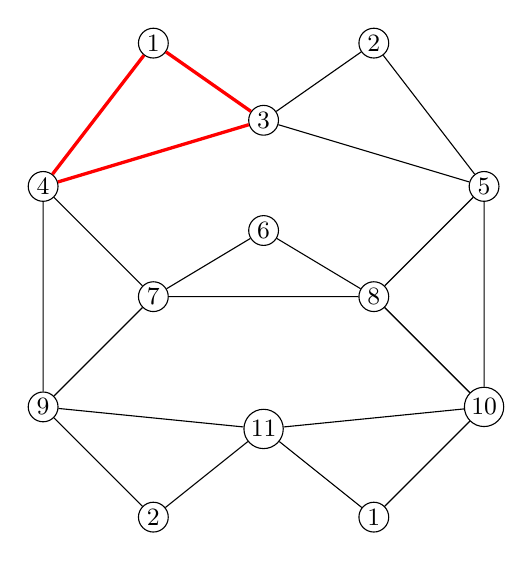
\begin{tikzpicture}[
  scale=1.4,
  vtx/.style={circle, draw, fill=white, inner sep=1.2pt, font=\small}
]

% --- Vertices (layout chosen to match the figure; 1 and 2 duplicated at bottom) ---
\node[vtx] (v1t)  at (-1,  2.5) {1};
\node[vtx] (v2t)  at ( 1,  2.5) {2};
\node[vtx] (v3)   at ( 0,  1.8) {3};

\node[vtx] (v4)   at (-2,  1.2) {4};
\node[vtx] (v5)   at ( 2,  1.2) {5};

\node[vtx] (v6)   at ( 0,  0.8) {6};
\node[vtx] (v7)   at (-1,  0.2) {7};
\node[vtx] (v8)   at ( 1,  0.2) {8};

\node[vtx] (v9)   at (-2, -0.8) {9};
\node[vtx] (v10)  at ( 2, -0.8) {10};
\node[vtx] (v11)  at ( 0, -1.0) {11};

\node[vtx] (v2b)  at (-1, -1.8) {2}; % duplicate of vertex 2
\node[vtx] (v1b)  at ( 1, -1.8) {1}; % duplicate of vertex 1

% --- Triangles (closed with -- cycle). Triangle 1 edges in red ---
\draw[very thick, red] (v1t) -- (v3) -- (v4) -- cycle;     % (1,1,3,4)
\draw                    (v2t) -- (v3) -- (v5) -- cycle;   % (2,2,3,5)
\draw                    (v4)  -- (v7) -- (v9) -- cycle;   % (3,4,7,9)
\draw                    (v5)  -- (v8) -- (v10) -- cycle;
\draw                    (v6)  -- (v7) -- (v8) -- cycle;   % (5,6,7,8)
\draw                    (v2b) -- (v9) -- (v11) -- cycle;  % (6,2,9,10)
\draw                    (v1b) -- (v10) -- (v11) -- cycle; % (7,1,10,11)

% --- Optional helper edges to match the frame/diagonals in the figure ---

\draw[very thick, red] (v1t) -- (v4);
\draw (v2b) -- (v11); 
\draw (v4) -- (v9);
\draw (v5) -- (v10);
\draw (v8) -- (v10);
\draw (v6) -- (v8);
\draw (v2t) -- (v5);
\draw (v1b) -- (v11);

\end{tikzpicture}
\caption{A triangular graph with 11 vertices.}
\label{F:triangular graph}
\end{figure}


Fix a triangular graph $\SG = (G, R)$. Let $\SF_G$ be the class of all real-valued functions whose domain is a triangle of $\SG$, i.e.,
\[
\SF_G = \{ f\colon A \to \BR \colon A \subseteq G \text{ is a triangle} \}.
\]

We define the binary relation $E$ on $\SF_G$ as follows. Given $f,g$ in $\SF_G$, we have $E(f,g)$ if and only if at least one of the following conditions is satisfied:

\begin{enumerate}[i)]

\item\label{D:graph equiv 1}
$f = g$; i.e., $\dom(f)=\dom(g)$ and $f(x)=g(x)$ for all $x\in\dom(f)$.

\item\label{D:graph equiv 2}
There exists $a\in \dom(f) \cap \dom(g)$ such that $f(a) = g(a)$, and every other element in $\dom(f)$ or $ \dom(g)$ is mapped to the same output. That is, \[
\dom(f)=\{a,b,c\} \quad \text{and} \quad  \dom(g)=\{a,b',c'\}
\]
such that $f(a)=g(a)$ and $f(b)=f(c)=g(b')=g(c')$.


\item\label{D:graph equiv 3}
$f(x)=g(y)$ for all $x\in\dom(f)$ and all $y\in\dom(g)$. In other words, $f$ and $g$ are both constant functions with the same constant value, and their domains are allowed to differ.

\end{enumerate}



\begin{claim}\label{C:E is equivalence relation} For a fixed $\SF_G$, the binary relation $E$ defined above is an equivalence relation.
\end{claim}


\begin{proof}[Proof of claim \ref{C:E is equivalence relation}] We will show that $E$ is reflexive, symmetric, and transitive.

\begin{enumerate}
\item[(Reflexivity)] Let $f\in\SF_G$. Then $f=f$, so $E(f,f)$ holds by i).

\item[(Symmetry)] Let $f,g\in\SF_G$ and suppose $E(f,g)$. That is, one of i), ii), or iii) holds for $f$ and $g$.

If i) holds, then $f=g$. This also means $g=f$, so $E(g,f)$ holds by i).

If ii) holds, then let $\dom(f)=\{a,b,c\}$ and $\dom(g)=\{a,b',c'\}$ such that $f(a)=g(a)$ and $f(b)=f(c)=g(b')=g(c')$. Since the equality relation ($=$) is symmetric, this gives us $E(g,f)$ by ii).

If iii) holds, then $f(x)=g(y)$ for any $x\in\dom(f)$ and any $y\in\dom(g)$. Again, $=$ is symmetric, so we have $E(g,f)$ by iii).

\item[(Transitivity)] Let $f,g,h\in\SF_G$ and suppose $E(f,g)$ and $E(g,h)$. In principle this gives us nine possibilities for which of i)-iii) are satisfied by $f,g$ and $g,h$. However, if $E(f,g)$ holds by i), then $E(f,h)$ holds in the same way that $E(g,h)$ holds: i), ii), or iii). The same is true when $E(g,h)$ holds by i). This shortens our list of possibilities to four, which we prove below.

\begin{enumerate}[(1)]

\item Suppose $E(f,g)$ and $E(g,h)$ hold by satisfying condition ii). Then we may express the domains of $f$ and $g$ by
\[
\dom(f)=\{a,b,c\} \quad \text{and} \quad \dom(g)=\{a,b',c'\}
\]
where $f(a)=g(a)$ and $f(b)=f(c)=g(b')=g(c')$. By condition ii), the domain of $h$ has one element in common with the domain of $g$, which could be either $a$, $b'$, or $c'$. If $a$ is the common element, then let us express the domain of $h$ by
\[
\dom(h)=\{a,b'',c''\}.
\]
Then $g(a)=h(a)$, and $g(b')=g(c')=h(b'')=h(c'')$. Since the $=$ relation is transitive, we have that ii) holds for $E(f,h)$.

If $b'$ is the common element, then let us express the domain of $h$ by
\[
\dom(h)=\{a'',b',c''\}
\]
where $g(b')=h(b')$, and $g(a)=g(c')=h(a'')=h(c'')$. But we already have that $g(c')=g(b')$ from $E(f,g)$, so now we see that 
\[
g(a)=g(b') = g(c') =h(a'')=h(b)=h(c'').
\]
Indeed, $f$, $g$, and $h$ are all constant functions with the same constant value. Thus $E(f,h)$ is satisfied by condition iii).

If $c'$ is the common element, then, by a similar argument, $E(f,h)$ is satisfied by iii).

\item Suppose both $E(f,g)$ and $E(g,h)$ hold by iii). Then $f$, $g$, and $h$ are all constant functions with the same constant value, so $E(f,h)$ by iii).

\item Suppose $E(f,g)$ holds by ii) and $E(g,h)$ holds by iii). Then $f(a)=g(a)$ and $f(b)=f(c)=g(b')=g(c')$. But, since $g$ is a constant function, both $f$ and $h$ are also constant functions with the same constant value, meaning $E(f,h)$ holds by iii).

\item Suppose $E(f,g)$ holds by iii) and $E(g,h)$ holds by ii). Then, by a similar argument as above, $E(f,h)$ is satisfied by iii).
\end{enumerate}
\end{enumerate}
\end{proof}


We will see that the equivalence classes of $E$ over the set $\SF_G$ act as ``observables" in a partial algebra (Definition~\ref{D:partial algebra}), given some natural interpretations of the relations and operations $\com$, $+$, $\circ$, $\cdot$, and $\mathbb{1}$. The rest of this section will be dedicated to defining these interpretations for a fixed graph and showing that the structure does indeed satisfy the properties of a partial algebra.

\begin{definition}\label{D:graph observables}
Fix a triangular graph $\SG=(G,R)$. Let $Q_{\SG}$ be the set of equivalence classes in $\SF_G$ over the relation $E$. We call the elements of $Q_{\SG}$ the \emph{observables} of $\SG$.
\end{definition}

Note: We use the term ``observables" because, eventually, we will define a correspondence between physically observable quantities and the mathematical elements of a partial algebra. The ``observables" of a (triangular) graph have no physical meaning; these graphs serve only as ``non-physical''examples of partial algebras to demonstrate their properties.

We now introduce a partial algebra structure on the set $Q_{\SG}$ of observables of a triangular graph $\SG$. We should denote this structure as $\mathfrak{Q}=(Q_{\SG},\com^{\mathfrak{Q}},+^{\mathfrak{Q}},\circ^{\mathfrak{Q}},\cdot^{\mathfrak{Q}},\mathbb{1}^{\mathfrak{Q}})$. To ease the notation, when this does not lead to confusion, we shall omit the superscripts from the relations and functions for the remainder of this section.

We start by defining a commeasurability relation $\com$ on $Q_{\SG}$. We will say that two observables $q_1, q_2\in Q_{\SG}$ are commeasurable if there exist functions $f_1\in q_1$ and $f_2\in q_2$ such that
\begin{align*}
\dom(f_1) = \dom(f_2).
\end{align*}

We now define the algebra operations of $\mathfrak{Q}$. Fix $q_1, q_2\in Q_{\SG}$ and 
 $f_1\in q_1$ and $f_2\in q_2$ such that $\dom(f_1) = \dom(f_2)$. Let $\lambda$ be a fixed real number. The sum and product of commeasurable observables are defined naturally as follows (where $+^{\BR}$ and $\cdot^{\BR}$ are the usual addition and multiplication of real numbers, respectively):

\begin{itemize}

\item 
$q_1 + q_2$ is the equivalence class of functions $f_1 + f_2$ defined by $(f_1+f_2)(x)=f_1(x)+^{\BR}f_2(x)$ for all $x\in\dom(f_1)$,

\item 
$q_1 \circ q_2$ is the equivalence class of functions $f_1 \circ f_2$ defined by $(f_1\circ f_2)(x)=f_1(x)\cdot^{\BR} f_2(x)$ for all $x\in\dom(f_1)$,


\item
$\lambda\cdot q_1$ is the equivalence class of functions $\lambda\cdot f_1$ defined by $(\lambda\cdot f_1)(x)=\lambda\cdot^{\BR}f_1(x)$ for all $x\in\dom(f_1)$.
\end{itemize}

We must show that these operations are well-defined; that is, the equivalence classes $q_1+q_2$, $q_1\circ q_2$, and $\lambda\cdot q_1$ do not depend on the choice of representatives $f_1\in q_1$ and $f_2\in q_2$. These proofs are tedious, similarly to claim $\ref{C:E is equivalence relation}$, but wegive the full details are below.

\begin{proof}[Proof that $+$ and $\circ$ are well-defined on $Q_{\SG}$] The proofs for $+$ and for $\circ$ are identical. Thus, we will present only the former. 

By definition of commeasurability, let $f_1,g_1\in q_1$ and $f_2,g_2\in q_2$ such that
\begin{align*}
\dom(f_1)&=\dom(f_2)=\{a,b,c\},\quad\text{and}\\
\dom(g_1)&=\dom(g_2)=\{a',b',c'\}.
\end{align*}

For simplicity, define $\dom(f)\coloneq\{a,b,c\}$ and $\dom(g)\coloneq\{a',b',c'\}$.

Note that $a,b,$ and $c$ are distinct, and likewise for $a',b',$ and $c'$ because the domains must be triangles in $\SG$. However, it is possible in general for an element in $\dom(f)$ to equal an element in $\dom(g)$.

We must show that $[f_1+f_2]=[g_1+g_2]$, or, in other words, that $E(f_1+ f_2,g_1+ g_2)$. We will prove this for each case of when $E(f_1,g_1)$ and $E(f_2,g_2)$ hold by i), ii), or iii).

\begin{enumerate}[(1)]

\item We first consider the case where $E(f_1,g_1)$ or $E(f_2,g_2)$ holds by i). Without loss of generality, suppose that $E(f_1,g_1)$ holds by i) (and let $E(f_2,g_2)$ hold by i), ii), or iii)). Thus $\dom(f_1)=\dom(g_1)=\{a,b,c\}$ and, for any $x\in\{a,b,c\}$, we have $f_1(x)=g_1(x)$. Similarly, since $E(f_2,g_2)$ holds, we have $f_2(x)=g_2(x)$ for any $x\in\{a,b,c\}$. Combining these pieces of information, we get that, for any $x\in\dom(f)=\dom(f_1+f_2)=\dom(g_1+g_2)$, we have
\begin{align*}
(f_1+f_2)(x)=f_1(x)+^{\BR}f_2(x)=g_1(x)+^{\BR}g_2(x)=(g_1+g_2)(x).
\end{align*}
By definition, $E(f_1+f_2,g_1+g_2)$ holds by i). We now consider the cases where neither $E(f_1,g_1)$ nor $E(f_2,g_2)$ hold by i).

\item Suppose $E(f_1,g_1)$ and $E(f_2,g_2)$ both hold by ii). Suppose the common element between $\dom(f_1)$ and $\dom(g_1)$ is different from the common element between $\dom(f_2)$ and $\dom(g_2)$, say $a\in\dom(f_1)\cap\dom(g_1)$ and $b\in\dom(f_2)\cap\dom(g_2)$. However, $\dom(f_1)\cap\dom(g_1)=\dom(f_2)\cap\dom(g_2)$ because $\dom(f_1)=\dom(f_2)$ and likewise for $g_1$ and $g_2$. By the definition of triangular graph, for any triangle that includes $a$ and $b$ (e.g., $\dom(f)$ and $\dom(g)$), there exists exactly one element also in that triangle. Therefore $c=c'\in\dom(f)\cap\dom(g)$. We see that $\dom(f)=\dom(g)=\{a,b,c\}$, and we use the same argument as in the case where i) held.

Suppose instead that the element in common between $\dom(f_1)$ and $\dom(g_1)$ is the same element that is in common between $\dom(f_2)$ and $\dom(g_2)$. Call this element $a$ in either case, and let $\dom(f)=\{a,b,c\}$ and $\dom(g)=\{a,b',c'\}$. Now we have the following equations by ii):
\begin{align*}
&f_1(a)=g_1(a),\quad f_1(b)=f_1(c)=g_1(b')=g_1(c'),\quad\text{and}\\
&f_2(a)=g_2(a),\quad f_2(b)=f_2(c)=g_2(b')=g_2(c').
\end{align*}
Now we can see that the functions $f_1+f_2$ and $g_1+g_2$ act similarly to one another on their domains:
\begin{align*}
&(f_1+f_2)(a)=f_1(a)+^{\BR}f_2(a)=g_1(a)+^{\BR}g_2(a)=(g_1+g_2)(a),\quad\text{and similarly,}\\
&(f_1+f_2)(b)=(f_1+f_2)(c)=(g_1+g_2)(b')=(g_1+g_2)(c').
\end{align*}

In fact, this shows that $E(f_1+f_2,g_1+g_2)$ holds by ii).

\item Suppose $E(f_1,g_1)$ and $E(f_2,g_2)$ both hold by iii). Let $\mu_1\in\BR$ be the constant value of $f_1$ and $g_1$, and let $\mu_2\in\BR$ be the constant value of $f_2$ and $g_2$. Then $(f_1+f_2)(x)=\mu_1+^{\BR}\mu_2$ for all $x\in\dom(f)$, and $(g_1+g_2)(x')=\mu_1+^{\BR}\mu_2$ for all $x'\in\dom(g)$. So $E(f_1+f_2,g_1+g_2)$ holds by iii) since both functions have the constant value $\mu_1+^{\BR}\mu_2$.

\item Suppose $E(f_1,g_1)$ holds by ii) with common domain element $a$ between $\dom(f)$ and $\dom(g)$, and suppose $E(f_2,g_2)$ holds by iii) with constant value $\mu_2\in\BR$. Then 
\begin{align*}
f_1(a)=g_1(a),\quad f_1(b)=f_1(c)=g_1(b')=g_1(c'),
\end{align*}
and for all $x\in\dom(f)$ and all $x'\in\dom(g)$,
\begin{align*}
f_2(x)=\mu_2, \quad g_2(x')=\mu_2.
\end{align*}
Now we see that
\begin{align*}
&(f_1+f_2)(a)=f_1(a)+^{\BR}\mu_2=g_1(a)+^{\BR}\mu_2=(g_1+g_2)(a)\quad\text{and, similarly,}\\
&(f_1+f_2)(b)=(f_1+f_2)(c)=(g_1+g_2)(b')=(g_1+g_2)(c').
\end{align*}
Thus, $E(f_1+f_2,g_1+g_2)$ holds by ii).

\item Suppose $E(f_1,g_1)$ holds by iii) with constant value $\mu_1\in\BR$, and suppose $E(f_2,g_2)$ holds by ii) with common domain element $a$  between $\dom(f)$ and $\dom(g)$. By an analogous argument as above, $E(f_1+f_2,g_1+g_2)$ holds by ii).
\end{enumerate}
\end{proof}

\begin{proof}[Proof that $\cdot$ is well-defined on $\BR\times Q_{\SG}$] Let $\lambda\in\BR$ and $q\in Q_{\SG}$ be fixed. Let $f,g\in q$; that is, $E(f,g)$. We analyze three cases for this relation:

\begin{enumerate}[(1)]
\item Suppose $E(f,g)$ holds by i). Then $f=g$ so $\lambda\cdot f=\lambda\cdot g$ is immediate, and we conclude that $E(\lambda\cdot f,\lambda\cdot g)$ holds by i).

\item Suppose $E(f,g)$ holds by ii) with common domain element $a\in\dom(f)\cap\dom(g)$. Without loss of generality, let $\dom(f)=\{a,b,c\}$ and $\dom(g)=\{a,b',c'\}$. We have the following relationship between $f$ and $g$ by ii):
\begin{align*}
f(a)=g(a),\quad f(b)=f(c)=g(b')=g(c').
\end{align*}
Now we can see how $\lambda\cdot f$ and $\lambda\cdot g$ are related by $E$:
\begin{align*}
&(\lambda\cdot f)(a)=\lambda\cdot^{\BR}f(a)=\lambda\cdot^{\BR}g(a)=(\lambda\cdot g)(a),\quad\text{and}\\
&(\lambda\cdot f)(b)=(\lambda\cdot f)(c)=(\lambda\cdot g)(b')=(\lambda\cdot g)(c').
\end{align*}
Thus, $E(\lambda\cdot f,\lambda\cdot g)$ holds by ii).

\item Suppose $E(f_1,g_1)$ holds by iii) with constant value $\mu\in\BR$. Then for all $x\in\dom(f)$ and all $x'\in\dom(g)$,
\begin{align*}
(\lambda\cdot f)(x)=\lambda\cdot^{\BR}f(x)=\lambda\cdot^{\BR}\mu=\lambda\cdot g(x')=(\lambda\cdot g)(x').
\end{align*}
Therefore, $E(\lambda\cdot f,\lambda\cdot g)$ holds by iii) since both functions have the constant value $\lambda\cdot^{\BR}\mu$.
\end{enumerate}
\end{proof}

We define the element $\mathbb{1}$ to be the equivalence class associated with the functions in $\SF_G$ of constant value 1. Condition iii) for the equivalence relation $E$ ensures that all such functions belong to the same equivalence class. Let $q$ be any observable in $Q_{\SG}$. There exists a representative $f\in q$ with a domain $\dom(f)$, and the constant function with value 1 defined on $\dom(f)$ will be in the equivalence class $\mathbb{1}$. Therefore, $q\com\mathbb{1}$.

We will now show that the commeasurability relation is preserved under the operations $+$, $\circ$, and $\cdot$.

\begin{proof}[Proof that $\mathfrak{Q}$ satisfies property 2) of Definition~\ref{D:partial algebra}] Let $q_1,q_2,q_3$ be observables that are pairwise commeasurable. Since we have three commeasurability relations up to symmetry ($q_1\com q_2$, $q_2\com q_3$, and $q_3\com q_1$), for any two commeasurable observables, there exist pairs of functions with a shared domain. We will call these functions $f_1,f_2,g_2,g_3,h_1,$ and $h_3$ with the following properties (summarized in the table below). A subscript of $i$ indicates that the function is in the equivalence class $q_i$. The letter of the function ($f,g,h$) indicates the domain it is defined on. For instance, $f_1$ and $f_2$ share a domain, abbreviated simply as $\dom(f)$. In the table below, each column indicates equivalence class membership, and each row indicates a common domain.

\[\begin{array}{|c|c||c|c|c|}
\hline \text{Commeasurability relation} & \text{Domain} & q_1 & q_2 & q_3 \\ \hline\hline
q_1\com q_2 & \dom(f) & f_1 & f_2 & \cellcolor{lightgray} \\ \hline
q_2\com q_3 & \dom(g) & \cellcolor{lightgray} & g_2 & g_3\\ \hline
q_1\com q_3 & \dom(h) & h_1 & \cellcolor{lightgray} & h_3 \\ \hline
\end{array}\]

We will show that $(q_1+q_2)\com q_3$. We have many possible cases to treat because $E(f_1,h_1)$, $E(f_2,g_2)$, and $E(g_3,h_3)$ can each hold by any one of i), ii), or iii). We can shorten these 27 cases to the following seven, some of which use redundant arguments:

\begin{enumerate}
\item Suppose that $E(f_1,h_1)$ holds by i). That is, $f_1=h_1$, and $\dom(f)=\dom(h)$. Therefore the functions $f_1+f_2\in q_1+q_2$ and $h_3\in q_3$ have the same domain, meaning $(q_1+q_2)\com q_3$.

\item Suppose that $E(f_2,g_2)$ holds by i). That is, $f_2=g_2$, and $\dom(f)=\dom(g)$. Then, the functions $f_1+f_2\in q_1+q_2$ and $g_3\in q_3$ have the same domain, meaning $(q_1+q_2)\com q_3$.

\item Suppose that $E(g_3,h_3)$ holds by i). That is, $g_3=h_3$, and $\dom(g)=\dom(h)$. Then, the function $h_1+g_2\in q_1+q_2$ is defined on that domain, so $(q_1+q_2)\com q_3$.

Henceforth, we assume that none of the functions are related (under $E$) by i).

\item Suppose that $E(f_1,h_1)$ holds by iii). Let the constant value of the functions $f_1$ and $h_1$ be denoted $\mu_1\in\BR$. Now the function $\mu_1+g_2$ defined for all $x\in\dom(g)$ by
\begin{align*}
(\mu_1+g_2)(x)=\mu_1+^{\BR}g_2(x)
\end{align*}
is in the equivalence class $q_1+q_2$. Since it shares its domain with $g_3\in q_3$, we have $(q_1+q_2)\com q_3$.

\item Suppose that $E(f_2,g_2)$ holds by iii). Let the constant value of the functions $f_2$ and $g_2$ be denoted $\mu_2\in\BR$. Now the function $h_1+\mu_2$ defined for all $x\in\dom(h)$ by
\begin{align*}
(h_1+\mu_2)(x)=h_1(x)+^{\BR}\mu_2
\end{align*}
is in the equivalence class $q_1+q_2$. Since it shares its domain with $h_3\in q_3$, we have $(q_1+q_2)\com q_3$.

\item Suppose that $E(g_3,h_3)$ holds by iii). Let the constant value of the functions $g_3$ and $h_3$ be denoted $\mu_3\in\BR$. There exists a function $f_3\in q_3$ defined for all $x\in\dom(f)$ by $f_3(x)=\mu_3$, and since this shares its domain with $f_1+f_2\in q_1+q_2$, we have $(q_1+q_2)\com q_3$.

Henceforth, we assume that none of the functions are related (under $E$) by iii).

\item Our final case is where $E(f_1,h_1)$, $E(f_2,g_2)$, and $E(g_3,h_3)$ all hold by ii). This means that each pairwise intersection of $\dom(f),\dom(g),$ and $\dom(h)$ contains one element. If any intersection contains two elements, then by the triangular graph property (because each domain is a triangle), the intersection contains all three elements, meaning the two domains are equal. If any two of the domains are equal, then we use the same arguments as in cases (1)-(3) to show that $(q_1+q_2)\com q_3$.

Without loss of generality, we can write the domains $\dom(f)$ and $\dom(g)$ as the following (where each element is distinct):
\begin{align*}
\dom(f)=\{a,b,c\},\quad\dom(g)=\{a,b',c'\}
\end{align*}
Now $\dom(h)$ must share a common element with both $\dom(f)$ and $\dom(g)$. If $a\notin\dom(h)$, then without loss of generality suppose $b,b'\in\dom(h)$. Then $b$ is adjacent to $b'$ since $\dom(h)$ must be a triangle. Since both $b$ and $b'$ are each already adjacent to $a$, the triangle $\dom(h)$ must contain $a$ by the triangle property of the graph $\SG$. So in any case, we have $a\in\dom(h)$. Now because the common element between $\dom(g)$ and $\dom(h)$ is $a$, we have $g_3(b')=g_3(c')$. We can define a function $f_3$ on $\dom(f)$ by
\begin{align*}
f_3(a)=g_3(a),\quad f_3(b)=f_3(c)=g_3(b')=g_3(c').
\end{align*}
This function $f_3$ has the property that $E(f_3,g_3)$ by ii), so $f_3\in q_3$. This function shares a domain with $f_1+f_2\in q_1+q_2$, so $(q_1+q_2)\com q_3$.
\end{enumerate}

The preceding argument, with $+,+^{\BR}$ is replaced with $\circ,\cdot^{\BR}$, respectively can be repeated to show that $(q_1\circ q_2)\com q_3$.

Now we will show that $(\lambda\cdot q_1)\com q_2$ for a fixed real number $\lambda$. Since $q_1\com q_2$, there exist functions $f_1\in q_1$ and $f_2\in q_2$ so that $\dom(f_1)=\dom(f_2)$. We define the function $\lambda\cdot f_1$ by $(\lambda\cdot f_1)(x)=\lambda\cdot^{\BR}f_1(x)$ for all $x\in\dom(f_1)$. Since $\lambda\cdot f_1$ shares its domain with $f_2$, we have $(\lambda\cdot q_1)\com q_2$.
\end{proof}

We will now show that any three pairwise commeasurable observables $q_1,q_2,q_3\in Q_{\SG}$ generate (through addition, multiplication, and scalar multiplication) a commutative algebra over $\BR$.


%The following proof is incomplete
\begin{proof}[Proof that $\mathfrak{Q}$ satisfies property 3) of Definition~\ref{D:partial algebra}] 


\end{proof}






\subsection{Polynomials in partial algebras}


In this section, we define the notion of a ``polynomial'' and extend the idea to apply to partial algebras. We will use $P_n$ (for some $n\in\mathbb{N}$) to denote the set of formal expressions using the symbols $\circone,x_1,x_2,\ldots,x_n$, a symbol for each real number (for which we use the letters $\lambda,\mu$, etc), the symbols $\oplus,\otimes,\odot$, parenthesis $(,),[,]$, etc (for clarity) that result from applying  the following rules of formation finitely many times:

\begin{itemize}
\item $\circone$ is in $P_n$.

\item If $i\in\{1,2,\ldots,n\}$, then $x_i$ is in $P_n$.

\item If $\phi$ is in $P_n$ and $\lambda\in\BR$, then $\lambda\odot\phi$ is in $P_n$.

\item If $\phi,\psi$ are in $P_n$, then $\phi\oplus\psi$ is in $P_n$ and $\phi\otimes\psi$ is in $P_n$.
\end{itemize}

\begin{examples}\phantom{a}

\begin{enumerate}
\item The expression $x_1$ is in $P_n$ for any $n\geq1$.

\item The expression $x_1\oplus x_2$ is in $P_n$ for any $n\geq 2$.

\item The expression $(5\odot\circone)\oplus(x_1\otimes x_3)$ is in $P_n$ for any $n\geq3$.
\end{enumerate}
\end{examples}

Now we define the notion of interpreting these expressions in a partial algebra.

\begin{definition}
Fix a partial algebra $\FA=(A\com,+,\circ,\cdot,\mathbb{1})$, and let $\phi$ belong to $P_n$ (for a fixed $n\in\mathbb{N}$). We define:
\begin{itemize}
\item
A subset $D_{\phi,n}^{\FA}\subseteq A^n$ called  the \emph{domain} of $\phi$, and 
\item
A map $\phi_n^{\FA}:D_{\phi,n}^{\FA}\to A$ called the \emph{evaluation map} of $\phi$
\end{itemize}
 recursively as follows:
 
\begin{enumerate}[i)]

\item If $\phi$ is the expression $\circone$, then $D_{\phi,n}^{\FA}=A^n$ and $\phi_n^{\FA}(\bar{q})=\mathbb{1}$ for all $\bar{q}\in A^n$.

\item If $\phi$ is the expression $x_i$ where $i\in\{1,2,\ldots,n\}$, then $D_{\phi,n}^{\FA}=A^n$ and if $\bar{q}\in A^n$, then $\phi_n^{\FA}(\bar{q})=q_i$.

\item If $\phi$ is the expression $\lambda\odot\psi$ where $\lambda\in\BR$ and $\psi$ is in $P_n$, then $D_{\phi,n}^{\FA}=D_{\psi,n}^{\FA}$ and if $\bar{q}\in D_{\psi,n}^{\FA}$, then $\phi_n^{\FA}(\bar{q})=\lambda\cdot\psi_n^{\FA}(\bar{q})$.

\item If $\phi$ is the expression $\psi\oplus\sigma$ where $\psi$ and $\sigma$ are in $P_n$,  then 
\[
D_{\phi,n}^{\FA}=\{\bar{q}\in D_{\psi,n}^{\FA}\cap D_{\sigma,n}^{\FA}\colon\psi_n^{\FA}(\bar{q})\com\sigma_n^{\FA}(\bar{q})\}
\]
and if $\bar{q}\in D_{\phi,n}^{\FA}$, then $\phi_n^{\FA}(\bar{q})=\psi_n^{\FA}(\bar{q})+\sigma_n^{\FA}(\bar{q})$.

\item If $\phi$ is the expression $\psi\otimes\sigma$ where $\psi$ and $\sigma$ are in $P_n$,  then 
\[
D_{\phi,n}^{\FA}=\{\bar{q}\in D_{\psi,n}^{\FA}\cap D_{\sigma,n}^{\FA}\colon\psi_n^{\FA}(\bar{q})\com\sigma_n^{\FA}(\bar{q})\}
\]
and if $\bar{q}\in D_{\phi,n}^{\FA}$, then $\phi_n^{\FA}(\bar{q})=\psi_n^{\FA}(\bar{q})\circ\sigma_n^{\FA}(\bar{q})$.
\end{enumerate}
\end{definition}

Now we define a notion of when two expressions in $P_n$ are equal in a partial algebra.

\begin{definition}
Fix a partial algebra $\FA=(A\com,+,\circ,\cdot,\mathbb{1})$, and let $\phi,\psi$ be expressions in $P_n$. We call an equation of the form
\[
\phi=\psi 
\]
an \emph{identity} in $\FA$ if and only if, for all $\bar{q}\in D_{\psi,n}\cap D_{\sigma,n}$, the following implication holds:
\begin{center}
If $\phi_n^{\FA}(\bar{q})\com\psi_n^{\FA}(\bar{q})$, then  $\phi_n^{\FA}(\bar{q})=\psi_n^{\FA}(\bar{q})$.
\end{center}
\end{definition}

\begin{examples} Fix a partial algebra $\FA=(A,\com,+,\circ,\cdot,\mathbb{1})$.
\begin{enumerate}[(1)]
\item
Let $n$ be any natural number, and let $i,j\in\{1,2,\ldots,n\}$. The equation $x_i\oplus x_j=x_j\oplus x_i$ is an identity in $\FA$.
\begin{proof}
Let $\phi$ be the expression $x_i\oplus x_j$, and let $\psi$ be the expression $x_j\oplus x_i$, so that $\phi,\psi\in P_n$. The domain of $\phi$ is the set of all $\bar{q}=(q_1,q_2,\ldots,q_n)\in A^n$ such that $q_i\com q_j$, and the domain of $\psi$ consists of all $\bar{q}\in A^n$ such that $q_j\com q_i$. Since $\venus$ is symmetric, we see that
\[
D_{\phi,n}^{\FA}=D_{\psi,n}^{\FA}=\{(q_1,q_2,\ldots,q_n)\in A^n\,\colon\,q_i\com q_j\}=D_{\phi,n}^{\FA}\cap D_{\psi,n}^{\FA}.
\]


Let $\bar{q}$ be any element of $D_{\phi,n}^{\FA}\cap D_{\psi,n}^{\FA}$. Then $q_i\com q_j$, so by property 3) of Definition~\ref{D:partial algebra}, $q_i$ and $q_j$ generate a commutative algebra. Hence,
\[
\phi_n^{\FA}(\bar{q}) = q_i+q_j = q_j+q_i = \psi_n^{\FA}(\bar{q}).
\]
\end{proof}

\item
Let $n$ be any natural number, and let $i,j,k\in\{1,2,\ldots,n\}$. The equation $x_i\oplus(x_j\oplus x_k)=(x_i\oplus x_j)\oplus x_k$ is a an identity in $\FA$.
\begin{proof}
Let $\phi$ be the expression $x_i\oplus(x_j\oplus x_k)$ and let $\psi$ be the expression $(x_i\oplus x_j)\oplus x_k$. Let $\bar{q}$ be shorthand for $(q_1,q_2,\ldots,q_n)$. The domain of $\phi$ is the set of all $\bar{q}\in A^n$ such that $q_j\com q_k$ and $q_i\com(q_j+q_k)$. The domain of $\psi$ is the set of all $\bar{q}\in A^n$ such that $q_i\com q_j$ and $(q_i+q_j)\com q_k$.
\begin{align*}
D_{\phi,n}^{\FA}&=\{\bar{q}\in A^n\,\colon\,q_j\com q_k\text{ and } q_i\com(q_j+q_k)\}\\
D_{\psi,n}^{\FA}&=\{\bar{q}\in A^n\,\colon\,q_i\com q_j\text{ and }(q_i+q_j)\com q_k\}\\
D_{\phi,n}^{\FA}\cap D_{\psi,n}^{\FA}&=\left\{\bar{q}\in A^n\,\colon\,q_i\com q_j,\,q_j\com q_k,q_i\com(q_j+q_k),\text{ and }(q_i+q_j)\com q_k\right\}
\end{align*}
Note that $q_i\com q_j$ implies that $q_i\com(-1\cdot q_j)$ by property 2) of the definition of a partial algebra (Definition~\ref{D:partial algebra}). Also, $q_j\com q_k$ implies that $q_j\com(q_j+q_k)$ and $-1\cdot q_j\com(q_j+q_k)$. Since we also have that $q_i\com(q_j+q_k)$, we conclude that $q_i,(-1\cdot q_j),$ and $(q_j+q_k)$ are pairwise commeasurable. Commeasurability of these elements is preserved under $+$, so we have that $q_i\com((-1\cdot q_j)+q_j+q_k)$, or simply $q_i\com q_k$. Therefore, whenever $\bar{q}\in D_{\phi,n}^{\FA}\cap D_{\psi,n}^{\FA}$, we have that $q_i,q_j,q_k$ are pairwise commeasurable. By property 2) of the definition of a partial algebra, this means that for any $\bar{q}$ in both the domain of $\phi$ and of $\psi$, we have
\begin{align*}
q_i+(q_j+q_k)&\com(q_i+q_j)+q_k,\quad \text{or alternatively},\\
\phi_n^{\FA}(\bar{q})&\com\psi_n^{\FA}(\bar{q}).
\end{align*}
Furthermore, property 3) of the definition of a partial algebra ensures that $q_i+(q_j+q_k)=(q_i+q_j)+q_k$ for all such $\bar{q}$ since addition is associative in any commutative algebra. Hence, $\phi=\psi$ is an identity in $\FA$.
\end{proof}

\item
\textbf{Non-example}: The equation $(x_1\oplus x_2)\oplus(x_3\oplus x_4)=(x_1\oplus x_4)\oplus(x_2\oplus x_3)$ is \textbf{not} an identity for every partial algebra (where $n\geq4$). We will construct a partial algebra using observables on a graph as a counterexample. Define $\phi$ to be the expression $(x_1\oplus x_2)\oplus(x_3\oplus x_4)$, and $\psi$ the expression $(x_1\oplus x_4)\oplus(x_2\oplus x_3)$.

Note: The key reason why this equation doesn't hold in all partial algebras, whereas the prior equations do, has to do with commeasurability. We will see that the allowable tuples of elements of the partial algebra (usually called $\bar{q}$) are not quite restricted enough to ensure equality between $\phi$ and $\psi$. For any such tuple $(q_1,q_2,\ldots,q_n)$ in the domain of both $\phi$ and $\psi$, it is ensured that $q_1\com q_2$ and that $q_1\com q_4$, but not that $q_1\com q_3$. We saw something similar in the associativity example, where $q_1\com q_3$ was not explicitly given by the definition of the domains. However, in that case it was possible to determine that $q_1\com q_3$ must hold anyway, regardless of the partial algebra. In the case of $\phi=\psi$, it is not possible to show that $q_1\com q_3$ for all partial algebras; in fact, it will not hold for our counterexample. Hence, it will be possible to add elements $q_1,q_2,q_3,$ and $q_4$ in different orders and obtain different values.

\begin{proof}
We will consider the 11-vertex, triangular graph $\SG=(G,R)$ shown in Figure~\ref{F:triangular graph} and the set of observables $Q_{\SG}$ on that graph. Let $\FQ=(Q_{\SG},\com,+,\circ,\cdot,\mathbb{1})$. We present four distinct real-valued functions $f_1,f_2,f_3,f_4\in\SF_G$ which are representatives of four equivalence classes (observables), which we will call $q_1,q_2,q_3,$ and $q_4$, respectively. For the sake of clarity and legibility, we will use a two-line notation for functions. For instance, if a function $f$ is defined on the vertices $v_1,v_3,$ and $v_4$ with values $a,b,c\in\BR$:
\begin{align*}
f(v_1)=a,\quad f(v_3)=b,\quad f(v_4)=c,
\end{align*}
then we write $f$ in the following form:
\begin{align*}
f=\begin{pmatrix}
v_1 & v_3 & v_4\\
a & b & c
\end{pmatrix}
\end{align*}
Note that we are not adopting the previous convention that functions with the same letter in their name have the same domain ($\dom(f_i)\ne\dom(f_j)$, in general). The proposed functions are the following:
\begin{align*}
f_1=\begin{pmatrix}
v_1 & v_3 & v_4\\
1 & 0 & 0
\end{pmatrix},\quad f_2=\begin{pmatrix}
v_1 & v_3 & v_4\\
0 & 1 & 0
\end{pmatrix},\\
f_3=\begin{pmatrix}
v_2 & v_3 & v_5\\
1 & 0 & 0
\end{pmatrix},\quad f_4=\begin{pmatrix}
v_2 & v_9 & v_{11}\\
0 & 0 & 1
\end{pmatrix}
\end{align*}
Now we can consider other functions $g_1,g_2,g_3,g_4$ that are in the equivalence classes $q_1,q_2,q_3,q_4$, respectively (because $E(f_i,g_i)$ holds by ii):
\begin{align*}
g_1=\begin{pmatrix}
v_1 & v_{10} & v_{11}\\
1 & 0 & 0
\end{pmatrix},\quad g_2=\begin{pmatrix}
v_2 & v_3 & v_5\\
0 & 1 & 0
\end{pmatrix},\\
g_3=\begin{pmatrix}
v_2 & v_9 & v_{11}\\
1 & 0 & 0
\end{pmatrix},\quad g_4=\begin{pmatrix}
v_1 & v_{10} & v_{11}\\
0 & 0 & 1
\end{pmatrix}
\end{align*}
Notice that the domains of these functions can tell us whether two observables $q_i$ and $q_j$ are commeasurable. For instance, we see that $q_1\com q_2$ since $\dom(f_1)=\dom(f_2)$, and $q_3\com q_4$ because $\dom(g_3)=\dom(f_4)$. By commeasurability, we are able to add some of these observables together by adding representative functions that share a domain (the $+$ below indicates function addition and should be considered part of the names of the functions).
\begin{align*}
f_1+f_2=\begin{pmatrix}
v_1 & v_3 & v_4\\
1 & 1 & 0
\end{pmatrix},\quad g_3+f_4=\begin{pmatrix}
v_2 & v_9 & v_{11}\\
1 & 0 & 1
\end{pmatrix},\\
g_1+g_4=\begin{pmatrix}
v_1 & v_{10} & v_{11}\\
1 & 0 & 1
\end{pmatrix},\quad g_2+f_3=\begin{pmatrix}
v_2 & v_3 & v_5\\
1 & 1 & 0
\end{pmatrix}
\end{align*}
These functions are members of the equivalence classes $q_1+q_2$, $q_3+q_4$, $q_1+q_4$, and $q_2+q_3$, respectively. Similarly to before, we can find other functions (which we name with the letter ``$h$'') in these equivalence classes that are related under $E$ by ii):
\begin{align*}
h_{1+2}=\begin{pmatrix}
v_4 & v_7 & v_9\\
0 & 1 & 1
\end{pmatrix},\quad h_{3+4}=\begin{pmatrix}
v_4 & v_7 & v_9\\
1 & 1 & 0
\end{pmatrix},\\
h_{1+4}=\begin{pmatrix}
v_5 & v_8 & v_{10}\\
1 & 1 & 0
\end{pmatrix},\quad h_{2+3}=\begin{pmatrix}
v_5 & v_8 & v_{10}\\
0 & 1 & 1
\end{pmatrix}
\end{align*}
Notice that $\dom(h_{1+2})=\dom(h_{3+4})$ and $\dom(h_{1+4})=\dom(h_{2+3})$, indicating respectively that $(q_1+q_2)\com(q_3+q_4)$ and $(q_1+q_4)\com(q_2+q_3)$. Adding these $h$ functions together, we get
\begin{align*}
h_{1+2}+h_{3+4}=\begin{pmatrix}
v_4 & v_7 & v_9\\
1 & 2 & 1
\end{pmatrix},\quad h_{1+4}+h_{2+3}=\begin{pmatrix}
v_5 & v_8 & v_{10}\\
1 & 2 & 1
\end{pmatrix}
\end{align*}
Finally, we examine two other functions that are equivalent to these, which we name with the letter ``$j$'' as follows:
\begin{align*}
j_{\phi}=\begin{pmatrix}
v_6 & v_7 & v_8\\
1 & 2 & 1
\end{pmatrix},\quad j_{\psi}=\begin{pmatrix}
v_6 & v_7 & v_8\\
1 & 1 & 2
\end{pmatrix}
\end{align*}
Since $\dom(j_{\phi})=\dom(j_{\psi})$, we see that $[(q_1+q_2)+(q_3+q_4)]\com[(q_1+q_4)+(q_2+q_3)]$, however these observables are not equal to one another since $j_{\phi}$ is not equivalent to $j_{\psi}$ by $E$. Ultimately, we have found an $n$-tuple $\bar{q}=(q_1,q_2,q_3,q_4,\circone,\circone,\ldots,\circone)\in A^n$ that is in both $D_{\phi,n}^{\FQ}$ and $D_{\psi,n}^{\FQ}$ such that $\phi_n^{\FQ}(\bar{q})\com\psi_n^{\FQ}(\bar{q})$ but $\phi_n^{\FQ}(\bar{q})\ne\psi_n^{\FQ}(\bar{q})$. This is the negation of the definition that $\phi=\psi$ is a $P_n$ partial polynomial identity, so we are done.
\end{proof}

\end{enumerate}
\end{examples}


\subsection{Partial Boolean algebras}
\begin{definition}\label{D:partial boolean algebra}
A \emph{partial Boolean algebra} (over the real numbers $\BR$) is a structure $\FB = (B, \com, \lor, \neg,\mathbb{0}, \mathbb{1})$, where
\begin{itemize}

\item
$B$ is a nonempty set called the \emph{domain} or \emph{universe} of $\FB$,

\item
$\venus$ is a binary relation on $B$ that is reflexive and symmetric,

\item
$\lor \colon \{ (q_1, q_2 ) \in B\times B \colon q_1 \com q_2 \} \to B  $ is a partial binary function on $B$,

\item
$\neg \colon B \to B $ is a unary operation on $B$, and

\item
$\mathbb{0}$ and $\mathbb{1}$ are elements of $B$,
\end{itemize}
satisfying the following properties:

\begin{enumerate}[(1)]

\item
For all $q\in B$, $q\com \mathbb{0}$ and $q \com \mathbb{1}$.

\item\label{P:pba com preserved}
If $q_1,q_2,q_3\in B$ are pairwise related by $\venus$, then
\[
(q_1 \lor q_2) \com q_3, \quad (\neg q_1) \com q_2.
\]

\item\label{P:pba boolean algebra}
If $q_1,q_2,q_3\in B$ are pairwise related by $\venus$, then the set generated by $q_1,q_2,$ and $q_3$ according to the operations $\lor$ and $\neg$ is a Boolean algebra (with $\mathbb{0}$ and $\mathbb{1}$ as the Boolean elements 0 and 1, respectively).

\end{enumerate}

\end{definition}

Given a partial Boolean algebra, we can define other familiar logical symbols as compositions of the operations $\lor$ and $\neg$. We define $\land,\to,\leftrightarrow$ in the usual way:
\begin{align*}
q_1\land q_2 &\coloneq\neg((\neg q_1)\lor(\neg q_2))\\
q_1\to q_2 &\coloneq(\neg q_1)\lor q_2\\
q_1\leftrightarrow q_2 &\coloneq(q_1\to q_2)\land(q_2\to q_1)
\end{align*}

\begin{definition}
A structure $\mathfrak{C}=(C,\lor,\neg,0,1)$ is a \emph{Boolean algebra} if the below properties are satisfied for all $x,y,z\in C$. For simplicity of notation, define $\land$ by $x\land y=\neg((\neg x)\lor(\neg y))$.
\begin{align*}
\text{(Commutativity)} &\quad x\lor y=y\lor x \qquad\text{and}\qquad x\land y=y\land x\\
%\text{(Associativity)} &\quad x\lor(y\lor z)=(x\lor y)\lor z \qquad\text{and}\qquad x\land(y\land z)=(x\land y)\land z\\
%\text{(Absorption)} &\quad x\lor(x\land y)=x \qquad\text{and}\qquad x\land(x\lor y)=x\\
\text{(Distributivity)} &\quad x\lor(y\land z)=(x\lor y)\land(x\lor z)\qquad\text{and}\\
&\quad x\land(y\lor z)=(x\land y)\lor(x\land z)\\
\text{(Identity Elements)} &\quad x\lor0=x \qquad\text{and}\qquad x\land1=x\\
\text{(Complementation)} &\quad x\land(\neg x)=0 \qquad\text{and}\qquad x\lor(\neg x)=1
\end{align*}
\end{definition}

\begin{remark}
Other features of a Boolean algebra, such as associativity and absorption, can be proven using just the four properties above.
\end{remark}


\begin{definition}
An element $a$ of a partial algebra $\FA=(A\com,+,\circ,\cdot,\mathbb{1})$ is \emph{idempotent} if $a\circ a=a$.
\end{definition}

\begin{remark}
Note that if $\FA=(A\com,+,\circ,\cdot,\mathbb{1})$ is a partial algebra, then $\mathbb{1}\circ\mathbb{1}=\mathbb{1}$ and
$0\cdot\mathbb{1}\circ0\cdot\mathbb{1}$ since
$\mathbb{1}\com\mathbb{1}$
and
$0\cdot\mathbb{1}\com0\cdot\mathbb{1}$. 
Hence,
$\mathbb{1}$ and
$0\cdot\mathbb{1}$ are idempotent elements of $\FA$.

\end{remark}


\begin{example}
Given a partial algebra $\FA=(A,\com^{\FA},+,\circ,\cdot,\mathbb{1}^{\FA})$, the idempotent elements of $\FA$ form a partial Boolean algebra; more precisely, if we define
\[
\FB=(B,\com^{\FB},\lor,\neg,\mathbb{0}^{\FB},\mathbb{1}^{\FB}),
\]
where
\begin{itemize}
\item
$B\subseteq A$ is the set of idempotent elements of $\FA$,

\item
$\com^{\FB}$ is the restriction of $\com^{\FA}$ to the domain $B\times B\subseteq A\times A$,

\item
$\lor$ is defined for all $(q_1,q_2)\in B\times B$ such that $q_1\com^{\FB}q_2$ by
\[
q_1\lor q_2=q_1+q_2+(-1\cdot(q_1\circ q_2)),
\]

\item
$\neg$ is defined for all $q\in B$ by $\neg q=\mathbb{1}^{\FA}+(-1\cdot q)$ (indeed, any $q\in B$ is commeasurable with $\mathbb{1}$),

\item
$\mathbb{0}^{\FB}=0\cdot^{\FA}\mathbb{1}^{\FA}$, and

\item
$\mathbb{1}^{\FB}=\mathbb{1}^{\FA}$,
\end{itemize}
Then $\FB$ is a partial Boolean algebra.

\begin{proof}[Proof that the set of idempotent elements of $\FA$ is a partial Boolean algebra] The characteristics of $B,\venus^{\FB},\lor,$ and $\neg$ satisfy the basic requirements of a partial Boolean algebra. It remains to be shown that $\mathbb{0}^{\FB}$ and $\mathbb{1}^{\FB}$ are elements of $B$, and that properties (1)-(3) in Definition~\ref{D:partial boolean algebra} hold.


To show that (1) holds, note that we already have $q\com^{\FA}\mathbb{1}^{\FA}$ for all $q\in A$. Therefore, we also have $q\com^{\FB}\mathbb{1}^{\FB}$ for all $q\in B$ because $\mathbb{1}^{\FB}=\mathbb{1}^{\FA}$ and $\com^{\FB}$ is  restriction of $\com^{\FA}$ to  $B\times B\subseteq A\times A$. Furthermore, since $\mathbb{0}^{\FB}=0\cdot^{\FA}\mathbb{1}^{\FA}$ and $\com^{\FA}$ is preserved under scalar multiplication, we have for al $q\in A$ that $q\com^{\FA}0\cdot\mathbb{1}^{\FA}$. Since $B\subseteq A$, we also have for all $q\in B$ that $q\com^{\FB}\mathbb{0}^{\FB}$.

Property (2) holds because $\lor$ and $\neg$ are defined in terms of compositions of the operations $+,\circ,$ and $\cdot$, which all preserve $\com^{\FA}$. Therefore, the operations $\lor$ and $\neg$ preserve $\com^{\FB}$.

Finally, we show that (3) holds. Let $q_1,.q_2,q_3\in B\subseteq A$ be pairwise related by $\com^{\FB}$. Then, $q_1,q_2,$ and $q_3$ are pairwise related by $\com^{\FA}$, meaning they generate a commutative algebra under the operations of $\FA$. Since idempotent elements of a commutative algebra with unity generate a Boolean algebra, we are done.

\end{proof}

\end{example}

We present two more examples of partial Boolean algebras.

\begin{examples}
\begin{enumerate}
\item
Let $\mathscr{U}_n=(U_n,\langle\cdot,\cdot\rangle,\ldots)$ denote the $n$-dimensional inner product space over the complex numbers (sometimes called ``$n$-dimensional unitary space''). Let $B$ denote the set of all subspaces of $U_n$. That is, for any $x_1,\ldots,x_n\in U_n$, the set
\[
\operatorname{span}(\{x_1,\ldots,x_n\})=\{\lambda_1x_1+\lambda_2x_2+\cdots+\lambda_nx_n\,\colon\,\lambda_1,\lambda_2,\ldots,\lambda_n\in\BC\}
\]

is an element of $B$. For subspaces $M,N\in B$, we define $M\com N$ if and only if there exists an orthonormal basis $\Gamma=\{v_i\}_{i=1}^n$ of $U_n$ with subsets $\Gamma_M,\Gamma_N\subseteq\Gamma$ such that $M=\spn(\Gamma_M)$ and $N=\spn(\Gamma_N)$. Recall that $\Gamma\subseteq U_n$ is orthonormal if and only if for all $v_i,v_j\in\Gamma$,
\begin{align*}
\langle v_i,v_j\rangle=\delta_{ij}=
\begin{cases}
0 & \text{if } i\ne j\\
1 & \text{if } i=j
\end{cases}
\end{align*}

For $M,N\in B$, we define $M\lor N$ to be the subspace spanned by all the elements of $M$ and $N$. We define $\neg M$ to be the orthogonal complement of $M$. That is,
\begin{align*}
M\lor N&=\{\lambda m+\mu n\in U_n\,\colon\,\lambda,\mu\in\BC,\quad m\in M,\quad n\in N\}\\
\neg M=M^{\perp}&=\{x\in U_n\,\colon\,\langle x,m\rangle=0\text{ for all }m\in M\}.
\end{align*}
We define $\mathbb{0}$ to be the subspace spanned by $0\in U_n$, and we define $\mathbb{1}$ to be the entire space $U_n$.

It can be verified that the structure $\FB=(B,\venus,\lor,\neg,\mathbb{0},\mathbb{1})$ is a partial Boolean algebra.

\item
Let $\{\FB_i\}_{i\in I}$ be a family of (normal) Boolean algebras with the below properties, where $\FB_i=(B_i,\lor^{\FB_i},\neg^{\FB_i},\mathbb{0}^{\FB_i},\mathbb{1}^{\FB_i})$ for each $i\in I$.
\begin{enumerate}[(i)]
\item\label{pba intersection property}
For any $i,j\in I$, there exists a $k\in I$ such that $B_k=B_i\cap B_j$ and $\FB_k$ is a sub-Boolean algebra of both $\FB_i$ and $\FB_j$.

\item\label{pba pairwise property}
For any $a,b,c\in\bigcup_{i\in I}B_i$ such that any pair of $a,b,c$ lie in a common Boolean algebra of the family, then there exists a Boolean algebra $\FB_k$ in the family such that $a,b,c\in B_k$.
\end{enumerate}

Now we define $B\coloneq\bigcup_{i\in I}B_i$. For $a,b\in B$, define $a\com b$ if and only if there exists a $j\in I$ where $a,b\in B_j$.

For $a,b\in B$ with $a\com b$, define $a\lor^{\FB}b$ to be $a\lor^{\FB_j}b$ where $j\in I$ exists such that $a,b\in B_j$.

For $a\in B$, we have $a\in B_j$ for a particular $j\in I$. Define $\neg^{\FB}a$ to be $\neg^{\FB_j}a$.

The fact that the operations $\lor^{\FB}$ and $\neg^{\FB}$ are well-defined is guaranteed by property~\ref{pba intersection property}.

Define $\mathbb{0}^{\FB}$ and $\mathbb{1}^{\FB}$ to be the elements $\mathbb{0}$ and $\mathbb{1}$ that are common to every $\FB_i$, which are unique by property~\ref{pba intersection property}.

It is clear that for any $a\in B$, $a\com\mathbb{0}^{\FB}$ and $a\com\mathbb{1}^{\FB}$.

For $a,b,c\in B$ that are pairwise commeasurable, property~\ref{pba pairwise property} guarantees that they belong to a common Boolean algebra $\FB_k$ that is closed under its logical operations $\lor^{\FB_k}$ and $\neg^{\FB_k}$. Therefore, $a\lor^{\FB}b=a\lor^{\FB_k}b\in B_k$ and $\neg^{\FB}a=\neg^{\FB_k}a\in B_k$, so $(a\lor^{\FB}b)\com c$ and $(\neg^{\FB}a)\com b$, satisfying property~\ref{P:pba com preserved} of Definition~\ref{D:partial boolean algebra}. Furthermore, the sub-Boolean algebra of $\FB_k$ generated by $a,b,c$ is a Boolean algebra, so property~\ref{P:pba boolean algebra} of Definition~\ref{D:partial boolean algebra} is satisfied.

\end{enumerate}
\end{examples}


\subsection{Q-Logic vs C-Logic}




\bibliographystyle{amsalpha}
\bibliography{references}

\newpage


\end{document}